\documentclass[twoside,a4paper,12pt,onecolumn,openany]{book}

\usepackage{graphicx}
\usepackage[spanish,es-tabla,es-nodecimaldot]{babel}
\usepackage[utf8]{inputenc}

\usepackage{booktabs}
\usepackage{float}
\usepackage{fancyhdr}
\usepackage{chngcntr}
\counterwithin{table}{chapter}
\usepackage{fancyvrb}
\usepackage{graphics}
\usepackage{latexsym}
\usepackage{eucal}
\usepackage[figuresleft]{rotating}
\usepackage{amsmath, amsthm, amssymb}
\usepackage{pdfpages}
\usepackage{appendix}
\usepackage{amsfonts}
\usepackage{enumerate}
\usepackage{eurosym}
\usepackage{array}
\usepackage{colortbl}
\usepackage{multirow}
\usepackage{tocbibind}
\usepackage{hyperref}
\usepackage{subcaption}
\usepackage{tocloft}
\setlength{\cftfignumwidth}{3.5em} 
\setlength{\cfttabnumwidth}{3.5em} 
\counterwithin{figure}{chapter}
\newtheorem{teo}{Teorema}[section]
\expandafter\def\expandafter\UrlBreaks\expandafter{\UrlBreaks%  save the current one
      \do\a\do\b\do\c\do\d\do\e\do\f\do\g\do\h\do\i\do\j%
      \do\k\do\l\do\m\do\n\do\o\do\p\do\q\do\r\do\s\do\t%
      \do\u\do\v\do\w\do\x\do\y\do\z\do\A\do\B\do\C\do\D%
      \do\E\do\F\do\G\do\H\do\I\do\J\do\K\do\L\do\M\do\N%
      \do\O\do\P\do\Q\do\R\do\S\do\T\do\U\do\V\do\W\do\X%
      \do\Y\do\Z}

\setcounter{MaxMatrixCols}{10}

\addto\captionsspanish{
\renewcommand*{\listtablename}{Índice de Tablas}
\renewcommand*{\tablename}{Tabla}}

%[PARA CITAR LA BIBLIOGRAFïA EN EL INDICE GENERAL]



\begin{document}
\decimalpoint

\frontmatter


%\tableofcontents
%\listoffigures

%\renewcommand{\captionlabelfont}{\textbf}

\pagestyle{fancy}

\fancyhf{} \renewcommand{\headrulewidth}{0.5pt} 

\cfoot{\thepage}
\pagenumbering{arabic}
% para no numerar la p\'{a}gina
%\thispagestyle{empty}

% si se comenta la siguiente l\'{\i}nea en el encabezado de una pagina aparece el cap\'{\i}tulo al que pertenece en lugar
% de la secci\'{o}n a la que pertenece
%\baselineskip 1.35\baselineskip

%%%%%%%%%%%%%%%%%%%%%%%% PORTADA %%%%%%%%%%%%%%%%%%%%%%%%%%%%%%%
\vspace{0.5cm}
\thispagestyle{empty}
\begin{center}
{\ }

{\Huge UNIVERSIDAD DE GRANADA} {\ }
\\[1cm]

\begin{center}

\includegraphics[width=5cm]{UGR-Symbol.png}

\end{center}



{\large Facultad de Ciencias} \vspace{5mm}

{\large Departamento de  Ciencias de la Computación e Inteligencia Artificial}



\vspace{1,5cm}

{\Large \textbf{Análisis de datos de Accidentes de tráfico mediante técnicas de Minería de Datos}}

\vspace{1,5cm}

{\large \textbf{Trabajo Fin de Grado}} \vspace{1cm}

{\large \textbf{Grado en Estad\'{\i}stica}}

\vspace{1cm}

\textbf{Autor}\\ María Isabel Serrano Delgado\\[0pt]
\vspace{0,8cm} \textbf{Tutor}\\ 
Carlos Javier Mantas Ruiz\\[%
0pt]
\vspace{0,8cm} Curso 2026-2027\\[0pt]
\end{center}

%%%%%%%%%%%%%%%%%%%%%%%%% FIN DE PORTADA %%%%%%%%%%%%%%%%%%%%%%%%%



%%%%%%%%%%%%%%%%%%%%%%%%% AGRADECIMIENTOS %%%%%%%%%%%%%%%%%%%%%%%%%
\chapter*{Agradecimientos}
\thispagestyle{empty}

.



%%%%%%%%%%%%%%%%%%%% FIN DE AGRADECIMIENTOS %%%%%%%%%%%%%%%%%%%%%%%


%%%%%%%%%%%%%%%%%%%% AUTOEVALUACIÓN %%%%%%%%%%%%%%%%%%%%%%%%%%%%%%%
\chapter*{Autoevaluación}
\thispagestyle{empty}
.


%%%%%%%%%%%%%%%%%%%% FIN AUTOEVALUACIÓN %%%%%%%%%%%%%%%%%%%%%%%%%%%

%%%%%%%%%%%%%%%%%%%%%%%% RESUMEN %%%%%%%%%%%%%%%%%%%%%%%%%%%%%%%%%%

\chapter*{Resumen}
\thispagestyle{empty}

.





%%%%%%%%%%%%%%%%%%%%% FIN DEL RESUMEN %%%%%%%%%%%%%%%%%%%%%%%%%%%%%

\chapter*{Abstract}
\thispagestyle{empty}

.


%%%%%%%%%%%%%%%%%%%% ÍNDICE GENERAL %%%%%%%%%%%%%%%%%%%%%%%%%%%%%%%
\tableofcontents
\newpage
% Renombramos para forzar la mayúscula
\renewcommand{\listfigurename}{Índice de Figuras}

\listoffigures 
\newpage

\newpage

\listoftables % Crea el índice automático de tablas

\newpage



%%%%%%%%%%%%%%%%%%% FIN ÍNDICE GENERAL %%%%%%%%%%%%%%%%%%%%%%%%%%%%




%%%%%%%%%%%%%%%%%%% CAPÍTULO 1. INTROCUCCIÓN %%%%%%%%%%%%%%%%%%%%%%%
\setcounter{chapter}{1}
\chapter*{Capítulo 1 \\ \vspace{1cm} Introducción}
\addcontentsline{toc}{chapter}{\protect\numberline{\thechapter}Introducción}


\section{Contexto y motivación}
\vspace{0.5cm}

¿Debo tomar el coche o ir andando? ¿Cuál será la ruta más rápida hoy? A simple vista, estas parecen decisiones que tomamos cada mañana antes de salir de casa, pero en realidad forman parte de una serie de acciones que impactan nuestra seguridad y la del entorno. Hoy en día, es innegable ver cuánto dependemos del automóvil en nuestras actividades diarias. Ya sea para ir al supermercado, que está a quince minutos a pie, o para hacer un viaje a la otra punta de España buscando ahorrar frente a otros medios de transporte, como el avión o el tren, el coche privado es la base de nuestra movilidad. Cuando nos movemos para ir al cine, ir de vacaciones o simplemente conducir al trabajo, sin darnos cuenta entramos en una compleja red de exposición al riesgo vial. No solo elegimos la ruta más corta o el seguro que contratamos, sino que transitamos por infraestructuras compartidas que necesitan atención y evaluación constante. Lo mismo sucede con el transporte de mercancías o los servicios públicos; cada recorrido implica un delicado equilibrio entre la necesidad de movilidad y las probabilidades de tener un accidente en la carretera.

\vspace{0.5cm}

Sin embargo, nuestra seguridad en la carretera no depende solo de nuestra habilidad al volante, nuestra planificación o el estado de nuestro vehículo. Hay muchos factores externos, muchas veces incontrolables para el conductor, que impactan directamente en el nivel de riesgo al que nos exponemos. La densidad del tráfico varía constantemente, el deterioro de las vías está siempre presente, algunas épocas del año tienen más accidentes que otras \cite{anuarioaccidentes} y hay tramos específicos donde el riesgo parece multiplicarse sin que cambiemos nuestros hábitos de conducción. Aquí es donde entran en juego no solo las dinámicas del comportamiento humano, sino también la estructura de la red de carreteras, las políticas de mantenimiento y el gran volumen de vehículos pesados y ligeros que las usan a diario \cite{mantenimientocarreteras}.

\vspace{0.5cm}

 Estudiar el impacto de estas variables en los accidentes es esencial para entender cómo proteger a los usuarios y cómo mejorar los recursos públicos, especialmente en un tiempo donde la movilidad segura y sostenible es una prioridad \cite{estrategiamovilidad}. Por ello, dividir la red de carreteras en subredes o tramos más pequeños se vuelve una tarea clave para aumentar la seguridad y el rendimiento de las infraestructuras \cite{hsm_aashto}. Al hacerlo, se puede reducir las amenazas de manera más focalizada y controlar mejor la intensidad del tráfico. Esto también puede traer grandes beneficios para el rendimiento y la eficacia de toda la red al manejar de manera eficiente el flujo vehicular.

\vspace{0.5cm}

Cuando el número de colisiones crece de manera constante en un punto kilométrico específico, la seguridad de los ciudadanos se ve afectada directamente y su reducción no puede depender de la intuición, sino de un análisis riguroso. Medir y analizar los accidentes correctamente es fundamental para entender el comportamiento del tráfico y anticiparse a los ``puntos negros'' \cite{tca_dgt}. Gobiernos, administraciones de tráfico y conductores todos dependen de esta información para tomar decisiones estratégicas.

\vspace{0.5cm}

Como se puede ver, la predicción y análisis de los accidentes va más allá de simplemente contar colisiones anuales. Hoy en día, se generan muchas variables y registros digitales que son difíciles de manejar con la estadística clásica. Para investigar a fondo esta gran incógnita, es vital acudir a repositorios oficiales. Es precisamente en este escenario donde la disciplina de la Minería de Datos se vuelve indispensable para transformar registros aislados en conocimiento aplicado a la seguridad vial.

\vspace{0.5cm}
\section{Minería de Datos y su importancia en la Seguridad Vial}
\vspace{0.5cm}

La Minería de Datos se define como el proceso de análisis automático o semi-automático de grandes volúmenes de datos con el fin de extraer patrones, tendencias o correlaciones ocultas que no son evidentes a simple vista \cite{datamining}. En el sector del transporte, esta disciplina permite ir más allá del recuento de siniestros, facilitando la identificación de factores de riesgo subyacentes mediante el uso de algoritmos de aprendizaje automático y análisis estadístico avanzado \cite{dataminingibm}.

\vspace{0.5cm}

La importancia de aplicar minería de datos en este Trabajo de Fin de Grado radica en la naturaleza de los datos viales. La gestión de miles de registros de accidentes, cruzados con variables de intensidad de tráfico (IMD) y tipo de vía, constituye un problema de alta complejidad dimensional. La minería de datos permite:

\begin{itemize}
    \item \textbf{Gestión de la incertidumbre:} Identificar qué variables (tipo de vía, IMD de ligeros y de pesados) son realmente predictivas frente al ruido estadístico.
    \item \textbf{Optimización de infraestructuras:} Automatizar la detección de \textit{puntos críticos} que, bajo métodos tradicionales, pasarían desapercibidos debido a la dispersión de los datos.
    \item \textbf{Toma de decisiones basada en evidencia:} Transformar datos gubernamentales brutos en métricas como el Índice de Peligrosidad, convirtiendo la información en una herramienta técnica para la administración pública.
\end{itemize}

\vspace{0.5cm}

Este TFG adopta este enfoque tecnológico no solo como una herramienta de cálculo, sino como el eje metodológico necesario para diagnosticar el estado de la red viaria con la precisión que exige la ingeniería moderna.

\vspace{0.5cm}
\section{Objetivos del trabajo}
\vspace{0.5cm}

Este trabajo pretende ofrecer nuevas herramientas metodológicas y soluciones analíticas para predecir e identificar dónde ocurren más accidentes, con la finalidad de que se tenga más precaución según el tramo de carretera. Nuestro enfoque se basará en optimizar la gestión de las infraestructuras relacionando el tipo de vehículos con la gravedad de los siniestros ocurridos, aplicando técnicas de minería para el tratamiento de las bases de datos de la Dirección General de Carreteras.

\vspace{0.5cm}

Para alcanzar esta meta general, se han establecido los siguientes objetivos específicos:

\begin{itemize}
    \item Realizar un profundo preprocesamiento y limpieza estadística de datos, uniendo de forma coherente los registros de accidentes con la Intensidad Media Diaria (IMD) de vehículos de cada tramo correspondiente exclusivamente a los años 2023 y 2024 \cite{mapatraficodgc, anuarioaccidentes}.
   
    \item Cuantificar de forma objetiva la exposición al riesgo mediante la creación de nuevos indicadores matemáticos, destacando el Índice de Peligrosidad. Esta métrica es un indicador estándar en ingeniería de tráfico \cite{ingenieriacarreteras} para medir el riesgo de una vía en relación con su tráfico.

    \item Aplicar reglas de asociación mediante el algoritmo \textit{Apriori} para identificar qué combinaciones de tipo de vía e intensidad de tráfico ligero y pesado se asocian a valores altos de los índices de peligrosidad y mortalidad.

    \item Construir árboles de clasificación con esas mismas variables para evaluar su capacidad de distinguir los tramos de riesgo alto y obtener los umbrales de tráfico que los separan.

    \item Comparar los resultados entre los años 2023 y 2024, y entre el análisis por tramos y por puntos kilométricos.
       
\end{itemize}

\vspace{0.5cm}

Cumplir con estos objetivos implicará afrontar importantes retos, siendo importante la correcta unificación de bases de datos gubernamentales a gran escala. Al analizar decenas de miles de siniestros, aparecen redundancias y valores atípicos que pueden alterar gravemente las estimaciones predictivas; por eso, el preprocesamiento de la información es una de las etapas más críticas y determinantes de todo el proyecto. 

\vspace{0.5cm}
\section{Estructura de la memoria}
\vspace{0.5cm}

Para organizar el resto de este Trabajo de Fin de Grado de manera clara y reproducible, el contenido se organizará de la siguiente manera:

\begin{itemize}
    \item \textbf{Capítulo 2. Origen y Descripción de los Datos:} En este capítulo presentaremos la naturaleza y origen exacto de los datos, definiendo exhaustivamente las variables que componen la base de datos de Accidentes y la base de datos de Tramos (IMD)
   
    \item \textbf{Capítulo 3. Preprocesamiento y Limpieza de Datos:} Se describe la arquitectura de datos desarrollada, abarcando desde la limpieza y tratamiento de valores nulos e inconsistencias geográficas (como puntos kilométricos negativos), hasta el \textit{pipeline} de fusión relacional entre las bases de datos de siniestralidad e inventario de aforos. Se detalla el proceso de ingeniería de variables, incluyendo la creación del identificador secuencial de tramos y la formulación matemática de los índices normalizados de peligrosidad y mortalidad.
    
    \item \textbf{Capítulo 4. Conocimientos Previos:} Se explica la base teórica de las dos técnicas de minería de datos empleadas: las reglas de asociación y el algoritmo \textit{Apriori}, y los árboles de clasificación.
    
    \item \textbf{Capítulo 5. Aplicación de Reglas de Asociación:} Se aplican las reglas de asociación a las ocho bases de datos y se interpretan los patrones obtenidos, tanto por tramo como por punto kilométrico.
    
    \item \textbf{Capítulo 6. Aplicación de Árboles de Clasificación:} Se construyen árboles de clasificación para distinguir los registros de riesgo alto y se evalúa su capacidad predictiva.

    \item \textbf{Capítulo 7. Resultados:} Se comparan los resultados obtenidos con ambas técnicas, entre los dos años de estudio y entre el análisis por tramos y por puntos kilométricos.
    
    \item \textbf{Capítulo 8. Conclusiones:} Finalmente, se discutirán de forma crítica los resultados expuestos, se evaluará el cumplimiento de los objetivos iniciales y ofreceremos las conclusiones generales de este trabajo, así como posibles líneas de investigación futuras.
   
\end{itemize}


%%%%%%%%%%%%%%%%%% FIN DE CAPÍTULO 1. INTRODUCCIÓN %%%%%%%%%%%%%%%%%

%%%%%%%%%%%%%%%%%%% CAPÍTULO 2. Origen y Descripción de los Datos %%%%%%%%%%%%%%%%%%%%%%%
\setcounter{chapter}{2}
\chapter*{Capítulo 2 \\ \vspace{1cm} Origen y Descripción de los Datos}
\addcontentsline{toc}{chapter}{\protect\numberline{\thechapter}Origen y Descripción de los Datos}

\setcounter{section}{0}
\setcounter{figure}{0}\setcounter{table}{0}

\section{Obtención de la información}

Para poder desarrollar los modelos predictivos y el análisis estadístico planteados en este trabajo, es imprescindible contar con una fuente de información fiable, con suficiente historial y de carácter oficial. En el campo de la ingeniería de tráfico y la seguridad vial, la calidad de los datos de entrada es clave para que los resultados de cualquier algoritmo de aprendizaje automático sean realmente fiables. Por este motivo, para este trabajo, todos los datos que usarán nuestros modelos han sido extraídos del portal estadístico oficial del Ministerio de Transportes y Movilidad Sostenible \cite{mapatraficodgc}.

\vspace{0.5cm}

La extracción analítica se ha realizado navegando a través de la sección de carreteras de dicho portal gubernamental \cite{mapatraficodgc}. Concretamente, se ha accedido hasta el apartado destinado al tráfico y la movilidad gestionado por la Dirección General de Carreteras (DGC), empleando de forma directa el mapa de tráfico interactivo que proporciona esta institución. 

\vspace{0.5cm}

Gracias a este proceso de recolección se han obtenido los dos conjuntos de datos principales con los que trabajaremos a lo largo de toda la investigación: la base de datos de Accidentes y la base de datos de Tramos. Estos dos pilares nos permiten tener una visión dual e indispensable del problema. Por un lado, la dimensión reactiva de los accidentes (dónde, cuándo y con qué gravedad ocurren los choques) y, por otro, la dimensión preventiva de la exposición al riesgo (la densidad y el tipo de vehículos que circulan por dichas vías). A continuación, vamos a explicar con detalle cada una de estas bases de datos, aclarando qué variables tienen y qué significa la información que contienen.

\vspace{0.5cm}
\section{Base de datos de Accidentes}
\vspace{0.5cm}

El primer conjunto de datos clave en nuestro estudio es la Base de Datos de Accidentes. Antes de entrar en detalles técnicos, es importante aclarar cómo se define y clasifica un accidente en los registros oficiales. Aquí solo se tienen en cuenta los incidentes viales registrados en un punto kilométrico concreto de la red. Cuando la base de datos hace referencia a ``accidentes con víctimas'', nos referimos a cualquier siniestro en el que al menos una persona resultó herida o fallecida en el lugar del suceso \cite{orden_accidentes}. En cambio, la categoría de ``accidente mortal'' es más exigente: solo se incluyen los casos en los que al menos una persona murió directamente como consecuencia del accidente \cite{orden_accidentes}.

\vspace{0.5cm}

Este conjunto de datos brutos contiene 71574 registros, cada uno correspondiente a un punto kilométrico y un año, a lo largo y ancho de la red viaria española durante el periodo comprendido entre los años 2017 y 2024. La base se estructura en torno a 8 variables fundamentales que permiten caracterizar cada siniestro con una gran precisión según su ubicación geográfica, el impacto sobre las personas y su cronología temporal. Su descripción detallada es la siguiente:

\begin{itemize}
\item \textbf{Año:} Año natural en el que se registra el siniestro (periodo 2017-2024). Se clasifica como una variable de tipo categórico ordinal.

\item \textbf{Carretera:} Denominación oficial y alfanumérica de la vía donde ocurre el evento (por ejemplo, A-1). Es una variable de tipo categórico.

\item \textbf{Provincia:} Demarcación provincial administrativa donde se localiza el accidente. Variable de tipo categórico.

\item \textbf{Pk (Punto Kilométrico):} Coordenada lineal exacta de la colisión o incidente en la carretera. Resulta vital para localizar la concentración de accidentes. Es una variable de tipo numérico flotante (Float).

\item \textbf{Accidentes con Víctimas:} Número total de siniestros independientes que han provocado algún tipo de lesión física en ese Pk específico. Variable de tipo numérico entero (Int).

\item \textbf{Accidentes Mortales:} Cantidad de siniestros independientes ocurridos en ese mismo Pk que provocaron el fallecimiento de alguna persona. Variable de tipo numérico entero (Int).
\item \textbf{Muertos:} Valor acumulado anual del número total de personas fallecidas en ese Pk concreto. Variable de tipo numérico entero (Int).
\item \textbf{Heridos:} Valor acumulado anual del número total de personas que sufrieron lesiones en ese Pk. Variable de tipo numérico entero (Int).
\end{itemize}

Para ofrecer una perspectiva empírica de la estructura de esta información, la Tabla~\ref{tab:accidentes_muestra} muestra una extracción representativa de las primeras filas del conjunto de datos en su estado original, evidenciando la disposición de los valores numéricos y categóricos antes de ser sometidos a las fases de limpieza y fusión que se detallarán en capítulos posteriores.

\begin{table}[htbp]
\centering
\caption{Muestra de las primeras filas de la Base de Datos de Accidentes en bruto.}
\vspace{0.3cm}
\label{tab:accidentes_muestra}
\resizebox{\textwidth}{!}{% Ajusta la tabla al ancho de la página
\begin{tabular}{cccccccc}
\hline
\textbf{Año} & \textbf{Carretera} & \textbf{Provincia} & \textbf{Pk} & \textbf{Acc. Víctimas} & \textbf{Acc. Mortales} & \textbf{Muertos} & \textbf{Heridos} \\ \hline
2017 & A-1 & Madrid & 12.1 & 1 & 0 & 0 & 1 \\
2017 & A-1 & Madrid & 12.3 & 1 & 0 & 0 & 1 \\
2017 & A-1 & Madrid & 12.5 & 3 & 0 & 0 & 3 \\
2017 & A-1 & Madrid & 12.7 & 1 & 0 & 0 & 3 \\
2017 & A-1 & Madrid & 12.8 & 2 & 0 & 0 & 2 \\
2017 & A-1 & Madrid & 13.0 & 2 & 0 & 0 & 6 \\ \hline
\end{tabular}%
}
\end{table}

\section{Base de datos de Tramos (IMD)}

La segunda fuente de información esencial de este proyecto es la Base de Datos de Tramos. En la ingeniería civil, un tramo no es más que una división física y lógica de la vía \cite{ingenieriacarreteras}; un segmento delimitado por un punto kilométrico de inicio y otro de finalización que comparte unas características estructurales y de tráfico similares. 

\vspace{0.5cm}

Esta base de datos se presenta originariamente dividida por años. Llegados a este punto, resulta imperativo aclarar y justificar una decisión metodológica que afectará al resto del proyecto: tanto los tramos como los accidentes asociados solo serán objeto de estudio para los años 2023 y 2024. Esta estricta delimitación temporal se debe a una restricción técnica. En los registros correspondientes a los años anteriores (2017-2022) no se dispone de datos consistentes sobre métricas fundamentales como la Intensidad Media Diaria (IMD). En la minería de datos aplicada al tráfico, intentar predecir la siniestralidad sin conocer el volumen de vehículos circulantes carece de validez estadística. Por el contrario, para los años seleccionados (2023 y 2024), los datos mantienen una estructura completamente sólida y homogénea, abarcando un volumen superior a los 7200 tramos viarios anuales. Al tratarse de una red de infraestructuras en constante actualización, los archivos brutos presentan una ligera variación volumétrica entre tablas: el registro original correspondiente al año 2023 contiene un total de 7273 tramos, mientras que el documento de 2024 contabiliza 7261 segmentos.

\vspace{0.5cm}

El elemento central de estas tablas es el registro continuo de la carga vehicular. La cantidad de vehículos que transitan por una sección de carretera en un periodo de veinticuatro horas se parametriza mediante la Intensidad Media Diaria (IMD). Esta métrica nos permite conocer el nivel de saturación o fluidez de la vía \cite{plan_aforos}. Aún más importante es el hecho de que la DGC clasifica esta intensidad según la tipología del vehículo, diferenciando el volumen de vehículos ligeros frente al de vehículos pesados \cite{plan_aforos} (camiones, autobuses, vehículos articulados). Esta distinción resulta de extremo interés investigador, puesto que la presencia de vehículos de gran tonelaje influye de forma directa en el desgaste del firme, la gravedad de las colisiones y las dinámicas de adelantamiento \cite{ingenieriacarreteras}.

\vspace{0.5cm}

Este conjunto se compone de 8 variables, cuya descripción técnica y funcional es la siguiente:

\begin{itemize}
\item \textbf{Tipo de Vía:} Clasificación técnica y administrativa del tramo de carretera (por ejemplo, Autovía, Autopista, Carretera Convencional). Variable categórica.

\item \textbf{Carretera:} Identificador de la vía a la que pertenece el tramo analizado. Variable categórica.

\item \textbf{Provincia:} Provincia geográfica donde se ubica físicamente el tramo. Variable categórica.

\item \textbf{Pk Inicial:} Punto kilométrico exacto donde comienza el segmento vial. Variable numérica flotante (Float).

\item \textbf{Pk Final:} Punto kilométrico donde finaliza el segmento vial. Variable numérica flotante (Float).

\item \textbf{IMD Total:} Intensidad Media Diaria que engloba el flujo total de vehículos sin distinción. Variable numérica entera (Int).

\item \textbf{IMD Ligeros:} Intensidad Media Diaria exclusiva de vehículos ligeros (turismos y motocicletas). Variable numérica entera (Int).

\item \textbf{IMD Pesados:} Intensidad Media Diaria exclusiva de vehículos pesados. Variable numérica entera (Int).
\end{itemize}

Para ilustrar la morfología de estos registros de densidad viaria, la Tabla~\ref{tab:tramos_muestra} presenta una muestra de las primeras filas del conjunto de tramos correspondientes a la campaña del año 2023.

\begin{table}[htbp]
\centering
\caption{Muestra de las primeras filas de la Base de Datos de Tramos (Año 2023).}
\vspace{0.3cm}
\label{tab:tramos_muestra}
\resizebox{\textwidth}{!}{% Ajusta la tabla al ancho de la página
\begin{tabular}{cccccccc}
\hline
\textbf{Tipo de Vía} & \textbf{Carretera} & \textbf{Provincia} & \textbf{Pk Inicial} & \textbf{Pk Final} & \textbf{IMD Total} & \textbf{IMD Ligeros} & \textbf{IMD Pesados} \\ \hline
Autovía & A-1 & Madrid & 12.0 & 14.0 & 205501 & 198603 & 6898 \\
Autovía & A-1 & Madrid & 14.0 & 16.8 & 205501 & 198603 & 6898 \\
Autovía & A-1 & Madrid & 16.8 & 19.2 & 156111 & 150636 & 5475 \\
Autovía & A-1 & Madrid & 19.2 & 20.4 & 156111 & 150636 & 5475 \\
Autovía & A-1 & Madrid & 20.4 & 22.7 & 95706 & 85626 & 10080 \\ \hline
\end{tabular}%
}
\end{table}

%%%%%%%%%%%%%%%%%% FIN DE CAPÍTULO 2. Origen y Descripción de los Datos %%%%%%%%%%%%%%%%%


%%%%%%%%%%%%%%%%%%% CAPÍTULO 3. Preprocesamiento y Limpieza de Datos %%%%%%%%%%%%%%%%%%%%%%%
\setcounter{chapter}{3}
\chapter*{Capítulo 3 \\ \vspace{1cm} Preprocesamiento y Limpieza de Datos}
\addcontentsline{toc}{chapter}{\protect\numberline{\thechapter} Preprocesamiento y Limpieza de Datos}

En este capítulo se detalla el proceso de preprocesamiento de los datos, necesario para transformar la información original en una base de datos operativa. El proceso abarca desde la limpieza de valores nulos y la corrección de inconsistencias, hasta la fusión relacional de las tablas de accidentes e inventario. Finalmente, se realiza una transformación de variables para generar los indicadores sintéticos de peligrosidad y mortalidad que servirán como base para el análisis del estudio.

\setcounter{section}{0}
\setcounter{figure}{0}\setcounter{table}{0}

\section{Limpieza de Datos y Tratamiento de Inconsistencias}
\vspace{0.5cm}

El proceso de limpieza de datos es una de las fases metodológicas más críticas en la minería de datos. En este primer apartado se aborda el tratamiento de los valores perdidos, que consisten en la ausencia total de información registrada para ciertas variables u observaciones. La presencia de datos faltantes es una anomalía frecuente e inherente a los procesos de recolección masiva de registros gubernamentales, como es el caso de las estaciones de aforo y sensores de tráfico.

\vspace{0.5cm}

Debido a que cada conjunto de datos tiene una naturaleza distinta, el tratamiento de los valores nulos se ha realizado de forma independiente para cada una de las tablas.

\vspace{0.5cm}
\subsection{Base de datos de Accidentes}

Durante la carga inicial de los registros de siniestralidad, se corroboró que en el conjunto de datos de Accidentes no se detectó la existencia de valores perdidos en ninguna de las variables clave. Por consiguiente, esta tabla no requirió la aplicación de métodos de imputación o eliminación en esta fase, considerándose óptima para el estudio.

\vspace{0.5cm}
\subsection{Base de datos de Tramos}

Por el contrario, el análisis de la base de datos de Tramos reveló diversas inconsistencias relativas a la medición de la Intensidad Media Diaria (IMD Total, IMD Ligeros e IMD Pesados) tanto en la base de 2023 como en la de 2024, las cuales obligaron a tomar dos decisiones analíticas diferenciadas:

\vspace{0.5cm}

\textbf{Eliminación de registros:} \\

\underline{\textbf{Ceuta y Melilla}}\\

En primer lugar, se comprobó que todos los tramos viarios pertenecientes a las ciudades autónomas de Ceuta y Melilla presentaban valores nulos sistemáticos en sus mediciones de IMD, un patrón de ausencia de información que se repetía en ambos años de estudio. Al no disponer de un registro histórico que permitiese estimar la carga vehicular, y al tratarse de redes viarias aisladas geográficamente de la península que no alteran el flujo del tráfico nacional, se optó por la eliminación de estas filas.

\vspace{0.5cm}

\underline{\textbf{Almería y Alicante}}\\

En segundo lugar, dentro de los registros correspondientes exclusivamente a la base de datos de 2024, se detectó la ausencia de información en las variables de IMD para dos tramos de la A-7 ubicados en las provincias de Alicante (entre los kilómetros 509 y 512) y Almería (entre los kilómetros 692 y 696).

\vspace{0.5cm}

Nuestra primera intención metodológica fue intentar conservar estos registros para no perder la valiosa información sobre la accidentalidad que sí estaba documentada para esos puntos en 2024. Para ello, se valoró aplicar una técnica de imputación de valores faltantes basada en el histórico inmediato, buscando estos mismos tramos en la base de datos de 2023 para copiar sus valores de tráfico.

\vspace{0.5cm}

Sin embargo, al intentar cruzar la información, se comprobó que en la tabla de 2023 no existía ningún tramo con esos mismos puntos kilométricos de inicio y fin, lo que sugiere que en 2024 la división en tramos de esa parte de la A-7 se modificó. Por ello, no fue posible asignarles un valor de tráfico de forma fiable.

\vspace{0.5cm}

Dado que conocer la carga vehicular (IMD) es un requisito metodológico indispensable para la viabilidad de nuestros modelos predictivos, y teniendo en cuenta que estas dos únicas observaciones representan una porción estadísticamente insignificante, apenas un 0.028 \% sobre los 7261 tramos analizados, la decisión final e inevitable fue prescindir de estas filas y eliminarlas del conjunto de datos.

\vspace{0.5cm}

Como resumen final, en este apartado hemos hecho solamente eliminación de filas, no se ha realizado ninguna imputación ya que no era necesario. 

\section{Adecuación de variables}

Tras resolver los valores perdidos, el paso antes de buscar valores atípicos fue adecuar los tipos de datos en el entorno de R, para su posterior uso en los algoritmos de minería de datos.

\vspace{0.5cm}

En primer lugar, se comprobó el formato de las variables numéricas. Aunque los archivos originales emplean el formato numérico español (comas para los decimales y puntos para los separadores de miles), al cargarlos en R los Puntos Kilométricos y la Intensidad Media Diaria se reconocieron directamente como variables numéricas, por lo que no fue necesaria ninguna conversión.

\vspace{0.5cm}

En segundo lugar, se procedió a la estandarización de la nomenclatura de las columnas en ambas tablas. Los nombres originales, que contenían espacios o caracteres especiales, fueron renombrados utilizando convenciones de programación estándar. 

\vspace{0.5cm}

Por último, se adecuaron los tipos de datos categóricos. Las variables Provincia y Tipo de Vía, que seguían figurando como texto, fueron transformadas al tipo factor, al igual que la Carretera en la base de accidentes.

\section{Detección de outliers y valores incongruentes}

Una vez concluida la limpieza de los valores nulos en ambos conjuntos de datos, el siguiente paso consistió en la coherencia de cada una de las variables y la identificación de los valores atípicos u outliers. Esta fase se dividió en dos etapas metodológicas: una inspección analítica de los estadísticos descriptivos para detectar incongruencias de lógica dimensional, y un análisis visual enfocado en la identificación de valores atípicos.

\subsection{Identificación de Incongruencias Lógicas mediante Análisis Tabular}

Antes de proceder a la fusión de las bases de datos, se ejecutó la función \textit{summary()} en el entorno de R sobre ambas tablas. Esta herramienta analítica proporciona un desglose de los valores mínimos, máximos, cuartiles y tendencias centrales de cada variable, permitiendo detectar anomalías que escapan a la visualización simple.

\vspace{0.5cm}

Estas observaciones se definen como aquellos registros que presentan un comportamiento inusual y se desvían notablemente de la tendencia general de la muestra. Es importante destacar que un valor extremo no debe clasificarse a priori como un error o un dato perjudicial; su naturaleza debe evaluarse dentro del contexto del estudio para determinar si esconde información valiosa. 

\subsubsection{Base de datos Accidentes}
El análisis descriptivo aplicado a las tablas de siniestralidad de los años 2023 y 2024 permitió validar la integridad lógica de las variables mediante los siguientes hallazgos:

\begin{itemize}
    \item \textbf{Variables Temporales y Geográficas (ano, provincia, carretera):} La variable \textit{ano} confirmó una segmentación temporal perfecta, registrando exclusivamente el valor 2023 en la primera matriz y 2024 en la segunda. En el ámbito geográfico, la provincia de Madrid destaca como la región con mayor concentración de puntos kilométricos con accidentes (1113 registros en 2023 y 1088 en 2024), seguida por Barcelona. Respecto a las vías, las carreteras \textit{A-7} y \textit{AP-7} acumulan el mayor número de puntos kilométricos con accidentes en ambos años.
    
    \item \textbf{Puntos Kilométricos (pk):} El rango del kilometraje se extiende desde un mínimo de 0.0 hasta un valor máximo de 1243.0 km (coherente con la extensión de ejes longitudinales nacionales como la N-340 o la A-7). 
    
    \item \textbf{Métricas de Siniestralidad (accidentes\_con\_victimas):} El valor mínimo absoluto en ambos años es de 1. Este indicador valida la lógica del conjunto de datos, ya que un punto kilométrico solo genera un registro anual en esta base si ha ocurrido, como mínimo, un siniestro con lesiones. No obstante, los valores máximos (31 accidentes en un mismo punto en 2023 y 17 en 2024) exponen una dispersión extrema que denota la existencia de tramos de concentración de accidentes críticos.
    
    \item \textbf{Gravedad de los Siniestros (accidentes\_mortales, muertos, heridos):} Los valores medianos y el primer y tercer cuartil se sitúan en 0 para las fatalidades, indicando que la gran mayoría de los puntos kilométricos no registran fallecidos al año. Sin embargo, los valores máximos desvelan escenarios de alta gravedad, con picos de hasta 4 muertos en un solo punto kilométrico durante 2023 y 6 muertos en 2024, acompañados de máximos de 36 y 29 heridos respectivamente. Estos valores, aunque actúan como valores extremos en la distribución estadística, representan la realidad de colisiones múltiples o de gran impacto que justifican su conservación íntegra para el modelado predictivo.
\end{itemize}

\clearpage

\begin{figure}[H]
    \centering
    \begin{subfigure}[b]{0.85\textwidth}
        \centering
        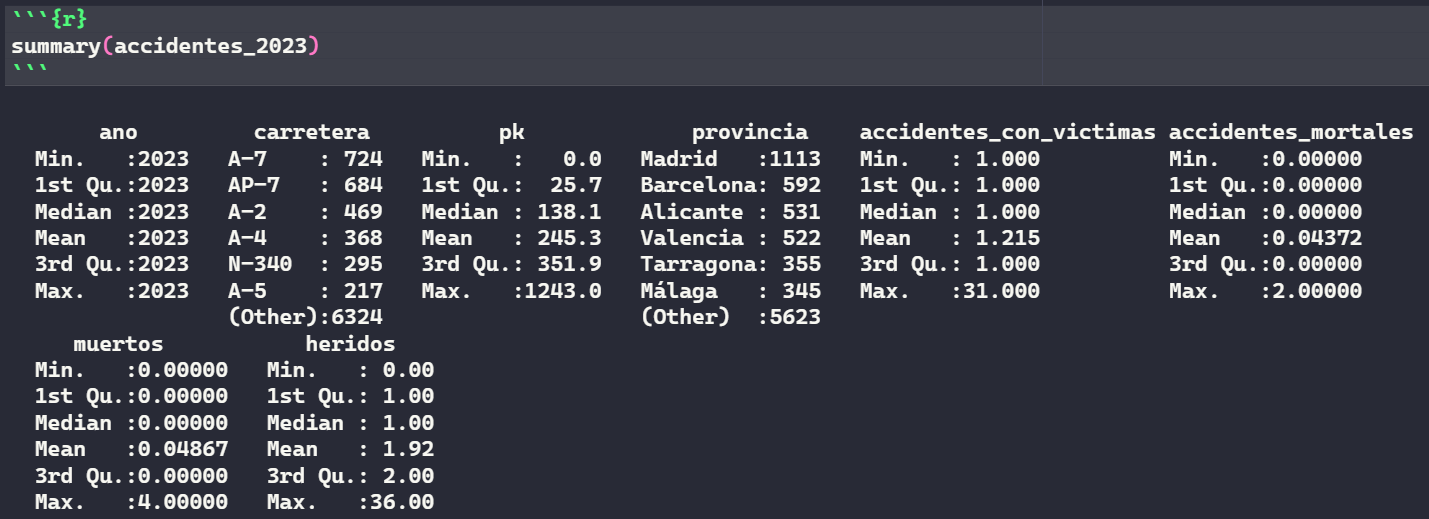
\includegraphics[width=\textwidth]{graficos4.3.1/sumaryac23.png} 
        \caption{Resultados del análisis descriptivo (2023).}
        \label{fig:acc_2023}
    \end{subfigure}
    \\ \vspace{0.4cm}
    \begin{subfigure}[b]{0.85\textwidth}
        \centering
        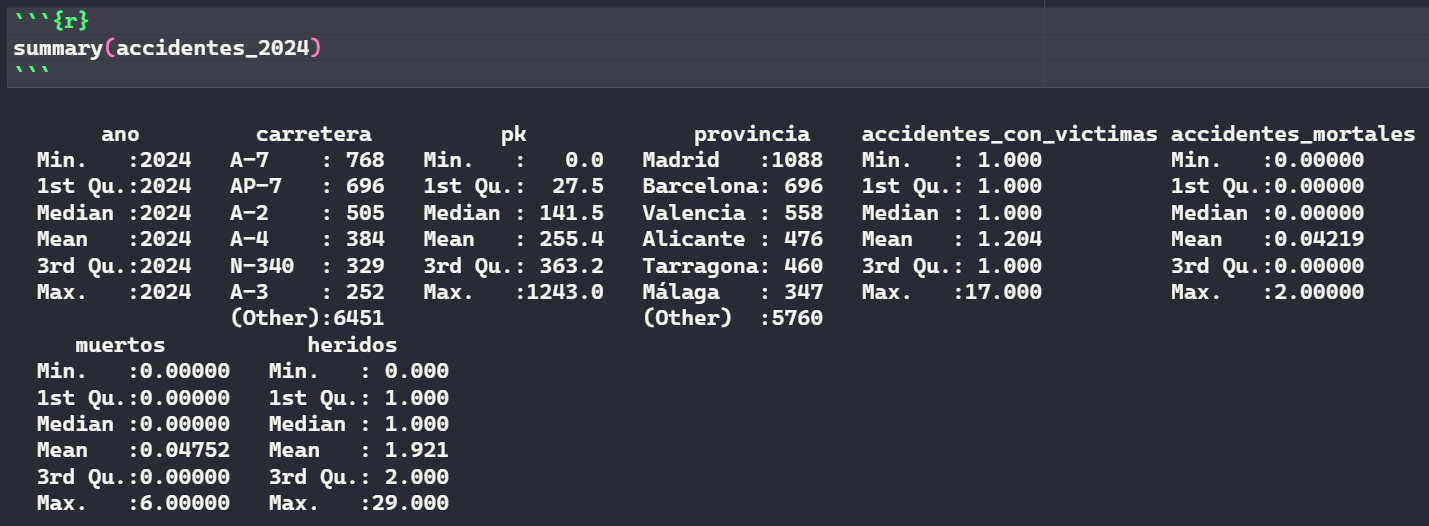
\includegraphics[width=\textwidth]{graficos4.3.1/sumaryac24.png} 
        \caption{Resultados del análisis descriptivo (2024).}
        \label{fig:acc_2024}
    \end{subfigure}
    \caption{Resultados de la función \textit{summary()} para la base de datos de Accidentes (2023-2024).}
    \label{fig:summary_accidentes}
\end{figure}

\subsubsection{Base de datos Tramos}

El análisis de los estadísticos descriptivos globales mediante la función \textit{summary()} sobre las bases de datos de intensidades de tráfico correspondientes a las campañas anuales de 2023 y 2024 arrojó una estructura de datos altamente consistente, caracterizada por los siguientes hallazgos analíticos:

\begin{itemize}
    \item \textbf{Variables Descriptivas y Geográficas (carretera, provincia, tipo\_via):} El volumen total de segmentos viales inventariados se estabilizó de forma homogénea en 7262 tramos para el año 2023 y 7248 para 2024. Geográficamente, la distribución espacial de la infraestructura permanece casi idéntica entre ambos periodos, siendo las provincias de Burgos (315 tramos en 2023 y 312 en 2024) y León (277 en ambos años) las que concentran la mayor cantidad de divisiones físicas de la red estatal. Administrativamente, la categoría de \textit{Carretera convencional} predomina de manera absoluta en el territorio nacional con más de 4400 segmentos anuales, seguida por el formato de \textit{Autovía}, que contabiliza 2134 tramos en 2023 y 2139 en 2024.
    
    \item \textbf{Variables de Localización Espacial (pk\_inicial, pk\_final):} La extensión lineal de la muestra abarca ejes de gran longitud que alcanzan un valor máximo de punto kilométrico final situado en los 1243.9 km. De forma crítica para el control de calidad, el indicador de valor mínimo reveló la existencia de registros numéricos negativos. En concreto, se aislaron dos tramos ubicados en las provincias de Toledo y Badajoz con puntos de inicio en los kilómetros $-0.37$ y $-0.75$, respectivamente, que finalizan en el kilómetro 0 (en 2024, el de la N-432 finaliza en el 0.005).
    
    Aunque en una primera inspección este hallazgo podría interpretarse como un fallo en la base de datos, se trata de valores reales y administrativos. En la ingeniería de tráfico, los puntos kilométricos negativos responden a ampliaciones físicas de la calzada que se ejecutan en sentido previo al origen histórico de la vía (su Kilómetro 0 original). Para evitar la re-numeración completa de toda la carretera, se asigna un kilometraje negativo a estos nuevos anexos. Al tratarse de una métrica espacial verídica, y dado que la diferencia matemática para calcular la longitud del tramo sigue arrojando una distancia positiva ($0 - (-0.37) = 0.37$ km), se determinó conservar estos registros intactos para no alterar la integridad de la muestra.
        
    Además, en la base de 2023 se detectó un tramo de la N-211A (Teruel) cuyo punto kilométrico final es menor que el inicial (214.000 frente a 207.875). Al tratarse de un único tramo entre más de 7000, se conservó en la base de datos; no obstante, al ser su longitud negativa, no puede asignársele ningún accidente y sus índices quedan con valor cero.
    
    \item \textbf{Indicadores de Carga Vehicular (imd\_total, imd\_ligeros, imd\_pesados):} Las variables continuas asociadas a la Intensidad Media Diaria evidencian la enorme dispersión y el comportamiento asimétrico del flujo circulatorio en España. El tráfico total presenta un espectro que oscila desde mínimos testimoniales de apenas 10 vehículos diarios en 2023 y 7 en 2024 en zonas rurales aisladas, hasta medianas nacionales que rondan los 6000 vehículos/día (6025 en 2023 y 6158 en 2024). Por su parte, los valores máximos absolutos alcanzan magnitudes críticas que alcanzan los 205501 vehículos diarios en 2023 y los 207675 en 2024, actuando estadísticamente como \textit{outliers} severos que identifican los accesos a las grandes coronas metropolitanas. Finalmente, la intensidad de vehículos pesados (\textit{imd\_pesados}) exhibe un valor medio sostenido de aproximadamente 1800 vehículos pesados al día en ambos años, registrando picos máximos de 41346 en 2023 y 36360 en 2024; un factor de vulnerabilidad estructural de gran interés para correlacionar posteriormente con los índices de siniestralidad severa.
\end{itemize}

\begin{figure}[H] 
    \centering
    
    \begin{subfigure}[b]{0.75\textwidth}
        \centering
        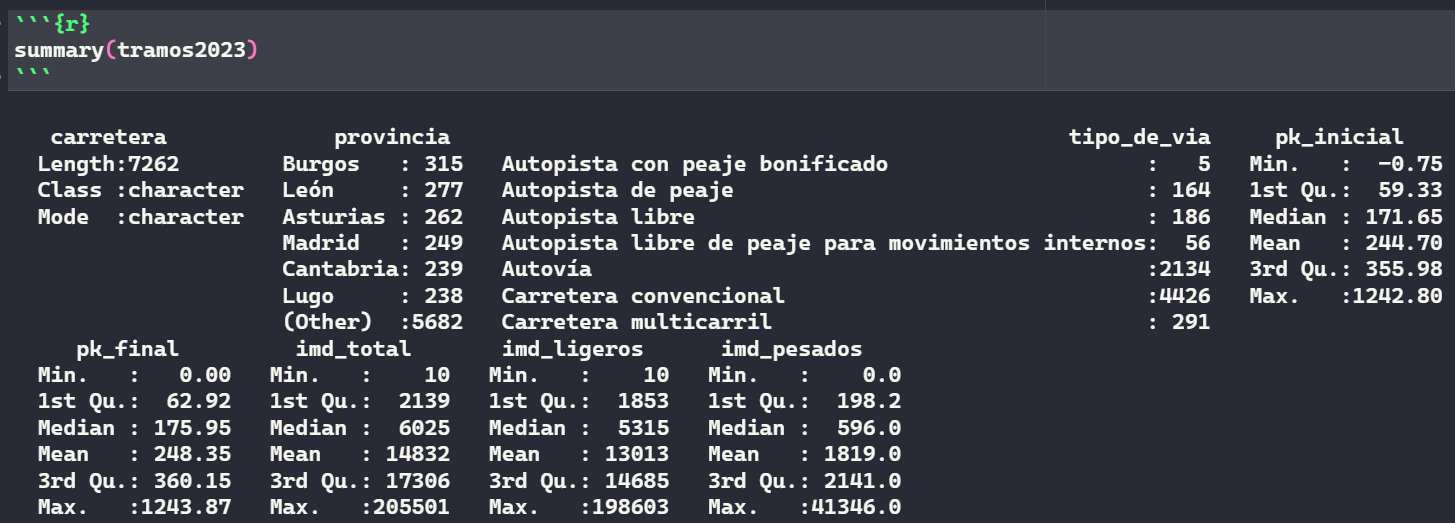
\includegraphics[width=\textwidth]{graficos4.3.1/sumarytr23.png} 
        \caption{Resultados del análisis descriptivo de Tramos (2023).}
        \label{fig:tramos_summary_2023}
    \end{subfigure}
    \\ \vspace{0.3cm}
    
    \begin{subfigure}[b]{0.75\textwidth}
        \centering
        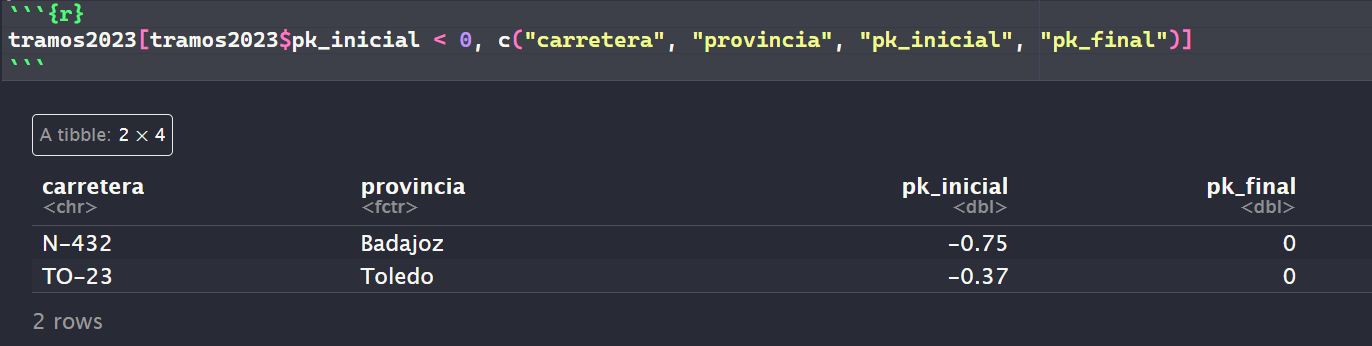
\includegraphics[width=\textwidth]{graficos4.3.1/trpkneg23.png} 
        \caption{Registros con puntos kilométricos iniciales negativos (2023).}
        \label{fig:tramos_negativos_2023}
    \end{subfigure}
    \\ \vspace{0.5cm} 
    
    \begin{subfigure}[b]{0.75\textwidth}
        \centering
        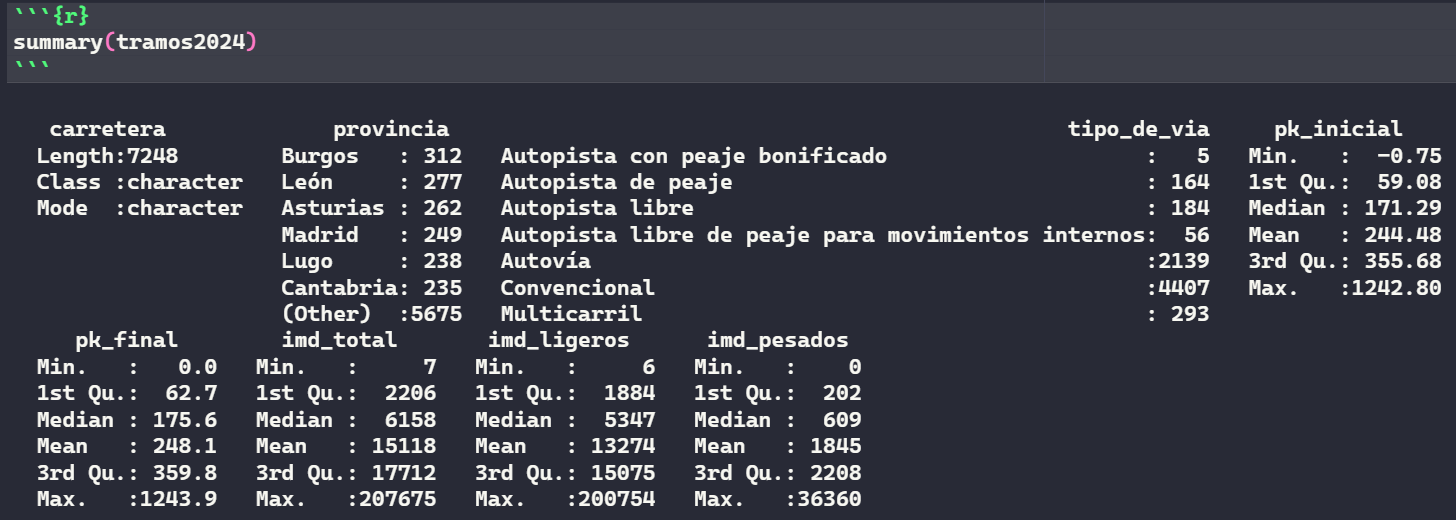
\includegraphics[width=\textwidth]{graficos4.3.1/sumarytr24.png} 
        \caption{Resultados del análisis descriptivo de Tramos (2024).}
        \label{fig:tramos_summary_2024}
    \end{subfigure}
    \\ \vspace{0.3cm}
    
    \begin{subfigure}[b]{0.75\textwidth}
        \centering
        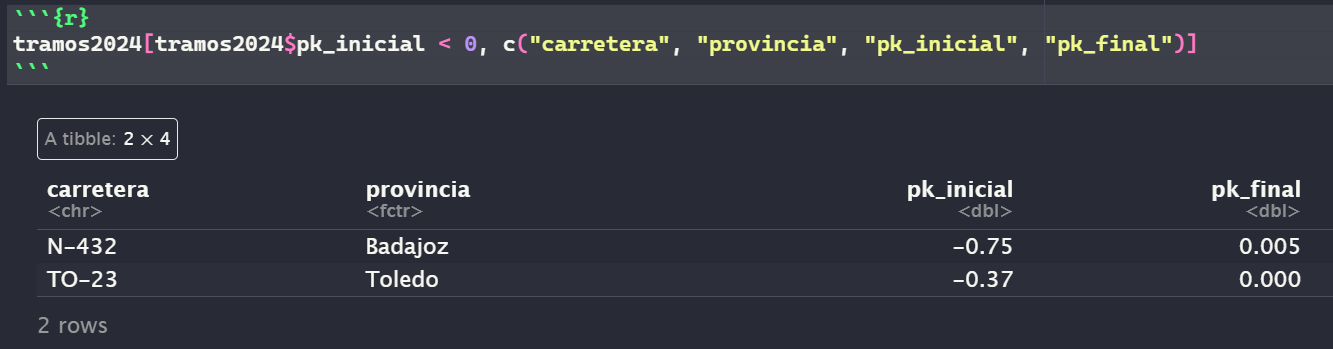
\includegraphics[width=\textwidth]{graficos4.3.1/trpkneg24.png} 
        \caption{Registros con puntos kilométricos iniciales negativos (2024).}
        \label{fig:tramos_negativos_2024}
    \end{subfigure}
    
    % Caption global
    \caption{Análisis exploratorio, estadísticos descriptivos y control de calidad para la base de datos de Tramos (2023--2024).}
    \label{fig:summary_tramos_completo}
\end{figure}

\subsection{Detección de Valores Atípicos (Outliers) mediante Análisis Visual}

Por otro lado, la identificación de valores extremos cuantitativos se abordó mediante técnicas de representación gráfica en R. Estas observaciones se definen como aquellos registros que presentan un comportamiento inusual y se desvían notablemente de la tendencia general de la muestra. La herramienta visual utilizada fue:

\begin{itemize}

    \item \textbf{Diagramas de Caja y Bigotes (\textit{Boxplots}):} Generamos diagramas de cajas para variables como la IMD. Esta herramienta nos permite visualizar de forma clara la mediana, los cuartiles y, sobre todo, identificar como \textit{outliers} aquellos puntos individuales que se salen de los límites (los ``bigotes'' del gráfico).
       
\end{itemize}

Tras la inspección visual, se observó la presencia de múltiples \textit{outliers}, que corresponden a los tramos de mayor tráfico, previsiblemente situados en las autovías y autopistas de las grandes áreas metropolitanas (como Madrid y Barcelona), cuyas mediciones de tráfico superan drásticamente la media del país. Dado que estos registros extremos constituyen mediciones reales y representan los sectores con mayor exposición al riesgo de siniestralidad, la decisión metodológica adoptada fue no eliminar ni transformar estos valores atípicos para las fases de modelado y minería de datos, ya que su eliminación sesgaría el análisis de los puntos críticos de la red.

\subsubsection{Base de Datos de Accidentes}

En el conjunto de registros de siniestralidad, la variable crítica para comprender la dispersión geográfica de los eventos es el punto kilométrico ($pk$). A continuación, las Figuras~\ref{fig:boxplot_pk_2023} y~\ref{fig:boxplot_pk_2024} exponen su comportamiento analítico para los dos periodos de estudio de manera aislada.

\clearpage

\begin{figure}[H]
    \centering
    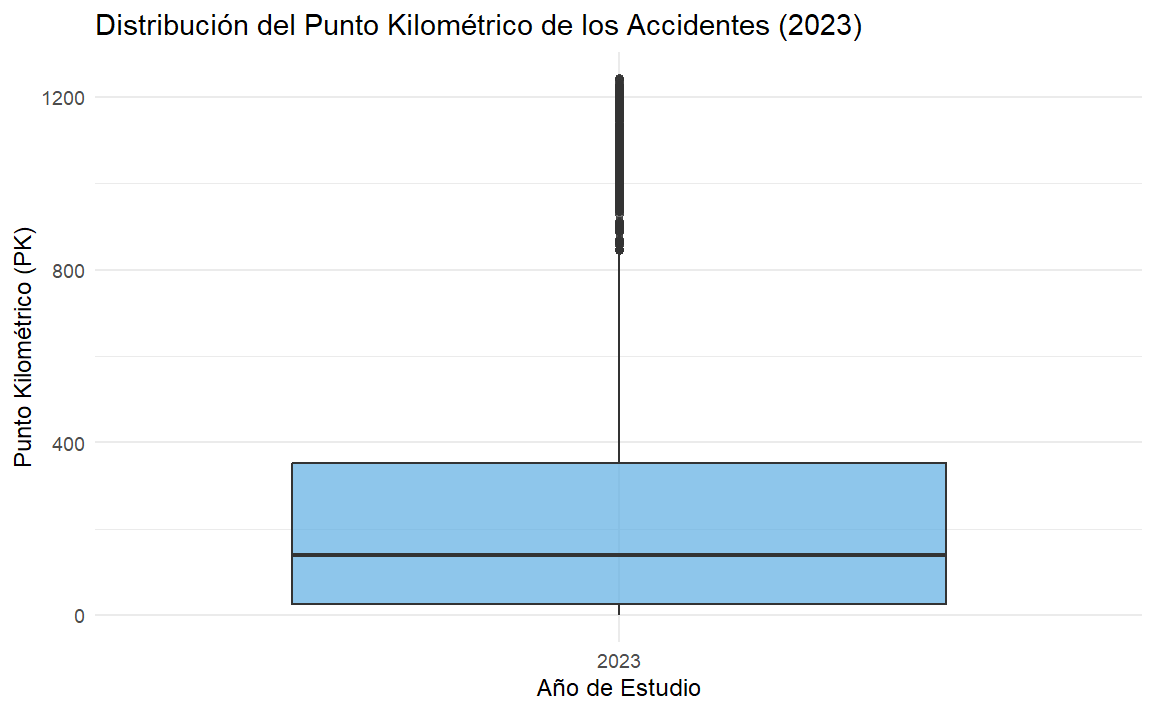
\includegraphics[width=0.85\textwidth]{graficos4.3.2/boxplot_pk_2023.png}
    \caption{Diagrama de caja para la localización de accidentes por Punto Kilométrico (PK) - Tabla 2023.}
    \label{fig:boxplot_pk_2023}
\end{figure}

\begin{figure}[H]
    \centering
    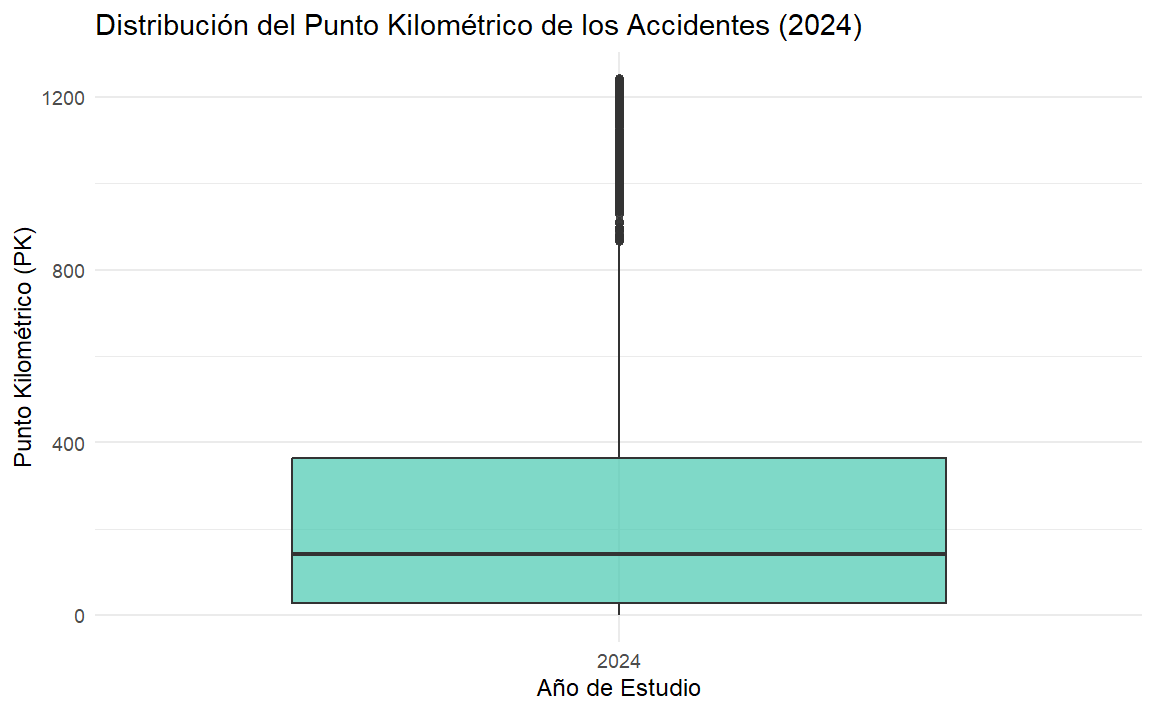
\includegraphics[width=0.85\textwidth]{graficos4.3.2/boxplot_pk_2024.png}
    \caption{Diagramas de caja para la localización de accidentes por Punto Kilométrico (PK) - Tabla 2024.}
    \label{fig:boxplot_pk_2024}
\end{figure}

Al examinar la distribución espacial, se identifica una morfología asimétrica positiva idéntica en ambos periodos de tiempo. El 75 \% de los registros se sitúa por debajo del km 351.9 en 2023 y del km 363.2 en 2024. 

\vspace{0.5cm}

Por otro lado, por encima del bigote superior aparece una línea densa de puntos individuales que se extiende hasta el km 1243.0. Estos puntos no son errores, sino accidentes ocurridos en los kilómetros finales de las carreteras de mayor longitud de la red (como la A-7 o la N-340). Por ello, se decidió conservarlos en el análisis, ya que de lo contrario se perderían ubicaciones con accidentes reales en las rutas más largas.

\subsubsection{Base de Datos de Tramos: Exposición al Tráfico}

El análisis visual de la infraestructura de tramos se concentra en aislar aquellos segmentos cuya Intensidad Media Diaria (\textit{imd\_total}) escapa drásticamente al comportamiento de las medias nacionales debido a la saturación vial.

\begin{figure}[H]
    \centering
    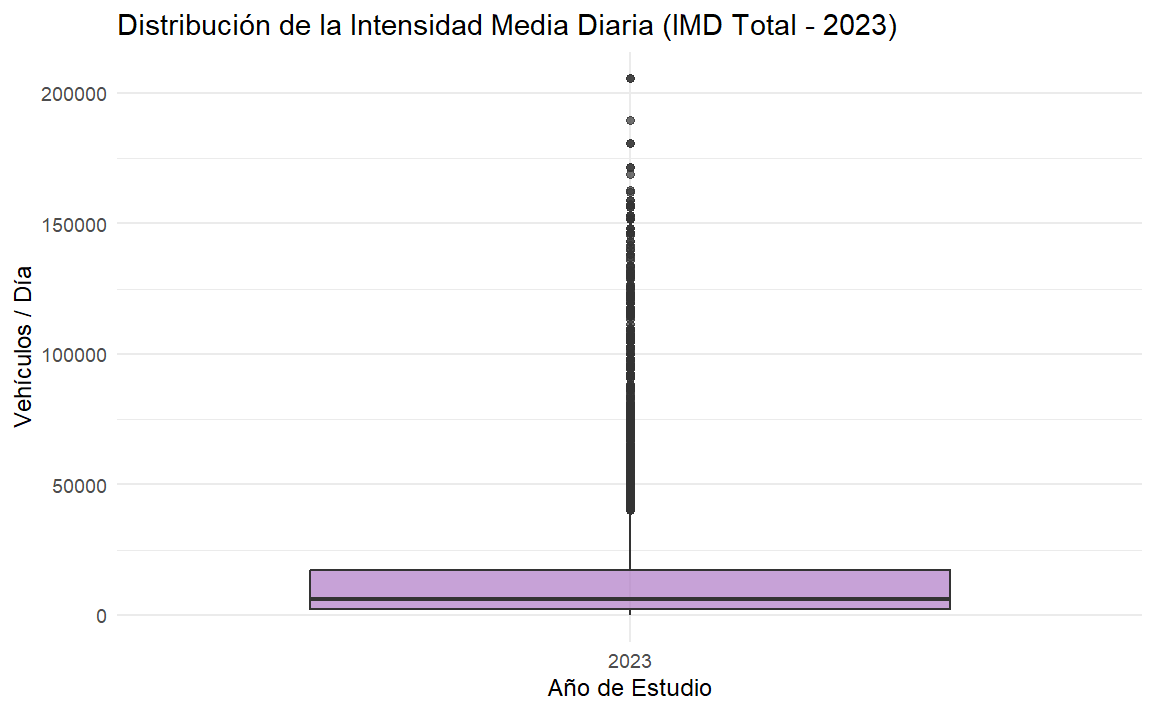
\includegraphics[width=0.85\textwidth]{graficos4.3.2/boxplot_imd_2023.png}
    \caption{Diagrama de caja para la Demanda de Tráfico - Tabla 2023.}
    \label{fig:boxplot_imd_2023}
\end{figure}

\clearpage

\begin{figure}[H]
    \centering
    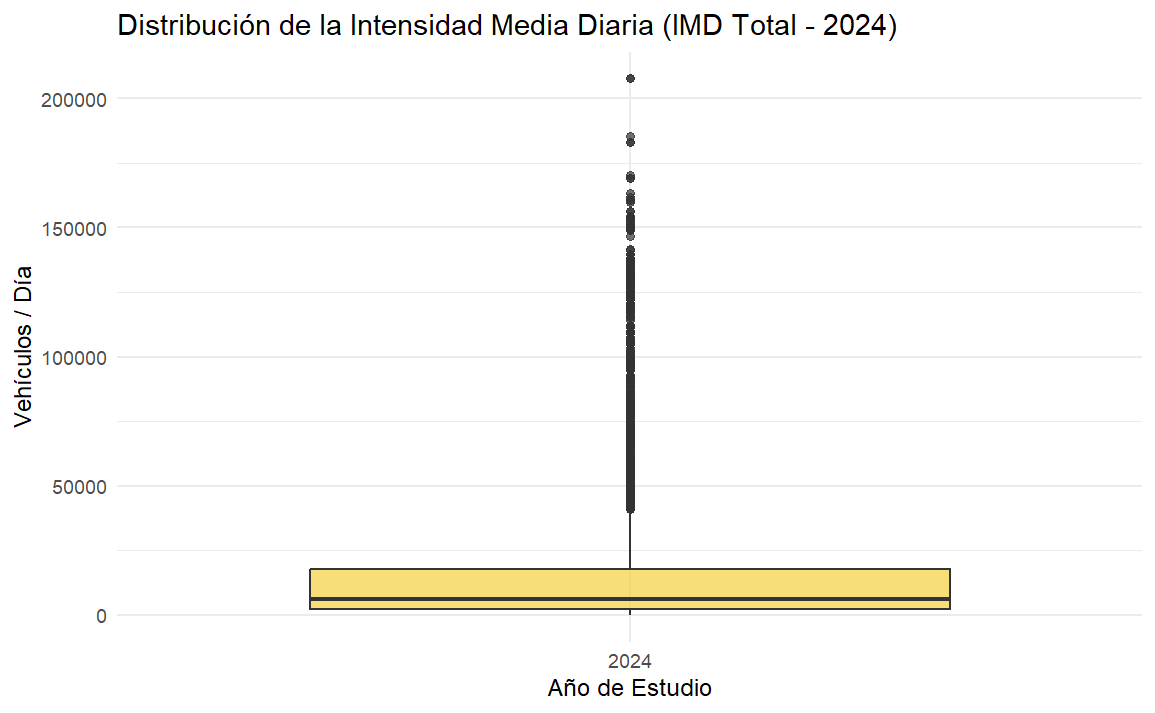
\includegraphics[width=0.85\textwidth]{graficos4.3.2/boxplot_imd_2024.png}
    \caption{Diagramas de caja para la Demanda de Tráfico - Tabla 2024.}
    \label{fig:boxplot_imd_2024}
\end{figure}

Los diagramas de caja de la variable \textit{imd\_total} (Figuras~\ref{fig:boxplot_imd_2023} y~\ref{fig:boxplot_imd_2024}) también reflejan esta asimetría positiva extrema, ya que los cuerpos de caja están ubicados en valores inferiores (con una mediana nacional de 6025 vehículos/día en 2023 y 6158 en 2024), pero en el límite superior hay una columna muy pronunciada de \textit{outliers} que alcanza los límites superiores del gráfico.

\vspace{0.5cm}

Los valores que corresponden al flujo de tráfico son enormes, al igual que picos como los alcanzados en 2023 con 205501 vehículos/día y en 2024 con 207675 vehículos/día. Lejos de ser casos atípicos o fallos técnicos, reflejan una representación realista del estado físico de las autopistas y circunvalaciones alrededor del centro metropolitano del país, que se encuentran en los alrededores de las aglomeraciones más importantes (principalmente Madrid y Barcelona), por lo que es necesario conservar esta información sin modificaciones para una representación correcta de la interacción entre vehículos y los riesgos de red viaria. 

\section{Selección de Variables}

Una vez completada la evaluación de calidad analítica y la tipificación factorial de los atributos cualitativos, nos adentramos en la etapa de selección de variables antes de la fusión de tablas. En la minería de datos, este paso resulta fundamental para reducir el espacio de características a los únicos atributos que puedan tener  poder predictivo, o que sean esenciales como índices para la indexación espacial  y para evitar el ruido de información  o atributos de varianza nula, que penalizarían   la eficiencia  del algoritmo computacional.

\vspace{0.5cm}

El proceso de selección se realizó de forma individual y paralela en los conjuntos de datos de Accidentes e Intensidades de Tráfico (Tramos), debido a que esta información es completamente parametrizada por su cuenta para las tablas 2023 y 2024 en esta fase del marco metodológico.

\subsection{Atributos Seleccionados de la Base de Datos de Accidentes}

En las matrices correspondientes a la siniestralidad de los años 2023 y 2024, se determinó conservar las siguientes variables debido a su relevancia relacional y analítica:

\begin{itemize}
    \item \textbf{\textit{carretera} y \textit{provincia}:} Se seleccionaron de forma obligatoria al actuar como los dos primeros criterios de indexación geográfica fundamentales para el posterior proceso de fusión con la infraestructura de tramos.
    
    \item \textbf{\textit{pk} (Punto Kilométrico):} Es la variable continua de posicionamiento lineal que identifica la coordenada exacta de la colisión. Resulta imprescindible para evaluar de forma condicional si el suceso pertenece al rango físico de un segmento de carretera.
    
    \item \textbf{\textit{accidentes\_con\_victimas}, \textit{accidentes\_mortales}, \textit{muertos} e \textit{heridos}:}  Se mantuvieron en su totalidad ya que corresponden a variables dependientes o de respuesta del estudio. 
\end{itemize}

\subsection{Atributos Seleccionados de la Base de Datos de Tramos (IMD)}

Por su parte, de las matrices descriptivas de la infraestructura viaria estatal, se seleccionaron los siguientes componentes estructurales y de demanda vehicular:

\begin{itemize}
    \item \textbf{\textit{carretera} y \textit{provincia}:} Conservadas bajo la misma premisa relacional para garantizar la correspondencia de las claves de unificación en el cruce de tablas.
    
    \item \textbf{\textit{tipo\_de\_via}:} Variable categórica factor esencial que clasifica el diseño de la carretera, permitiendo segregar posteriormente el comportamiento del riesgo entre vías de gran capacidad y calzadas convencionales.
    
    \item \textbf{\textit{pk\_inicial} y \textit{pk\_final}:} Delimitadores numéricos continuos que marcan el principio y el fin de la cobertura de cada tramo de aforo, estableciendo el intervalo geométrico de absorción de accidentes.
    
    \item \textbf{\textit{imd\_total}, \textit{imd\_ligeros} e \textit{imd\_pesados}:} Constituyen el núcleo de la dimensión preventiva y de exposición del modelo. Ponderan de forma matemática el volumen bruto de circulación y su desagregación por tipología de transporte, factores determinantes en la probabilidad de conflicto vial.
\end{itemize}

\subsection{Atributos Excluidos y Justificación Metodológica}

Bajo criterios de eficiencia y coherencia estadística, se procedió a la eliminación neta de la columna original de los archivos brutos al considerarse irrelevante para las fases de modelado supervisado:

\begin{itemize}
    \item \textbf{\textit{ano} (En el repositorio de Accidentes):} Debido a que la metodología de este trabajo procesa y analiza las bases de datos de cada campaña anual de forma estrictamente individualizada y segregada en el tiempo, mantener el atributo del año calendario dentro de su respectiva matriz introduce una columna con varianza igual a cero (una constante), aportando nula información marginal a los modelos predictivos.
\end{itemize}

\section{Fusión e Integración de Datos}

La etapa final del preprocesamiento consiste en la integración de las dos fuentes de información principales: el registro de siniestralidad (Accidentes) y el inventario de tramos de aforo (IMD). Dado que ambas fuentes presentan estructuras distintas (los accidentes se localizan en un punto kilométrico y los tramos en un intervalo), cada accidente se ha asignado al tramo cuyo intervalo de puntos kilométricos lo contiene.

\subsection{Metodología de Fusión}

La integración se ha realizado emparejando cada registro de accidentes con el tramo de aforo que le corresponde según su carretera, su provincia y su punto kilométrico, mediante los siguientes pasos:

\begin{enumerate}
    \item \textbf{Normalización de Identificadores:} Antes del cruce se unificaron los nombres de las provincias entre ambas fuentes. En la base de accidentes de 2023, las carreteras situadas en Cantabria (como la A-8, la A-67, la N-634 o la S-10) aparecían con la provincia ``San Sebastián'', mientras que en la base de 2024 y en el inventario de tramos figuran en Cantabria, por lo que se recodificaron como Cantabria. En la base de 2024, los nombres de las provincias venían en mayúsculas, por lo que se adaptaron a la forma empleada en la base de tramos (por ejemplo, ALICANTE pasó a Alicante/Alacant).

    El número de registros de estas carreteras en Cantabria en 2024 es similar al que presentaban en 2023 bajo la provincia ``San Sebastián'', lo que respalda esta corrección.
    
    \item \textbf{Cruce por carretera y provincia:} Se unió cada registro de accidentes con todos los tramos de su misma carretera y provincia.
    
    \item \textbf{Filtrado por punto kilométrico:} De esas combinaciones se conservó únicamente aquella en la que el PK del accidente se encuentra dentro del intervalo del tramo ($\text{PK}_{\text{inicial}} \leq \text{PK} \leq \text{PK}_{\text{final}}$). Cuando un PK coincide exactamente con el límite entre dos tramos consecutivos, se asignó al tramo de menor PK inicial, de modo que cada registro pertenece a un único tramo.
    
    \item \textbf{Consolidación:} Los datos se han consolidado por años naturales (2023 y 2024) para preservar la independencia temporal de las muestras, facilitando así la posterior comparación interanual.
\end{enumerate}

\subsection{Auditoría de Integridad y Exclusiones}

Tras la ejecución del proceso de fusión, se ha realizado una auditoría para evaluar la calidad y completitud de la muestra resultante. La fusión entre las bases de datos de accidentes y de tramos de aforo (IMD) se realiza emparejando cada accidente con un tramo cuando coinciden la carretera y la provincia, y el punto kilométrico (PK) del accidente se sitúa dentro del intervalo $[\text{pk}_{\text{inicial}}, \text{pk}_{\text{final}}]$ de ese tramo. Cuando un accidente no cumple estas condiciones, queda excluido del conjunto final, y se clasifica en uno de los dos siguientes niveles de exclusión, que representan causas metodológicamente distintas:

\begin{itemize}
    \item \textbf{Nivel A (Ausencia de vía):} El par carretera–provincia del accidente no existe en absoluto en el inventario de tramos. Es decir, no hay ningún tramo de aforo registrado para esa carretera en esa provincia, independientemente del punto kilométrico. Esta situación refleja un problema de cobertura de red: la vía en la que ocurrió el accidente no está contemplada por el inventario de estaciones de aforo.
    
    \item \textbf{Nivel B (PK fuera de rango):} La carretera sí existe en el inventario de tramos para esa provincia, pero el punto kilométrico del accidente no cae dentro de ninguno de los intervalos $[\text{pk}_{\text{inicial}}, \text{pk}_{\text{final}}]$ registrados para esa vía. Esta situación refleja un problema de cobertura de segmento: existen huecos puntuales dentro de una vía que, en general, sí está mapeada.
\end{itemize}

\vspace{0,5cm}

Cabe destacar que esta auditoría de exclusiones se aplica únicamente en la dirección accidentes → tramos, es decir, evaluando qué accidentes no logran encontrar un tramo de aforo compatible. La dirección inversa no requiere un análisis equivalente: un tramo de aforo sin accidentes asociados no constituye una pérdida de información, sino simplemente un tramo sin siniestralidad registrada en el periodo de estudio, que se refleja de forma natural como un valor de cero accidentes en la tabla de tramos fusionada.

\vspace{0,5cm}

Los resultados del proceso, desglosados por año, se resumen en la Tabla \ref{tab:auditoria_integracion}.

\vspace{0,5cm}

\textbf{Año 2023}

\begin{itemize}
    \item \textbf{Siniestros Integrados:} Un total de 10735 accidentes (97.31 \% del total) fueron asignados correctamente a sus tramos de aforo correspondientes, sobre un total original de 11032 accidentes con víctimas.
    
    \item \textbf{Siniestros No Integrados:} Se identificaron 297 accidentes (2.69 \%) que no pudieron ser vinculados, de los cuales 269 corresponden a ausencia de la vía en el inventario de tramos (Nivel A) y 28 a puntos kilométricos fuera de los rangos aforados (Nivel B).
\end{itemize}

\vspace{0,5cm}

\textbf{Año 2024}

\begin{itemize}
    \item \textbf{Siniestros Integrados:} Un total de 11080 accidentes (98.07 \% del total) fueron asignados correctamente a sus tramos de aforo, sobre un total original de 11298.
    \item \textbf{Siniestros No Integrados:} 218 accidentes (1.93 \%), de los cuales 190 se deben a ausencia de coincidencia de vía (Nivel A) y 28 a puntos kilométricos fuera de rango (Nivel B).
\end{itemize}

En términos de registros (puntos kilométricos), se integraron 8851 de 9081 en 2023 (97.47 \%) y 9207 de 9385 en 2024 (98.10 \%).

\begin{table}[htbp]
\centering
\caption{Resumen de la auditoría de integración accidentes--tramos por año}
\label{tab:auditoria_integracion}
\renewcommand{\arraystretch}{1.3}
\resizebox{\textwidth}{!}{%
\begin{tabular}{ccccc}
\toprule
\textbf{Año} & \textbf{Acc. con víctimas} & \textbf{Integrados} & \textbf{Nivel A (Sin Vía)} & \textbf{Nivel B (Fuera de PK)} \\
\midrule
2023 & 11032 & 10735 & 269  & 28 \\
2024 & 11298 & 11080  & 190 & 28 \\
\bottomrule
\end{tabular}%
}
\end{table}

El análisis de estos sucesos que no se han podido enlazar revela que no se trata de errores procedimentales, sino de una limitación intrínseca de la fuente: la mayoría de los casos de Nivel A se concentran en un número reducido de carreteras (véase Tabla \ref{tab:nivel_a_detalle}), mayoritariamente antiguos trazados o variantes identificados con el sufijo «a» (como la N-340a en Almería, Castellón o Málaga, la A-77a en Alicante o la N-2a en Girona) que no disponen de estaciones de aforo registradas en el inventario oficial, más que de errores puntuales de nomenclatura dispersos por todo el catálogo. A ellos se suman las carreteras de Ceuta (N-352 y N-354), cuyos tramos se eliminaron en el apartado 3.1.2 por no disponer de IMD. Entre 2023 y 2024 el número de accidentes de Nivel A se reduce de 269 a 190.

\begin{table}[htbp]
\centering
\caption{Carreteras con mayor número de accidentes sin coincidencia de vía (Nivel A, 2023)}
\label{tab:nivel_a_detalle}
\renewcommand{\arraystretch}{1.3}
\resizebox{\textwidth}{!}{%
\begin{tabular}{ccccccc}
\toprule
\textbf{Carretera} & \textbf{Provincia} & \textbf{N.º Reg.} & \textbf{Acc. Víctimas} & \textbf{Muertos} & \textbf{PK mín.} & \textbf{PK máx.} \\
\midrule
N-340a & Almería    & 39 & 41 & 1 & 384.0  & 558.5  \\
N-340a & Castellón  & 25 & 30 & 0 & 969.4  & 1057.2 \\
N-352  & Ceuta      & 10 & 27 & 0 & 0.3    & 2.5    \\
N-340a & Málaga     & 21 & 25 & 2 & 262.8  & 269.2  \\
A-77a  & Alicante   & 7  & 23 & 0 & 0.0    & 3.7    \\
N-2a   & Girona     & 19 & 23 & 1 & 0.2    & 725.0  \\
N-323a & Granada    & 13 & 17 & 0 & 117.1  & 463.7  \\
N-640a & Pontevedra & 8  & 12 & 0 & 235.7  & 238.4  \\
N-354  & Ceuta      & 7  & 10 & 0 & 0.5    & 4.1    \\
N-340a & Tarragona  & 3  & 7  & 0 & 1083.0 & 1172.0 \\
\bottomrule
\end{tabular}%
}
\end{table}

\vspace{0,5cm}

Desde una perspectiva metodológica, la exclusión de estos registros es una decisión necesaria y justificada. La ausencia de datos de carga vehicular (IMD) para estos tramos impediría el cálculo preciso del Índice de Peligrosidad, introduciendo sesgos derivados de la imputación artificial de valores. Por tanto, se ha priorizado la integridad estadística del conjunto final, conservando exclusivamente los datos que disponen de todas las variables necesarias para el análisis bidimensional posterior.

\section{Transformación de Variables}

Tras consolidar la matriz maestra mediante la integración espacial de los siniestros, se procedió a la etapa de transformación de variables. Este proceso tiene como finalidad generar nuevos indicadores sintéticos que permitan una interpretación más profunda de la seguridad vial y una comparación homogénea entre diferentes sectores de la red estatal.

\subsection{Generación del Identificador Secuencial de Tramo}

Con el objetivo de facilitar la trazabilidad espacial de los análisis, se detectó la necesidad de implementar una nomenclatura secuencial. Los registros originales carecían de un identificador jerárquico que permitiera seguir la progresión de una carretera de forma ordenada.

\vspace{0,5cm}

Para corregir esta carencia, se realizó un proceso de reordenamiento estructural:
\begin{enumerate}
    \item Se ordenó la totalidad de la red de carreteras alfanuméricamente por su \textit{carretera} y, de forma ascendente, por su \textit{pk\_inicial}.
    \item Se aplicó un contador dinámico agrupado por carretera, asignando a cada segmento la etiqueta \textit{``Tramo 1''}, \textit{``Tramo 2''}, etc.
\end{enumerate}
Este identificador permite visualizar la sucesión de segmentos a lo largo del eje vial y facilita la lectura de las tablas de resultados.

\subsection{Cálculo del Índice de Peligrosidad (IP)}

Se procedió a la normalización de la siniestralidad mediante el cálculo del \textbf{Índice de Peligrosidad (IP)}. Utilizar el recuento bruto de accidentes como única variable de respuesta induciría a un sesgo de exposición: las vías con mayor volumen circulatorio (IMD) o mayor longitud acumulan, por pura probabilidad, un número de incidentes superior.

\vspace{0,5cm}

Para obtener una métrica de riesgo relativo, se aplicó la fórmula estándar de ingeniería de tráfico sobre cada tramo $i$:

$$IP_i = \frac{N_i \cdot 10^8}{365 \cdot \text{IMD}_{\text{total},i} \cdot L_i}$$

Donde:
\begin{itemize}
    \item $N_i$: Número total de accidentes con víctimas registrados en el tramo.
    \item $\text{IMD}_{\text{total},i}$: Intensidad Media Diaria total (vehículos/día) del tramo.
    \item $L_i$: Longitud neta del tramo en kilómetros ($\text{pk}_{\text{final}} - \text{pk}_{\text{inicial}}$).
\end{itemize}

La constante $10^8$ permite escalar los valores resultantes a una magnitud fácilmente interpretable. Este indicador constituye el eje central del estudio, al permitir una comparación entre tramos con volúmenes de tráfico y extensiones dispares.

\vspace{0,5cm}

En la tabla de tramos, el índice se calcula una vez por tramo. En la tabla de accidentes, cada registro (punto kilométrico) recibe el índice del tramo al que pertenece, calculado con el total de accidentes de dicho tramo; por tanto, todos los puntos kilométricos de un mismo tramo comparten el mismo valor del índice.

\subsection{Cálculo del Índice de Mortalidad (IM)}

De forma complementaria al Índice de Peligrosidad, se ha incorporado el \textbf{Índice de Mortalidad (IM)} como indicador de severidad de la siniestralidad. Mientras que el IP permite identificar la frecuencia relativa de accidentes en función de la exposición al tráfico, el IM facilita la comprensión de las consecuencias físicas de dichos eventos, permitiendo distinguir entre tramos de alta siniestralidad y tramos de alta gravedad.

\vspace{0,5cm}

Para el cálculo de este indicador, se ha aplicado la misma lógica de normalización respecto al flujo vehicular, definiéndose la expresión matemática para cada tramo $i$ como:

$$IM_i = \frac{M_i \cdot 10^8}{365 \cdot \text{IMD}_{\text{total},i} \cdot L_i}$$

Donde:
\begin{itemize}
    \item $M_i$: Número total de personas fallecidas registradas en el tramo $i$.
    \item $\text{IMD}_{\text{total},i}$: Intensidad Media Diaria.
    \item $L_i$: Longitud del tramo.
\end{itemize}

La inclusión de esta métrica responde a la necesidad de evaluar la resiliencia de la infraestructura ante los impactos. Un tramo puede presentar un IP contenido, pero registrar un IM elevado, lo cual alertaría sobre deficiencias en la seguridad pasiva de la vía (tales como barreras de contención, señalización o falta de márgenes despejados) que convierten accidentes potencialmente leves en sucesos fatales. Este enfoque dual permite al futuro modelo de minería de datos realizar un diagnóstico mucho más preciso y orientado a la mitigación de riesgos críticos.

\section{Segmentación de Bases de Datos}
Tras el cálculo de los índices de riesgo, y como paso previo a la aplicación de los algoritmos de extracción de reglas, se determinó la necesidad metodológica de segmentar la información. Evaluar de forma conjunta la frecuencia de siniestros (Índice de Peligrosidad) y la severidad de los mismos (Índice de Mortalidad) en una misma matriz puede generar patrones redundantes o enmascarar relaciones específicas.

\vspace{0,5cm}

Por ello, se procedió a la partición de las dos matrices principales (Accidentes Detallados y Tramos Agregados) en ocho subconjuntos de datos independientes (Data Marts), aislados tanto por su año de estudio como por su variable de respuesta objetivo:

\begin{itemize}
    \item \textbf{Enfoque Situacional (Accidentes Detallados):} 
    \begin{itemize}
        \item Base de datos Accidentes IP 2023
        \item Base de datos Accidentes IM 2023
        \item Base de datos Accidentes IP 2024
        \item Base de datos Accidentes IM 2024
    \end{itemize}
    \item \textbf{Enfoque Macroestructural (Tramos Agregados):}
    \begin{itemize}
        \item Base de datos Tramos IP 2023
        \item Base de datos Tramos IM 2023
        \item Base de datos Tramos IP 2024
        \item Base de datos Tramos IM 2024
    \end{itemize}
\end{itemize}

Esta división garantiza que los posteriores algoritmos \textit{Apriori} y de \textit{Árboles de decisión} busquen patrones de alta accidentalidad de forma independiente a los patrones de alta mortalidad, ofreciendo conclusiones mucho más precisas para la ingeniería de tráfico.

\section{Análisis Exploratorio Bidimensional}

Para el estudio del conjunto de datos, es interesante realizar previamente un análisis bidimensional para determinar las relaciones e influencias que existen entre las variables de los conjuntos.

\vspace{0,5cm}

 El análisis exploratorio bidimensional se realizará de forma independiente para las cuatro bases de datos principales: Tramos 2023, Tramos 2024, Accidentes 2023 y Accidentes 2024. A diferencia de la fase de modelado posterior, en este estudio estadístico y visual se mantendrán juntos los dos índices (Peligrosidad y Mortalidad) dentro de cada respectiva tabla. Esta separación por año y origen de datos es metodológicamente necesaria, ya que cada conjunto posee una estructura y unas variables específicas que podrían distorsionar o enmascarar los resultados si se evaluaran de forma global.

\vspace{0,5cm}

Finalmente, se estudiará el resultado obtenido y se describirán las conclusiones al respecto.

\subsection{Base de datos de Tramos 2023}

Se realiza un análisis bidimensional entre cada una de las variables de la Base de Tramos de 2023, obteniendo los datos de correlación de cada par de variables entre sí, como se observa en la Figura~\ref{fig:corr_tr_2023}.

\begin{figure}[H]
     \centering
     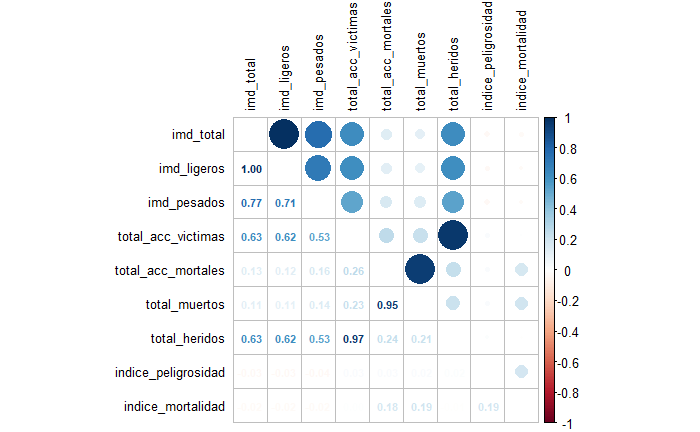
\includegraphics[width=\textwidth]{correlacion/corrtr23.png}
     \caption{Matriz de Correlación Tramos 2023}
     \label{fig:corr_tr_2023}
 \end{figure}

La matriz muestra fuertes correlaciones lógicas entre siniestros y víctimas, y asociaciones moderadas entre tráfico (IMD) y accidentes totales. Sin embargo, la correlación lineal de los Índices de Peligrosidad (IP) y Mortalidad (IM) con la intensidad del tráfico es casi nula. Esto indica que los índices no crecen con el volumen de vehículos como lo hace el recuento bruto de accidentes. No obstante, al dividir entre la IMD, los tramos con poco tráfico pueden alcanzar valores muy altos con pocos accidentes, aspecto que se analiza en el Capítulo~7.

\subsection{Base de datos de Tramos 2024}

Se realiza un análisis bidimensional entre cada una de las variables de la Base de Tramos de 2024, obteniendo los datos de correlación de cada par de variables entre sí, como se observa en la Figura~\ref{fig:corr_tr_2024}.

\begin{figure}[H]
     \centering
     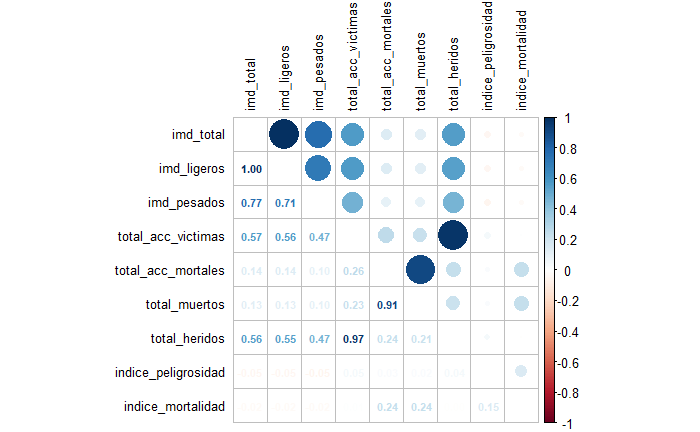
\includegraphics[width=\textwidth]{correlacion/corrtr24.png}
     \caption{Matriz de Correlación Tramos 2024}
     \label{fig:corr_tr_2024}
 \end{figure}

 El análisis de la matriz para el año 2024 revela un patrón estructural prácticamente idéntico al de 2023. Se mantienen las dependencias lógicas directas entre siniestros y víctimas, así como la asociación moderada con el volumen de tráfico. De igual modo, se mantiene la correlación casi nula de los Índices de Peligrosidad (IP) y Mortalidad (IM) respecto a la intensidad vehicular en los dos periodos estudiados.
 
\subsection{Base de datos de Accidentes 2023}

Se realiza un análisis bidimensional entre cada una de las variables de la Base de Accidentes de 2023, obteniendo los datos de correlación de cada par de variables entre sí, como se observa en la Figura~\ref{fig:corr_acc_2023}.

\begin{figure}[H]
     \centering
     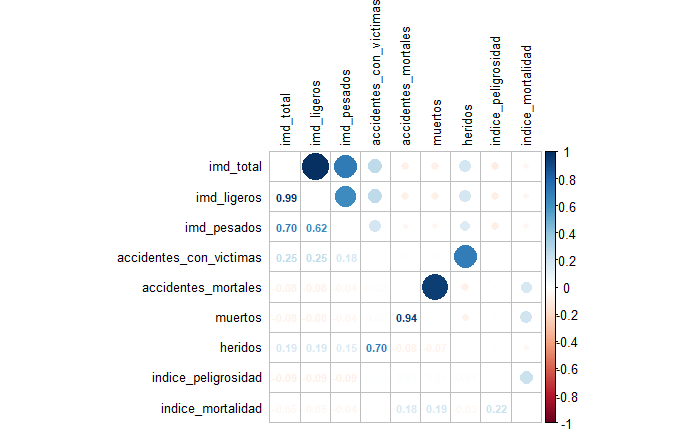
\includegraphics[width=\textwidth]{correlacion/corrac23.png}
     \caption{Matriz de Correlación Accidentes 2023}
     \label{fig:corr_acc_2023}
 \end{figure}

La matriz destaca una dependencia directa casi perfecta entre los siniestros mortales y el número de fallecidos (0.94), así como una fuerte asociación entre los accidentes con víctimas y los heridos (0.70). A diferencia de los datos agrupados por tramo, la relación del volumen de tráfico (IMD) con los accidentes en un punto kilométrico exacto es débil (0.25). Además, se confirma que los índices de peligrosidad y mortalidad tienen una correlación nula o ligeramente negativa respecto a la intensidad vehicular.

 \subsection{Base de datos de Accidentes 2024}

Se realiza un análisis bidimensional entre cada una de las variables de la Base de Accidentes de 2024, obteniendo los datos de correlación de cada par de variables entre sí, como se observa en la Figura~\ref{fig:corr_acc_2024}.

\begin{figure}[H]
     \centering
     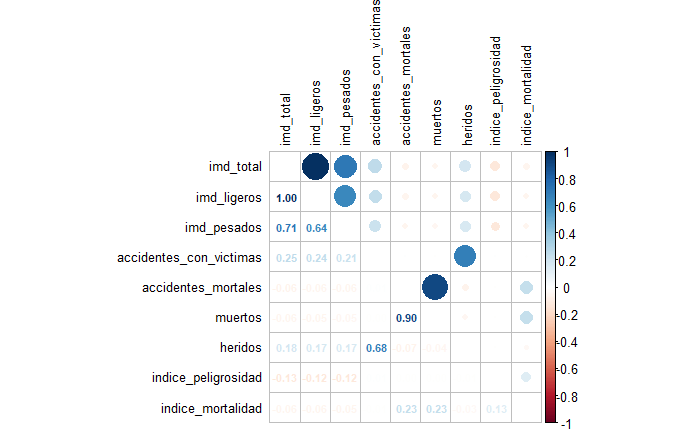
\includegraphics[width=\textwidth]{correlacion/corrac24.png}
     \caption{Matriz de Correlación Accidentes 2024}
     \label{fig:corr_acc_2024}
 \end{figure}

El comportamiento estadístico es prácticamente idéntico al de 2023. Las correlaciones lógicas entre la tipología del siniestro y su gravedad se mantienen muy altas (0.90 para los fallecidos y 0.68 para los heridos). Este resultado consolida la escasa relación lineal entre el tráfico absoluto y los incidentes de cada punto kilométrico.

\section{Estructura Definitiva del Conjunto de Datos}

Como resultado de todas las fases descritas en este capítulo (limpieza, fusión, transformación y segmentación), se obtuvieron las distintas tablas sobre las que operarán los algoritmos. 

\vspace{0.5cm}

A continuación se muestra un extracto de dos de ellas.

\subsection{Tabla Accidentes Detallados IP 2023}

\begin{table}[H]
    \centering
    \caption{Extracto de la tabla de accidentes - Índice de Peligrosidad (accidentes\_detallados\_ip\_2023)}
    \label{tab:accidentes_ip_2023}
    
    % PRIMERA PARTE DE LA TABLA (Primeras 8 columnas)
    \resizebox{\textwidth}{!}{%
    \begin{tabular}{llcccccc}
        \toprule
        \textbf{carretera} & \textbf{provincia} & \textbf{pk} & \textbf{acc\_con\_victimas} & \textbf{acc\_mortales} & \textbf{muertos} & \textbf{heridos} & \textbf{tipo\_de\_via} \\
        \midrule
        A-1 & Madrid & 12.9 & 1 & 0 & 0 & 1 & Autovía \\
        A-1 & Madrid & 13.0 & 3 & 0 & 0 & 4 & Autovía \\
        A-1 & Madrid & 13.1 & 2 & 0 & 0 & 3 & Autovía \\
        A-1 & Madrid & 13.2 & 2 & 0 & 0 & 4 & Autovía \\
        A-1 & Madrid & 13.6 & 2 & 0 & 0 & 2 & Autovía \\
        A-1 & Madrid & 13.7 & 2 & 0 & 0 & 6 & Autovía \\
        \bottomrule
    \end{tabular}
    }
    
    \vspace{0.4cm}
    \textit{\small (Continuación de columnas para las mismas observaciones)}
    \vspace{0.2cm}
    
    % SEGUNDA PARTE DE LA TABLA (Las 6 columnas restantes)
    \resizebox{\textwidth}{!}{%
    \begin{tabular}{cccccc}
        \toprule
        \textbf{imd\_total} & \textbf{imd\_ligeros} & \textbf{imd\_pesados} & \textbf{pk\_inicial} & \textbf{pk\_final} & \textbf{indice\_peligrosidad} \\
        \midrule
        205501 & 198603 & 6898 & 12.000 & 14.000 & 9.9989514 \\
        205501 & 198603 & 6898 & 12.000 & 14.000 & 9.9989514 \\
        205501 & 198603 & 6898 & 12.000 & 14.000 & 9.9989514 \\
        205501 & 198603 & 6898 & 12.000 & 14.000 & 9.9989514 \\
        205501 & 198603 & 6898 & 12.000 & 14.000 & 9.9989514 \\
        205501 & 198603 & 6898 & 12.000 & 14.000 & 9.9989514 \\
        \bottomrule
    \end{tabular}
    }
\end{table}


\subsection{Tabla Tramos IP 2023}

\begin{table}[H]
    \centering
    \caption{Extracto de la tabla de tramos - Índice de Peligrosidad (tramos\_detallados\_ip\_2023)}
    \label{tab:tramos_ip_2023}
    
    % PRIMERA PARTE DE LA TABLA (Primeras 7 columnas)
    \resizebox{\textwidth}{!}{%
    \begin{tabular}{llllccc}
        \toprule
        \textbf{carretera} & \textbf{nombre\_tramo} & \textbf{provincia} & \textbf{tipo\_de\_via} & \textbf{pk\_inicial} & \textbf{pk\_final} & \textbf{imd\_total} \\
        \midrule
        A-1 & Tramo 1 & Madrid & Autovía & 12.000 & 14.000 & 205501 \\
        A-1 & Tramo 2 & Madrid & Autovía & 14.000 & 16.800 & 205501 \\
        A-1 & Tramo 3 & Madrid & Autovía & 16.800 & 19.200 & 156111 \\
        A-1 & Tramo 4 & Madrid & Autovía & 19.200 & 20.400 & 156111 \\
        A-1 & Tramo 5 & Madrid & Autovía & 20.400 & 22.700 & 95706 \\
        A-1 & Tramo 6 & Madrid & Autovía & 22.700 & 33.700 & 64718 \\
        \bottomrule
    \end{tabular}
    }
    
    \vspace{0.4cm}
    \textit{\small (Continuación de columnas para las mismas observaciones)}
    \vspace{0.2cm}
    
    % SEGUNDA PARTE DE LA TABLA (Las 7 columnas restantes)
    \resizebox{\textwidth}{!}{%
    \begin{tabular}{ccccccc}
        \toprule
        \textbf{imd\_ligeros} & \textbf{imd\_pesados} & \textbf{total\_acc\_victimas} & \textbf{total\_acc\_mortales} & \textbf{total\_muertos} & \textbf{total\_heridos} & \textbf{indice\_peligrosidad} \\
        \midrule
        198603 & 6898 & 15 & 0 & 0 & 24 & 9.9989514 \\
        198603 & 6898 & 15 & 0 & 0 & 16 & 7.1421082 \\
        150636 & 5475 & 21 & 0 & 0 & 27 & 15.3561266 \\
        150636 & 5475 & 3 & 0 & 0 & 3 & 4.3874647 \\
        85626 & 10080 & 2 & 0 & 0 & 4 & 2.4892593 \\
        59242 & 5476 & 20 & 0 & 0 & 34 & 7.6969623 \\
        \bottomrule
    \end{tabular}
    }
\end{table}

\vspace{0.5cm}

La estructura para los datos del año 2024 y para los conjuntos enfocados en el Índice de Mortalidad (IM) mantiene esta misma arquitectura exacta, sustituyendo únicamente la variable dependiente final.

\vspace{0.5cm}

Con esta arquitectura de datos plenamente consolidada y depurada, se concluye la fase de preparación, dando paso a la aplicación teórica y práctica de la Minería de Datos.

%%%%%%%%%%%%% FIN DE CAPÍTULO 3. Preprocesamiento y Limpieza de Datos %%%%%%%%%%%%%%%%%%%

%%%%%%%%%%%%%%%%%%%%%%%%%%%%%%%% INICIO CAP 4 %%%%%%%%%%%%%%%%%%%%%%%%%%%%%%%%%%%%%%%%%%%
\setcounter{chapter}{4}
\chapter*{Capítulo 4 \\ \vspace{1cm} Conocimientos Previos}

\setcounter{section}{0}
\setcounter{subsection}{0}

\setcounter{chapter}{4}
\setcounter{figure}{0}\setcounter{table}{0}

\addcontentsline{toc}{chapter}{\protect\numberline{\thechapter}Conocimientos Previos}

Para comprender este trabajo es necesario definir previamente las técnicas empleadas y la utilidad de cada una de ellas. De esta forma, será más comprensible por qué las estamos usando y su finalidad. En concreto, en este capítulo se presentan las dos técnicas de minería de datos aplicadas: las reglas de asociación, con sus métricas de evaluación, la discretización de las variables y el funcionamiento del algoritmo \textit{Apriori}, y los árboles de clasificación, con su proceso de construcción, la poda para evitar el sobreajuste y las medidas empleadas para evaluar su rendimiento.


\section{Reglas de Asociación}

Las reglas de asociación son una técnica de aprendizaje no supervisado y de carácter descriptivo, que tiene como objetivo principal encontrar relaciones ocultas o patrones frecuentes dentro de un gran conjunto de datos. En concreto, buscan identificar qué elementos o características tienden a ocurrir de forma conjunta en una misma transacción. Estas técnicas asumen que todos los datos de entrada son categóricos, es decir, variables que describen cualidades o estados \cite{apuntes_teoria2025}. 

\vspace{0.5cm}

El origen de estas técnicas proviene del ámbito de la computación y el análisis comercial. Una anécdota famosa, probablemente apócrifa, ilustra su potencial: según se cuenta, un supermercado descubrió que los hombres de entre 30 y 40 años que compraban pañales los viernes entre las 17:00 y las 19:00 horas eran muy propensos a llevar también cerveza en su carrito, y al mover el pasillo de las cervezas cerca del de los pañales se habría registrado un aumento en las ventas de ambos productos.

\vspace{0.5cm}

Para lograr este tipo de hallazgos, la eficacia de las reglas de asociación se apoya en un enfoque estadístico fundamentado en conceptos de correlación y probabilidad condicionada. Sin embargo, no están diseñadas para muestras de datos reducidas, ya que su cálculo requiere estructuras de datos especializadas y algoritmos capaces de procesar volúmenes masivos de información de forma eficiente.

\subsection{Conceptos básicos y Métricas de evaluación}

Para comprender matemáticamente el funcionamiento de estos algoritmos, es indispensable definir la terminología básica sobre la que operan \cite{apuntes_teoria2025}:

\begin{itemize}
    \item \textbf{Ítem:} Es el elemento individual básico o el valor de un atributo. Por ejemplo, en nuestro contexto, un ítem podría ser \textit{Tipo\_via = Autovía}.
    
    \item \textbf{Itemset (Conjunto de ítems):} Es una colección de uno o más ítems. Por ejemplo: \{\textit{Tipo\_via = Autovía}, \textit{IMD\_Pesados = Alto}\}.
    
    \item \textbf{Transacción:} Representa un conjunto de eventos o ítems que ocurren de forma conjunta y que están asociados de alguna forma. En una base de datos, equivaldría a una fila completa.
\end{itemize}

Matemáticamente, una regla de asociación se representa mediante una implicación del tipo ``Si A, entonces C'' ($A \Rightarrow C$). Aquí, el conjunto de ítems $A$ se denomina antecedente, mientras que al conjunto $C$ se le llama consecuente. Ambos no deben compartir elementos ($A$ y $C$ son disjuntos, $A \cap C = \emptyset$). Esta expresión no indica una implicación lógica estricta, sino una tendencia: cuando en una transacción ocurren los ítems de $A$, con cierta probabilidad también aparecen los de $C$.

\vspace{0.5cm}

No obstante, en grandes bases de datos se pueden generar miles de reglas. Para determinar la validez y el interés estadístico de una regla generada, se emplean principalmente tres métricas clásicas \cite{apuntes_teoria2025, practica_asociacion}. En las fórmulas, $A \cup C$ denota el conjunto de transacciones que contienen a la vez todos los ítems de $A$ y de $C$:


\begin{itemize}
    \item \textbf{Soporte (\textit{Support}):} Mide la frecuencia con la que ocurre la asociación en el conjunto de datos. Es la proporción de transacciones que contienen la unión de $A$ y $C$ respecto al total de transacciones en la base de datos ($N$). Ayuda a filtrar reglas que ocurren tan poco que carecen de relevancia estadística.
    
    $$ \text{Soporte}(A \Rightarrow C) = P(A \cup C) = \frac{\text{Frecuencia}(A \cup C)}{N} $$
    
    \item \textbf{Confianza (\textit{Confidence}):} Mide la fiabilidad de la regla. Es la probabilidad condicionada de que una transacción contenga $C$ dado que ya contiene $A$.
    
    $$ \text{Confianza}(A \Rightarrow C) = P(C \mid A) = \frac{\text{Soporte}(A \cup C)}{\text{Soporte}(A)} $$
    
    \item \textbf{Elevación (\textit{Lift}):} Mide la razón de la confianza de la regla frente a la proporción de transacciones que contienen el consecuente. Un valor de Lift $> 1$ indica una asociación positiva (la ocurrencia de A aumenta la probabilidad de C o que la co-ocurrencia es mayor a la esperada por azar), mientras que un valor $< 1$ indica dependencia negativa. También se tiene el caso de Lift $=$ 1, que es el caso de independencia.
    
    $$ \text{Lift}(A \Rightarrow C) = \frac{\text{Confianza}(A \Rightarrow C)}{\text{Soporte}(C)} = \frac{P(A \cup C)}{P(A) \cdot P(C)} $$
    
\end{itemize}

\subsection{El problema del preprocesado: Discretización}

Una de las principales limitaciones matemáticas de la técnica de reglas de asociación es que asume que todos los datos de entrada son categóricos o nominales. 

\vspace{0.5cm}

Si se dispone de variables continuas, como es el caso de la Intensidad Media Diaria (IMD) o el Índice de Peligrosidad (IP) en este estudio, es imperativo someterlas a un proceso de \textbf{discretización}. Esto implica particionar el dominio numérico de la variable en intervalos o categorías (\textit{bins}). Por ejemplo, convertir el valor numérico continuo de la IMD en etiquetas categóricas como ``Baja'', ``Media'' o ``Alta''.

\vspace{0.5cm}

Este proceso es crítico porque una mala discretización puede conllevar pérdida de información. Si los intervalos son demasiado pequeños, no se generarán ítems frecuentes y el algoritmo no encontrará reglas; si son demasiado amplios, se perderán los matices y el comportamiento de los valores extremos (\textit{outliers}). Además, los datos deben organizarse en formato transaccional (una matriz binaria ítem-transacción) para que el algoritmo determine qué ítems aparecen (1) o no (0) \cite{apuntes_teoria2025}.

\paragraph{Métodos de discretización.} 

\vspace{0.5cm}

Existen varias estrategias para particionar una variable continua:
\begin{itemize}
    \item \textbf{Igual anchura} (\textit{equal width}): divide el rango de la variable en $k$ intervalos de igual longitud. Es simple, pero muy sensible a los valores extremos: con variables muy asimétricas, casi todas las observaciones caen en los primeros intervalos y el resto quedan prácticamente vacíos.
    
    \item \textbf{Igual frecuencia} (\textit{equal frequency}): los puntos de corte son cuantiles, de modo que cada intervalo contiene aproximadamente el mismo número de observaciones. Es robusta ante la asimetría y proporciona ítems con un soporte similar, pero produce intervalos de anchura muy dispar y no funciona bien cuando hay muchos valores repetidos.
    
    \item \textbf{Basada en agrupamiento} (\textit{clustering}): se aplica un algoritmo como $k$-medias sobre la variable y cada grupo es una categoría. Se adapta a la forma de la distribución, pero depende del número de grupos $k$ y de la inicialización.
    
    \item \textbf{Supervisada}: elige los puntos de corte usando una variable objetivo, por ejemplo mediante criterios basados en entropía. Genera categorías informativas para ese objetivo, pero lo introduce como sesgo y exige definirlo de antemano.
    
    \item \textbf{Por umbrales de expertos o normativos}: cortes con significado propio en el dominio de aplicación.
\end{itemize}
En el Capítulo~5 se emplea la discretización por igual frecuencia (sextiles), cuya elección se justifica allí en función de las características de las variables del estudio.
 

\subsection{Descripción del Algoritmo y Generación de Reglas}

Los algoritmos de reglas de asociación, como el clásico \textit{Apriori}, dividen su ejecución en dos fases fundamentales:

\vspace{0.5cm}

\textbf{1. Generación de itemsets frecuentes:} \\

En esta fase, el algoritmo identifica todas las combinaciones de ítems cuyo soporte es igual o superior a un umbral mínimo establecido por el analista (\textit{minsup}). Como explorar todas las combinaciones posibles tiene una complejidad combinatoria enorme, el algoritmo se basa en el \textit{Principio Apriori} (antimonotonía del soporte), que establece dos propiedades para optimizar la búsqueda:

\begin{itemize}
    \item Todo subconjunto de un conjunto de ítems frecuente, también debe ser frecuente.
    
    \item Si un conjunto de ítems no es frecuente, ninguno de sus superconjuntos lo será, lo que permite podar grandes ramas del espacio de búsqueda.
\end{itemize}

 \begin{figure}[H]
     \centering
     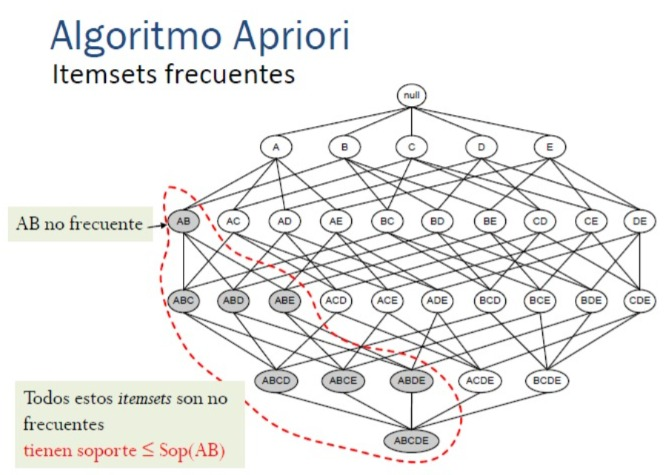
\includegraphics[width=0.7\textwidth]{capitulo4/podaapriori.jpeg}
     \caption{Representación del espacio de búsqueda y poda en el algoritmo Apriori.}
     \label{fig:poda_apriori}
 \end{figure}


Gracias a estas propiedades, el algoritmo evita el ineficiente enfoque de ``fuerza bruta'', que consistiría en generar y evaluar todas las combinaciones al mismo tiempo, y opta por una solución estructurada en etapas. El algoritmo Apriori aplica esta búsqueda de forma iterativa:

\begin{itemize}
    \item En primer lugar, construye conjuntos formados por un solo ítem ($n=1$) y filtra aquellos que superan el soporte mínimo.
    
    \item Posteriormente, utiliza esos resultados para construir y evaluar conjuntos de dos ítems ($n=2$).

    \item El procedimiento se repite sucesivamente, aumentando el tamaño $n$ hasta que ya no existan conjuntos de ítems que logren superar el soporte mínimo exigido.
\end{itemize}

Cabe destacar que, aunque el algoritmo Apriori centra su estrategia en reducir el número de candidatos, existen otras alternativas algorítmicas en la minería de datos, como DHP o FP-Growth, diseñadas para optimizar el proceso mediante la reducción del número de transacciones o el empleo de estructuras de datos más eficientes para las comparaciones \cite{practica_asociacion}.

\vspace{0.5cm}

\textbf{2. Generación de reglas a partir de itemsets frecuentes:} 

\vspace{0.5cm}

Una vez aislados los conjuntos frecuentes, el algoritmo genera todas las reglas de asociación posibles combinando sus elementos. Por ejemplo, si el conjunto $\{a, b, c\}$ es frecuente, se evaluarán reglas como $\{a, b\} \Rightarrow \{c\}$, $\{a\} \Rightarrow \{b, c\}$, etc. De todas ellas, solo se conservarán aquellas cuya \textbf{Confianza} supere el umbral mínimo fijado (\textit{minconf}).

\vspace{0.5cm}

Es importante destacar una propiedad matemática clave en esta fase generativa: a diferencia del soporte, la confianza general no es una medida anti-monótona. Sin embargo, las reglas generadas a partir de un mismo conjunto de ítems sí mantienen una relación anti-monótona respecto al número de elementos en el consecuente (la parte derecha de la regla). Esto significa que, siguiendo el ejemplo anterior, se cumplirá siempre que la confianza de $\{a, b\} \Rightarrow \{c\}$ será mayor o igual que la confianza de $\{a\} \Rightarrow \{b, c\}$ \cite{practica_asociacion}.  

\vspace{0.5cm}

\textbf{Limitaciones de la Confianza y Métricas Adicionales} 

\vspace{0.5cm}

No obstante, basar la validez de una regla de asociación únicamente en la confianza puede resultar engañoso en la práctica. Una regla con una confianza muy alta puede obtenerse simplemente porque el elemento consecuente es muy frecuente de por sí en el conjunto de datos global, y no porque exista una relación o dependencia real con el antecedente.  Para corregir este sesgo y filtrar aquellas reglas que sean triviales o que no aporten un conocimiento de valor, el algoritmo se apoya en métricas adicionales de evaluación:  

\begin{itemize}
\item \textbf{Leverage (Apalancamiento):} Mide la diferencia absoluta entre el soporte observado de ambos elementos juntos y el soporte que se esperaría si fueran estadísticamente independientes. Los valores mayores a 0 indican una relación positiva.
$$ \text{Leverage}(A \Rightarrow C) = P(A \cup C) - P(A)\,P(C) $$

\item \textbf{Conviction (Convicción):} Mide el grado de dependencia del consecuente respecto al antecedente. Valores superiores a 1 indican una mayor certeza de que el antecedente implica al consecuente, pudiendo llegar a infinito cuando la implicación es perfecta.

$$ \text{Conviction}(A \Rightarrow C) = \frac{1 - \text{Soporte}(C)}{1 - \text{Confianza}(A \Rightarrow C)} $$

\end{itemize}

\subsection{Optimización y Reducción de Reglas}

Incluso utilizando umbrales estrictos de soporte y confianza, en bases de datos masivas es común que se generen miles de reglas, lo que hace inviable su interpretación humana. Por ello, se aplican técnicas de posprocesado, destacando la eliminación de \textbf{reglas redundantes}. 

\vspace{0.5cm}

Una regla $X\Rightarrow Y$ se considera \textbf{redundante} si existe otra regla más general $X'\Rightarrow Y$, con el mismo consecuente y con $X'\subset X$ (menos ítems en el antecedente), cuya confianza es igual o mayor. En tal caso la regla más específica no aporta información adicional, ya que añadir ítems al antecedente no mejora la predicción del consecuente. Al compartir consecuente, comparar la confianza equivale a comparar el \textit{lift}, ya que $\text{Lift}=\text{Confianza}/\text{Soporte}(Y)$ y el denominador es el mismo. 

\vspace{0.5cm}

Por ejemplo (valores hipotéticos), si $\{\text{Convencional}\}\Rightarrow\{\text{IP Alto}\}$ tiene confianza $0.30$ y $\{\text{Convencional},\text{IMD Pesados Muy Bajo}\}\Rightarrow\{\text{IP Alto}\}$ tiene $0.28$, la segunda es redundante y se elimina.

\vspace{0.5cm}

Identificar y podar estas reglas redundantes, junto con el descarte de asociaciones triviales (aquellas que, a pesar de tener métricas altas, resultan intuitivas y no aportan información de valor o conocimiento nuevo), permite al analista centrarse únicamente en el conocimiento útil. Facilitar de este modo la interpretación de los datos para extraer conclusiones accionables y tomar decisiones basadas en evidencia es algo fundamental cuando se trata de priorizar inversiones en seguridad vial \cite{apuntes_teoria2025}.

\subsection{Reglas espurias y comparaciones múltiples}

Al extraer reglas con umbrales bajos se evalúan miles de reglas de forma simultánea, por lo que algunas pueden superar los umbrales por puro azar, sin que exista una asociación real. El riesgo aumenta con soportes bajos: una regla con soporte $0.2\ \%$ sobre unos 7000 tramos se apoya en solo unos 14 tramos, por lo que su confianza y su \textit{lift} presentan una gran variabilidad muestral.

\vspace{0.5cm}

Para reducir este riesgo pueden combinarse varias estrategias:

\begin{itemize}
    \item Exigir un soporte mínimo en número absoluto de transacciones, además de en proporción.

    \item Validar las reglas con datos independientes: una regla es más fiable si se obtiene con los datos de un año y se replica en el otro.
\end{itemize}
 
\section{Árboles de Clasificación}

Los árboles de decisión son una técnica de aprendizaje \textbf{supervisado}. A diferencia de las reglas de asociación, que exploran relaciones entre ítems sin distinguir una variable de interés, un árbol se construye para predecir una \textbf{variable objetivo} concreta a partir de un conjunto de variables predictoras. El modelo resultante se representa como un diagrama de flujo y puede traducirse a reglas del tipo ``SI \dots\ ENTONCES \dots'', lo que facilita su interpretación \cite{guion_arboles2024, tema3_clasificacion}. Existen distintos algoritmos de construcción de árboles, que se diferencian principalmente en el criterio de partición y en la forma de realizar la poda. \cite{quinlan1986, quinlan1993}

\vspace{0.5cm}
 
Según la naturaleza de la variable objetivo se distinguen dos tipos:

\begin{itemize}

    \item \textbf{Árboles de clasificación}: la variable objetivo es categórica y cada hoja predice una clase (por ejemplo, si un tramo tiene un índice de peligrosidad alto o no).
    
    \item \textbf{Árboles de regresión}: la variable objetivo es numérica continua y cada hoja predice un valor, habitualmente la media de las observaciones que contiene.
    
\end{itemize}

\vspace{0.5cm}

Los árboles de decisión se han hecho muy populares por tener dos propiedades clave:

\begin{itemize}
    \item \textbf{Sencillez:} Tienen una estructura similar a un diagrama de flujo, por lo que son simples, visualmente atractivos y fáciles de interpretar.
    \item \textbf{Precisión:} Los modelos avanzados, basados en combinaciones de árboles, muestran un buen rendimiento en la predicción de patrones en datos complejos.
\end{itemize}

 \subsection{Estructura del árbol}
 Un árbol de decisión es un conjunto de condiciones o reglas organizadas en una estructura jerárquica. Generalmente, un árbol de decisión se dibuja al revés, siguiendo un enfoque de arriba hacia abajo, con su raíz en la parte superior. 

 \vspace{0.5cm}

El árbol clasifica las muestras dividiéndolas en subconjuntos basándose en las variables más importantes, y se compone de los siguientes elementos:

\begin{itemize}
    \item \textbf{Nodo raíz:}  Es el nodo superior que representa a toda la población o muestra de entrenamiento al principio del proceso.
    
    \item \textbf{Nodos (o Nodos de decisión):} Representan una variable del conjunto e indican una prueba simple a realizar. Cuando un subnodo se divide en otros, se le denomina nodo de decisión o nodo interno. 

    \item \textbf{Ramas (o descendientes):}  Representan una regla de división del subconjunto y corresponden a los posibles resultados de la prueba del nodo.
    
    \item \textbf{Hojas (Nodos hoja o terminales):}  Son los nodos sin hijos (sin más división) y representan la categoría, clase resultante o decisión final de la clasificación.  
\end{itemize}


 \begin{figure}[H]
     \centering
     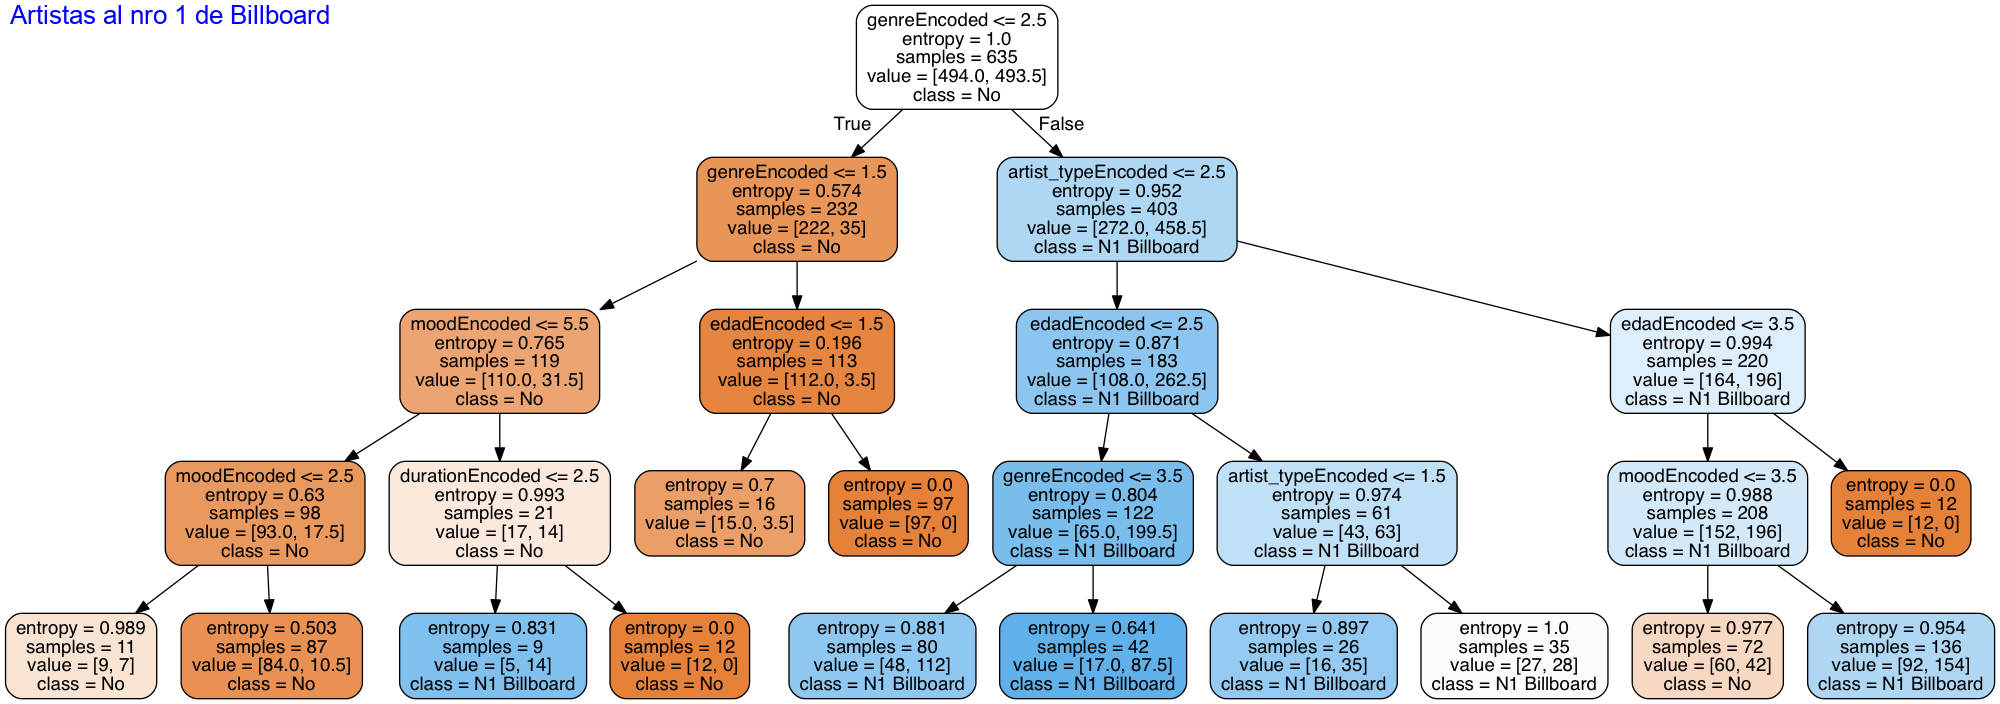
\includegraphics[width=0.7\textwidth]{capitulo4/arboldecision.png}
     \caption{Representación de un árbol de clasificación}
     \label{fig:arboldecision}
 \end{figure}


\subsection{Proceso de Construcción de un Árbol}
El proceso de generación de un árbol de decisión consta fundamentalmente de dos fases: la construcción del árbol y la poda del mismo.

\subsubsection{Fase de Construcción (Algoritmo Básico)}

El árbol se construye mediante \textbf{particionamiento recursivo}, un procedimiento descendente y voraz (\textit{greedy}) del tipo ``divide y vencerás''\cite{tema3_clasificacion}. Partiendo del nodo raíz, el algoritmo funciona de la siguiente manera:

\begin{itemize}

    \item Se parte del nodo raíz con todas las observaciones de entrenamiento.
    
    \item Si todas las observaciones del nodo son de la misma clase, o se cumple un criterio de parada, el nodo se convierte en hoja con la clase mayoritaria.
    
    \item En caso contrario, se evalúan las particiones posibles con cada variable predictora y se elige la que mayor reducción de impureza produce (Se calcula como la impureza del nodo padre menos la media ponderada de la de sus hijos).
    
    \item Se crea un nodo hijo por cada subconjunto resultante y se repite el proceso en cada uno.
\end{itemize}

Al ser voraz, el algoritmo elige la mejor partición local en cada paso, sin garantizar que el árbol resultante sea el óptimo global \cite{guion_arboles2024}.

\subsubsection{Criterios de Partición}
El método de selección para que la partición de los datos se haga de la mejor forma posible determina el rango óptimo para cada variable. Los atributos se seleccionan en base a una medida heurística o estadística. Sea un nodo $t$ y $p_j$ la proporción de observaciones de la clase $j$ ($j=1,\dots,J$). Las métricas más utilizadas son:

\begin{itemize}
    \item \textbf{Impureza de Gini:}  Es la medida de impureza en un nodo. Alcanza su mínimo (cero) cuando todos los casos del nodo corresponden a una sola categoría de destino  y alcanza su máximo, $1-1/J$, cuando las clases están equilibradas \cite{guion_arboles2024}.

     $G(t)=1-\sum_{j=1}^{J}p_j^2$
     
    \item \textbf{Entropía:} Vale $0$ para un nodo puro y su máximo es $\log_2 J$. ($0\log_2 0=0$) \cite{guion_arboles2024}.

    $H(t)=-\sum_{j=1}^{J}p_j\log_2 p_j$

\end{itemize}

\subsubsection{Criterios de Parada}

  El algoritmo debe saber cuándo terminar el particionamiento. Las condiciones naturales para detenerse son:

  \begin{itemize}
    \item Todos los ejemplos para un nodo dado pertenecen a la misma clase. 
    
    \item No quedan más atributos para seguir particionando; en este caso se utiliza el voto de la mayoría para clasificar el nodo hoja. 

    \item No quedan ejemplos.

    \item El número de observaciones es inferior a un mínimo establecido.

    \item Se alcanza una profundidad máxima.

    \item La mejora de impureza de la mejor partición es inferior a un umbral.

\end{itemize}

\subsection{Sobreajuste y Poda}

Un árbol que crece hasta tener hojas puras clasifica perfectamente los datos de entrenamiento, pero acaba modelando el ruido y generaliza mal: es el \textbf{sobreajuste}. Para controlarlo se utilizan dos estrategias:
\begin{itemize}

    \item \textbf{Prepoda}: Se detiene el crecimiento antes de que el árbol sea completo, fijando una profundidad máxima, un número mínimo de observaciones para dividir un nodo o por hoja, o una mejora mínima de la impureza. \cite{tema3_clasificacion}
    
    \item \textbf{Postpoda}: Se deja crecer el árbol completo y después se eliminan ramas. En el algoritmo CART, empleado en este trabajo mediante el paquete \textit{rpart} de R, la poda se basa en el criterio de coste-complejidad, controlado por el parámetro \textit{cp}: una división solo se conserva si reduce el error relativo del árbol en, al menos, ese valor. En este trabajo, \textit{cp} se fija antes de construir el árbol, por lo que, junto con \textit{minbucket}, actúa en la práctica como un criterio de parada durante el crecimiento. 
    
\end{itemize}


\subsection{Evaluación del modelo}
 
El error de un árbol debe estimarse con datos que no se hayan usado para construirlo. Para ello se emplea una partición \textbf{entrenamiento/prueba} (por ejemplo, 70\,\%/30\,\%, estratificada por clase) o \textbf{validación cruzada} de $k$ pliegues. Los resultados se resumen en la \textbf{matriz de confusión} (Tabla~\ref{tab:confusion}), a partir de la cual se calculan \cite{tema3_clasificacion}:
\[
\text{Exactitud}=\frac{VP+VN}{VP+VN+FP+FN},\quad
\text{Sensibilidad}=\frac{VP}{VP+FN},\quad
\]
\[
\text{Especificidad}=\frac{VN}{VN+FP},\quad
\text{Precisión}=\frac{VP}{VP+FP},\quad
\]
\[F_1=\frac{2\cdot\text{Precisión}\cdot\text{Sensibilidad}}{\text{Precisión}+\text{Sensibilidad}}.
\]
 
\begin{table}[ht]
\centering
\begin{tabular}{l|cc}
 & \textbf{Predicho positivo} & \textbf{Predicho negativo} \\ \hline
\textbf{Real positivo} & VP & FN \\
\textbf{Real negativo} & FP & VN \\
\end{tabular}
\caption{Matriz de confusión para un problema de clasificación binaria.}
\label{tab:confusion}
\end{table}
 
Cuando las clases están desbalanceadas, como ocurre con los tramos de alta siniestralidad, la exactitud es engañosa: un clasificador que prediga siempre la clase mayoritaria puede tener una exactitud alta y no detectar ningún tramo peligroso. En esos casos se recurre a la sensibilidad o el $F_1$  y se puede reequilibrar el conjunto de entrenamiento (ponderación de clases o remuestreo).

\vspace{0.5cm}

Cuando el árbol proporciona, además de la clase, una probabilidad de pertenecer a la clase positiva, puede utilizarse la \textbf{curva ROC}, que representa la sensibilidad frente a $1-\text{especificidad}$ para todos los umbrales de decisión posibles. El \textbf{área bajo la curva} (AUC) resume esta curva en un único valor: puede interpretarse como la probabilidad de que una observación positiva elegida al azar reciba una probabilidad mayor que una negativa elegida al azar. Vale $0.5$ para un clasificador que no discrimina mejor que el azar y $1$ para uno que separa perfectamente las clases y, al no depender de un umbral concreto, no se ve afectada por el desbalance de las clases \cite{tema3_clasificacion}.
 
\subsection{Uso del árbol y extracción de reglas}
 
Para clasificar una nueva observación se recorre el árbol desde la raíz, evaluando en cada nodo la prueba correspondiente, hasta llegar a una hoja, cuya clase es la predicción. Cada camino de la raíz a una hoja equivale a una regla de la forma
\[
\text{SI } (\text{Tipo de vía}=\text{Convencional}) \text{ Y } (\text{IMD Pesados}\leq c) \text{ ENTONCES } (\text{IP}=\text{Alto}),
\]
(ejemplo ilustrativo), de modo que un árbol puede convertirse en un Sistema Basado en Reglas (SBR).
 
\vspace{0.5cm}
 
Estas reglas guardan cierta analogía con las de asociación: la proporción de la clase mayoritaria en la hoja juega un papel similar a la confianza, y el número de observaciones de la hoja al del soporte. Sin embargo, difieren en aspectos esenciales: las reglas de un árbol forman una \textit{partición} (cada observación cae en una única hoja) y dependen del orden voraz de las divisiones, mientras que las reglas de Apriori pueden solaparse y se obtienen buscando exhaustivamente todas las combinaciones que superan los umbrales. Por ello ambas técnicas son complementarias.
 
\paragraph{Ventajas y limitaciones.} Los árboles son fáciles de interpretar, no requieren escalar las variables ni suponer una distribución concreta, admiten variables de distinto tipo y capturan interacciones y relaciones no lineales. Como limitaciones, son inestables (pequeños cambios en los datos pueden producir árboles muy distintos), tienden al sobreajuste si no se podan, realizan particiones paralelas a los ejes y, por sí solos, suelen tener menor capacidad predictiva que los métodos de conjunto (bosques aleatorios, \textit{boosting}), que combinan muchos árboles a costa de perder interpretabilidad \cite{tema2_clasificacion}.
 
%%%%%%%%%%%%%%%%%%%%%%%%%%% FIN CAP 4 %%%%%%%%%%%%%%%%%%%%%%%%%%%%%%%%%%%


%%%%%%%%%%%%%%% CAPÍTULO 5. Reglas de Asociación %%%%%%%%%%%%%%%%%%%%%%%
\setcounter{chapter}{5}
\chapter*{Capítulo 5 \\ \vspace{1cm} Aplicación de Reglas de Asociación}
\addcontentsline{toc}{chapter}{\protect\numberline{\thechapter} Aplicación de Reglas de Asociación}

\setcounter{section}{0}
\setcounter{subsection}{0}
\setcounter{figure}{0} \setcounter{table}{0}

En este capítulo se exponen los resultados obtenidos al aplicar técnicas de aprendizaje automático a los datos de siniestralidad vial. El objetivo principal es descubrir patrones de comportamiento ocultos (reglas de asociación) que nos permitan entender cómo interactúan las variables de tráfico y la infraestructura con la gravedad y frecuencia de los accidentes en la red de carreteras.

\section{Preparación de los Datos para el Modelado}

Aunque en el capítulo 3 se llevó a cabo un exhaustivo preprocesamiento de los datos de Accidentes y Tramos, la aplicación de algoritmos de extracción de reglas, como \textit{Apriori}, exige ciertas condiciones matemáticas. Para que el modelo sea eficiente en la búsqueda de patrones frecuentes, los datos deben estar en un formato categórico y transaccional. Por ello, se realizó un ajuste final del conjunto de datos, enfocado en los requisitos del algoritmo.

\subsection{Selección de Variables de Interés}

Incluir todas las variables disponibles en el algoritmo \textit{Apriori} podría generar una cantidad excesiva de reglas triviales o redundantes. Por ejemplo, al relacionar el número de accidentes con víctimas con el Índice de Peligrosidad, no se aporta conocimiento nuevo, ya que este último se calcula a partir del primero, existiendo una relación evidente de dependencia.

Para extraer conocimiento útil, se restringió el conjunto de datos a las variables más relevantes:
\begin{itemize}
    \item \textbf{Variables de contexto (Antecedentes potenciales):} Se seleccionaron \textit{Tipo de Vía} y las Intensidades Medias Diarias desglosadas (\textit{IMD\_Ligeros} e \textit{IMD\_Pesados}), ya que estos indicadores reflejan la exposición al riesgo y el desgaste de la infraestructura.
    
    \item \textbf{Variables de respuesta (Consecuentes potenciales):} Se eligieron el \textbf{Índice de Peligrosidad (IP)} y el \textbf{Índice de Mortalidad (IM)}, métricas que normalizan el riesgo al reducir el sesgo relacionado con la longitud del tramo y el tráfico diario.
\end{itemize}

La variable \textit{Tipo de Vía} contiene siete categorías: Autopista con peaje bonificado, Autopista de peaje, Autopista libre, Autopista libre de peaje para movimientos internos, Autovía, Carretera convencional y Carretera multicarril. Como en la base de 2024 las dos últimas aparecen con los nombres \textit{Convencional} y \textit{Multicarril}, se unificaron con estos nombres en ambos años.

\vspace{0.5cm}

Estas variables se aplicaron a las ocho bases de datos analizadas (tramos y accidentes, de los años 2023 y 2024, para el IP y para el IM). Cada una de ellas contiene las tres variables de contexto y únicamente el índice que le corresponde como variable respuesta, de manera que el IP y el IM nunca aparecen juntos en una misma base de datos.

\subsection{Discretización mediante Sextiles y Categorización Específica}

Dado que el algoritmo \textit{Apriori} no opera con variables de naturaleza numérica continua, resultó imprescindible proceder a la discretización de las variables seleccionadas relativas a la intensidad de tráfico (IMD) y a los índices de riesgo calculados (IP e IM), en cada una de las ocho bases de datos. 

\vspace{0.5cm}

En lugar de establecer umbrales de corte arbitrarios que pudieran sesgar el modelo dejando categorías vacías o sobrepobladas, se optó por una aproximación estadística robusta. Para conseguir un nivel de detalle óptimo sin sobrecargar computacionalmente el algoritmo, se decidió utilizar sextiles (seis divisiones) en lugar de los cuartiles tradicionales, aplicando una metodología dual adaptada a la naturaleza de cada variable:

\begin{itemize}
   
    \item \textbf{Variables de Exposición (IMD Ligeros y Pesados):} Se segmentaron usando sextiles, creando seis categorías que representan fielmente la distribución del tráfico: \textit{Muy Bajo, Bajo, Medio, Medio Alto, Alto} y \textit{Muy Alto}.
    
    \item \textbf{Variables de Riesgo (Índice de Peligrosidad e Índice de Mortalidad):} En el ámbito de la seguridad vial, la ausencia de siniestros no representa simplemente el extremo inferior de una métrica, sino el estado ideal de la infraestructura. Por consiguiente, se aisló el valor numérico exacto de cero en una categoría independiente y exclusiva (\textbf{Cero}). Únicamente los registros que sí presentaron siniestralidad (valores $> 0$) se sometieron a la partición por sextiles, adoptando la misma escala de seis niveles de intensidad.

\end{itemize}

Los puntos de corte de los sextiles se calcularon de forma independiente en cada una de las ocho bases de datos, por lo que las categorías son relativas a la distribución de cada una de ellas. La Tabla~\ref{tab:cortes_sextiles} recoge los valores que delimitan cada categoría y permite interpretar el significado de las etiquetas que aparecen en las reglas. Por ejemplo, en la base de tramos de 2023, un tramo con \textit{IMD Pesados Muy Bajo} es aquel que registra como máximo 120 vehículos pesados al día.

\begin{table}[H]
\centering
\small
\resizebox{\textwidth}{!}{%
\begin{tabular}{llrrrrrr}
\toprule
\textbf{Base de datos} & \textbf{Variable} & \textbf{Muy Bajo} & \textbf{Bajo} & \textbf{Medio} & \textbf{Medio Alto} & \textbf{Alto} & \textbf{Muy Alto} \\
\midrule
Tramos 2023 & IMD ligeros & $\leq 1136$ & $\leq 2651$ & $\leq 5315$ & $\leq 10394$ & $\leq 21566$ & $> 21566$ \\
 & IMD pesados & $\leq 120$ & $\leq 304$ & $\leq 596$ & $\leq 1380$ & $\leq 3534$ & $> 3534$ \\
 & IP & $\leq 4.45$ & $\leq 7.55$ & $\leq 12.26$ & $\leq 21.05$ & $\leq 42.17$ & $> 42.17$ \\
 & IM & $\leq 1.24$ & $\leq 2.29$ & $\leq 4.28$ & $\leq 8.29$ & $\leq 19.46$ & $> 19.46$ \\
\midrule
Tramos 2024 & IMD ligeros & $\leq 1150$ & $\leq 2640$ & $\leq 5347$ & $\leq 10748$ & $\leq 21695$ & $> 21695$ \\
 & IMD pesados & $\leq 120$ & $\leq 307$ & $\leq 609$ & $\leq 1396$ & $\leq 3578$ & $> 3578$ \\
 & IP & $\leq 4.34$ & $\leq 7.53$ & $\leq 12.33$ & $\leq 21.47$ & $\leq 43.18$ & $> 43.18$ \\
 & IM & $\leq 1.04$ & $\leq 1.87$ & $\leq 3.81$ & $\leq 7.61$ & $\leq 18.57$ & $> 18.57$ \\
\midrule
Accidentes 2023 & IMD ligeros & $\leq 5702$ & $\leq 13593$ & $\leq 24224$ & $\leq 42705$ & $\leq 78420$ & $> 78420$ \\
 & IMD pesados & $\leq 522$ & $\leq 1518$ & $\leq 3498$ & $\leq 5201$ & $\leq 9298$ & $> 9298$ \\
 & IP & $\leq 5.52$ & $\leq 8.32$ & $\leq 11.57$ & $\leq 18.45$ & $\leq 34.20$ & $> 34.20$ \\
 & IM & $\leq 0.65$ & $\leq 1.06$ & $\leq 1.64$ & $\leq 2.70$ & $\leq 7.73$ & $> 7.73$ \\
\midrule
Accidentes 2024 & IMD ligeros & $\leq 5639$ & $\leq 13702$ & $\leq 24526$ & $\leq 43415$ & $\leq 79423$ & $> 79423$ \\
 & IMD pesados & $\leq 545$ & $\leq 1574$ & $\leq 3363$ & $\leq 5233$ & $\leq 8758$ & $> 8758$ \\
 & IP & $\leq 5.36$ & $\leq 8.37$ & $\leq 12.03$ & $\leq 18.96$ & $\leq 34.28$ & $> 34.28$ \\
 & IM & $\leq 0.61$ & $\leq 0.96$ & $\leq 1.38$ & $\leq 2.32$ & $\leq 6.48$ & $> 6.48$ \\
\bottomrule
\end{tabular}}
\caption{Puntos de corte de los sextiles en cada base de datos. Las cinco primeras categorías incluyen el valor indicado y \textit{Muy Alto} agrupa los valores superiores. El IMD se expresa en vehículos/día, y el IP y el IM por cada $10^8$ vehículos$\cdot$km. En el IP y el IM los cortes corresponden únicamente a los valores mayores que cero, ya que el cero forma la categoría \textit{Cero}.}
\label{tab:cortes_sextiles}
\end{table}

Además, las bases de accidentes solo contienen puntos kilométricos con al menos un siniestro, de modo que en ellas la categoría \textit{Cero} únicamente aparece en el caso del IM. La Tabla~\ref{tab:recuento_sextiles} muestra el número de registros que queda en cada categoría de la variable respuesta. Se observa que los sextiles están equilibrados y que, en el IM, la categoría \textit{Cero} reúne en torno al 95\,\% de los tramos y más del 80\,\% de los puntos kilométricos, por lo que cada una de las seis categorías restantes agrupa pocos registros (unos 60 en las bases de tramos). Esto limita el número de reglas con IM que pueden alcanzar el soporte mínimo.

\begin{table}[H]
\centering
\small
\resizebox{\textwidth}{!}{%
\begin{tabular}{llrrrrrrrr}
\toprule
\textbf{Base de datos} & \textbf{Índice} & \textbf{Cero} & \textbf{Muy Bajo} & \textbf{Bajo} & \textbf{Medio} & \textbf{Medio Alto} & \textbf{Alto} & \textbf{Muy Alto} & \textbf{Total} \\
\midrule
Tramos 2023      & IP & 4097 & 528 & 527 & 528 & 527 & 527 & 528 & 7262 \\
Tramos 2023      & IM & 6901 & 61  & 60  & 60  & 60  & 60  & 60  & 7262 \\
Tramos 2024      & IP & 3985 & 544 & 544 & 544 & 543 & 544 & 544 & 7248 \\
Tramos 2024      & IM & 6879 & 62  & 61  & 62  & 61  & 61  & 62  & 7248 \\
\midrule
Accidentes 2023  & IP & --   & 1477 & 1474 & 1479 & 1472 & 1474 & 1475 & 8851 \\
Accidentes 2023  & IM & 7333 & 263 & 247 & 249 & 254 & 252 & 253 & 8851 \\
Accidentes 2024  & IP & --   & 1541 & 1529 & 1536 & 1533 & 1536 & 1532 & 9207 \\
Accidentes 2024  & IM & 7515 & 292 & 277 & 283 & 277 & 281 & 282 & 9207 \\
\bottomrule
\end{tabular}}
\caption{Número de registros de cada categoría de la variable respuesta en las ocho bases de datos. El guion indica que la categoría no existe en esa base.}
\label{tab:recuento_sextiles}
\end{table}


Esta segregación permite distinguir los tramos sin siniestralidad del resto y que las categorías superiores recojan únicamente los valores más altos del índice, que son los que se estudian en las reglas. Una vez transformadas las ocho bases de datos a este formato puramente categórico, se procedió a la ejecución del algoritmo de extracción de patrones.

\section{Ejecución del Algoritmo Apriori y Filtrado}

Una vez estructuradas las bases de datos en un formato puramente categórico, el siguiente paso consistió en la aplicación computacional del algoritmo \textit{Apriori} a cada una de las ocho bases de datos. Este modelo de aprendizaje automático iteró sobre los conjuntos de datos para descubrir todas aquellas combinaciones de variables que superasen los umbrales mínimos fijados.

\vspace{0.5cm}

Para garantizar que las reglas extraídas fuesen representativas y no simples coincidencias aleatorias, la configuración del algoritmo se fundamentó en tres parámetros críticos:
\begin{itemize}
    
    \item \textbf{Soporte mínimo (\textit{Support}):} Dado que los tramos con siniestralidad crítica (puntos negros) representan una minoría estadística frente a la totalidad de la red segura, este parámetro se ajustó deliberadamente a un umbral bajo ($0.002$ o $0.2\%$), el mismo en las ocho bases de datos para que los resultados sean comparables. Este valor equivale a unos 15 registros en las bases de tramos y a unos 18 en las de accidentes, lo que permite al modelo capturar patrones poco frecuentes sin apoyar ninguna regla en un número excesivamente reducido de casos.
    
    \item \textbf{Confianza mínima (\textit{Confidence}):} Se estableció en un valor muy bajo ($0.01$), que actúa únicamente como umbral técnico. No se emplearon umbrales más exigentes porque la confianza que puede alcanzar una regla depende de la frecuencia del consecuente en cada base de datos: las categorías \textit{Alto} y \textit{Muy Alto} del IP representan en torno al $7\%$ de los tramos cada una y las del IM menos del $1\%$, por lo que exigir una confianza más alta no habría proporcionado ninguna regla en alguna de las ocho bases. La relevancia de las reglas se evaluó, en su lugar, mediante el \textit{Lift}, que sí es comparable entre bases de datos.
    
    \item \textbf{Filtro de Antecedente y Consecuente (\textit{Appearance}):} Para filtrar únicamente el conocimiento útil y evitar la abundancia de reglas evidentes entre las propias variables de contexto, se parametrizó el algoritmo para que los antecedentes estuvieran formados exclusivamente por el tipo de vía y las intensidades de tráfico (ligeros y pesados), y para que extrajera únicamente aquellos patrones cuyo consecuente derivase en un Índice de Peligrosidad o de Mortalidad (según la base de datos) calificado como ``Alto'' o ``Muy Alto''.

\end{itemize}

Adicionalmente, debido al gran volumen de datos de tráfico y siniestralidad, la ejecución base del algoritmo tiende a generar inicialmente una cantidad considerable de reglas en bruto. Para destilar únicamente el conocimiento útil e identificar los verdaderos patrones de riesgo, se procedió a una fase de posprocesado computacional. 

\vspace{0.5cm}

En esta etapa de optimización, se conservaron únicamente las reglas con un valor de \textit{Lift} igual o superior a 1.5, es decir, aquellas en las que la probabilidad del consecuente es al menos un $50\%$ mayor que la esperada por azar, descartando así las asociaciones nulas, negativas o demasiado débiles. 

\vspace{0.5cm}

Seguidamente, mediante herramientas algorítmicas de poda, se identificaron y eliminaron las \textbf{reglas redundantes}, garantizando así la obtención de un subconjunto de patrones netamente accionables, listos para su interpretación en el ámbito de la seguridad vial.


\subsection{Resultados Extraídos: Patrones de Alta Peligrosidad y Mortalidad}

Tras aplicar los umbrales de soporte ($0.2\%$) y confianza ($0.01$), y conservar únicamente las reglas con \textit{Lift} igual o superior a 1.5 una vez eliminadas las redundantes, el algoritmo \textit{Apriori} logró aislar patrones en las ocho bases de datos. La Tabla~\ref{tab:resumen_reglas} recoge el número de reglas que quedan tras cada filtro, que se sitúa entre 12 y 44 reglas finales según la base de datos.

\begin{table}[H]
    \centering
    \caption{Número de reglas de asociación obtenidas en cada base de datos.}
    \vspace{0.3cm}
    \label{tab:resumen_reglas}
    \renewcommand{\arraystretch}{1.3}
    \begin{tabular}{lcccc}
        \toprule
        \textbf{Base de datos} & \textbf{Índice} & \textbf{Reglas en bruto} & \textbf{Con Lift $\geq 1.5$} & \textbf{Reglas finales} \\
        \midrule
        Tramos 2023     & IP & 94  & 30 & 26 \\
        Tramos 2023     & IM & 22  & 21 & 20 \\
        Tramos 2024     & IP & 96  & 47 & 36 \\
        Tramos 2024     & IM & 13  & 13 & 12 \\
        \midrule
        Accidentes 2023 & IP & 141 & 58 & 36 \\
        Accidentes 2023 & IM & 44  & 32 & 23 \\
        Accidentes 2024 & IP & 137 & 65 & 44 \\
        Accidentes 2024 & IM & 50  & 29 & 21 \\
        \bottomrule
    \end{tabular}
\end{table}

\vspace{0.5cm}

Para evidenciar el contraste en la granularidad de los datos, los hallazgos se han dividido en dos enfoques: el riesgo macroestructural (base de datos de Tramos) y el contexto situacional (base de datos de Accidentes Detallados). En ambas tablas se muestran, para cada índice y año, las cinco reglas con mayor \textit{Lift}.

\vspace{0.5cm}

En la \textbf{Tabla~\ref{tab:reglas_tramos}} se exponen las reglas más fuertes obtenidas al analizar la infraestructura agregada.

\begin{table}[H]
    \centering
    \caption{Top Reglas de Asociación - Enfoque Macroestructural (Tramos 2023 y 2024).}
    \vspace{0.3cm}
    \label{tab:reglas_tramos}
    \resizebox{\textwidth}{!}{
    \renewcommand{\arraystretch}{1.4}
    \begin{tabular}{cllcccc}
        \toprule
        \textbf{Año} & \textbf{Antecedentes (Contexto Vial)} & \textbf{Consecuente (Riesgo)} & \textbf{Soporte} & \textbf{Confianza} & \textbf{Lift} & \textbf{N.º reg.} \\
        \midrule
        2023 & Convencional + Ligeros (Medio Alto) + Pesados (Medio) & $\Rightarrow$ IP (Alto) & 0.0080 & 0.181 & 2.50 & 58 \\
        2023 & Convencional + Ligeros (Alto) + Pesados (Medio Alto) & $\Rightarrow$ IP (Alto) & 0.0036 & 0.176 & 2.42 & 26 \\
        2023 & Convencional + Pesados (Alto) & $\Rightarrow$ IP (Alto) & 0.0048 & 0.168 & 2.32 & 35 \\
        2023 & Convencional + Ligeros (Alto) & $\Rightarrow$ IP (Alto) & 0.0065 & 0.165 & 2.27 & 47 \\
        2023 & Convencional + Ligeros (Medio Alto) & $\Rightarrow$ IP (Alto) & 0.0146 & 0.156 & 2.15 & 106 \\
        \midrule
        2024 & Convencional + Ligeros (Alto) + Pesados (Alto) & $\Rightarrow$ IP (Alto) & 0.0021 & 0.224 & 2.98 & 15 \\
        2024 & Convencional + Ligeros (Alto) & $\Rightarrow$ IP (Alto) & 0.0069 & 0.179 & 2.39 & 50 \\
        2024 & Convencional + Pesados (Alto) & $\Rightarrow$ IP (Alto) & 0.0047 & 0.175 & 2.34 & 34 \\
        2024 & Convencional + Ligeros (Bajo) + Pesados (Muy Bajo) & $\Rightarrow$ IP (Muy Alto) & 0.0046 & 0.155 & 2.06 & 33 \\
        2024 & Ligeros (Bajo) + Pesados (Muy Bajo) & $\Rightarrow$ IP (Muy Alto) & 0.0047 & 0.153 & 2.04 & 34 \\
        \midrule
        2023 & Convencional + Ligeros (Medio Alto) & $\Rightarrow$ IM (Alto) & 0.0021 & 0.022 & 2.67 & 15 \\
        2023 & Convencional + Pesados (Medio Alto) & $\Rightarrow$ IM (Alto) & 0.0025 & 0.022 & 2.65 & 18 \\
        2023 & Pesados (Medio Alto) & $\Rightarrow$ IM (Alto) & 0.0028 & 0.017 & 2.00 & 20 \\
        2023 & Convencional + Ligeros (Medio) & $\Rightarrow$ IM (Muy Alto) & 0.0023 & 0.016 & 1.96 & 17 \\
        2023 & Convencional + Pesados (Medio) & $\Rightarrow$ IM (Muy Alto) & 0.0022 & 0.016 & 1.88 & 16 \\
        \midrule
        2024 & Convencional + Ligeros (Bajo) & $\Rightarrow$ IM (Muy Alto) & 0.0037 & 0.023 & 2.69 & 27 \\
        2024 & Ligeros (Bajo) & $\Rightarrow$ IM (Muy Alto) & 0.0037 & 0.022 & 2.61 & 27 \\
        2024 & Convencional + Ligeros (Medio) & $\Rightarrow$ IM (Alto) & 0.0028 & 0.019 & 2.28 & 20 \\
        2024 & Pesados (Medio Alto) & $\Rightarrow$ IM (Alto) & 0.0030 & 0.018 & 2.17 & 22 \\
        2024 & Pesados (Medio) & $\Rightarrow$ IM (Alto) & 0.0030 & 0.018 & 2.17 & 22 \\
        \bottomrule
    \end{tabular}
    }
\end{table}

\vspace{0.5cm}

Los valores de \textit{Lift} se sitúan aproximadamente entre 2 y 3, es decir, el consecuente es entre dos y tres veces más probable que en el conjunto de los tramos. Sin embargo, las confianzas son bajas: entre el $15\%$ y el $22\%$ para el IP y en torno al $2\%$ para el IM, lo cual es coherente con la escasa frecuencia de las categorías \textit{Alto} y \textit{Muy Alto} (aproximadamente un $7\%$ de los tramos en el IP y menos del $1\%$ en el IM). En el IP, las reglas de mayor \textit{Lift} son similares en ambos años: las carreteras convencionales con intensidades de tráfico, tanto ligero como pesado, de nivel medio a alto se asocian a un IP \textit{Alto}. 

\vspace{0.5cm}

También aparecen, con un \textit{Lift} menor, reglas de tráfico bajo o muy bajo asociadas a un IP \textit{Muy Alto}, como:
\[
\textit{Convencional + Ligeros (Bajo) + Pesados (Muy Bajo)} \Rightarrow \textit{IP (Muy Alto)}
\]
en 2024 (33 tramos y \textit{Lift} $2.06$), o:
\[
\textit{Convencional + Ligeros (Muy Bajo) + Pesados (Muy Bajo)} \Rightarrow \textit{IP (Muy Alto)}
\]
en 2023 (130 tramos, confianza $0.134$ y \textit{Lift} $1.85$). Las reglas del IM se apoyan en un número reducido de tramos (entre 15 y 27), por lo que deben interpretarse con prudencia.

\vspace{0.5cm}

Por otro lado, la \textbf{Tabla~\ref{tab:reglas_accidentes}} refleja el resultado de tratar cada punto kilométrico con siniestros de forma independiente.

\begin{table}[H]
    \centering
    \caption{Top Reglas de Asociación - Enfoque Situacional (Accidentes Detallados 2023 y 2024).}
    \vspace{0.3cm}
    \label{tab:reglas_accidentes}
    \resizebox{\textwidth}{!}{
    \renewcommand{\arraystretch}{1.4}
    \begin{tabular}{cllcccc}
        \toprule
        \textbf{Año} & \textbf{Antecedentes (Contexto Vial)} & \textbf{Consecuente (Riesgo)} & \textbf{Soporte} & \textbf{Confianza} & \textbf{Lift} & \textbf{N.º reg.} \\
        \midrule
        2023 & Autopista libre + Ligeros (Muy Alto) + Pesados (Medio) & $\Rightarrow$ IP (Alto) & 0.0026 & 1.000 & 6.00 & 23 \\
        2023 & Multicarril + Ligeros (Muy Bajo) & $\Rightarrow$ IP (Muy Alto) & 0.0032 & 0.933 & 5.60 & 28 \\
        2023 & Multicarril + Pesados (Muy Bajo) & $\Rightarrow$ IP (Muy Alto) & 0.0044 & 0.672 & 4.03 & 39 \\
        2023 & Convencional + Ligeros (Muy Bajo) + Pesados (Muy Bajo) & $\Rightarrow$ IP (Muy Alto) & 0.0691 & 0.591 & 3.55 & 612 \\
        2023 & Ligeros (Muy Bajo) + Pesados (Muy Bajo) & $\Rightarrow$ IP (Muy Alto) & 0.0732 & 0.591 & 3.55 & 648 \\
        \midrule
        2024 & Autopista libre + Ligeros (Muy Alto) + Pesados (Medio) & $\Rightarrow$ IP (Alto) & 0.0033 & 1.000 & 5.99 & 30 \\
        2024 & Multicarril + Ligeros (Alto) + Pesados (Bajo) & $\Rightarrow$ IP (Alto) & 0.0021 & 0.760 & 4.56 & 19 \\
        2024 & Multicarril + Ligeros (Medio Alto) + Pesados (Medio) & $\Rightarrow$ IP (Muy Alto) & 0.0037 & 0.642 & 3.86 & 34 \\
        2024 & Ligeros (Muy Alto) + Pesados (Medio) & $\Rightarrow$ IP (Alto) & 0.0056 & 0.619 & 3.71 & 52 \\
        2024 & Convencional + Ligeros (Muy Bajo) + Pesados (Muy Bajo) & $\Rightarrow$ IP (Muy Alto) & 0.0705 & 0.606 & 3.64 & 649 \\
        \midrule
        2023 & Convencional + Ligeros (Medio) + Pesados (Bajo) & $\Rightarrow$ IM (Alto) & 0.0025 & 0.125 & 4.39 & 22 \\
        2023 & Convencional + Ligeros (Muy Bajo) + Pesados (Muy Bajo) & $\Rightarrow$ IM (Muy Alto) & 0.0140 & 0.120 & 4.19 & 124 \\
        2023 & Convencional + Ligeros (Muy Bajo) & $\Rightarrow$ IM (Muy Alto) & 0.0179 & 0.115 & 4.03 & 158 \\
        2023 & Convencional + Ligeros (Bajo) + Pesados (Muy Bajo) & $\Rightarrow$ IM (Alto) & 0.0040 & 0.114 & 4.00 & 35 \\
        2023 & Ligeros (Muy Bajo) + Pesados (Muy Bajo) & $\Rightarrow$ IM (Muy Alto) & 0.0141 & 0.114 & 3.99 & 125 \\
        \midrule
        2024 & Convencional + Ligeros (Muy Bajo) + Pesados (Muy Bajo) & $\Rightarrow$ IM (Muy Alto) & 0.0133 & 0.114 & 3.72 & 122 \\
        2024 & Ligeros (Muy Bajo) + Pesados (Muy Bajo) & $\Rightarrow$ IM (Muy Alto) & 0.0135 & 0.112 & 3.64 & 124 \\
        2024 & Convencional + Ligeros (Muy Bajo) & $\Rightarrow$ IM (Muy Alto) & 0.0171 & 0.109 & 3.56 & 157 \\
        2024 & Ligeros (Muy Bajo) & $\Rightarrow$ IM (Muy Alto) & 0.0180 & 0.108 & 3.53 & 166 \\
        2024 & Convencional + Pesados (Muy Bajo) & $\Rightarrow$ IM (Muy Alto) & 0.0164 & 0.107 & 3.49 & 151 \\
        \bottomrule
    \end{tabular}
    }
\end{table}

\vspace{0.5cm}

Los valores de \textit{Lift} son mayores que en la base de Tramos (hasta $6.0$ en el IP y $4.4$ en el IM) y las confianzas alcanzan el $100\%$ en algunas reglas, aunque estas se apoyan en pocos registros (23 y 30 puntos kilométricos en las reglas de \textit{Autopista libre}). Estos valores no son directamente comparables con los de la tabla anterior: las bases de accidentes solo contienen puntos con al menos un siniestro, por lo que una parte importante de los tramos de poco tráfico, que no registraron accidentes, no aparece en ellas, y el índice de cada tramo se repite en todos sus puntos. 
Un ejemplo es la regla:
\[
\textit{Convencional + Ligeros (Muy Bajo) + Pesados (Muy Bajo)} \Rightarrow \textit{IP (Muy Alto)}
\] 
que en 2023 tiene una confianza de $0.134$ en la base de tramos y de $0.591$ en la de accidentes (con 612 registros, soporte $0.0691$ y \textit{Lift} $3.55$). En el IM, las reglas de mayor soporte se repiten en los dos años: las carreteras convencionales con tráfico ligero y pesado muy bajo se asocian a un IM \textit{Muy Alto} (124 registros en 2023 y 122 en 2024, con confianzas de $0.120$ y $0.114$).

%%%%%%%%%%%%%%%%%% FIN DE CAPÍTULO 5. Apriori  %%%%%%%%%%%%%%%%%

%%%%%%%%%%%%%%%%%%% CAPÍTULO 6. Árbol Decision %%%%%%%%%%%%%%%%%%%%%%%
\setcounter{chapter}{6}
\chapter*{Capítulo 6 \\ \vspace{1cm} Aplicación de Árboles de Clasificación}
\addcontentsline{toc}{chapter}{\protect\numberline{\thechapter}Aplicación de Árboles de Clasificación}
 
\setcounter{section}{0}
\setcounter{subsection}{0}
\setcounter{figure}{0}\setcounter{table}{0}
 
Como complemento a las reglas de asociación, se aplicaron árboles de clasificación con el fin de evaluar en qué medida las mismas variables de contexto (tipo de vía e intensidades de tráfico) permiten distinguir los tramos de mayor riesgo, y qué puntos de corte determina el propio algoritmo para separarlos. A diferencia de \textit{Apriori}, que busca asociaciones sin distinguir una variable de interés, un árbol de clasificación es un modelo supervisado y, por tanto, requiere definir una variable objetivo y evaluar su capacidad de predicción sobre datos no utilizados en su construcción.
 
\section{Preparación de los Datos para los Árboles}
 
\subsection{Variables predictoras}
 
Se emplearon las mismas variables de contexto que en las reglas de asociación: \textit{Tipo de Vía}, \textit{IMD Ligeros} e \textit{IMD Pesados}. En este caso las intensidades de tráfico no se discretizaron, sino que se mantuvieron como variables numéricas (vehículos/día), de modo que sea el propio algoritmo quien determine los puntos de corte más adecuados para separar los tramos. Esto evita la pérdida de información que supone agrupar los valores en sextiles y permite, además, comparar posteriormente los umbrales obtenidos con los de las reglas. El \textit{Tipo de Vía} se trató como variable categórica, con los mismos nombres unificados entre ambos años que en el apartado anterior. En las bases de Accidentes, las variables de contexto de cada punto kilométrico son las del tramo al que pertenece.
 
\vspace{0.5cm}
 
Se excluyeron las variables que intervienen directamente en el cálculo de los índices (número de accidentes, víctimas, fallecidos y longitud del tramo), así como las propias de cada punto kilométrico en las bases de Accidentes (número de accidentes, heridos y fallecidos), ya que el árbol podría reconstruir el índice a partir de ellas y los resultados carecerían de interés. Tampoco se incluyó la IMD total, por ser la suma de las intensidades de ligeros y pesados.
 
\subsection{Variable objetivo}
 
Los árboles de clasificación requieren una variable objetivo categórica, por lo que se definió una variable binaria basada en el mismo criterio que las categorías empleadas en las reglas de asociación. Un tramo se clasifica como de \textbf{riesgo alto} cuando su índice (IP o IM, según la base de datos) pertenece a las categorías \textit{Alto} o \textit{Muy Alto}, es decir, cuando supera el límite superior de la categoría \textit{Medio Alto} de la Tabla~\ref{tab:cortes_sextiles}.
 
\vspace{0.5cm}
 
En las bases de Tramos esto equivale a un IP mayor que $21.05$ en 2023 y $21.47$ en 2024, y a un IM mayor que $8.29$ en 2023 y $7.61$ en 2024. El resto de tramos, incluidos los que no registraron siniestros, forman la clase de riesgo no alto.
 
\vspace{0.5cm}
 
En las bases de Accidentes el límite se calcula de la misma forma, pero cambia lo que cuenta como registro. Cada fila de estas bases es un punto kilométrico con siniestros y lleva el índice del tramo al que pertenece, de modo que un tramo con varios puntos aparece repetido tantas veces como puntos tiene (en 2023 hay una media de 2.8 puntos por tramo, y el $45\%$ de los tramos tiene un único punto). Por ello, al calcular el valor que deja por debajo 4 de cada 6 registros, los tramos con más puntos pesan más y el límite resulta distinto al de las bases de Tramos: un IP mayor que $18.45$ en 2023 y $18.96$ en 2024, y un IM mayor que $2.70$ en 2023 y $2.32$ en 2024, que son los límites de la categoría \textit{Medio Alto} de las bases de Accidentes de la Tabla~\ref{tab:cortes_sextiles}. Se mantuvo este criterio para que la clase de riesgo alto coincida con las categorías \textit{Alto} y \textit{Muy Alto} empleadas en las reglas de asociación de estas mismas bases.
 
\vspace{0.5cm}
 
La consecuencia es que el \textit{riesgo alto} no significa exactamente lo mismo en ambos tipos de bases de datos: en las de Accidentes es relativo a la distribución de los puntos kilométricos con siniestros y, en el caso del IM, resulta más permisivo. Por ejemplo, en 2023 un tramo con un IM entre $2.70$ y $8.29$ es de riesgo alto en la base de Accidentes pero no en la de Tramos (212 tramos con siniestros superan el primer límite, frente a 120 que superan el segundo). Por este motivo, los resultados de ambos tipos de bases de datos no son directamente comparables.
 
\subsection{Distribución de las clases}
 
La Tabla~\ref{tab:clases_arboles} recoge el número de registros de cada base de datos (tramos en las bases de Tramos y puntos kilométricos en las de Accidentes) y la proporción de la clase de riesgo alto. En las bases de Tramos, aproximadamente un $15\%$ de los registros pertenece a esta clase en el IP y solo un $1.7\%$ en el IM (unos 120 tramos), mientras que en las de Accidentes representa el $33.3\%$ en el IP y entre el $5.7\%$ y el $6.1\%$ en el IM. Se trata, por tanto, de problemas con clases desbalanceadas, especialmente los del IM, lo que condiciona tanto el entrenamiento como la evaluación del modelo: como se explicó en el Capítulo~4, la exactitud no es una medida adecuada, ya que un clasificador que asignara siempre la clase mayoritaria obtendría una exactitud de en torno al $85\%$ en el IP de Tramos y al $98\%$ en el IM de Tramos (y de en torno al $67\%$ y al $94\%$ en el IP y el IM de Accidentes) sin detectar ningún registro de riesgo. Para que este desbalance no condicione también la construcción de los árboles, se aplicó un balanceo de las clases, que se describe en el apartado~\ref{sec:balanceo}.
 
\begin{table}[H]
\centering
\small
\begin{tabular}{llrrr}
\toprule
\textbf{Base de datos} & \textbf{Índice} & \textbf{Registros} & \textbf{Riesgo alto} & \textbf{\% riesgo alto} \\
\midrule
Tramos 2023     & IP & 7262 & 1055 & 14.5 \\
Tramos 2023     & IM & 7262 & 120  & 1.7  \\
Tramos 2024     & IP & 7248 & 1088 & 15.0 \\
Tramos 2024     & IM & 7248 & 123  & 1.7  \\
\midrule
Accidentes 2023 & IP & 8851 & 2949 & 33.3 \\
Accidentes 2023 & IM & 8851 & 505  & 5.7  \\
Accidentes 2024 & IP & 9207 & 3068 & 33.3 \\
Accidentes 2024 & IM & 9207 & 563  & 6.1  \\
\bottomrule
\end{tabular}
\caption{Número de registros y proporción de la clase de riesgo alto en cada base de datos.}
\label{tab:clases_arboles}
\end{table}
 
\subsection{Partición de los datos}
 
Para la búsqueda de los valores de los parámetros del árbol, cada base de datos se dividió de forma estratificada por clase en un $70\%$ de registros para entrenamiento y un $30\%$ para prueba, de manera que ambos conjuntos conservan la misma proporción de registros de riesgo alto. En las bases de Accidentes la partición se realizó por tramos: se seleccionó al azar el $70\%$ de los tramos de cada clase y todos sus puntos kilométricos pasaron al conjunto de entrenamiento, por lo que el porcentaje de puntos en cada conjunto es aproximadamente, y no exactamente, del $70\%$ y del $30\%$. La partición se realizó con una semilla fija para garantizar la reproducibilidad. Esta partición se utilizó únicamente para seleccionar los parámetros del árbol y evaluar su rendimiento: el conjunto de entrenamiento se empleó para elegir la combinación de parámetros, y el de prueba se reservó para una única evaluación final. Una vez fijados los parámetros, el árbol definitivo se construyó con la base de datos completa, como se describe en el apartado~\ref{sec:arboles_finales}. La Tabla~\ref{tab:particion_arboles} recoge el tamaño de ambos conjuntos en cada base de datos.
 
\begin{table}[H]
\centering
\small
\begin{tabular}{llrrrr}
\toprule
 &  & \multicolumn{2}{c}{\textbf{Entrenamiento}} & \multicolumn{2}{c}{\textbf{Prueba}} \\
\cmidrule(lr){3-4} \cmidrule(lr){5-6}
\textbf{Base de datos} & \textbf{Índice} & \textbf{Registros} & \textbf{Riesgo alto} & \textbf{Registros} & \textbf{Riesgo alto} \\
\midrule
Tramos 2023     & IP & 5083 & 738 & 2179 & 317 \\
Tramos 2023     & IM & 5083 & 84  & 2179 & 36  \\
Tramos 2024     & IP & 5074 & 762 & 2174 & 326 \\
Tramos 2024     & IM & 5074 & 86  & 2174 & 37  \\
\midrule
Accidentes 2023 & IP & 6270 & 2092 & 2581 & 857 \\
Accidentes 2023 & IM & 6347 & 354 & 2504 & 151 \\
Accidentes 2024 & IP & 6374 & 2090 & 2833 & 978 \\
Accidentes 2024 & IM & 6509 & 401 & 2698 & 162 \\
\bottomrule
\end{tabular}
\caption{Tamaño de los conjuntos de entrenamiento y prueba, y número de registros de riesgo alto en cada uno.}
\label{tab:particion_arboles}
\end{table}
 
Cabe destacar que en las bases del IM de Tramos el conjunto de prueba contiene únicamente 36 y 37 tramos de riesgo alto, por lo que las medidas de evaluación calculadas sobre ellos presentarán una variabilidad elevada y deben interpretarse con cautela.
 
\vspace{0.5cm}
 
Además, en las bases de Accidentes los registros de un mismo tramo no son independientes entre sí, por lo que sus resultados deben entenderse como los de un conjunto de tramos ponderados por el número de puntos kilométricos con siniestros que contienen.
 
\subsection{Balanceo de las clases}
\label{sec:balanceo}
 
Cuando una clase es mucho menos frecuente que la otra, el algoritmo de construcción del árbol tiende a favorecer la clase mayoritaria. Las divisiones se eligen según la reducción de la impureza de los nodos, y separar un grupo reducido de registros de riesgo alto apenas reduce la impureza del conjunto, por lo que el árbol puede no realizar ninguna división o clasificar todas sus hojas como riesgo no alto. En ese caso obtendría una exactitud elevada sin detectar ningún registro de riesgo alto. Como se indicó en el Capítulo~4, una forma de evitarlo es reequilibrar el conjunto de datos con el que se construye el árbol.
 
\vspace{0.5cm}
 
Existen distintas técnicas para ello. El \textbf{submuestreo} elimina registros de la clase mayoritaria hasta alcanzar la proporción deseada, pero supone descartar información: en el IM de Tramos habría que prescindir de la gran mayoría de los tramos de riesgo no alto. Otras técnicas generan registros sintéticos de la clase minoritaria a partir de los registros más parecidos entre sí, pero producen combinaciones de intensidades de tráfico que no corresponden a ningún tramo real y no están pensadas para variables categóricas como el tipo de vía. Por ello se empleó el \textbf{sobremuestreo aleatorio}: se conservan todos los registros originales y se añaden copias de registros de riesgo alto, elegidos al azar y con reemplazamiento (un mismo registro puede copiarse varias veces), hasta alcanzar la proporción deseada. De este modo no se elimina ningún registro y todos los que se añaden corresponden a tramos o puntos kilométricos reales.
 
\vspace{0.5cm}
 
Se fijó como objetivo una proporción de un $60\%$ de registros de riesgo no alto y un $40\%$ de riesgo alto. Con ella, la clase minoritaria pasa a tener un peso similar al de la mayoritaria sin llegar a igualarla, lo que limita el número de copias necesarias. Si $n_{\text{No}}$ y $n_{\text{Sí}}$ son el número de registros de riesgo no alto y de riesgo alto, el número de registros de riesgo alto tras el balanceo es
\begin{equation*}
n^{*}_{\text{Sí}} = n_{\text{No}} \cdot \frac{0.4}{0.6},
\end{equation*}
redondeado al entero más próximo, y se añaden $n^{*}_{\text{Sí}} - n_{\text{Sí}}$ copias. Por ejemplo, el conjunto de entrenamiento de Tramos IP 2023 contiene 4345 tramos de riesgo no alto y 738 de riesgo alto. Tras el balanceo pasa a tener 2897 registros de riesgo alto (los 738 originales y 2159 copias), con un total de 7242 registros, de los cuales el $60\%$ es de riesgo no alto y el $40\%$ de riesgo alto.
 
\vspace{0.5cm}
 
Las copias de registros de riesgo alto se añadieron únicamente a los datos con los que se construye cada árbol, y nunca a los datos con los que se evalúa, ya que estos deben conservar la proporción real de cada clase para que las medidas de evaluación reflejen el comportamiento del árbol sobre los datos tal y como son. En concreto, el balanceo se aplicó en tres momentos:

\begin{itemize}
    \item \textbf{En la búsqueda de parámetros} (apartado~\ref{sec:busqueda}). El procedimiento de validación cruzada es el mismo que sin balanceo, en cada turno se construye un árbol con cuatro de los cinco grupos y se evalúa con el grupo restante. La diferencia es que en cada turno, se separa primero el grupo de evaluación y después se añaden las copias a los cuatro grupos con los que se construye el árbol, mientras que el grupo de evaluación se mantiene sin copias. Si las copias se añadieran antes de separar los grupos, las copias de un mismo registro podrían quedar repartidas entre los datos de entrenamiento y los de prueba, de modo que el árbol se evaluaría con registros que ya ha visto y el AUC resultaría demasiado optimista.
    
    \item \textbf{En la evaluación final.} El árbol que se evalúa se construye con el conjunto de entrenamiento balanceado y se evalúa con el conjunto de prueba, sin copias.
    
    \item \textbf{En el árbol definitivo.} Se construyó con la base de datos completa balanceada, aunque en su representación se muestran los recuentos de los registros originales, sin las copias, como se explica en el apartado~\ref{sec:arboles_finales}.
\end{itemize}
 
El conjunto de prueba, los grupos de evaluación de la validación cruzada y los datos de 2024 empleados en la validación temporal conservan, por tanto, la proporción real de cada clase, de modo que las medidas de evaluación reflejan el comportamiento del árbol sobre los datos tal y como son. Las copias se sortearon con una semilla fija para garantizar la reproducibilidad. La Tabla~\ref{tab:balanceo_arboles} recoge el tamaño del conjunto de entrenamiento y de la base completa tras el balanceo.
 
\begin{table}[H]
\centering
\small
\setlength{\tabcolsep}{4pt}
\resizebox{\textwidth}{!}{%
\begin{tabular}{llrrrrrrrr}
\toprule
 &  & \multicolumn{4}{c}{\textbf{Entrenamiento balanceado}} & \multicolumn{4}{c}{\textbf{Base completa balanceada}} \\
\cmidrule(lr){3-6} \cmidrule(lr){7-10}
\textbf{Base de datos} & \textbf{Índice} & \textbf{No} & \textbf{Sí} & \textbf{Copias} & \textbf{Total} & \textbf{No} & \textbf{Sí} & \textbf{Copias} & \textbf{Total} \\
\midrule
Tramos 2023     & IP & 4345 & 2897 & 2159 & 7242       & 6207 & 4138 & 3083 & 10\,345 \\
Tramos 2023     & IM & 4999 & 3333 & 3249 & 8332       & 7142 & 4761 & 4641 & 11\,903 \\
Tramos 2024     & IP & 4312 & 2875 & 2113 & 7187       & 6160 & 4107 & 3019 & 10\,267 \\
Tramos 2024     & IM & 4988 & 3325 & 3239 & 8313       & 7125 & 4750 & 4627 & 11\,875 \\
\midrule
Accidentes 2023 & IP & 4178 & 2785 & 693  & 6963       & 5902 & 3935 & 986  & 9837 \\
Accidentes 2023 & IM & 5993 & 3995 & 3641 & 9988       & 8346 & 5564 & 5059 & 13\,910 \\
Accidentes 2024 & IP & 4284 & 2856 & 766  & 7140       & 6139 & 4093 & 1025 & 10\,232 \\
Accidentes 2024 & IM & 6108 & 4072 & 3671 & 10\,180    & 8644 & 5763 & 5200 & 14\,407 \\
\bottomrule
\end{tabular}}
\caption{Número de registros de riesgo no alto (No) y de riesgo alto (Sí) tras el balanceo 60/40, número de copias de registros de riesgo alto añadidas y total de registros, en el conjunto de entrenamiento y en la base de datos completa.}
\label{tab:balanceo_arboles}
\end{table}
 
En las bases del IM el número de copias es muy elevado: en las de Tramos cada tramo de riesgo alto aparece, por término medio, unas 40 veces, y en las de Accidentes, unas 10 u 11 veces, frente a unas 4 veces en el IP de Tramos y poco más de 1 en el IP de Accidentes. Las copias no aportan información nueva, sino que aumentan el peso de esos pocos registros, por lo que el árbol podría ajustarse a sus características particulares. Por ello sigue siendo necesario controlar el tamaño del árbol mediante los parámetros que se ajustan en el apartado~\ref{sec:busqueda}.
 
\vspace{0.5cm}
 
El balanceo modifica también el criterio con el que el árbol asigna la clase a cada hoja. Una hoja se clasifica como riesgo alto cuando, en los datos balanceados, contiene más registros de riesgo alto que de riesgo no alto, lo que, en los datos originales, equivale aproximadamente a que su proporción de riesgo alto supere los umbrales de la Tabla~\ref{tab:umbral_balanceo}. Por ejemplo, en Tramos IP 2023, donde el $14.5\%$ de los tramos es de riesgo alto, una hoja solo se clasifica como riesgo alto si esta proporción supera el $20.3\%$.

\begin{table}[H]
\centering
\small
\begin{tabular}{llcc}
\toprule
\textbf{Base de datos} & \textbf{Índice} & \textbf{\% riesgo alto real} & \textbf{Umbral de la hoja (\%)} \\
\midrule
Tramos 2023     & IP & 14.5 & 20.3 \\
Tramos 2023     & IM & 1.7  & 2.5  \\
Tramos 2024     & IP & 15.0 & 20.9 \\
Tramos 2024     & IM & 1.7  & 2.5  \\
\midrule
Accidentes 2023 & IP & 33.3 & 42.8 \\
Accidentes 2023 & IM & 5.7  & 8.3  \\
Accidentes 2024 & IP & 33.3 & 42.8 \\
Accidentes 2024 & IM & 6.1  & 8.9  \\
\bottomrule
\end{tabular}
\caption{Proporción real de riesgo alto en cada base de datos y proporción mínima de riesgo alto que debe tener una hoja para clasificarse como riesgo alto tras el balanceo 60/40.}
\label{tab:umbral_balanceo}
\end{table}
 
\section{Búsqueda de Valores de Parámetros}
\label{sec:busqueda}
 
Los resultados de un árbol de clasificación dependen de varios parámetros que controlan su tamaño. En este trabajo se ajustaron los dos que se consideraron más relevantes, empleando para ello únicamente el conjunto de entrenamiento de cada base de datos, de modo que el de prueba se mantiene sin utilizar hasta la evaluación final:
 
\begin{itemize}
    \item \textbf{cp} (parámetro de complejidad): una división solo se conserva si mejora el ajuste del árbol en, al menos, esa proporción, por lo que cuanto mayor es su valor más podado queda el árbol.
 
    \item \textbf{minbucket}: número mínimo de registros que debe contener cada hoja. Cuanto mayor es, menos hojas tiene el árbol.
\end{itemize}
 
Se probaron las 28 combinaciones resultantes de cruzar siete valores de cp ($0.001$, $0.0025$, $0.005$, $0.01$, $0.02$, $0.03$ y $0.05$) con cuatro de minbucket ($20$, $40$, $80$ y $120$). Para comparar las combinaciones se empleó validación cruzada repetida \cite{tema3_clasificacion}: el conjunto de entrenamiento se dividió aleatoriamente en 5 grupos y, por turnos, se construyó el árbol con cuatro de ellos y se midió su rendimiento con el restante. Este proceso se repitió con 5 repartos distintos, de modo que cada una de las 28 combinaciones se evaluó en 25 ocasiones (5 turnos en cada uno de los 5 repartos). Los grupos se formaron de manera estratificada, manteniendo en cada uno la proporción de la clase de riesgo alto y, en las bases de Accidentes, con tramos completos, por la misma razón que en la partición de los datos. En cada turno, los cuatro grupos de construcción se balancearon como se ha descrito en el apartado~\ref{sec:balanceo}, mientras que el grupo de evaluación se mantuvo sin balancear.
 
\vspace{0.5cm}
 
Como medida de rendimiento se utilizó el área bajo la curva ROC (AUC), que puede interpretarse como la probabilidad de que un registro de riesgo alto reciba del árbol una probabilidad mayor que uno de riesgo no alto. Vale $0.5$ cuando el modelo no distingue mejor que el azar y $1$ cuando separa las clases perfectamente. Se eligió frente a la exactitud porque no se ve afectada por el desbalance de las clases, tal y como se explicó en el Capítulo~4.
 
\vspace{0.5cm}
 
Para cada combinación se calculó la media y la desviación típica de los 25 valores del AUC, y se registró el número de hojas del árbol resultante al construirlo con todo el conjunto de entrenamiento balanceado. La Tabla~\ref{tab:busqueda_ip_2023} recoge, a modo de ejemplo, el resultado en la base de Tramos del IP de 2023; las tablas del resto de bases se encuentran en el Anexo.
 
\begin{table}[H]
\centering
\small
\setlength{\tabcolsep}{4pt}
\begin{tabular}{r|cccc}
\toprule
 & \multicolumn{4}{c}{\textbf{minbucket}} \\
\cmidrule(lr){2-5}
\textbf{cp} & \textbf{20} & \textbf{40} & \textbf{80} & \textbf{120} \\
\midrule
0.001 & \shortstack{0.6521~(0.0188)\\ 115 hojas} & \shortstack{0.6515~(0.0197)\\ 51 hojas} & \shortstack{0.6512~(0.0172)\\ 37 hojas} & \shortstack{0.6543~(0.0163)\\ 19 hojas} \\[4pt]
0.0025 & \shortstack{0.6441~(0.0226)\\ 35 hojas} & \shortstack{0.6530~(0.0169)\\ 43 hojas} & \shortstack{0.6530~(0.0146)\\ 28 hojas} & \shortstack{0.6559~(0.0208)\\ 20 hojas} \\[4pt]
0.005 & \shortstack{0.6528~(0.0187)\\ 17 hojas} & \shortstack{0.6532~(0.0225)\\ 19 hojas} & \shortstack{0.6509~(0.0203)\\ 14 hojas} & \shortstack{0.6525~(0.0164)\\ 16 hojas} \\[4pt]
0.01 & \shortstack{0.6553~(0.0191)\\ 4 hojas} & \shortstack{\textbf{0.6591}$^{*}$~\textbf{(0.0157)}\\ \textbf{4 hojas}} & \shortstack{0.6566~(0.0183)\\ 4 hojas} & \shortstack{0.6585~(0.0173)\\ 5 hojas} \\[4pt]
0.02 & \shortstack{0.6540~(0.0365)\\ 4 hojas} & \shortstack{0.6402~(0.0548)\\ 4 hojas} & \shortstack{0.6466~(0.0479)\\ 4 hojas} & \shortstack{0.6552~(0.0366)\\ 4 hojas} \\[4pt]
0.03 & \shortstack{0.5285~(0.0587)\\ 1 hoja} & \shortstack{0.5181~(0.0503)\\ 1 hoja} & \shortstack{0.5173~(0.0479)\\ 1 hoja} & \shortstack{0.5061~(0.0303)\\ 1 hoja} \\[4pt]
0.05 & \shortstack{0.5000~(0.0000)\\ 1 hoja} & \shortstack{0.5113~(0.0398)\\ 1 hoja} & \shortstack{0.5000~(0.0000)\\ 1 hoja} & \shortstack{0.5000~(0.0000)\\ 1 hoja} \\[4pt]
\bottomrule
\end{tabular}
\caption{Resultados de la búsqueda de parámetros con balanceo en la base de Tramos 2023, IP. En cada casilla se indica el AUC medio, entre paréntesis su desviación típica y, debajo, el número de hojas del árbol construido con todo el conjunto de entrenamiento balanceado. En negrita, la combinación elegida; con asterisco, la de mayor AUC medio.}
\label{tab:busqueda_ip_2023}
\end{table}
 
 
En esta base, las combinaciones con cp igual a $0.03$ o $0.05$ dan un árbol de una sola hoja, es decir, sin ninguna división: ninguna división mejora el ajuste del árbol en la proporción exigida. Un árbol así asigna la misma probabilidad a todos los tramos, por lo que su AUC es de $0.5$ o muy próximo a este valor.
 
\subsection{Criterio de selección}
 
Elegir directamente la combinación de mayor AUC medio no resulta adecuado, ya que las diferencias entre las mejores combinaciones suelen ser menores que la variabilidad del propio AUC. Por ejemplo, en Tramos IP 2024 (Tabla~\ref{tab:busqueda_ip_2024} del Anexo) el mejor valor ($0.6677$) corresponde a un árbol de 64 hojas, mientras que uno de solo 3 hojas obtiene $0.6619$: se diferencian en menos de $0.01$, frente a una desviación típica de $0.020$. Por ello se aplicó la \textbf{regla de una desviación típica}: entre las combinaciones cuyo AUC medio no es inferior al mejor menos una desviación típica de este, se eligió la que da el árbol más sencillo, es decir, con menor número de hojas. En caso de empate se eligió la de mayor AUC medio y, si este persistía, la de mayor poda (valores más altos de cp y de minbucket). De este modo se obtienen árboles más fáciles de interpretar y menos expuestos al sobreajuste.
 
\vspace{0.5cm}
 
A este criterio se añadieron dos condiciones. En primer lugar, se descartaron las combinaciones que dan un árbol de una sola hoja, ya que no realizan ninguna división y, por tanto, no permiten distinguir los registros de riesgo alto. En segundo lugar, se comprobó que el árbol definitivo, construido con la base de datos completa balanceada (apartado~\ref{sec:arboles_finales}), realizara al menos una división; si no lo hacía, la combinación se descartó y se pasó a la siguiente según el mismo criterio. Esta situación solo se dio en Tramos IM 2024: con la base completa balanceada, las combinaciones de 3 hojas, todas ellas con cp $=0.05$, y la de mayor AUC medio (cp $=0.03$ y minbucket $=80$, con 4 hojas) daban un árbol sin ninguna división, por lo que se eligió la siguiente combinación de 4 hojas, con cp $=0.02$ y minbucket $=80$. Esto se debe a que las copias de la base completa son distintas de las del conjunto de entrenamiento y, con valores altos de cp, la mejora que consigue la primera división puede quedar por debajo del valor exigido. La Tabla~\ref{tab:seleccion_parametros} resume el resultado en las ocho bases de datos.
 
\begin{table}[H]
\centering
\small
\resizebox{\textwidth}{!}{%
\begin{tabular}{llrrrrrrr}
\toprule
 &  & \multicolumn{2}{c}{\textbf{Mejor AUC}} & \multicolumn{5}{c}{\textbf{Combinación elegida}} \\
\cmidrule(lr){3-4} \cmidrule(lr){5-9}
\textbf{Base de datos} & \textbf{Índice} & \textbf{AUC} & \textbf{Hojas} & \textbf{cp} & \textbf{minbucket} & \textbf{AUC} & \textbf{Desv. típica} & \textbf{Hojas} \\
\midrule
Tramos 2023 & IP & 0.6591 & 4  & 0.01  & 40  & 0.6591 & 0.0157 & 4 \\
Tramos 2023 & IM & 0.6472 & 5  & 0.03  & 80  & 0.6472 & 0.0577 & 5 \\
Tramos 2024 & IP & 0.6677 & 64 & 0.01  & 120 & 0.6619 & 0.0136 & 3 \\
Tramos 2024 & IM & 0.6218 & 4  & 0.02  & 80  & 0.6208 & 0.0836 & 4 \\
\midrule
Accidentes 2023 & IP & 0.8092 & 12 & 0.005 & 80  & 0.8010 & 0.0311 & 2 \\
Accidentes 2023 & IM & 0.7587 & 4  & 0.05  & 120 & 0.7575 & 0.0623 & 3 \\
Accidentes 2024 & IP & 0.8273 & 6  & 0.005 & 120 & 0.8188 & 0.0321 & 2 \\
Accidentes 2024 & IM & 0.6681 & 2  & 0.05  & 20  & 0.6681 & 0.0474 & 2 \\
\bottomrule
\end{tabular}}
\caption{Mejor AUC medio de la búsqueda y combinación de parámetros elegida con la regla de una desviación típica en cada base de datos. El número de hojas corresponde al árbol construido con todo el conjunto de entrenamiento balanceado.}
\label{tab:seleccion_parametros}
\end{table}
 
En Tramos IP 2023, Tramos IM 2023 y Accidentes IM 2024, la combinación de mayor AUC medio es también la que da el árbol más sencillo, por lo que coincide con la elegida.
 
\subsection{Resultados de la búsqueda}
 
En todas las bases de datos los árboles elegidos, construidos con el conjunto de entrenamiento balanceado, son pequeños, de entre 2 y 5 hojas. Esto se debe a que complicar el árbol no mejora la capacidad de distinguir los registros de riesgo alto y, en las bases del IM, la empeora claramente. En el IM de Tramos de 2023, por ejemplo, el AUC medio pasa de $0.6472$ en el árbol de 5 hojas a valores de entre $0.50$ y $0.54$ en los de 55 a 104 hojas, es decir, prácticamente al nivel del azar: son árboles que se ajustan al ruido del conjunto de entrenamiento (sobreajuste). En estas bases el balanceo favorece este efecto, ya que cada tramo de riesgo alto aparece repetido unas 40 veces y un árbol grande puede dedicar hojas a aislar las copias de unos pocos tramos.
 
\vspace{0.5cm}
 
En las bases de Tramos, el AUC medio de los árboles elegidos es de en torno a $0.66$ en el IP y de entre $0.62$ y $0.65$ en el IM. Son valores bajos, que indican una capacidad de discriminación limitada y que son coherentes con los \textit{Lift} moderados de las reglas de asociación: el tipo de vía y la intensidad de tráfico explican solo una parte del riesgo. En el IM, además, la desviación típica entre repeticiones es elevada (entre $0.06$ y $0.08$), como consecuencia del escaso número de tramos de riesgo alto en el conjunto de entrenamiento (84 y 86): según qué tramos queden en cada grupo, y cuántas veces se copie cada uno, el árbol resultante cambia considerablemente.
 
\vspace{0.5cm}
 
En las bases de Accidentes el AUC es sensiblemente mayor, de alrededor de $0.80$ en el IP y de entre $0.67$ y $0.76$ en el IM. Estos valores no indican un modelo mejor, sino una consecuencia de la construcción de estas bases: solo contienen puntos kilométricos con al menos un siniestro, y el IP se calcula dividiendo entre la intensidad de tráfico y la longitud del tramo, de modo que, entre los tramos con accidentes, el tráfico, y con él el tipo de vía, determina en buena medida el valor del índice. Es significativo que en el IP de Accidentes el AUC apenas varía entre combinaciones (de $0.78$ a $0.81$ en 2023 y de $0.80$ a $0.83$ en 2024), lo que indica que una única división es suficiente; como se verá en el apartado siguiente, esta división se basa en el tipo de vía. En el IM de Accidentes la desviación típica es elevada (en torno a $0.05$ y $0.06$), por el reducido número de tramos de riesgo alto.
 
\section{Árboles finales y evaluación}
\label{sec:arboles_finales}
 
En cada base de datos se siguieron tres pasos. En primer lugar, se construyó un árbol con el conjunto de entrenamiento balanceado y la combinación de parámetros elegida, y se evaluó en el conjunto de prueba, sin balancear, mediante el AUC, con su intervalo de confianza al $95\%$, y la matriz de confusión. En segundo lugar, se construyó el \textbf{árbol definitivo} con la base de datos completa balanceada (todos los registros más las copias de riesgo alto) y la misma combinación de parámetros; es el árbol que se representa y se interpreta en cada apartado. Por último, en las bases de 2023 se aplicó el árbol definitivo a los datos de 2024, sin balancear, para comprobar si el patrón se mantiene de un año a otro (validación temporal).

\setcounter{subsection}{-1}
\subsection{El algoritmo de construcción de los árboles}
\label{sec:rpart}
 
Todos los árboles de este capítulo se construyeron en R con el paquete \texttt{rpart}, que implementa el algoritmo CART (\textit{Classification and Regression Trees}), y se representaron con el paquete \texttt{rpart.plot}. En este apartado se describe cómo aplica este algoritmo el proceso general de construcción presentado en el Capítulo~4 y qué parámetros se emplearon.
 
\subsubsection*{Divisiones binarias y criterio de partición}
 
CART construye árboles \textbf{binarios}: cada nodo se divide siempre en dos nodos hijos, de modo que una variable puede volver a utilizarse en divisiones posteriores, como ocurre con la intensidad de ligeros en varios de los árboles obtenidos. Para elegir cada división se empleó la \textbf{impureza de Gini} (Capítulo~4), que es el criterio por defecto: en cada nodo se prueban todas las divisiones posibles con cada variable predictora y se elige la que más reduce la impureza. La forma de generar las divisiones depende del tipo de variable:
 
\begin{itemize}
    \item \textbf{Variables numéricas} (IMD Ligeros e IMD Pesados). Se ordenan los valores distintos de la variable en el nodo y se prueba un punto de corte entre cada par de valores consecutivos, situado en el punto medio entre ambos. La división resultante es del tipo ``IMD Ligeros $< c$'' frente a ``IMD Ligeros $\geq c$''. Por este motivo, los puntos de corte de los árboles no coinciden necesariamente con un valor observado; en las figuras se han redondeado al entero más próximo.
    \item \textbf{Variables categóricas} (Tipo de Vía). La división agrupa las categorías en dos conjuntos, cada uno de los cuales va a un nodo hijo. Con una variable objetivo de dos clases, el algoritmo ordena las categorías según su proporción de riesgo alto en el nodo y solo prueba las divisiones que respetan ese orden, lo que garantiza encontrar la mejor agrupación sin probar todas las combinaciones posibles. Por ello, una misma división puede reunir tipos de vía muy distintos, como las carreteras convencionales y multicarril frente al resto.
\end{itemize}
 
\subsubsection*{Parámetros de control}
 
El crecimiento del árbol se controla mediante los parámetros de la función \texttt{rpart.control}. Los utilizados en este trabajo fueron los siguientes:
 
\begin{itemize}
    \item \textbf{cp}. El error de un árbol se mide como la proporción de registros mal clasificados, y cp se expresa en relación con el error del nodo raíz. Una división solo se conserva si, por sí sola o junto con las divisiones que cuelgan de ella, reduce el error del árbol en, al menos, cp veces el error del nodo raíz. En los datos balanceados el nodo raíz clasifica todos los registros como riesgo no alto, por lo que su error es del $40\%$. Con cp $=0.05$, por ejemplo, una división solo se conserva si reduce el error en $0.05 \cdot 0.40 = 0.02$, es decir, si clasifica correctamente al menos un $2\%$ más del total de registros. Esto explica que, con los valores más altos de cp, algunas combinaciones den árboles sin ninguna división (apartado~\ref{sec:busqueda}).
    \item \textbf{minbucket}. Número mínimo de registros en cada hoja. Al fijarlo, el algoritmo establece automáticamente el número mínimo de registros que debe tener un nodo para intentar dividirlo (\textit{minsplit}) en el triple de minbucket. En las bases balanceadas, estos mínimos incluyen las copias de los registros de riesgo alto.
    \item \textbf{xval}. Por defecto, \texttt{rpart} realiza una validación cruzada interna de 10 grupos para estimar el error de cada tamaño de árbol. Se fijó en $0$ para desactivarla, ya que la selección de parámetros se realizó con la validación cruzada repetida descrita en el apartado~\ref{sec:busqueda}. Además, la validación interna se aplicaría sobre los datos ya balanceados, de modo que las copias de un mismo registro podrían quedar a la vez en los grupos de construcción y de evaluación.
\end{itemize}
 
El resto de parámetros se mantuvieron en sus valores por defecto. Entre ellos, la profundidad máxima del árbol es de 30 niveles, un límite que no se alcanza con los valores de cp y minbucket empleados.
 
\subsubsection*{Clase y probabilidad de cada hoja}
 
Cada hoja se clasifica en la clase con más registros entre los datos con los que se construyó el árbol, por lo que, en los árboles con balanceo, se cuentan también las copias (apartado~\ref{sec:balanceo}). Además de la clase, el árbol asigna a cada hoja una probabilidad de riesgo alto, igual a la proporción de registros de riesgo alto que contiene. A todos los registros que llegan a una misma hoja se les asigna, por tanto, la misma probabilidad, y un árbol con pocas hojas solo produce unos pocos valores distintos.
 
\vspace{0.5cm}
 
Estas probabilidades son las que se utilizan para calcular la curva ROC y el AUC. En los árboles con balanceo están calculadas sobre los datos con copias, por lo que son más altas que la proporción real de riesgo alto de cada hoja y no deben interpretarse como probabilidades reales. Esto no afecta al AUC, que solo depende del orden en el que el árbol coloca los registros: una hoja con más riesgo alto que otra sigue recibiendo una probabilidad mayor. Por este motivo, en las figuras se muestra la proporción real de riesgo alto de cada hoja, calculada sobre los registros originales.
 
\vspace{0.5cm}
 
Por último, el algoritmo es determinista: con los mismos datos y los mismos parámetros produce siempre el mismo árbol. El azar interviene únicamente en la partición de los datos, en el reparto de los grupos de la validación cruzada y en el sorteo de las copias del balanceo, y en todos los casos se fijó una semilla para garantizar la reproducibilidad.

 
\subsection{Base de Datos de Tramos IP 2023}
 
El árbol construido con el conjunto de entrenamiento balanceado y la combinación elegida (cp $=0.01$ y minbucket $=40$) obtiene en el conjunto de prueba un AUC de $0.681$, con un intervalo de confianza al $95\%$ de $(0.654,\ 0.709)$. Este valor es algo superior al estimado mediante validación cruzada ($0.659$), lo que indica que el árbol no está sobreajustado, y el intervalo se sitúa claramente por encima de $0.5$, por lo que el modelo distingue los tramos de riesgo alto mejor que el azar. La Tabla~\ref{tab:confusion_ip_2023} recoge la matriz de confusión sobre el conjunto de prueba.
 
\begin{table}[H]
    \centering
    \vspace{0.3cm}
    \renewcommand{\arraystretch}{1.3}
    \begin{tabular}{lcc}
        \toprule
        & \multicolumn{2}{c}{\textbf{Real}} \\
        \cmidrule(lr){2-3}
        \textbf{Predicción} & \textbf{No} & \textbf{Sí} \\
        \midrule
        No & 1511 & 193 \\
        Sí & 351  & 124 \\
        \bottomrule
    \end{tabular}
    \caption{Matriz de confusión del árbol en el conjunto de prueba (Tramos IP 2023).}
    \label{tab:confusion_ip_2023}
\end{table}
 
\vspace{0.5cm}
 
A partir de ella se obtiene una sensibilidad de $0.391$, una especificidad de $0.811$, una precisión de $0.261$ y una exactitud de $0.750$. El árbol clasifica correctamente la mayoría de los tramos de riesgo no alto (1511 de 1862), pero solo detecta 124 de los 317 tramos de riesgo alto. Este comportamiento es consecuencia del criterio de asignación de clases que resulta del balanceo 60/40 (apartado~\ref{sec:balanceo}): una hoja solo se clasifica como riesgo alto cuando su proporción de tramos de riesgo alto supera claramente la de la base. La precisión es superior a la proporción de tramos de riesgo alto en el conjunto de prueba ($14.5\%$), ya que algo más de uno de cada cuatro tramos señalados como riesgo alto lo es realmente, y la exactitud no resulta una medida adecuada en este caso por el desbalance de las clases.
 
\vspace{0.5cm}
 
La Figura~\ref{fig:arbol_tramos_ip_2023} muestra el árbol definitivo, construido con la base de datos completa balanceada. Cada rama indica la condición que deben cumplir los tramos que la siguen. En cada nodo se muestra el número de tramos que contiene, el porcentaje que representan sobre el total y la proporción de tramos de riesgo alto, y en las hojas se indica además la clase asignada. Estos recuentos se calculan sobre la base de datos original, sin las copias añadidas en el balanceo, para que reflejen el número real de tramos y la proporción real de riesgo alto; la base balanceada solo se utiliza para construir el árbol. Por ello, el nodo raíz muestra los 7262 tramos de la base y su proporción real de riesgo alto ($14.5\%$), y no el $40\%$ de los datos balanceados. Lo mismo se aplica al resto de árboles de este capítulo.

\clearpage 
\begin{sidewaysfigure}
    \centering
    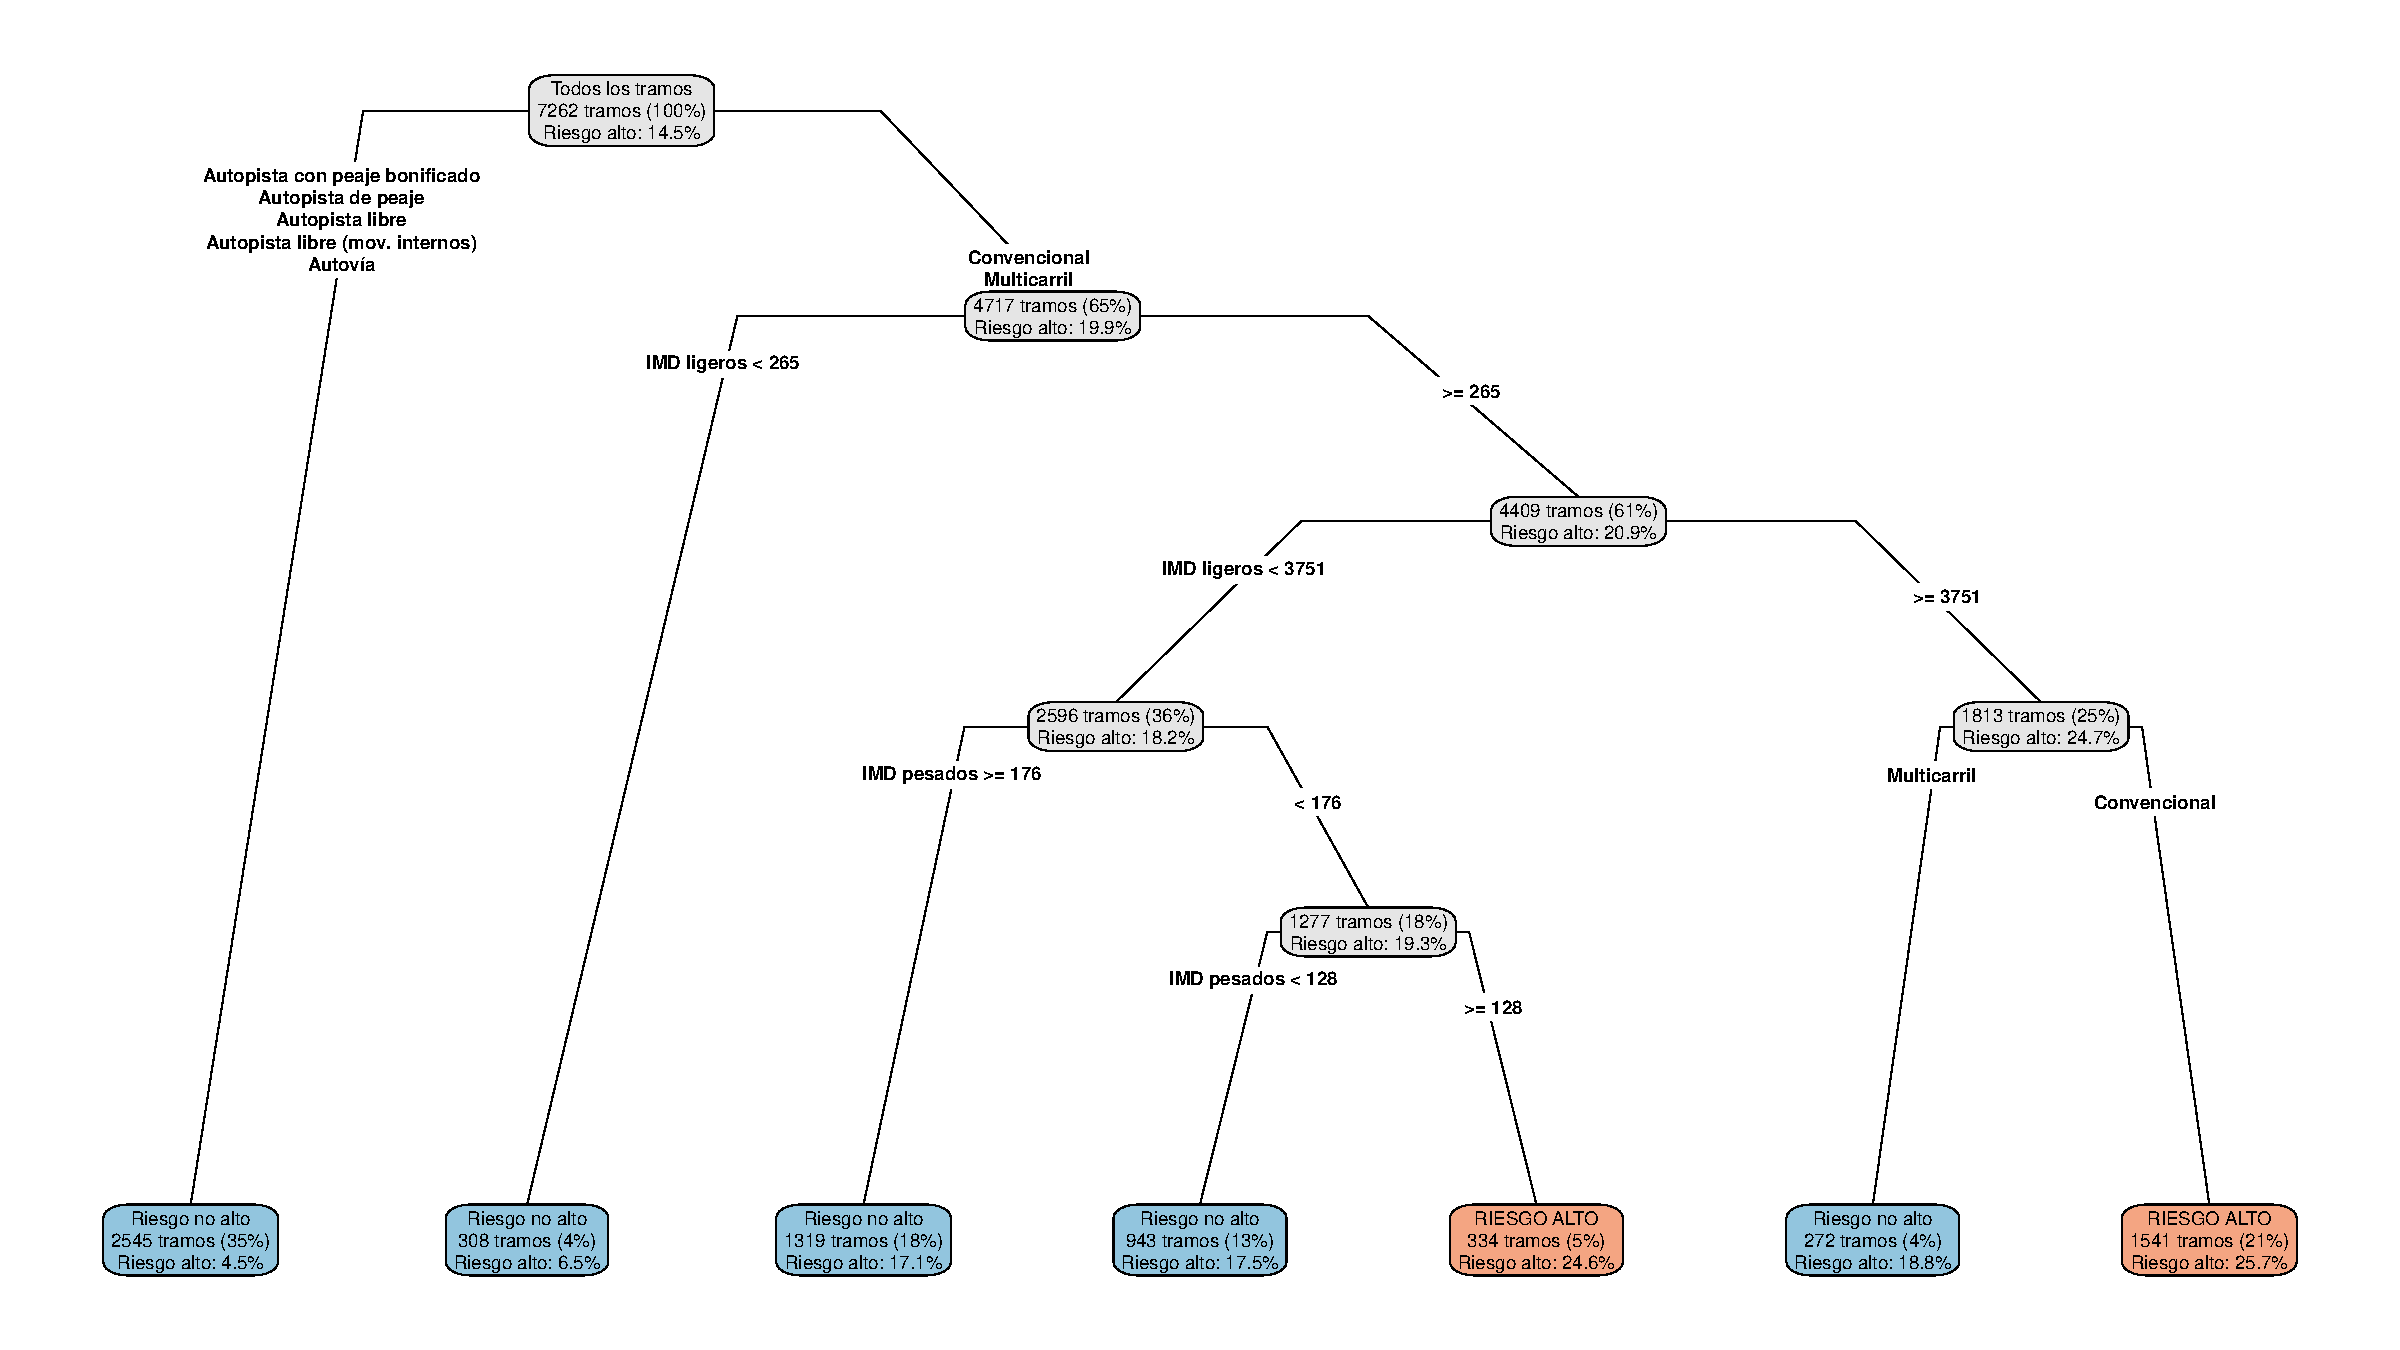
\includegraphics[width=\textwidth]{arboles6.3/arboltrip23.pdf}
    \caption{Árbol de clasificación definitivo para la base de Tramos IP 2023.}
    \label{fig:arbol_tramos_ip_2023}
\end{sidewaysfigure}
\clearpage

El árbol tiene siete hojas y su primera división se basa en el tipo de vía:
 
\begin{itemize}
    \item Las autopistas y autovías (2545 tramos, el $35\%$ del total) se clasifican como riesgo no alto. En ellas, solo el $4.5\%$ de los tramos es de riesgo alto.
    \item Las carreteras convencionales y multicarril (4717 tramos, el $65\%$) se dividen a su vez según la intensidad de tráfico ligero. Los tramos con menos de 265 vehículos ligeros diarios (308 tramos, el $4\%$) se clasifican como riesgo no alto, con un $6.5\%$ de tramos de riesgo alto.
    \item Entre los tramos con 3751 o más vehículos ligeros diarios (1813 tramos, el $25\%$), las carreteras convencionales (1541 tramos, el $21\%$) se clasifican como riesgo alto, con una proporción real del $25.7\%$, y las multicarril (272 tramos, el $4\%$) como riesgo no alto, con un $18.8\%$.
    \item Los tramos con entre 265 y 3751 vehículos ligeros diarios (2596 tramos, el $36\%$) se dividen según la intensidad de pesados. Se clasifican como riesgo no alto los que tienen 176 o más pesados diarios (1319 tramos, $17.1\%$) y los que tienen menos de 128 (943 tramos, $17.5\%$), mientras que los que tienen entre 128 y 176 pesados se clasifican como riesgo alto (334 tramos, $24.6\%$).
\end{itemize}
 
En la práctica, el árbol separa las vías de alta capacidad de las convencionales y multicarril, y asigna el mayor riesgo a las carreteras convencionales con más tráfico ligero. La hoja comprendida entre 128 y 176 pesados recoge un intervalo muy estrecho de intensidades y las diferencias entre las hojas de esa rama son pequeñas (del $17.1\%$ al $24.6\%$), por lo que no debe interpretarse como un patrón general.
 
\vspace{0.5cm}
 
Por último, al aplicar este árbol a los datos de 2024 se obtiene un AUC de $0.673$, muy similar al obtenido en el conjunto de prueba de 2023. El patrón aprendido se mantiene, por tanto, de un año a otro.
 
\subsection{Base de Datos de Tramos IM 2023}
 
El árbol construido con el conjunto de entrenamiento balanceado y la combinación elegida (cp $=0.03$ y minbucket $=80$) obtiene en el conjunto de prueba un AUC de $0.707$, con un intervalo de confianza al $95\%$ de $(0.635,\ 0.780)$. Este valor es superior al estimado mediante validación cruzada ($0.647$) y el intervalo se sitúa por encima de $0.5$, aunque es bastante más amplio que en el IP, ya que el conjunto de prueba solo contiene 36 tramos de riesgo alto. La Tabla~\ref{tab:confusion_im_2023} recoge la matriz de confusión sobre el conjunto de prueba.
 
\begin{table}[H]
    \centering
    \vspace{0.3cm}
    \renewcommand{\arraystretch}{1.3}
    \begin{tabular}{lcc}
        \toprule
        & \multicolumn{2}{c}{\textbf{Real}} \\
        \cmidrule(lr){2-3}
        \textbf{Predicción} & \textbf{No} & \textbf{Sí} \\
        \midrule
        No & 1640 & 17 \\
        Sí & 503  & 19 \\
        \bottomrule
    \end{tabular}
    \caption{Matriz de confusión del árbol en el conjunto de prueba (Tramos IM 2023).}
    \label{tab:confusion_im_2023}
\end{table}
 
\vspace{0.5cm}
 
A partir de ella se obtiene una sensibilidad de $0.528$, una especificidad de $0.765$, una precisión de $0.036$ y una exactitud de $0.761$. El árbol detecta algo más de la mitad de los tramos de riesgo alto (19 de 36) y clasifica como tales a 503 de los 2143 tramos restantes. La precisión duplica la proporción de tramos de riesgo alto en el conjunto de prueba ($1.7\%$), pero es muy baja en términos absolutos: de cada 27 tramos señalados como riesgo alto, aproximadamente uno lo es realmente.
 
\vspace{0.5cm}
 
La Figura~\ref{fig:arbol_tramos_im_2023} muestra el árbol definitivo, construido con la base de datos completa balanceada.

\clearpage

\begin{sidewaysfigure}
    \centering
    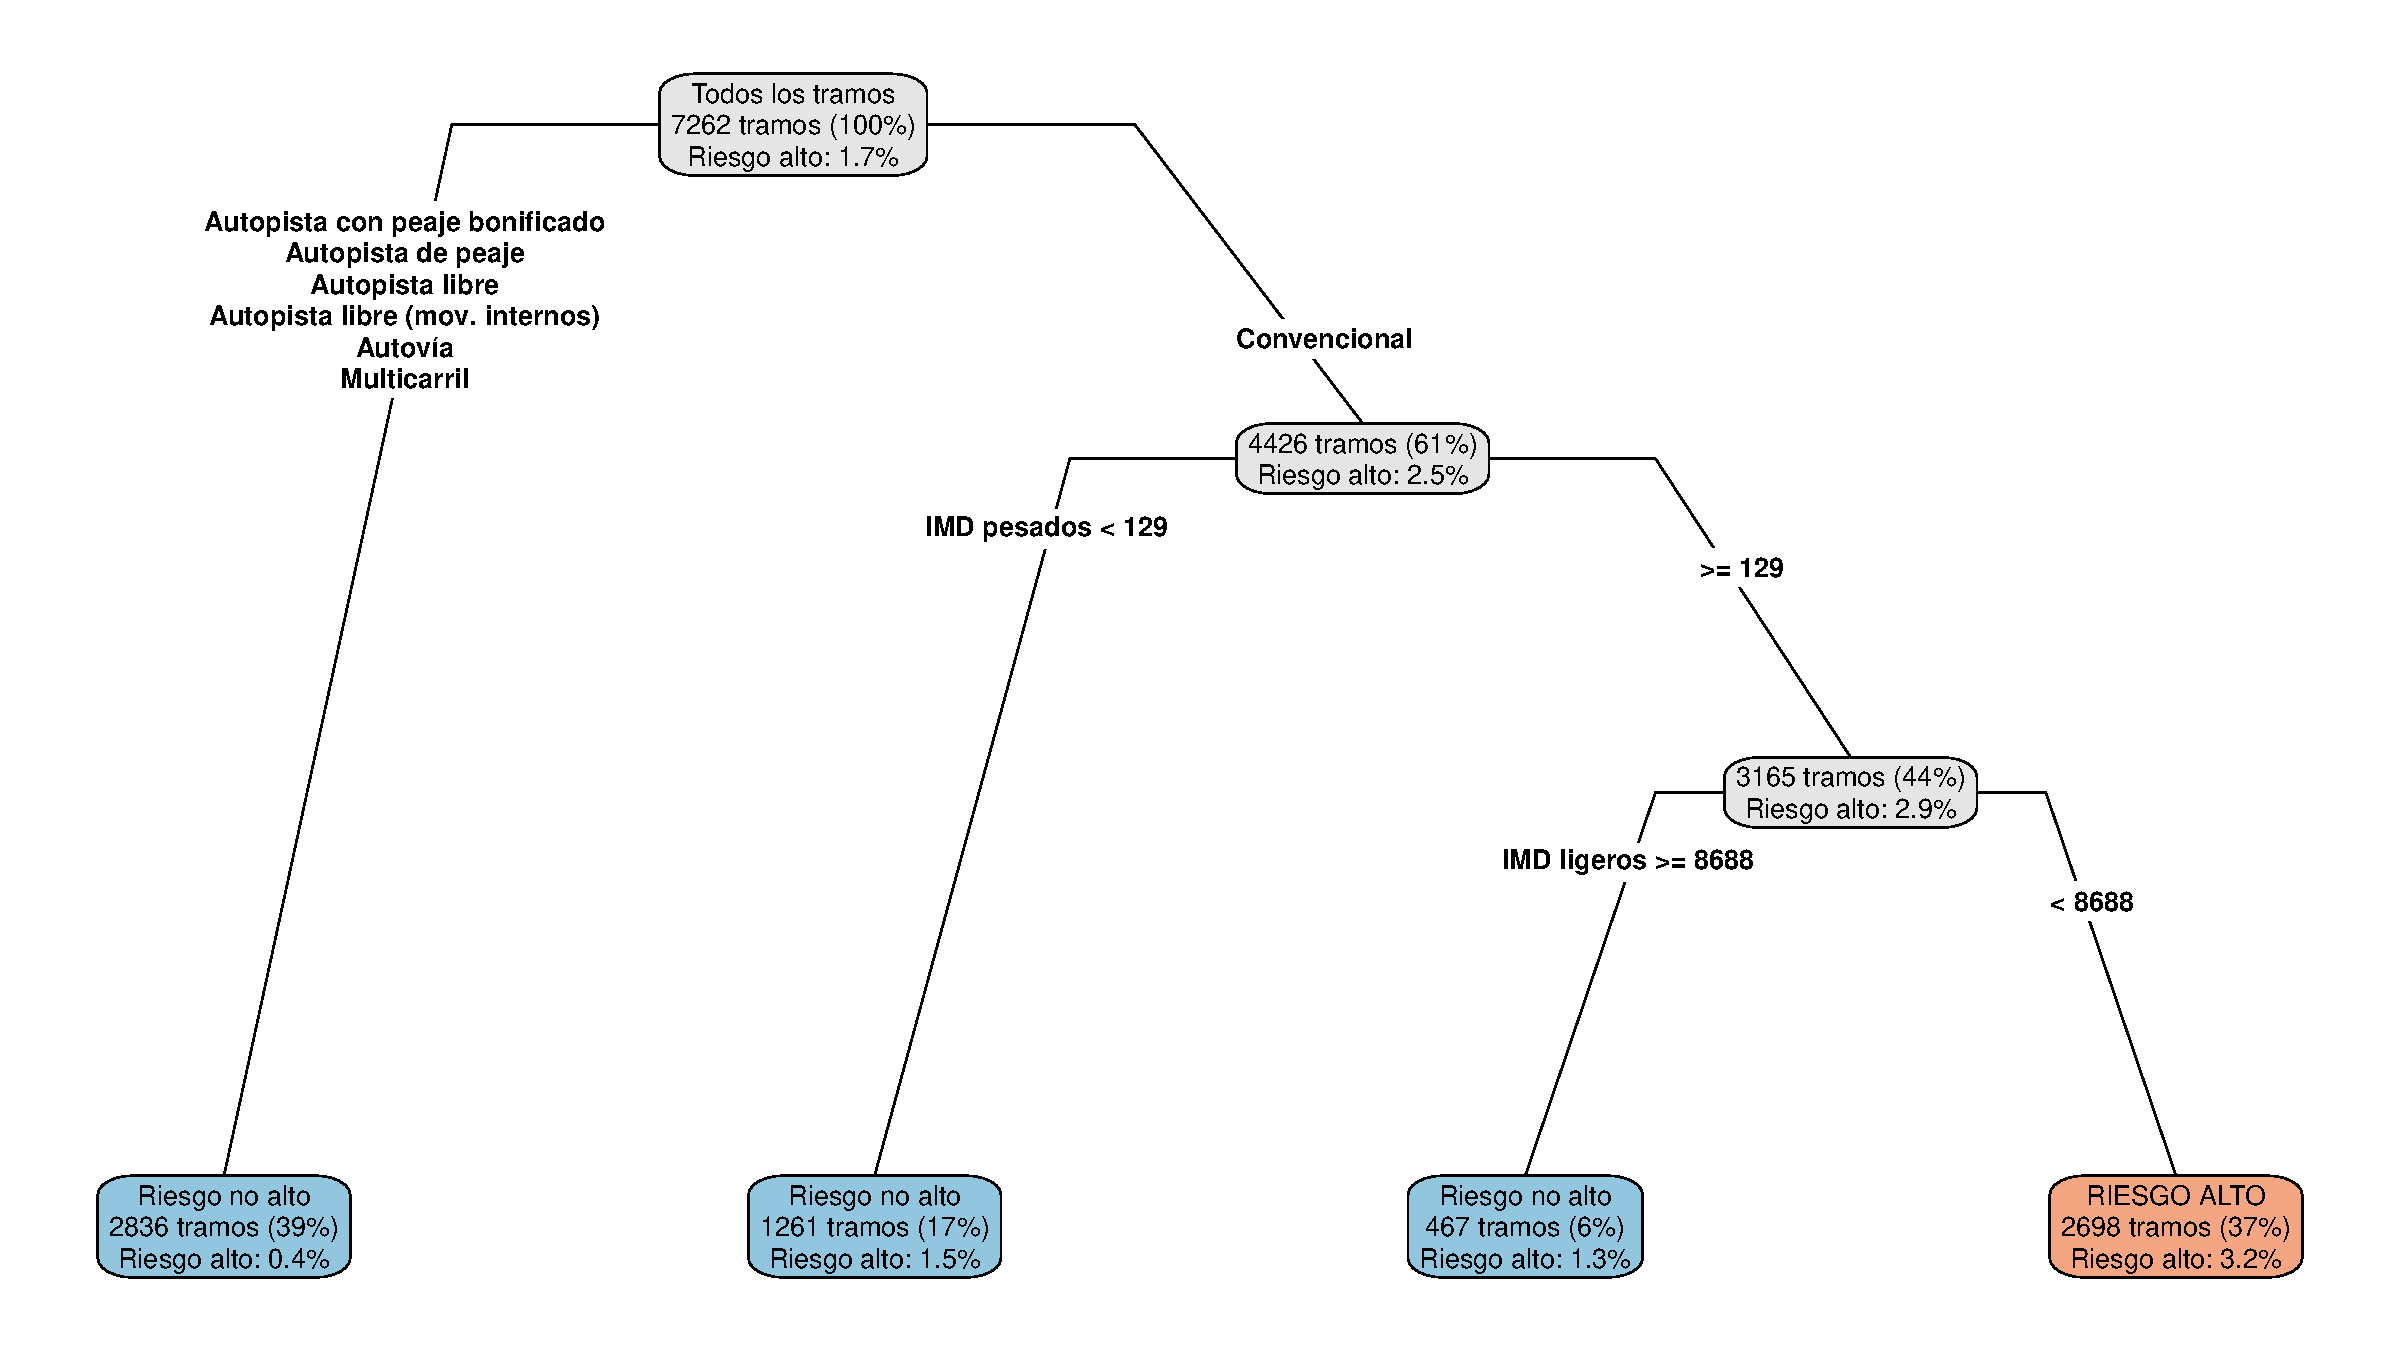
\includegraphics[width=\textwidth]{arboles6.3/arboltrim23.pdf}
    \caption{Árbol de clasificación definitivo para la base de Tramos IM 2023.}
    \label{fig:arbol_tramos_im_2023}
\end{sidewaysfigure}
\clearpage

El árbol tiene cuatro hojas y su primera división se basa en el tipo de vía:
 
\begin{itemize}
    \item El resto de tipos de vía, incluidas en este caso las carreteras multicarril (2836 tramos, el $39\%$), se clasifican como riesgo no alto, con solo un $0.4\%$ de tramos de riesgo alto.
    \item Las carreteras convencionales (4426 tramos, el $61\%$), con un $2.5\%$ de riesgo alto, se dividen según la intensidad de pesados. Los tramos con menos de 129 pesados diarios (1261 tramos, el $17\%$) se clasifican como riesgo no alto ($1.5\%$).
    \item Entre los tramos con 129 o más pesados (3165 tramos, el $44\%$), los que tienen 8688 o más vehículos ligeros diarios (467 tramos, el $6\%$) se clasifican como riesgo no alto ($1.3\%$), y los que tienen menos de 8688 (2698 tramos, el $37\%$), como riesgo alto, con una proporción real del $3.2\%$.
\end{itemize}
 
El riesgo alto de mortalidad se concentra así en las carreteras convencionales con un tráfico de pesados no muy bajo y un tráfico ligero moderado, cuya proporción de riesgo alto es unas ocho veces la del resto de tipos de vía, aunque en todas las hojas es muy reducida debido a la escasa frecuencia de la clase. A diferencia del IP, las carreteras multicarril se agrupan aquí con las vías de alta capacidad.
 
\vspace{0.5cm}
 
Por último, al aplicar este árbol a los datos de 2024, el AUC desciende a $0.637$, por lo que el patrón del IM resulta menos estable entre años que el del IP.
 
\subsection{Base de Datos de Tramos IP 2024}
 
El árbol construido con el conjunto de entrenamiento balanceado y la combinación elegida (cp $=0.01$ y minbucket $=120$) obtiene en el conjunto de prueba un AUC de $0.672$, con un intervalo de confianza al $95\%$ de $(0.650,\ 0.693)$. Este valor está en línea con el estimado mediante validación cruzada ($0.662$), por lo que el árbol no está sobreajustado, y el intervalo se sitúa claramente por encima de $0.5$. La Tabla~\ref{tab:confusion_ip_2024} recoge la matriz de confusión sobre el conjunto de prueba.
 
\begin{table}[H]
    \centering
    \vspace{0.3cm}
    \renewcommand{\arraystretch}{1.3}
    \begin{tabular}{lcc}
        \toprule
        & \multicolumn{2}{c}{\textbf{Real}} \\
        \cmidrule(lr){2-3}
        \textbf{Predicción} & \textbf{No} & \textbf{Sí} \\
        \midrule
        No & 878 & 45  \\
        Sí & 970 & 281 \\
        \bottomrule
    \end{tabular}
    \caption{Matriz de confusión del árbol en el conjunto de prueba (Tramos IP 2024).}
    \label{tab:confusion_ip_2024}
\end{table}
 
\vspace{0.5cm}
 
A partir de ella se obtiene una sensibilidad de $0.862$, una especificidad de $0.475$, una precisión de $0.225$ y una exactitud de $0.533$. A diferencia de 2023, el árbol identifica la mayoría de los tramos de riesgo alto (281 de 326), a costa de clasificar como tales a más de la mitad de los tramos que no lo son (970 de 1848). La precisión es superior a la proporción de tramos de riesgo alto en el conjunto de prueba ($15.0\%$).
 
\vspace{0.5cm}
 
La Figura~\ref{fig:arbol_tramos_ip_2024} muestra el árbol definitivo, construido con la base de datos completa balanceada.

\clearpage
\begin{sidewaysfigure}
    \centering
    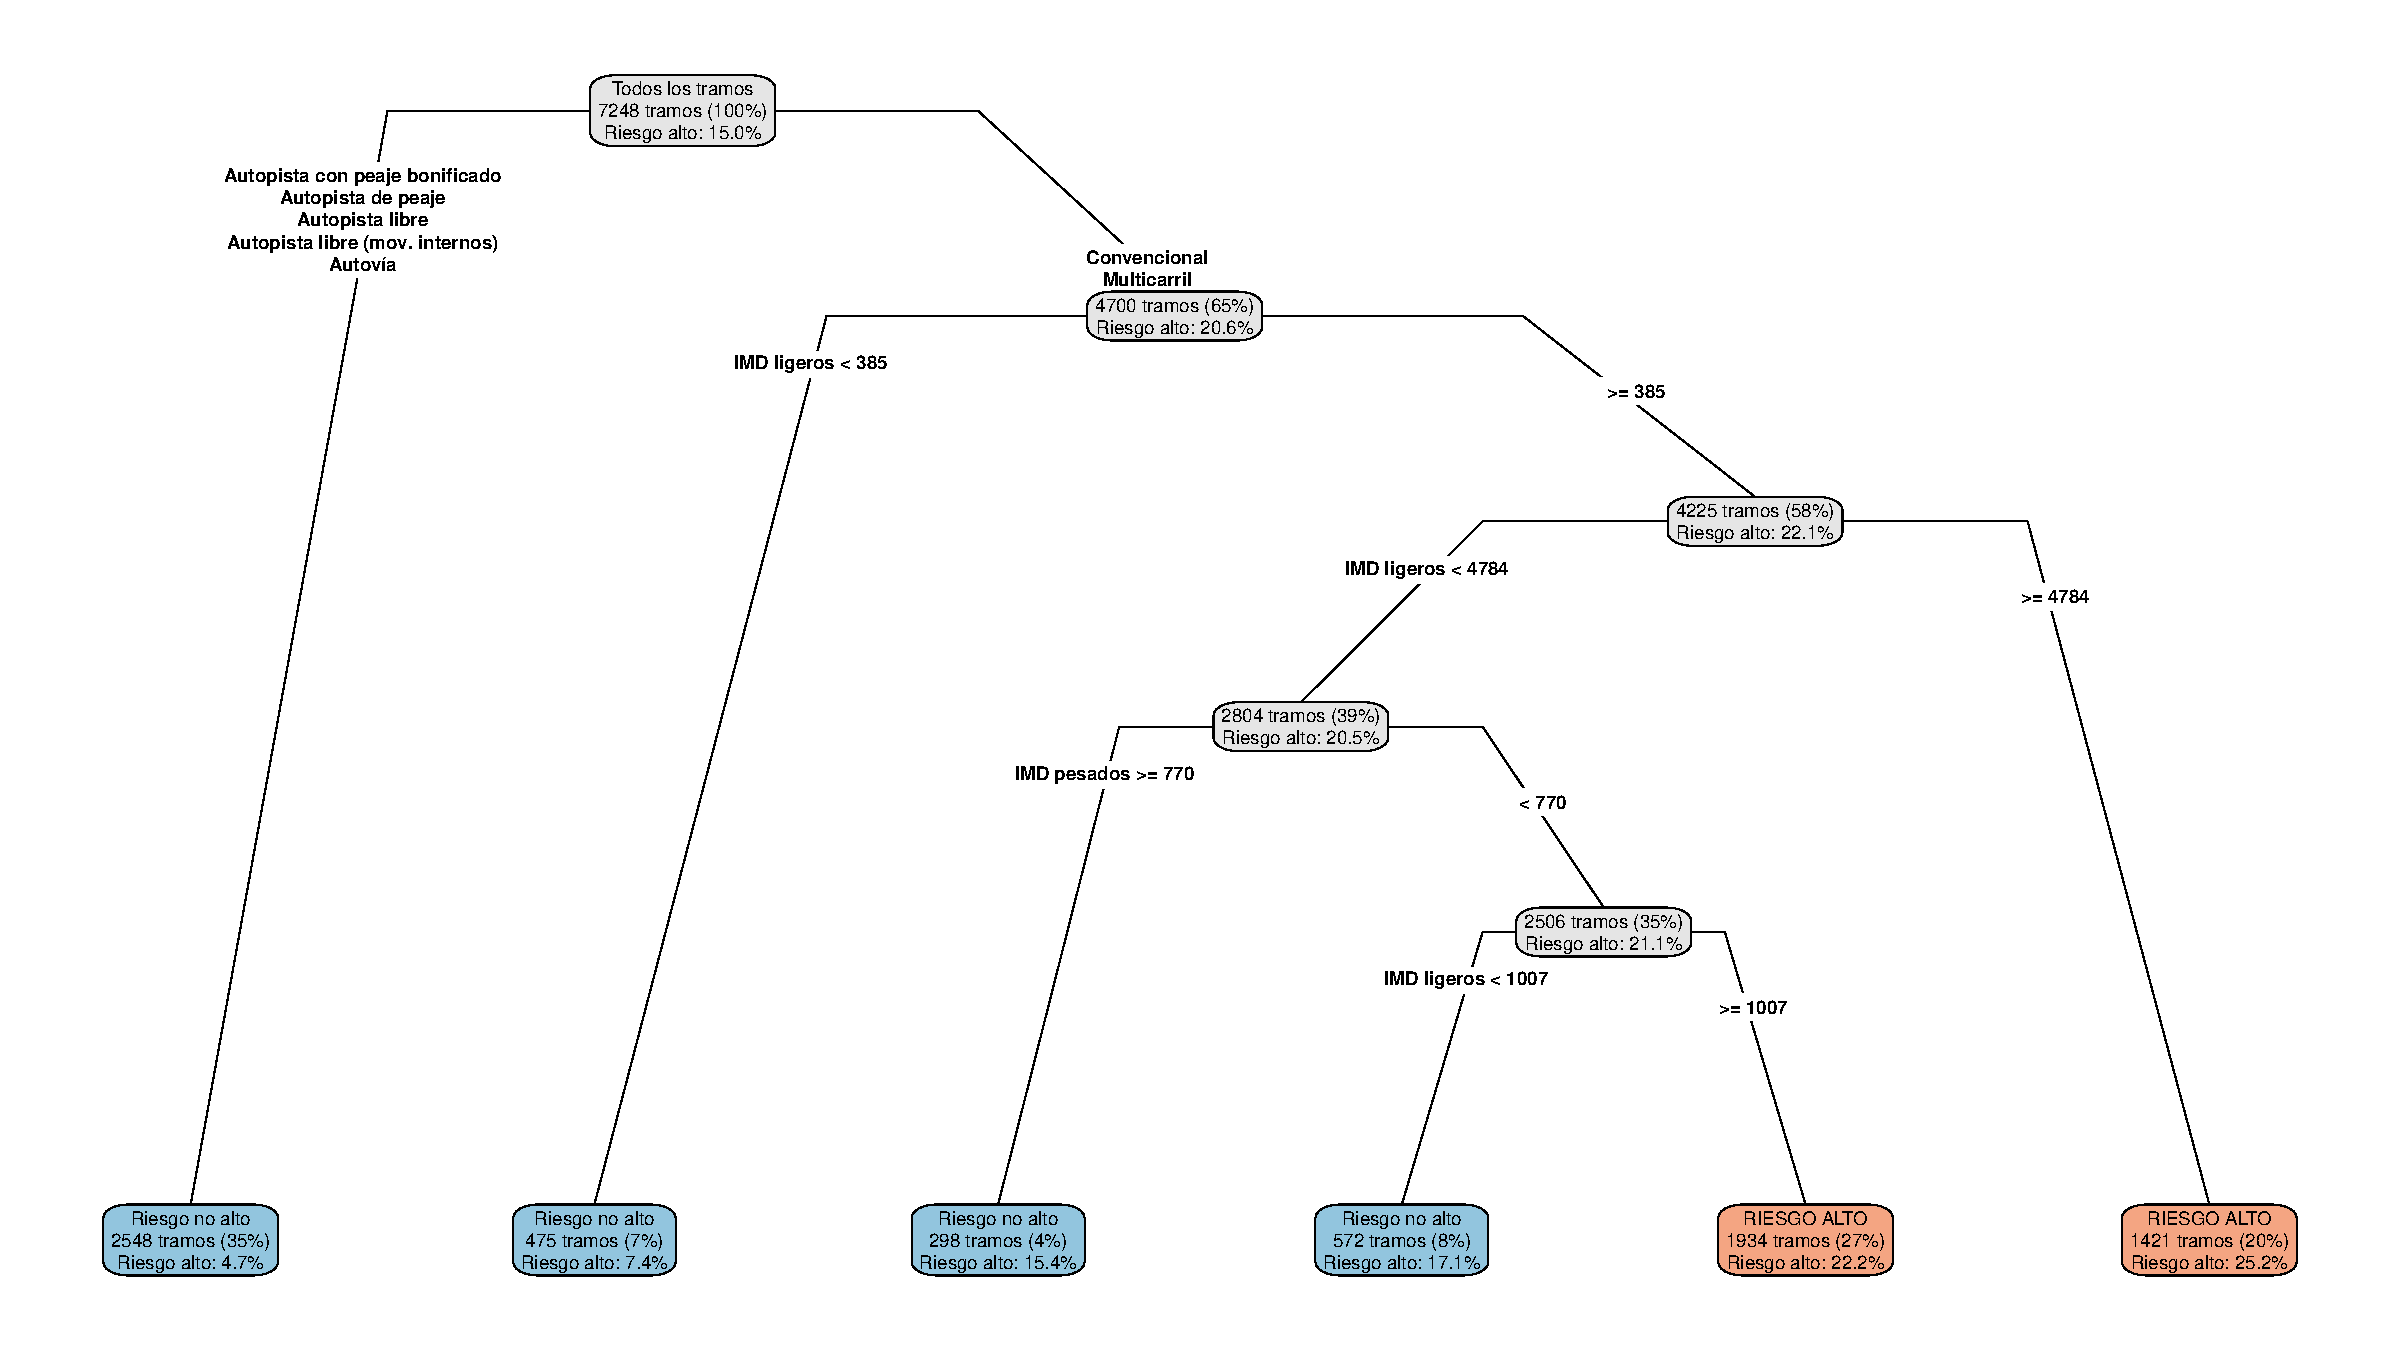
\includegraphics[width=\textwidth]{arboles6.3/arboltrip24.pdf}
    \caption{Árbol de clasificación definitivo para la base de Tramos IP 2024.}
    \label{fig:arbol_tramos_ip_2024}
\end{sidewaysfigure}
\clearpage

El árbol tiene seis hojas, frente a las tres del árbol construido con el conjunto de entrenamiento, ya que al disponer de más registros se conservan más divisiones con los mismos parámetros. Su estructura es similar a la de 2023:
 
\begin{itemize}
    \item Las autopistas y autovías (2548 tramos, el $35\%$) se clasifican como riesgo no alto, con un $4.7\%$ de tramos de riesgo alto.
    \item Las carreteras convencionales y multicarril (4700 tramos, el $65\%$) se dividen según la intensidad de tráfico ligero. Los tramos con menos de 385 vehículos ligeros diarios (475 tramos, el $7\%$) se clasifican como riesgo no alto ($7.4\%$), y los que tienen 4784 o más (1421 tramos, el $20\%$), como riesgo alto, con una proporción real del $25.2\%$.
    \item Los tramos con entre 385 y 4784 vehículos ligeros diarios (2804 tramos, el $39\%$) se dividen según la intensidad de pesados y de ligeros. Se clasifican como riesgo no alto los que tienen 770 o más pesados diarios (298 tramos, $15.4\%$) y, entre los demás, los que tienen menos de 1007 ligeros (572 tramos, $17.1\%$), mientras que los que tienen 1007 o más ligeros se clasifican como riesgo alto (1934 tramos, el $27\%$, con un $22.2\%$).
\end{itemize}
 
Como en 2023, las vías de alta capacidad presentan el riesgo más bajo y, dentro de las carreteras convencionales y multicarril, el riesgo aumenta con la intensidad de tráfico ligero. Los puntos de corte cambian respecto a 2023 (de 265 a 385 vehículos ligeros diarios en la primera división por tráfico), y en este año las carreteras multicarril no se separan de las convencionales.
 
\subsection{Base de Datos de Tramos IM 2024}
 
El árbol construido con el conjunto de entrenamiento balanceado y la combinación elegida (cp $=0.02$ y minbucket $=80$) obtiene en el conjunto de prueba un AUC de $0.598$, con un intervalo de confianza al $95\%$ de $(0.513,\ 0.682)$. Es el valor más bajo de los ocho árboles e inferior al estimado mediante validación cruzada ($0.621$), y el límite inferior del intervalo queda muy próximo a $0.5$, por lo que la capacidad del árbol para distinguir los tramos de riesgo alto es limitada. La Tabla~\ref{tab:confusion_im_2024} recoge la matriz de confusión sobre el conjunto de prueba.
 
\begin{table}[H]
    \centering
    \vspace{0.3cm}
    \renewcommand{\arraystretch}{1.3}
    \begin{tabular}{lcc}
        \toprule
        & \multicolumn{2}{c}{\textbf{Real}} \\
        \cmidrule(lr){2-3}
        \textbf{Predicción} & \textbf{No} & \textbf{Sí} \\
        \midrule
        No & 1287 & 16 \\
        Sí & 850  & 21 \\
        \bottomrule
    \end{tabular}
    \caption{Matriz de confusión del árbol en el conjunto de prueba (Tramos IM 2024).}
    \label{tab:confusion_im_2024}
\end{table}
 
\vspace{0.5cm}
 
A partir de ella se obtiene una sensibilidad de $0.568$, una especificidad de $0.602$, una precisión de $0.024$ y una exactitud de $0.602$. De los 37 tramos de riesgo alto del conjunto de prueba, el árbol detecta 21, mientras que clasifica como riesgo alto a 850 de los 2137 tramos que no lo son. La precisión apenas supera la proporción de tramos de riesgo alto en el conjunto de prueba ($1.7\%$).
 
\vspace{0.5cm}
 
La Figura~\ref{fig:arbol_tramos_im_2024} muestra el árbol definitivo, construido con la base de datos completa balanceada.

\clearpage
\begin{sidewaysfigure}
    \centering
    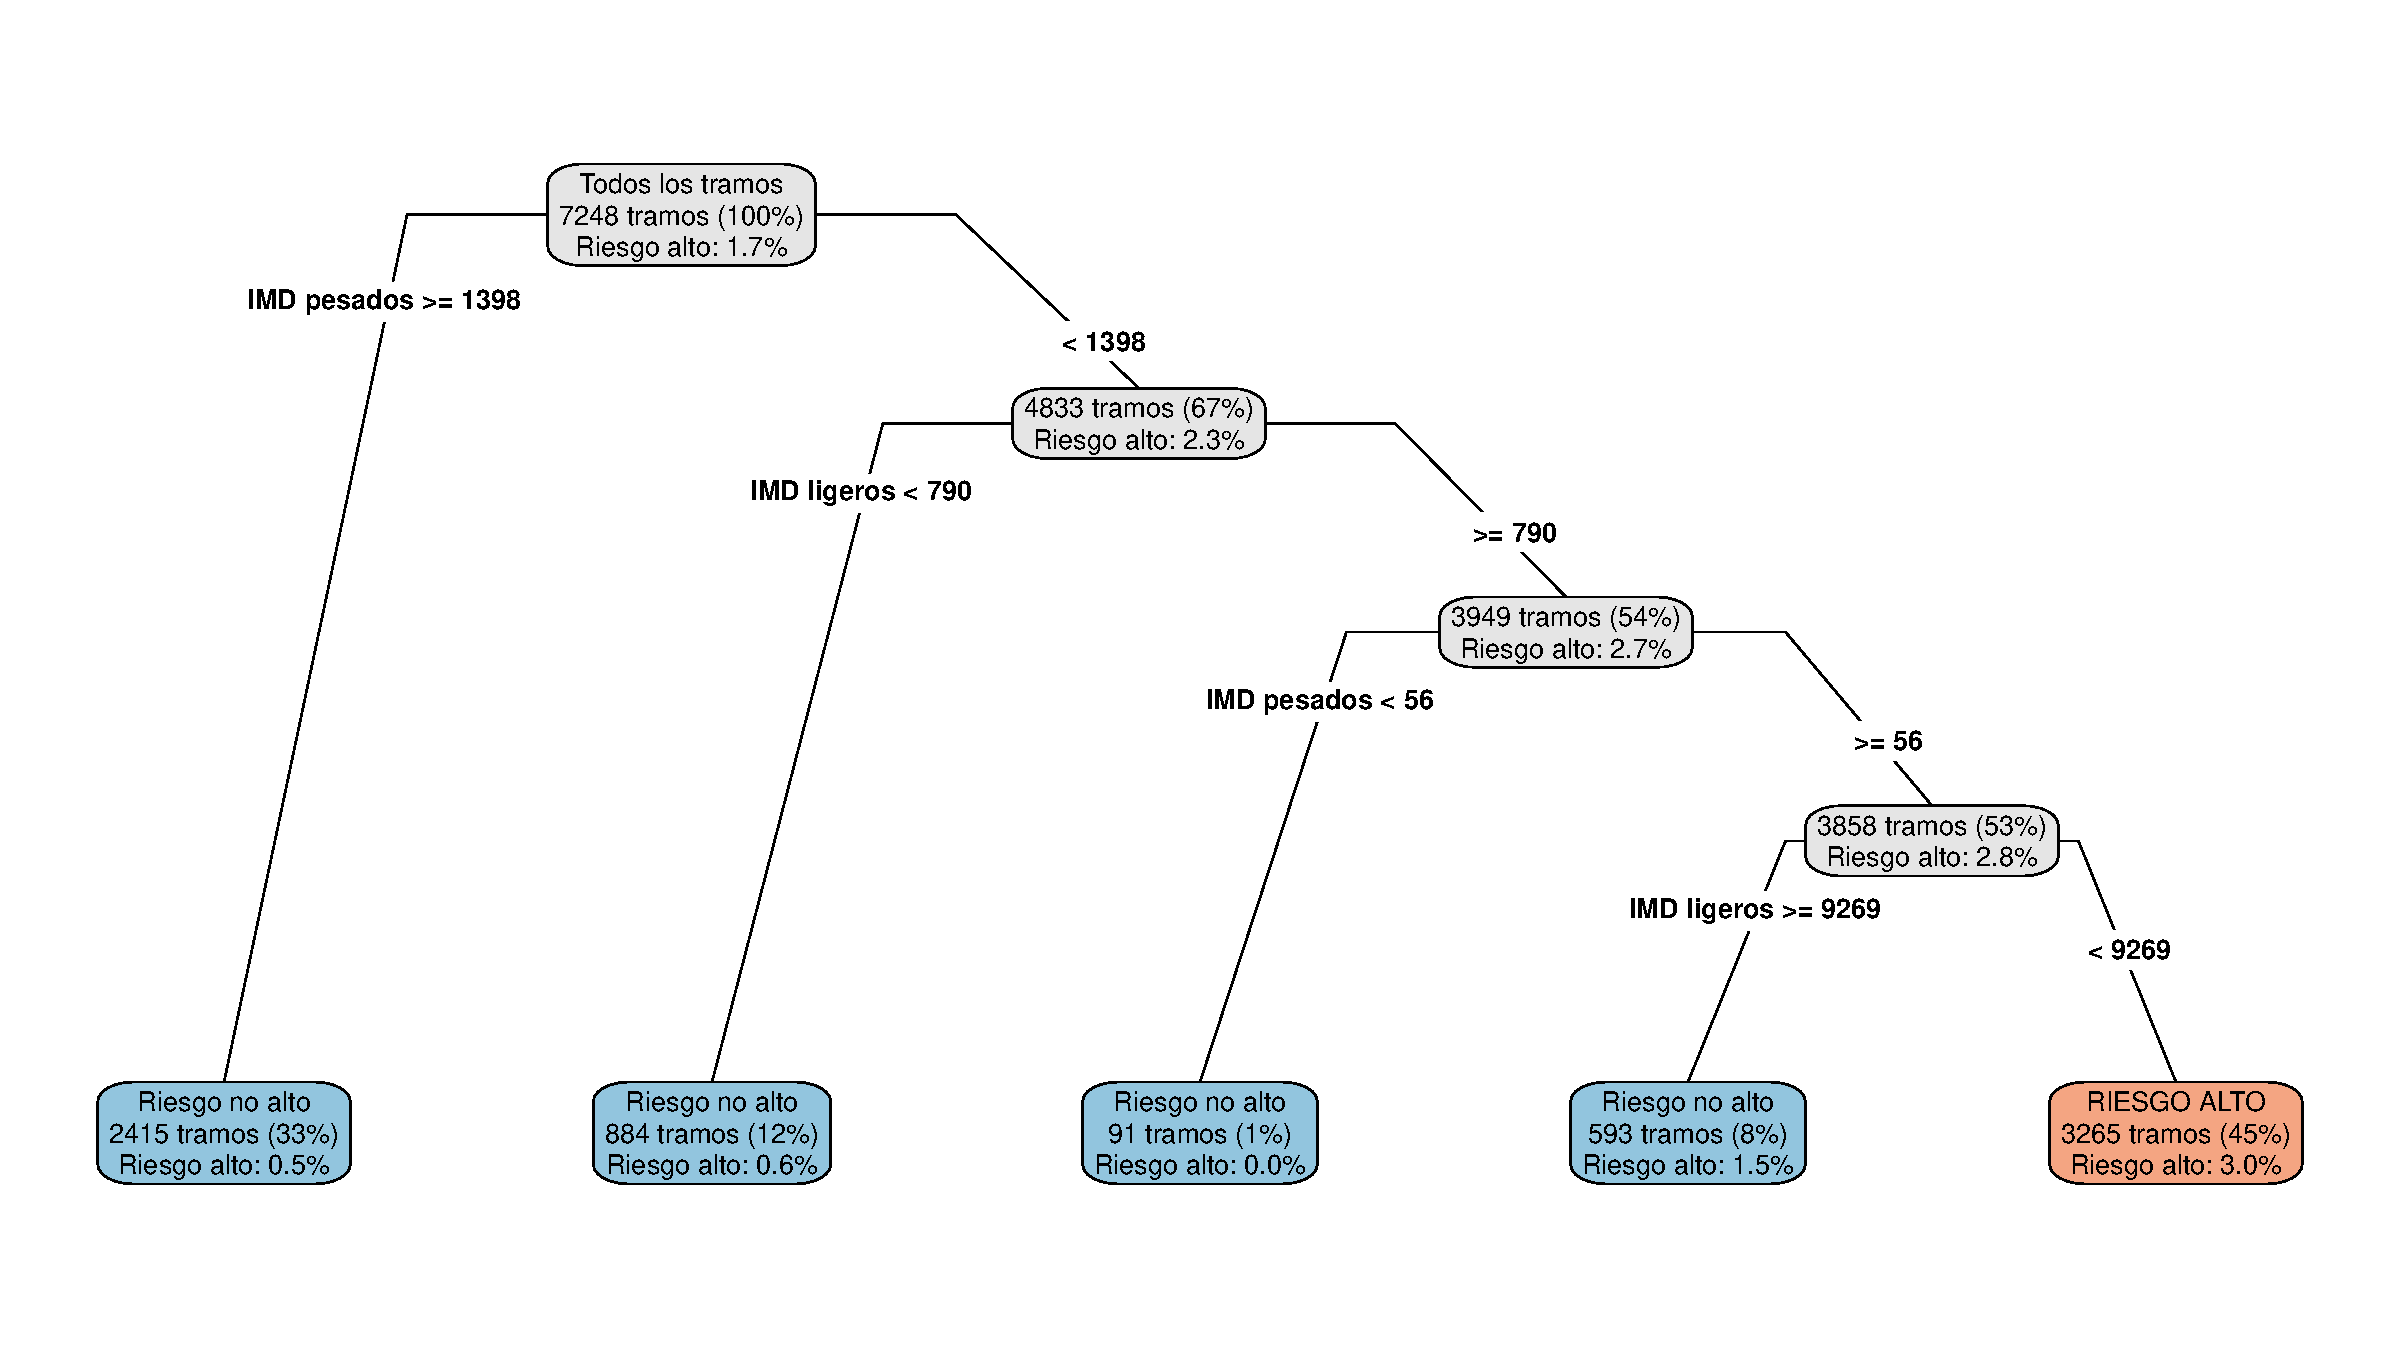
\includegraphics[width=\textwidth]{arboles6.3/arboltrim24.pdf}
    \caption{Árbol de clasificación definitivo para la base de Tramos IM 2024.}
    \label{fig:arbol_tramos_im_2024}
\end{sidewaysfigure}
\clearpage

El árbol tiene cinco hojas y, a diferencia de los anteriores, no utiliza el tipo de vía, sino únicamente las intensidades de tráfico:
 
\begin{itemize}
    \item Los tramos con 1398 o más vehículos pesados diarios (2415 tramos, el $33\%$) se clasifican como riesgo no alto, con un $0.5\%$ de tramos de riesgo alto.
    \item Entre los tramos con menos de 1398 pesados (4833 tramos, el $67\%$), los que tienen menos de 790 vehículos ligeros diarios (884 tramos, el $12\%$) se clasifican como riesgo no alto ($0.6\%$).
    \item Los tramos con menos de 1398 pesados y 790 o más ligeros (3949 tramos, el $54\%$) se dividen de nuevo. Se clasifican como riesgo no alto los que tienen menos de 56 pesados diarios (91 tramos, ninguno de riesgo alto) y los que tienen 9269 o más ligeros (593 tramos, $1.5\%$), mientras que el resto (3265 tramos, el $45\%$) se clasifica como riesgo alto, con una proporción real del $3.0\%$.
\end{itemize}
 
El riesgo alto de mortalidad se concentra así en los tramos con una intensidad de pesados moderada y una intensidad de ligeros intermedia, ni muy baja ni muy alta. La hoja de menos de 56 pesados contiene muy pocos tramos, por lo que no debe interpretarse como un patrón general.
 
\subsection{Base de Datos de Accidentes IP 2023}
 
El árbol construido con el conjunto de entrenamiento balanceado y la combinación elegida (cp $=0.005$ y minbucket $=80$) obtiene en el conjunto de prueba un AUC de $0.793$, con un intervalo de confianza al $95\%$ de $(0.776,\ 0.809)$. Este valor es muy similar al estimado mediante validación cruzada ($0.801$), lo que indica que el árbol no está sobreajustado. La Tabla~\ref{tab:confusion_acc_ip_2023} recoge la matriz de confusión sobre el conjunto de prueba.
 
\begin{table}[H]
    \centering
    \vspace{0.3cm}
    \renewcommand{\arraystretch}{1.3}
    \begin{tabular}{lcc}
        \toprule
        & \multicolumn{2}{c}{\textbf{Real}} \\
        \cmidrule(lr){2-3}
        \textbf{Predicción} & \textbf{No} & \textbf{Sí} \\
        \midrule
        No & 1447 & 218 \\
        Sí & 277  & 639 \\
        \bottomrule
    \end{tabular}
    \caption{Matriz de confusión del árbol en el conjunto de prueba (Accidentes IP 2023).}
    \label{tab:confusion_acc_ip_2023}
\end{table}
 
\vspace{0.5cm}
 
A partir de ella se obtiene una sensibilidad de $0.746$, una especificidad de $0.839$, una precisión de $0.698$ y una exactitud de $0.808$. A diferencia de las bases de Tramos, el árbol identifica la mayoría de los puntos de riesgo alto (639 de 857) sin clasificar como tales a una gran parte de los que no lo son. Como las clases están aquí menos desbalanceadas, la exactitud resulta más informativa y supera claramente el $66.8\%$ que obtendría un clasificador que asignara siempre la clase mayoritaria. La precisión es más del doble de la proporción de puntos de riesgo alto en el conjunto de prueba ($33.2\%$).
 
\vspace{0.5cm}
 
Estos valores son claramente superiores a los de las bases de Tramos, pero no son directamente comparables con ellos. Las bases de Accidentes solo contienen puntos kilométricos con al menos un siniestro, el índice de cada tramo se repite en todos sus puntos y, por la forma en que se definió la variable objetivo, aproximadamente un tercio de los registros son de riesgo alto. La partición por tramos descarta, en cambio, que la mejora se deba a que un mismo tramo aparezca a la vez en el conjunto de entrenamiento y en el de prueba.
 
\vspace{0.5cm}
 
La Figura~\ref{fig:arbol_accidentes_ip_2023} muestra el árbol definitivo, construido con la base de datos completa balanceada. En este caso, cada nodo indica el número de puntos kilométricos que contiene.

\clearpage

\begin{sidewaysfigure}
    \centering
    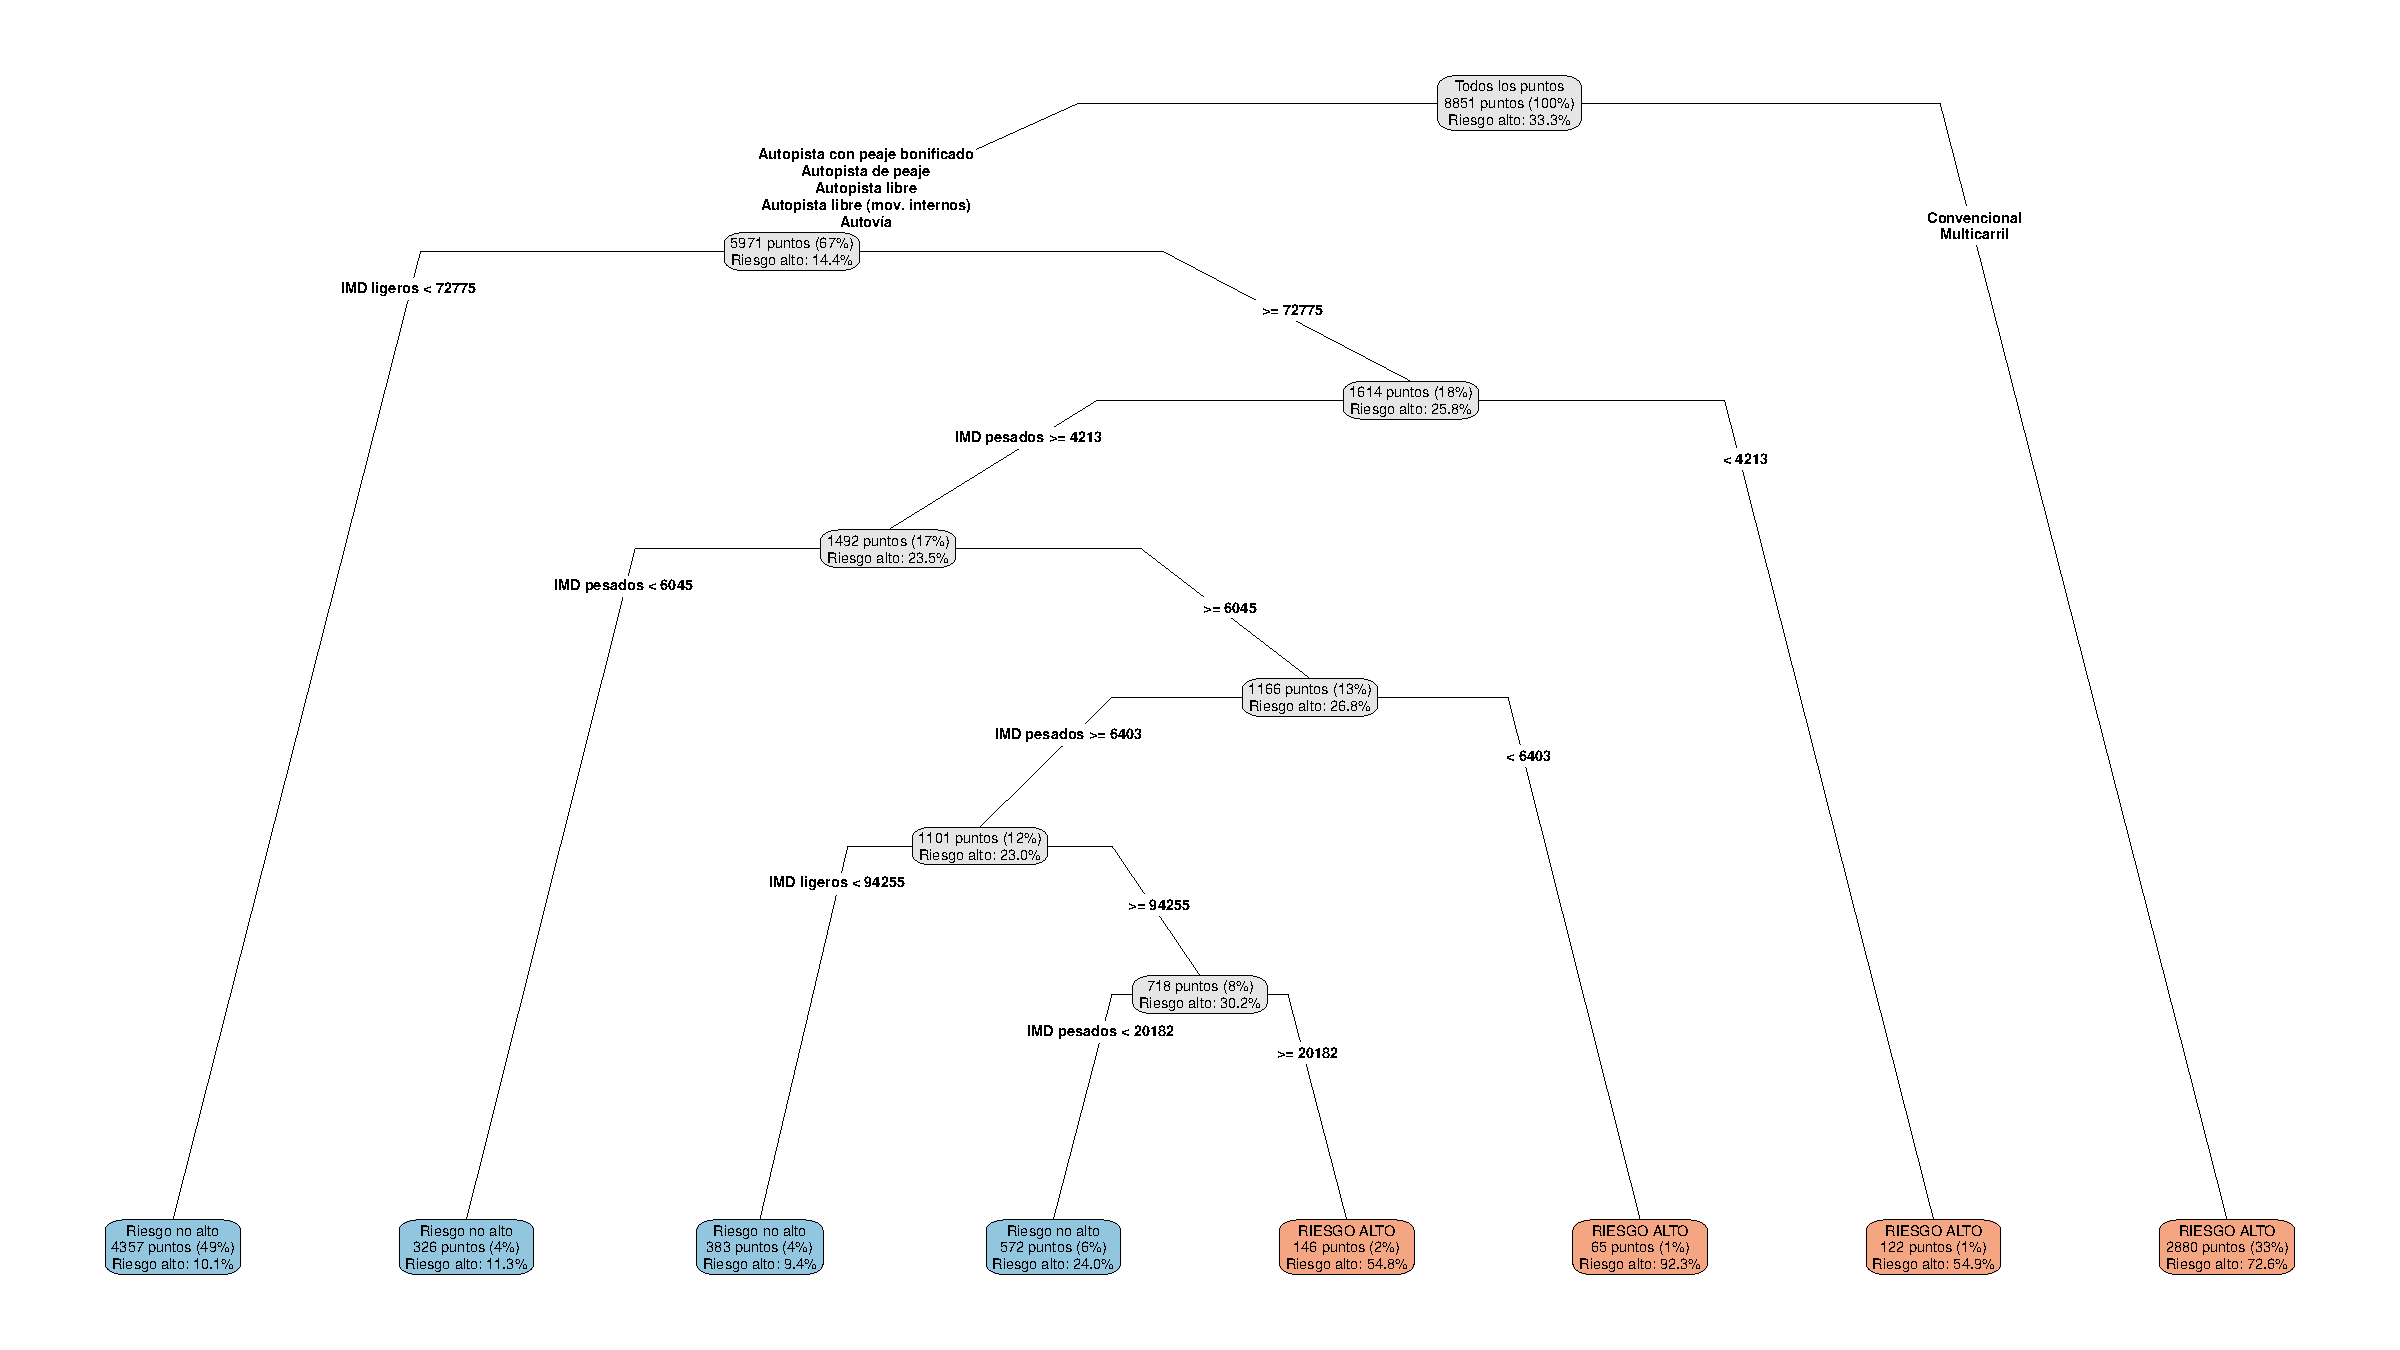
\includegraphics[width=\textwidth]{arboles6.3/arbolacip23.pdf}
    \caption{Árbol de clasificación definitivo para la base de Accidentes IP 2023.}
    \label{fig:arbol_accidentes_ip_2023}
\end{sidewaysfigure}
\clearpage

El árbol tiene ocho hojas, frente a las dos del árbol construido con el conjunto de entrenamiento, ya que al disponer de más registros se conservan más divisiones con los mismos parámetros. Su primera división se basa en el tipo de vía:
 
\begin{itemize}
    \item Los puntos situados en carreteras convencionales y multicarril (2880 puntos, el $33\%$) se clasifican como riesgo alto, con una proporción real del $72.6\%$.
    \item Los puntos situados en autopistas y autovías (5971 puntos, el $67\%$) presentan un $14.4\%$ de riesgo alto. Los que tienen menos de 72\,775 vehículos ligeros diarios (4357 puntos, el $49\%$) se clasifican como riesgo no alto ($10.1\%$).
    \item Los puntos de autopistas y autovías con 72\,775 o más vehículos ligeros diarios (1614 puntos, el $18\%$) se dividen en seis hojas según la intensidad de pesados y de ligeros. Tres de ellas se clasifican como riesgo alto: los puntos con menos de 4213 pesados diarios (122 puntos, $54.9\%$), los que tienen entre 6045 y 6403 pesados (65 puntos, $92.3\%$) y los que tienen 94\,255 o más ligeros y 20\,182 o más pesados (146 puntos, $54.8\%$). Las otras tres se clasifican como riesgo no alto, con proporciones de riesgo alto de entre el $9.4\%$ y el $24.0\%$.
\end{itemize}
 
La separación que consigue la primera división es muy marcada: la proporción de riesgo alto es cinco veces mayor en las carreteras convencionales y multicarril que en las vías de alta capacidad. Las divisiones dentro de las autopistas y autovías con más tráfico dan lugar a hojas pequeñas, algunas en intervalos muy estrechos de intensidad, como la de 65 puntos entre 6045 y 6403 pesados. Como los puntos kilométricos de un mismo tramo comparten el valor del índice, estas hojas pueden corresponder a muy pocos tramos, por lo que deben interpretarse con cautela.
 
\vspace{0.5cm}
 
Por último, al aplicar el árbol a los datos de 2024 se obtiene un AUC de $0.820$, superior incluso al obtenido en el conjunto de prueba de 2023.
 
\subsection{Base de Datos de Accidentes IM 2023}
 
El árbol construido con el conjunto de entrenamiento balanceado y la combinación elegida (cp $=0.05$ y minbucket $=120$) obtiene en el conjunto de prueba un AUC de $0.702$, con un intervalo de confianza al $95\%$ de $(0.663,\ 0.741)$. Este valor es notablemente inferior al estimado mediante validación cruzada ($0.758$), lo que indica que el árbol se ajusta en parte a particularidades del conjunto de entrenamiento. La Tabla~\ref{tab:confusion_acc_im_2023} recoge la matriz de confusión sobre el conjunto de prueba.
 
\begin{table}[H]
    \centering
    \vspace{0.3cm}
    \renewcommand{\arraystretch}{1.3}
    \begin{tabular}{lcc}
        \toprule
        & \multicolumn{2}{c}{\textbf{Real}} \\
        \cmidrule(lr){2-3}
        \textbf{Predicción} & \textbf{No} & \textbf{Sí} \\
        \midrule
        No & 1687 & 54 \\
        Sí & 666  & 97 \\
        \bottomrule
    \end{tabular}
    \caption{Matriz de confusión del árbol en el conjunto de prueba (Accidentes IM 2023).}
    \label{tab:confusion_acc_im_2023}
\end{table}
 
\vspace{0.5cm}
 
A partir de ella se obtiene una sensibilidad de $0.642$, una especificidad de $0.717$, una precisión de $0.127$ y una exactitud de $0.712$. El árbol detecta casi dos de cada tres puntos de riesgo alto (97 de 151), pero clasifica como tales a 666 puntos que no lo son. La precisión es baja en términos absolutos, aunque duplica la proporción de puntos de riesgo alto en el conjunto de prueba ($6.0\%$).
 
\vspace{0.5cm}
 
La Figura~\ref{fig:arbol_accidentes_im_2023} muestra el árbol definitivo, construido con la base de datos completa balanceada.

\clearpage

\begin{sidewaysfigure}
    \centering
    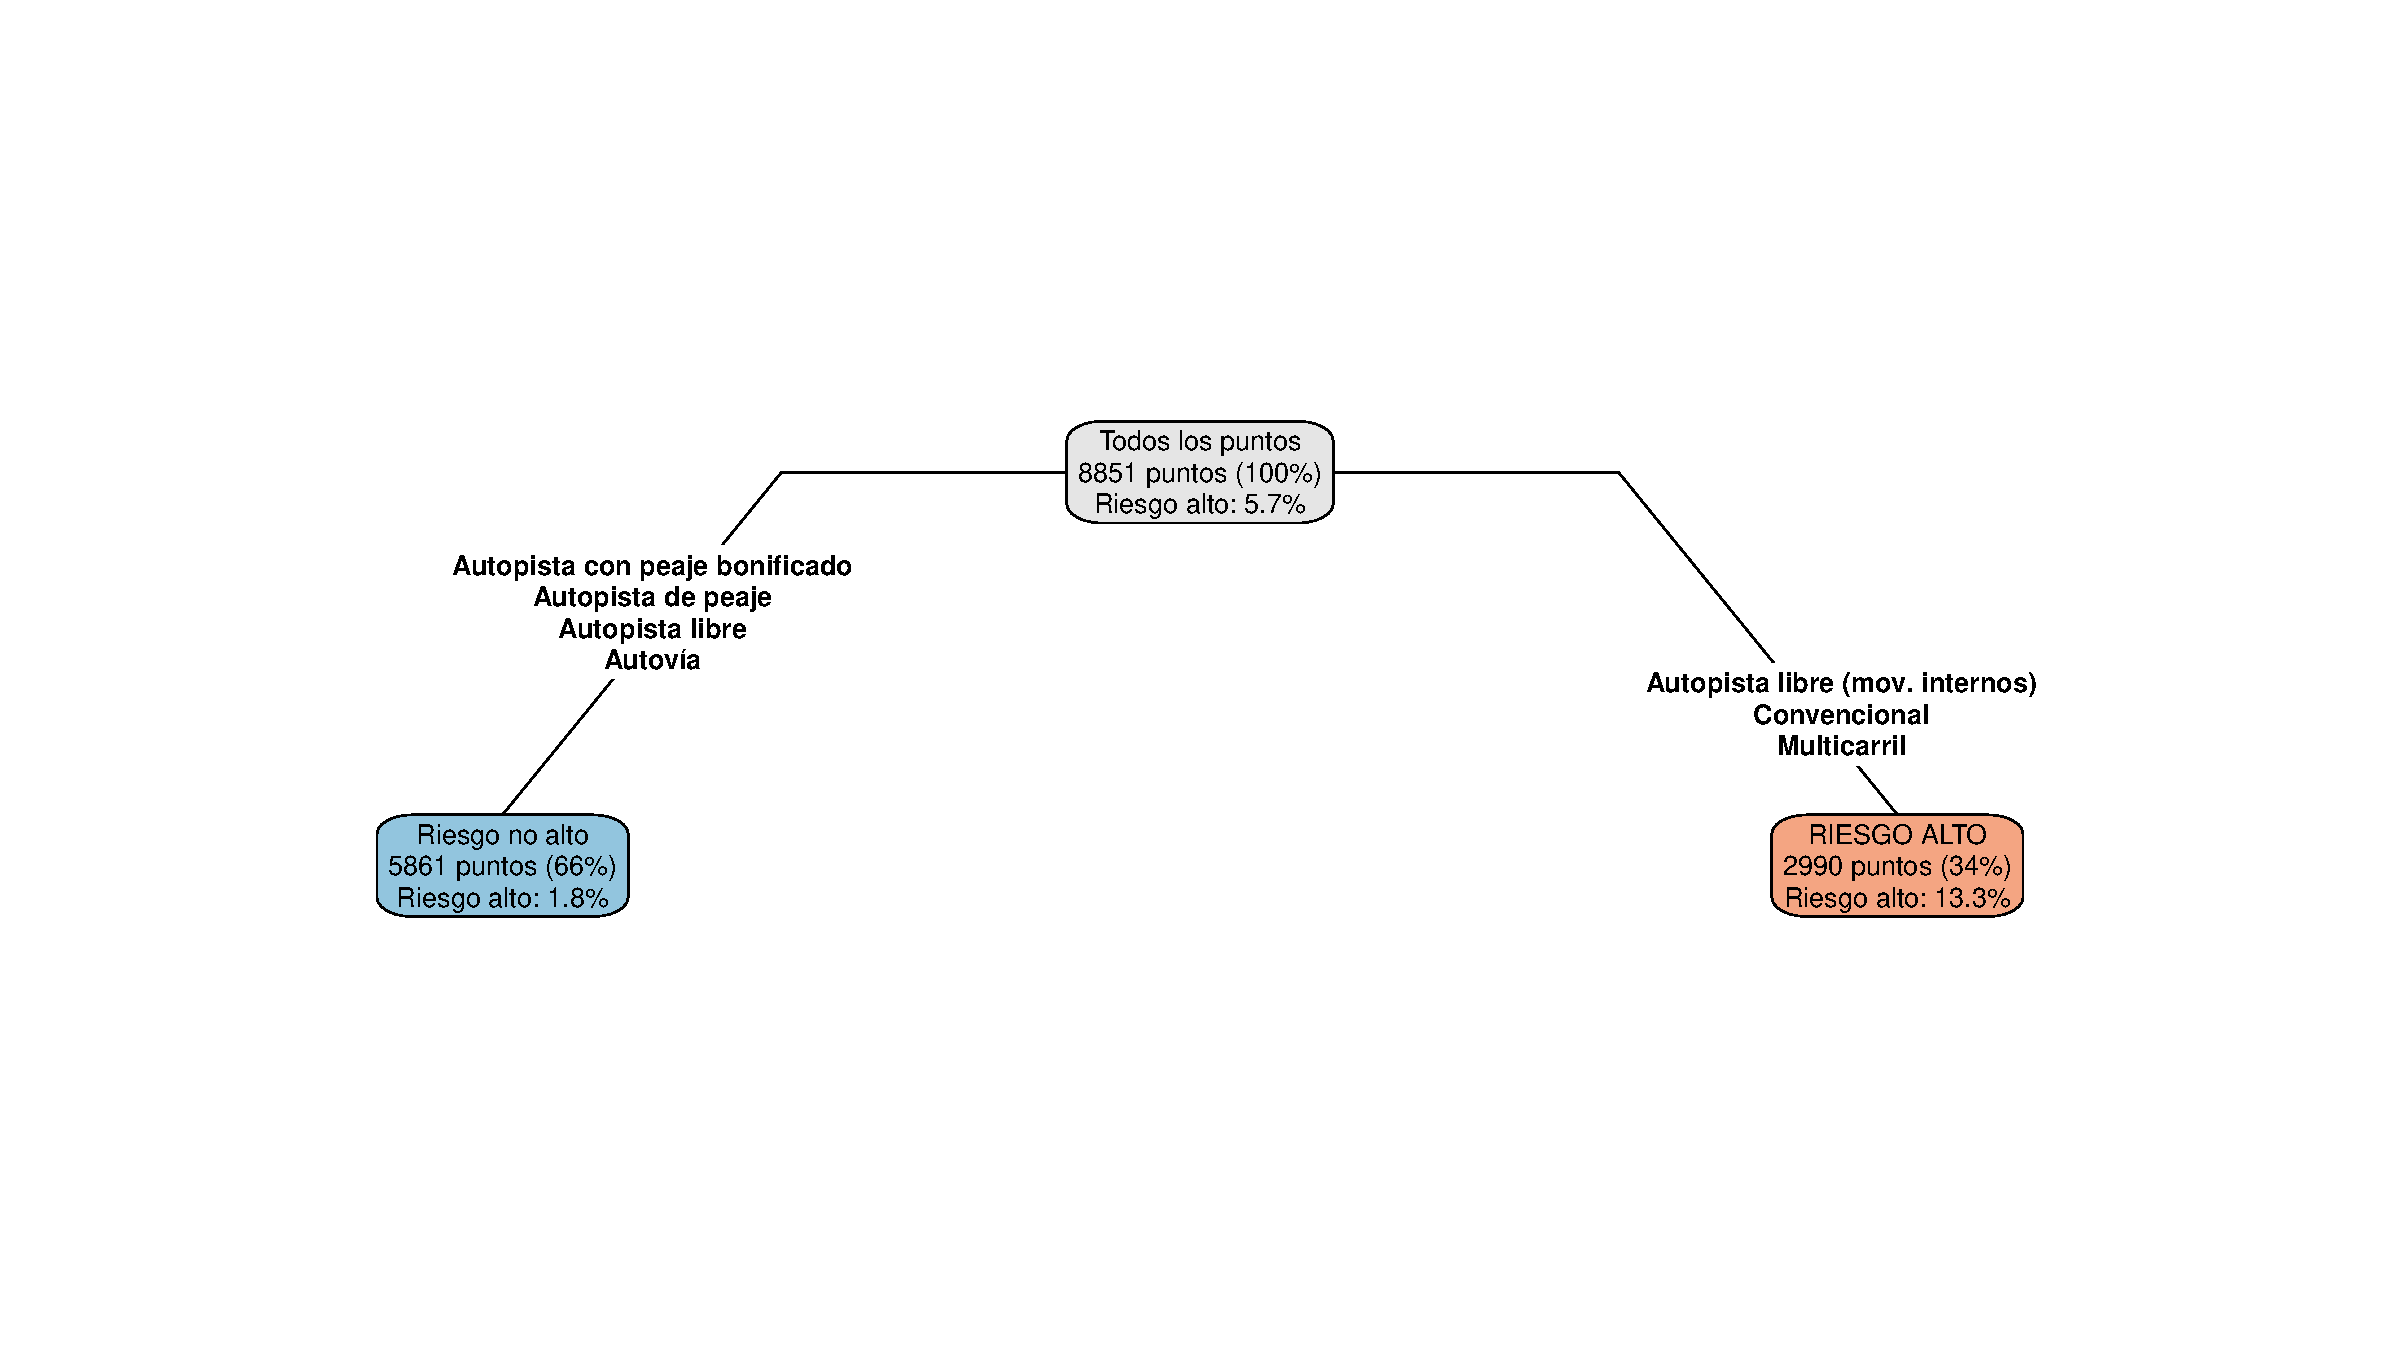
\includegraphics[width=\textwidth]{arboles6.3/arbolacim23.pdf}
    \caption{Árbol de clasificación definitivo para la base de Accidentes IM 2023.}
    \label{fig:arbol_accidentes_im_2023}
\end{sidewaysfigure}
\clearpage

El árbol tiene dos hojas y una única división por tipo de vía, frente a las tres hojas del árbol construido con el conjunto de entrenamiento: con la base completa balanceada, la segunda división no alcanza la mejora mínima que exige cp $=0.05$.
 
\begin{itemize}
    \item Los puntos situados en autopistas de peaje, con peaje bonificado y libres, y en autovías (5861 puntos, el $66\%$) se clasifican como riesgo no alto, con un $1.8\%$ de puntos de riesgo alto.
    \item Los puntos situados en carreteras convencionales, multicarril y autopistas libres para movimientos internos (2990 puntos, el $34\%$) se clasifican como riesgo alto, con una proporción real del $13.3\%$.
\end{itemize}
 
La proporción de riesgo alto es más de siete veces mayor en el segundo grupo, de modo que, como en el IP, el riesgo alto de mortalidad se concentra en las vías convencionales y multicarril.
 
\vspace{0.5cm}
 
Por último, al aplicar el árbol a los datos de 2024 se obtiene un AUC de $0.670$, algo inferior al obtenido en el conjunto de prueba de 2023.
 
\subsection{Base de Datos de Accidentes IP 2024}
 
El árbol construido con el conjunto de entrenamiento balanceado y la combinación elegida (cp $=0.005$ y minbucket $=120$) obtiene en el conjunto de prueba un AUC de $0.765$, con un intervalo de confianza al $95\%$ de $(0.748,\ 0.781)$, algo inferior al estimado mediante validación cruzada ($0.819$). La Tabla~\ref{tab:confusion_acc_ip_2024} recoge la matriz de confusión sobre el conjunto de prueba.
 
\begin{table}[H]
    \centering
    \vspace{0.3cm}
    \renewcommand{\arraystretch}{1.3}
    \begin{tabular}{lcc}
        \toprule
        & \multicolumn{2}{c}{\textbf{Real}} \\
        \cmidrule(lr){2-3}
        \textbf{Predicción} & \textbf{No} & \textbf{Sí} \\
        \midrule
        No & 1609 & 331 \\
        Sí & 246  & 647 \\
        \bottomrule
    \end{tabular}
    \caption{Matriz de confusión del árbol en el conjunto de prueba (Accidentes IP 2024).}
    \label{tab:confusion_acc_ip_2024}
\end{table}
 
\vspace{0.5cm}
 
A partir de ella se obtiene una sensibilidad de $0.662$, una especificidad de $0.867$, una precisión de $0.725$ y una exactitud de $0.796$. Respecto a 2023, el árbol detecta una proporción algo menor de los puntos de riesgo alto (647 de 978), pero comete menos falsos positivos. La exactitud supera el $65.5\%$ que obtendría un clasificador que asignara siempre la clase mayoritaria, y la precisión es más del doble de la proporción de puntos de riesgo alto en el conjunto de prueba ($34.5\%$).
 
\vspace{0.5cm}
 
La Figura~\ref{fig:arbol_accidentes_ip_2024} muestra el árbol definitivo, construido con la base de datos completa balanceada.

\clearpage

\begin{sidewaysfigure}
    \centering
    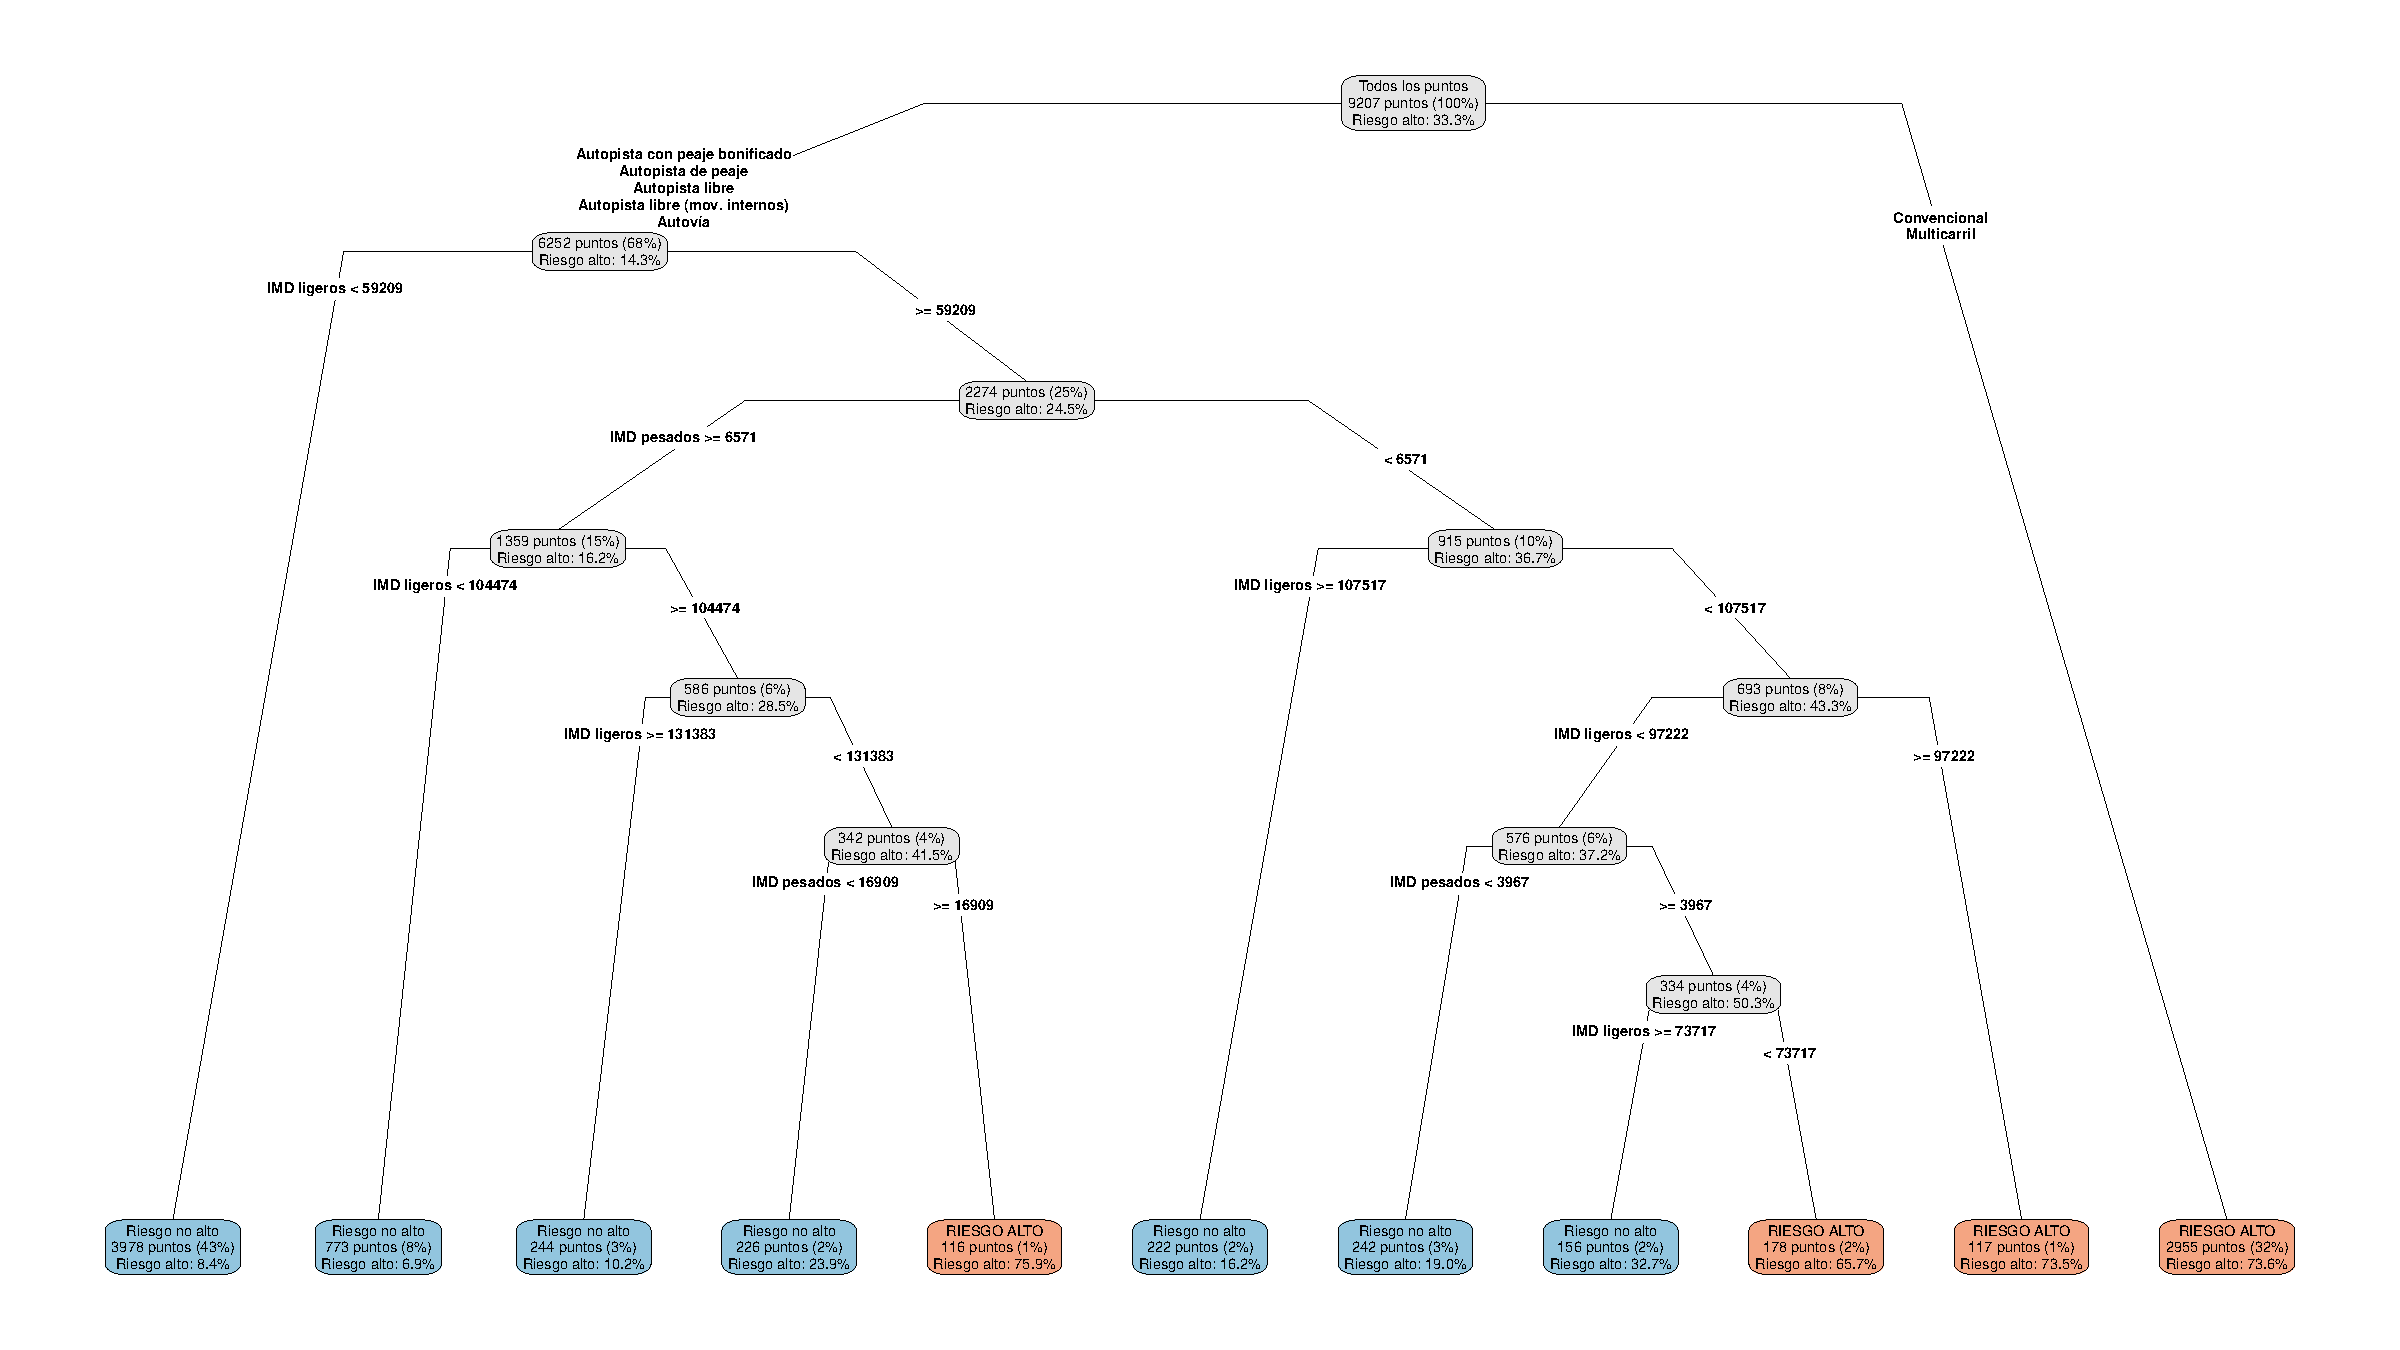
\includegraphics[width=\textwidth]{arboles6.3/arbolacip24.pdf}
    \caption{Árbol de clasificación definitivo para la base de Accidentes IP 2024.}
    \label{fig:arbol_accidentes_ip_2024}
\end{sidewaysfigure}
\clearpage


El árbol tiene once hojas, frente a las dos del árbol construido con el conjunto de entrenamiento. Su primera división es la misma que en 2023:
 
\begin{itemize}
    \item Los puntos situados en carreteras convencionales y multicarril (2955 puntos, el $32\%$) se clasifican como riesgo alto, con una proporción real del $73.6\%$.
    \item Los puntos situados en autopistas y autovías (6252 puntos, el $68\%$) presentan un $14.3\%$ de riesgo alto. Los que tienen menos de 59\,209 vehículos ligeros diarios (3978 puntos, el $43\%$) se clasifican como riesgo no alto ($8.4\%$).
    \item Los puntos de autopistas y autovías con 59\,209 o más vehículos ligeros diarios (2274 puntos, el $25\%$) se dividen en nueve hojas según la intensidad de ligeros y de pesados. Tres de ellas, con menos de 200 puntos cada una, se clasifican como riesgo alto: los puntos con entre 59\,209 y 73\,717 ligeros y entre 3967 y 6571 pesados (178 puntos, $65.7\%$), los que tienen entre 97\,222 y 107\,517 ligeros y menos de 6571 pesados (117 puntos, $73.5\%$), y los que tienen entre 104\,474 y 131\,383 ligeros y 16\,909 o más pesados (116 puntos, $75.9\%$). Las otras seis se clasifican como riesgo no alto, con proporciones de riesgo alto de entre el $6.9\%$ y el $32.7\%$.
\end{itemize}
 
Como en 2023, la estructura principal del árbol es la división por tipo de vía, con proporciones de riesgo alto prácticamente iguales en ambos años ($72.6\%$ y $73.6\%$ en las carreteras convencionales y multicarril). Las hojas adicionales dentro de las autopistas y autovías son pequeñas y corresponden a intervalos estrechos de intensidad de tráfico, por lo que, por la misma razón que en 2023, deben interpretarse con cautela.
 
\subsection{Base de Datos de Accidentes IM 2024}
 
El árbol construido con el conjunto de entrenamiento balanceado y la combinación elegida (cp $=0.05$ y minbucket $=20$) obtiene en el conjunto de prueba un AUC de $0.709$, con un intervalo de confianza al $95\%$ de $(0.676,\ 0.742)$, superior al estimado mediante validación cruzada ($0.668$). La Tabla~\ref{tab:confusion_acc_im_2024} recoge la matriz de confusión sobre el conjunto de prueba.
 
\begin{table}[H]
    \centering
    \vspace{0.3cm}
    \renewcommand{\arraystretch}{1.3}
    \begin{tabular}{lcc}
        \toprule
        & \multicolumn{2}{c}{\textbf{Real}} \\
        \cmidrule(lr){2-3}
        \textbf{Predicción} & \textbf{No} & \textbf{Sí} \\
        \midrule
        No & 1608 & 35  \\
        Sí & 928  & 127 \\
        \bottomrule
    \end{tabular}
    \caption{Matriz de confusión del árbol en el conjunto de prueba (Accidentes IM 2024).}
    \label{tab:confusion_acc_im_2024}
\end{table}
 
\vspace{0.5cm}
 
A partir de ella se obtiene una sensibilidad de $0.784$, una especificidad de $0.634$, una precisión de $0.120$ y una exactitud de $0.643$. El árbol detecta la mayoría de los puntos de riesgo alto (127 de 162), pero clasifica como tales a 928 puntos que no lo son. Como en 2023, la precisión es baja en términos absolutos, aunque duplica la proporción de puntos de riesgo alto en el conjunto de prueba ($6.0\%$).
 
\vspace{0.5cm}
 
La Figura~\ref{fig:arbol_accidentes_im_2024} muestra el árbol definitivo, construido con la base de datos completa balanceada.

\clearpage

\begin{sidewaysfigure}
    \centering
    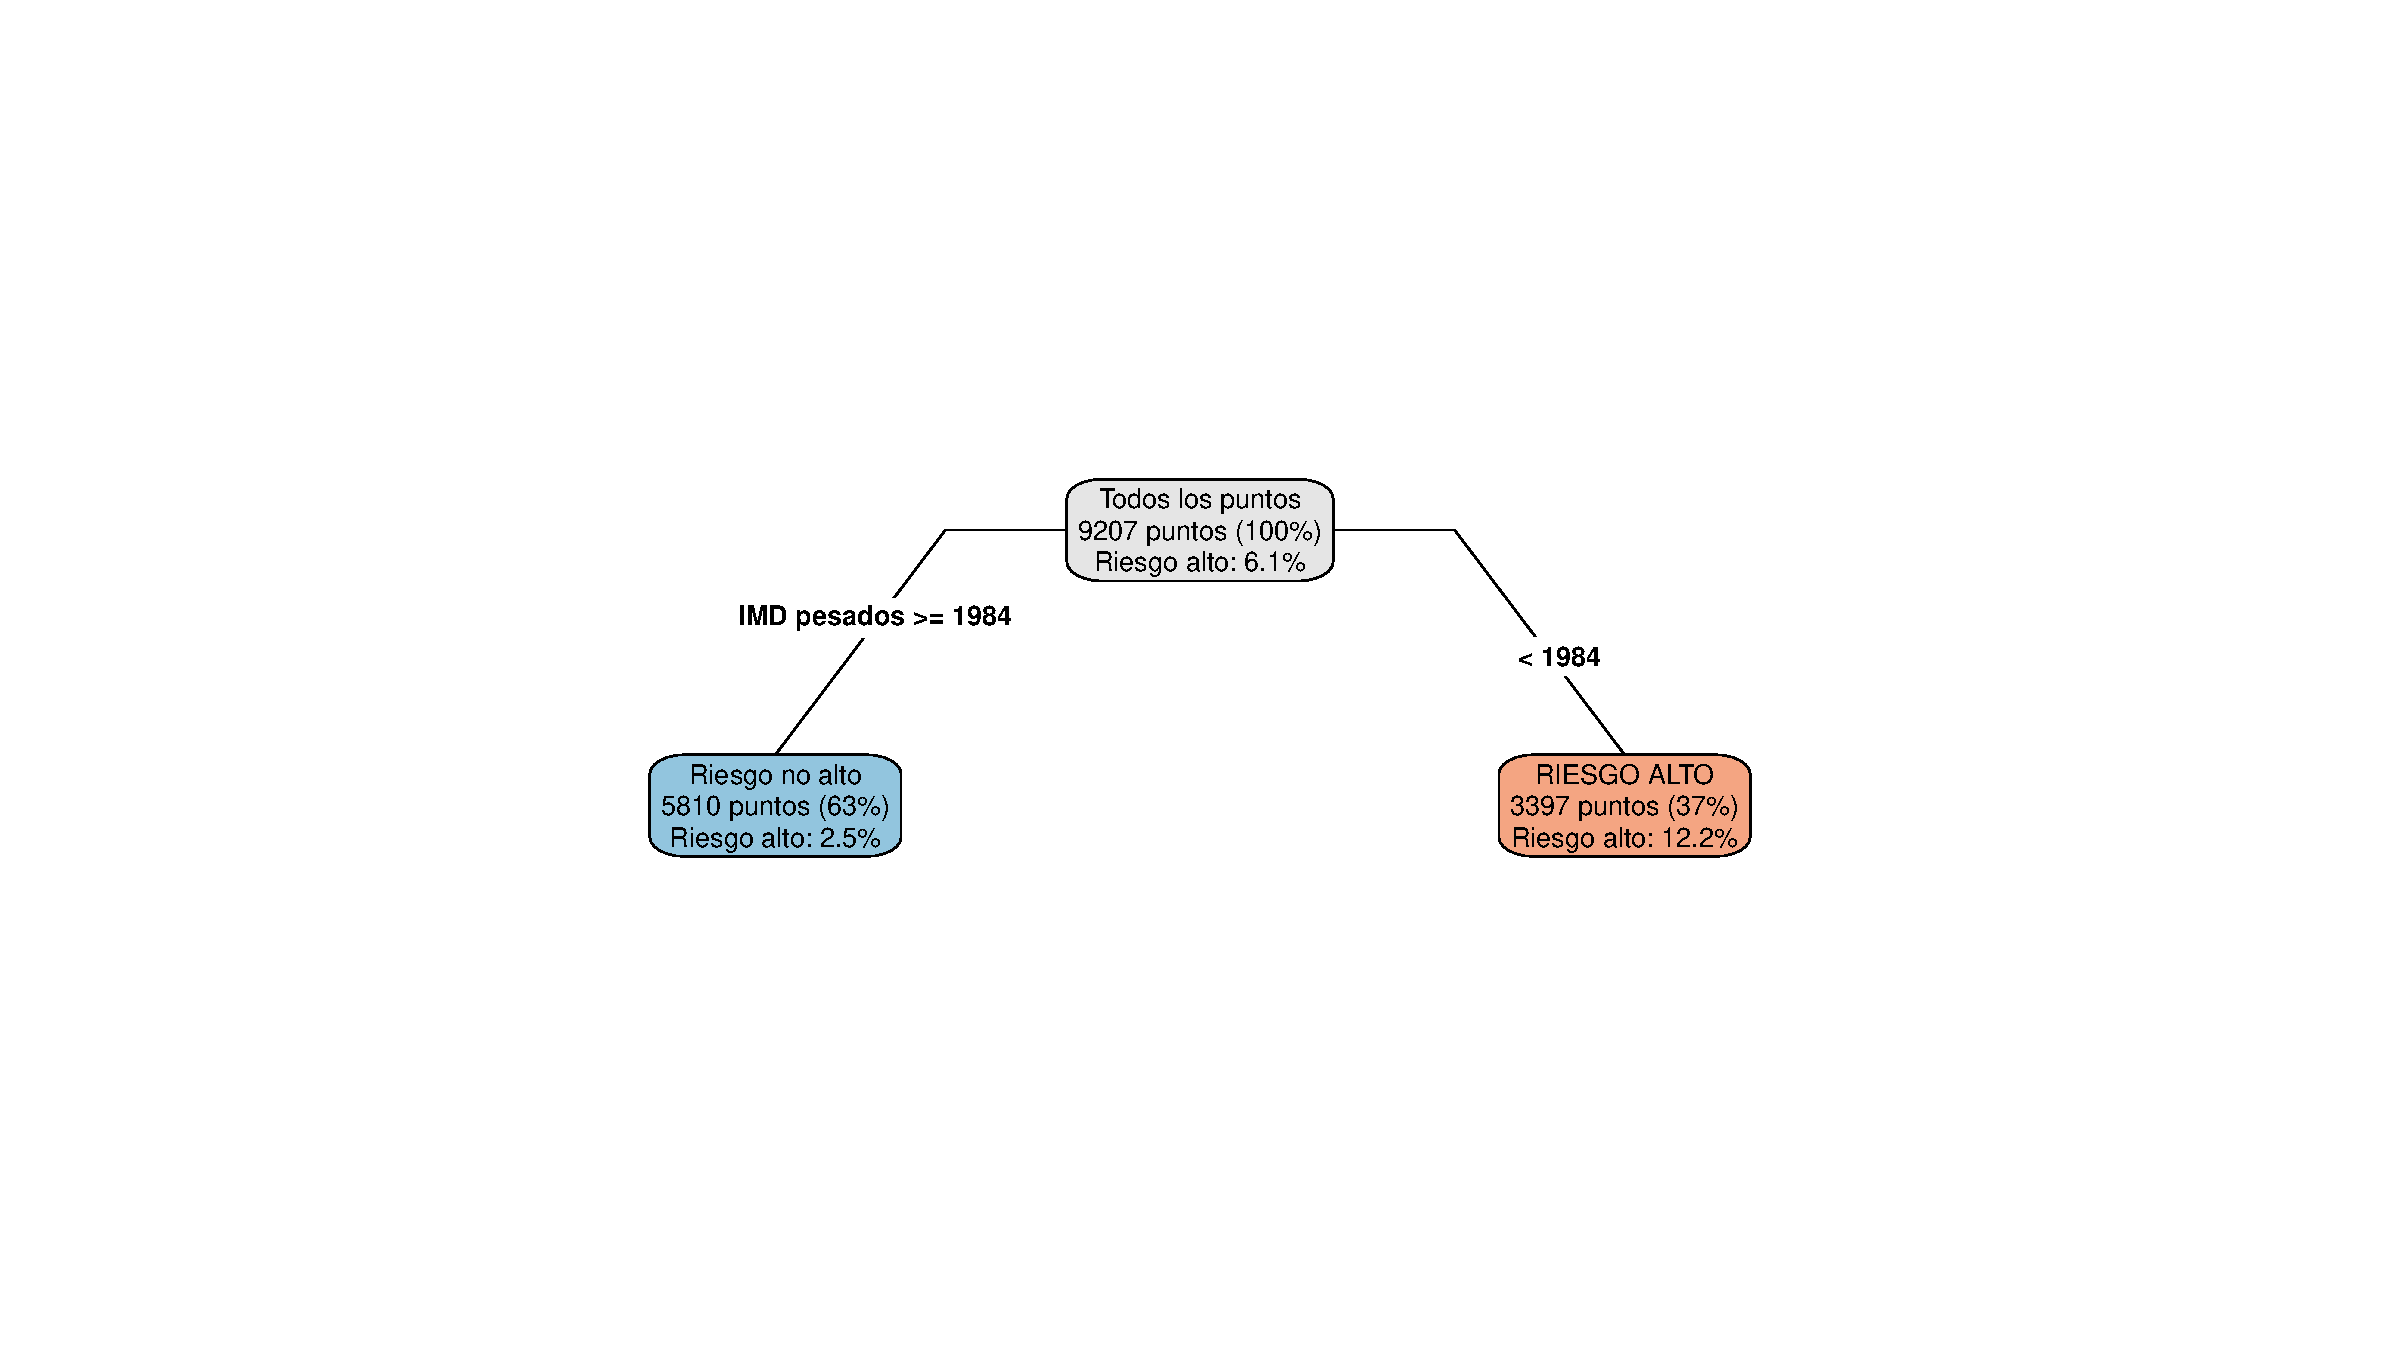
\includegraphics[width=\textwidth]{arboles6.3/arbolacim24.pdf}
    \caption{Árbol de clasificación definitivo para la base de Accidentes IM 2024.}
    \label{fig:arbol_accidentes_im_2024}
\end{sidewaysfigure}
\clearpage

El árbol tiene dos hojas y una única división, basada en la intensidad de vehículos pesados:
 
\begin{itemize}
    \item Los puntos con menos de 1984 pesados diarios (3397 puntos, el $37\%$) se clasifican como riesgo alto, con una proporción real del $12.2\%$.
    \item Los puntos con 1984 o más pesados diarios (5810 puntos, el $63\%$) se clasifican como riesgo no alto, con un $2.5\%$ de puntos de riesgo alto.
\end{itemize}
 
Los puntos con poco tráfico de pesados presentan, por tanto, una proporción de riesgo alto casi cinco veces mayor que el resto. A diferencia de 2023, la división no se basa en el tipo de vía, sino en la intensidad de vehículos pesados.
 
\subsection{Resumen de los árboles}
 
La Tabla~\ref{tab:resumen_arboles} reúne los resultados de los ocho árboles. La columna de validación temporal recoge el AUC obtenido al aplicar el árbol definitivo de 2023 a los datos de 2024, por lo que solo existe para las bases de 2023.
 
\begin{table}[H]
    \centering
    \small
    \setlength{\tabcolsep}{4pt}
    \renewcommand{\arraystretch}{1.3}
    \resizebox{\textwidth}{!}{%
    \begin{tabular}{llcccccccc}
        \toprule
        & & & \textbf{AUC} & \multicolumn{2}{c}{\textbf{AUC prueba}} & & & & \textbf{AUC} \\
        \cmidrule(lr){5-6}
        \textbf{Base} & \textbf{Índice} & \textbf{Hojas} & \textbf{VC} & \textbf{Valor} & \textbf{IC $95\%$} & \textbf{Sens.} & \textbf{Esp.} & \textbf{Prec.} & \textbf{temporal} \\
        \midrule
        Tramos 2023     & IP & 7  & 0.659 & 0.681 & (0.654, 0.709) & 0.391 & 0.811 & 0.261 & 0.673 \\
        Tramos 2023     & IM & 4  & 0.647 & 0.707 & (0.635, 0.780) & 0.528 & 0.765 & 0.036 & 0.637 \\
        Tramos 2024     & IP & 6  & 0.662 & 0.672 & (0.650, 0.693) & 0.862 & 0.475 & 0.225 & --    \\
        Tramos 2024     & IM & 5  & 0.621 & 0.598 & (0.513, 0.682) & 0.568 & 0.602 & 0.024 & --    \\
        \midrule
        Accidentes 2023 & IP & 8  & 0.801 & 0.793 & (0.776, 0.809) & 0.746 & 0.839 & 0.698 & 0.820 \\
        Accidentes 2023 & IM & 2  & 0.758 & 0.702 & (0.663, 0.741) & 0.642 & 0.717 & 0.127 & 0.670 \\
        Accidentes 2024 & IP & 11 & 0.819 & 0.765 & (0.748, 0.781) & 0.662 & 0.867 & 0.725 & --    \\
        Accidentes 2024 & IM & 2  & 0.668 & 0.709 & (0.676, 0.742) & 0.784 & 0.634 & 0.120 & --    \\
        \bottomrule
    \end{tabular}}
    \caption{Resumen de los árboles finales con balanceo en las ocho bases de datos. El número de hojas corresponde al árbol definitivo, construido con la base completa balanceada, y las medidas de prueba, al árbol construido con el conjunto de entrenamiento balanceado.}
    \label{tab:resumen_arboles}
\end{table}
 
\vspace{0.5cm}
 
En todas las bases el intervalo de confianza del AUC en el conjunto de prueba se sitúa por encima de $0.5$, de modo que los ocho árboles distinguen los registros de riesgo alto mejor que el azar, aunque en Tramos IM 2024 el margen es muy pequeño. Los árboles definitivos tienen entre dos y once hojas, pero su estructura principal es sencilla: el tipo de vía es la primera división en seis de los ocho, separando las autopistas y autovías, con un riesgo bajo, de las carreteras convencionales y, en general, multicarril. Las hojas adicionales de los árboles más grandes se apoyan en intervalos estrechos de intensidad de tráfico y en pocos registros. Los árboles del IP son, además, más estables que los del IM: su estructura se repite en los dos años y su AUC se mantiene en la validación temporal, mientras que en el IM tanto la estructura como el rendimiento cambian más de un año a otro. Las bases de Accidentes obtienen valores de AUC más altos que las de Tramos, aunque, como se ha indicado, estos valores no son directamente comparables por la distinta construcción de las bases.
 
%%%%%%%%%%%%%%%%%%FIN CAP 6 %%%%%%%%%%%%%%%%%%%%%%%%%%%%%%%%%%%%%%%%%%%%%%%

%%%%%%%%%%%%%%%%INICIO CAP 7 %%%%%%%%%%%%%%%%%%%%%%%%%%%%%%%%%%%%%%%%%%%%%%
\setcounter{chapter}{7}
\chapter*{Capítulo 7 \\ \vspace{1cm} Resultados}
\addcontentsline{toc}{chapter}{\protect\numberline{\thechapter}Resultados}

\setcounter{section}{0}
\setcounter{subsection}{0}
\setcounter{figure}{0}\setcounter{table}{0}

En este capítulo se interpretan los resultados obtenidos en los Capítulos~5 y~6. En primer lugar, se analizan los patrones identificados por las reglas de asociación y, a continuación, los de los árboles de clasificación. Por último, se analiza de forma conjunta el conocimiento extraído con ambas técnicas, comparando además los resultados de los dos años de estudio y de las bases de Tramos y de Accidentes.

\section{Interpretación de las reglas de asociación}

\subsection{Patrones de Siniestralidad}

Tras la ejecución del algoritmo \textit{Apriori} y el filtrado por la métrica \textit{Lift}, se aislaron las reglas de asociación más fuertes. La interpretación de estos resultados nos permite extraer tres conclusiones analíticas fundamentales sobre el comportamiento del riesgo en la red viaria.

\subsubsection{Comparación de las reglas según el tipo de base de datos}
Las reglas obtenidas en las bases de Accidentes presentan valores de confianza y \textit{Lift} claramente superiores a los de las bases de Tramos. Por ejemplo, en Tramos la regla con mayor confianza alcanza $0.224$, mientras que en Accidentes varias reglas superan el $0.59$ e incluso alcanzan el $100\%$.

\vspace{0.5cm}

Esta diferencia se debe, en primer lugar, a que la confianza que puede alcanzar una regla depende de la frecuencia de su consecuente: las categorías \textit{Alto} y \textit{Muy Alto} del IP suponen aproximadamente el 15\% de los tramos las dos juntas y las del IM menos del 2\%, frente a un 33\% de los puntos kilométricos en las bases de Accidentes con el IP. En segundo lugar, la base de datos de Accidentes solo contiene puntos kilométricos con al menos un siniestro, y el índice de cada tramo se repite en todos sus puntos, de modo que los tramos con más accidentes pesan más y los tramos sin siniestros no aparecen. Por tanto, los valores más altos de confianza y \textit{Lift} de las reglas de accidentes no indican por sí mismos un mayor riesgo, sino una construcción distinta de la base de datos. Lo que sí aporta esta base es un mayor número de registros por regla: algunas reglas se apoyan en más de 600 puntos kilométricos, aunque estos no son independientes entre sí.

\subsubsection{La Paradoja de la Vía Despejada}
Una de las conclusiones más llamativas extraídas por el algoritmo contradice en parte el mito habitual de que los accidentes más graves ocurren siempre donde hay mucha congestión o un elevado tráfico de camiones. Las reglas muestran que las categorías de mayor riesgo no se concentran únicamente en las vías más transitadas, y que las vías con tráfico muy bajo aparecen de forma recurrente en los patrones de peligrosidad y mortalidad. Sin embargo, este patrón no es tan sistemático como cabría pensar: en la base de Tramos, las reglas con mayor \textit{Lift} corresponden a niveles de tráfico medios y altos.

\begin{itemize}
    \item \textbf{Carreteras Convencionales:} Son el tipo de vía presente en la mayoría de las reglas. En la base de Tramos, las más fuertes asocian la carretera convencional con intensidades de tráfico medias o altas a un IP \textit{Alto} (Tabla~\ref{tab:reglas_tramos}), y las de tráfico muy bajo aparecen con un \textit{Lift} menor (130 tramos y \textit{Lift} $1.85$ en 2023). En la base de Accidentes, la combinación de una carretera convencional con un tráfico ligero y pesado muy bajo se asocia a un IP \textit{Muy Alto} (confianza $0.591$ y $0.606$, con 612 y 649 registros) y a un IM \textit{Muy Alto} (\textit{Lift} $4.19$ y $3.72$, con 124 y 122 registros), es decir, a una probabilidad de pertenecer a esa categoría de mortalidad entre 3.7 y 4.2 veces mayor que en el conjunto de la base.
    
    \item \textbf{Vías Multicarril:} En 2023 este mismo patrón aparece también en vías de alta capacidad, aunque con menos registros: en la base de Accidentes, las vías multicarril con tráfico ligero o pesado muy bajo se asocian a un IP \textit{Muy Alto} (28 y 39 registros, con confianzas de 0.933 y 0.672). En 2024 este patrón se mantiene, aunque con menor Lift (la regla \textit{Multicarril + Pesados (Muy Bajo)} $\Rightarrow$ \textit{IP (Muy Alto)} se apoya en 31 registros, con una confianza de $0.596$ y un Lift de $3.58$), y las reglas de las vías multicarril con mayor Lift corresponden a un tráfico ligero medio-alto o alto (Tabla~\ref{tab:reglas_accidentes}).
    
    \item \textbf{Autopistas libres con tráfico elevado:} También existen reglas en sentido contrario. En la base de Accidentes, la combinación de \textit{Autopista libre}, tráfico ligero \textit{Muy Alto} y tráfico pesado \textit{Medio} implica un IP \textit{Alto} en el $100\%$ de los casos de ambos años (23 y 30 registros), por lo que el riesgo no es exclusivo de las vías con poco tráfico.
\end{itemize}

\vspace{0.5cm}

Los datos disponibles no permiten determinar la causa de estos patrones, aunque pueden plantearse dos posibles explicaciones. 

\vspace{0.5cm}

La primera tiene que ver con el comportamiento del conductor: cuando circula por una vía vacía, su percepción del riesgo podría disminuir y generarse un falso sentido de seguridad que incite a aumentar la velocidad, de modo que cualquier error, distracción o salida de vía terminaría causando un accidente más severo. Sin embargo, los datos disponibles no incluyen la velocidad ni el comportamiento de los conductores, por lo que esta explicación es una hipótesis y no se deduce de los resultados. 

\vspace{0.5cm}

La segunda es de carácter estadístico: el IP se calcula dividiendo entre la exposición (intensidad de tráfico y longitud del tramo), por lo que en los tramos con poco tráfico un único accidente puede elevar mucho su valor, lo que facilitaría que alcancen las categorías más altas. Para descartarlo sería necesario comprobar que el patrón se mantiene con más años de datos.

\subsubsection{Consistencia entre Años y Alcance de los Resultados}

Al comparar los dos años se observa que parte de los patrones se repiten. Esta comparación sirve como validación de las reglas frente al riesgo de reglas espurias descrito en el apartado 4.1.5: una regla que se obtiene de forma independiente en los dos años es más fiable que una que aparece en uno solo. 

\vspace{0.5cm}

En la base de Tramos, las carreteras convencionales con tráfico ligero y pesado medio-alto o alto se asocian a un IP \textit{Alto} tanto en 2023 como en 2024. En la base de Accidentes también coinciden los dos años en las reglas de \textit{Autopista libre} y en la de carretera convencional con tráfico muy bajo, que se asocia tanto al IP como al IM \textit{Muy Alto}. 

\vspace{0.5cm}

En cambio, las reglas del IM en la base de Tramos apenas se repiten entre años: solo \textit{Pesados (Medio Alto)} $\Rightarrow$ \textit{IM (Alto)} aparece en ambos, mientras que en el resto en 2023 predominan las intensidades medias y medio-altas y en 2024 aparece además el tráfico ligero bajo, con confianzas de en torno al $2\%$ y apoyadas en entre 15 y 27 tramos. Esto se explica porque solo una pequeña parte de los tramos (361 en 2023 y 369 en 2024, alrededor del $5\%$) registra algún fallecido, por lo que sus resultados no son concluyentes.

\vspace{0.5cm}

En conjunto, las asociaciones encontradas son de intensidad moderada: en la base de Tramos el \textit{Lift} se sitúa entre 2 y 3 y las confianzas son bajas, lo que indica que el tipo de vía y la intensidad de tráfico explican solo una parte del riesgo. Factores no incluidos en los datos, como el trazado de la vía, la velocidad, las condiciones meteorológicas o el horario, quedan como posibles líneas de trabajo futuro. Por ello, los resultados deben entenderse como una identificación de contextos en los que la siniestralidad relativa es mayor, y no como una explicación de sus causas.

\section{Interpretación de los árboles de clasificación}
 
Los ocho árboles construidos en el Capítulo~6 permiten extraer tres conclusiones principales sobre la relación entre el contexto de la vía y el riesgo: el tipo de vía es el factor que más separa los registros de riesgo alto, la intensidad de tráfico matiza este riesgo de forma distinta en la peligrosidad y en la mortalidad, y la capacidad de estas variables para predecir el riesgo es limitada.
 
\subsection{El tipo de vía como factor principal}
 
El tipo de vía es la primera división en seis de los ocho árboles, y en todos ellos separa las autopistas y autovías, con un riesgo bajo, de las carreteras convencionales, a las que se asigna un riesgo mayor. En el IP de Tramos, solo el $4.5\%$ de los tramos de autopistas y autovías es de riesgo alto en 2023, y el $4.7\%$ en 2024, frente al $14.5\%$ y el $15.0\%$ del conjunto de los tramos. En el IP de Accidentes la diferencia es aún más marcada: el $72.6\%$ de los puntos kilométricos con siniestros de las carreteras convencionales y multicarril es de riesgo alto en 2023, y el $73.6\%$ en 2024, frente a algo más del $14\%$ en las autopistas y autovías.
 
\vspace{0.5cm}
 
Las carreteras multicarril no presentan un comportamiento homogéneo. En el IP y en el IM de Accidentes de 2023 se agrupan con las carreteras convencionales, mientras que en el IM de Tramos de 2023 se agrupan con las vías de alta capacidad, que presentan solo un $0.4\%$ de tramos de riesgo alto.
 
\vspace{0.5cm}
 
Este resultado es coherente con las características de la infraestructura. Las autopistas y autovías tienen calzadas separadas, accesos controlados y ausencia de cruces al mismo nivel, mientras que en las carreteras convencionales los adelantamientos, las intersecciones y la circulación en ambos sentidos por la misma calzada aumentan las posibilidades de accidente \cite{ingenieriacarreteras}. No obstante, los datos disponibles no incluyen estas características, por lo que esta explicación no se deduce directamente de los resultados.
 
\subsection{El papel de la intensidad de tráfico}
 
Dentro de cada tipo de vía, los árboles utilizan la intensidad de tráfico para matizar el riesgo, con un comportamiento distinto en el IP y en el IM.
 
\vspace{0.5cm}
 
\textbf{Peligrosidad (IP).} En las bases de Tramos, dentro de las carreteras convencionales y multicarril el riesgo aumenta con la intensidad de tráfico ligero. Los tramos con muy poco tráfico (menos de 265 vehículos ligeros diarios en 2023 y de 385 en 2024) presentan una proporción de riesgo alto del $6.5\%$ y del $7.4\%$, inferior a la de la base, mientras que los de más de 3751 y 4784 vehículos ligeros alcanzan el $25.7\%$ y el $25.2\%$, respectivamente. La estructura se repite en los dos años con puntos de corte del mismo orden, lo que indica que el patrón es estable.
 
\vspace{0.5cm}
 
\textbf{Mortalidad (IM).} En el IM, el riesgo alto se concentra en los tramos con un tráfico intermedio, y no en los extremos. En Tramos 2023, la hoja de riesgo alto reúne las carreteras convencionales con 129 o más vehículos pesados y menos de 8688 ligeros diarios ($3.2\%$ de riesgo alto). En Tramos 2024, el árbol prescinde del tipo de vía y la hoja de riesgo alto recoge los tramos con entre 56 y 1398 pesados y entre 790 y 9269 ligeros ($3.0\%$). En ambos años, los tramos con tráfico muy bajo o con mucho tráfico de pesados presentan una proporción de riesgo alto muy inferior (por ejemplo, del $0.5\%$ en los tramos con 1398 o más pesados en 2024). En las bases de Accidentes, el árbol del IM de 2024 separa los puntos con menos de 1984 pesados diarios, con un $12.2\%$ de riesgo alto, de los demás, con un $2.5\%$, de modo que entre los puntos con siniestros la mortalidad es mayor donde circulan menos vehículos pesados.
 
\vspace{0.5cm}
 
Los árboles más grandes, de seis a once hojas, añaden divisiones dentro de las autopistas y autovías con mucho tráfico, algunas en intervalos muy estrechos de intensidad (por ejemplo, entre 6045 y 6403 pesados diarios en Accidentes IP 2023). Como ya se indicó en el Capítulo~6, estas hojas reúnen pocos registros y, en las bases de Accidentes, pueden corresponder a muy pocos tramos, por lo que no deben interpretarse como patrones generales.
 
\subsection{Capacidad predictiva y estabilidad}
 
El AUC de los árboles en el conjunto de prueba se sitúa entre $0.60$ y $0.71$ en las bases de Tramos y entre $0.70$ y $0.79$ en las de Accidentes. Son valores moderados, que confirman que el tipo de vía y la intensidad de tráfico permiten distinguir parcialmente los registros de riesgo alto, pero que gran parte del riesgo depende de factores no incluidos en los datos.
 
\vspace{0.5cm}
 
Desde un punto de vista práctico, los árboles pueden utilizarse como una herramienta de priorización. En Tramos IP 2023, por ejemplo, el árbol señala como riesgo alto al $22\%$ de los tramos del conjunto de prueba, y entre ellos la proporción de tramos realmente de riesgo alto es del $26.1\%$, 1.8 veces la del conjunto ($14.5\%$). Revisar en primer lugar los tramos señalados por el árbol permite, por tanto, concentrar los recursos en un grupo con una proporción de riesgo alto claramente superior a la media, aunque una parte de los tramos de riesgo alto quede fuera de él.
 
\vspace{0.5cm}
 
En cuanto a la estabilidad, los árboles del IP mantienen su estructura en los dos años y su rendimiento en la validación temporal: el árbol de Tramos 2023 obtiene un AUC de $0.673$ al aplicarlo a 2024, y el de Accidentes, de $0.820$. Los del IM, en cambio, cambian de estructura de un año a otro y su AUC desciende en la validación temporal ($0.637$ y $0.670$), como consecuencia del reducido número de registros de riesgo alto. Los patrones del IP pueden considerarse, por tanto, más sólidos que los del IM.
 
\section{Análisis conjunto del conocimiento extraído}
 
En este apartado se analiza de forma conjunta el conocimiento extraído con las dos técnicas. Para ello, cada hoja de riesgo alto de los árboles se expresa como una regla del tipo ``SI \dots\ ENTONCES riesgo alto'', recorriendo las condiciones desde el nodo raíz hasta la hoja (Capítulo~4), de modo que pueda leerse junto a las reglas de asociación. En las reglas de los árboles se indica el número de registros de la hoja y su proporción real de riesgo alto, y en las de asociación, el número de registros, la confianza y el \textit{Lift}. Estas medidas no son directamente comparables, ya que las reglas de asociación se refieren a una sola categoría del índice (\textit{Alto} o \textit{Muy Alto}) y los árboles consideran ambas conjuntamente, por lo que el análisis se centra en las condiciones que aparecen en cada regla. En primer lugar, se resumen las características generales del conocimiento extraído:
 
\begin{itemize}
    \item \textbf{Similitud de las reglas.} Las reglas obtenidas con ambas técnicas señalan los mismos contextos de riesgo en la mayoría de las bases de datos. En las dos se repite la carretera convencional como tipo de vía de mayor riesgo y, en el IM de Tramos, los niveles de tráfico intermedios.
 
    \item \textbf{Discretización de las variables.} Para aplicar \textit{Apriori} fue necesario discretizar las intensidades de tráfico en sextiles, mientras que los árboles eligen sus propios puntos de corte sobre las variables numéricas. Varios de estos puntos de corte se sitúan muy cerca de los límites de los sextiles: el árbol de Tramos IM 2024 corta en 1398 pesados diarios, prácticamente el límite superior de la categoría \textit{Medio Alto} (1396), y el de Tramos IM 2023, en 129 pesados, muy próximo al límite de la categoría \textit{Muy Bajo} (120). Esto indica que la discretización por sextiles empleada en las reglas de asociación es adecuada para estas variables.
 
    \item \textbf{Años de estudio.} Con ambas técnicas, el conocimiento extraído para el IP se repite en 2023 y 2024, mientras que el del IM cambia más de un año a otro: las reglas del IM de Tramos apenas se repiten, y los árboles del IM cambian de estructura y pierden rendimiento en la validación temporal.
 
    \item \textbf{Tipo de base de datos.} Las bases de Accidentes proporcionan reglas y hojas con una concentración de riesgo mucho mayor que las de Tramos, tanto en la confianza de las reglas como en la proporción de riesgo alto de las hojas. Como se ha indicado, esta diferencia se debe a la construcción de las bases y no a un mayor riesgo real.
\end{itemize}
 
\subsection{Reglas para la peligrosidad (IP)}
 
\textbf{Base de Tramos.} Los árboles de ambos años dan lugar a reglas de riesgo alto muy similares:
 
\begin{itemize}
    \item \textit{Convencional + Ligeros $\geq$ 3751} $\Rightarrow$ \textit{Riesgo alto} (2023: 1541 tramos, $25.7\%$ de riesgo alto).
    \item \textit{Convencional o Multicarril + Ligeros $\geq$ 4784} $\Rightarrow$ \textit{Riesgo alto} (2024: 1421 tramos, $25.2\%$).
    \item \textit{Convencional o Multicarril + 1007 $\leq$ Ligeros $<$ 4784 + Pesados $<$ 770} $\Rightarrow$ \textit{Riesgo alto} (2024: 1934 tramos, $22.2\%$).
\end{itemize}
 
Por su parte, las reglas de asociación de mayor \textit{Lift} son:
 
\begin{itemize}
    \item \textit{Convencional + Ligeros (Medio Alto) + Pesados (Medio)} $\Rightarrow$ \textit{IP (Alto)} (2023: 58 tramos, confianza $0.181$, \textit{Lift} $2.50$).
    \item \textit{Convencional + Ligeros (Alto)} $\Rightarrow$ \textit{IP (Alto)} (2023: 47 tramos, confianza $0.165$, \textit{Lift} $2.27$; 2024: 50 tramos, confianza $0.179$, \textit{Lift} $2.39$).
\end{itemize}
 
Ambas técnicas establecen que \textbf{en las carreteras convencionales la peligrosidad aumenta con el tráfico ligero}. Las reglas de asociación de mayor \textit{Lift} se refieren a las categorías \textit{Medio Alto} y \textit{Alto} (más de 5315 vehículos ligeros diarios en 2023), y todos sus tramos cumplen la condición de la primera regla del árbol. El árbol sitúa, sin embargo, el límite en un nivel algo inferior (3751 y 4784 vehículos), dentro de la categoría \textit{Medio}, por lo que amplía el grupo de riesgo a una parte de esta categoría. En el extremo opuesto, el árbol establece que las autopistas y autovías presentan un riesgo bajo (solo el $4.5\%$ de sus tramos es de riesgo alto en 2023), y estas vías no aparecen entre las reglas de asociación de mayor \textit{Lift}.
 
\vspace{0.5cm}
 
Las reglas de asociación aportan, además, un contexto que los árboles de Tramos no recogen: \textit{Convencional + Ligeros (Muy Bajo) + Pesados (Muy Bajo)} $\Rightarrow$ \textit{IP (Muy Alto)} (2023: 130 tramos, confianza $0.134$, \textit{Lift} $1.85$). Los árboles, en cambio, clasifican como riesgo no alto los tramos con menos de 265 (2023) o 385 (2024) vehículos ligeros diarios. Ambos resultados son compatibles: en las vías con muy poco tráfico, un único accidente basta para que el índice alcance la categoría \textit{Muy Alto} (apartado~7.1), por lo que es de esperar que en este grupo haya unos pocos tramos con un índice extremo, que son los que detectan las reglas, con muchos tramos sin siniestros, que hacen que la proporción de riesgo alto del grupo, que es lo que mide el árbol sea baja. Este resultado es coherente con la explicación de carácter estadístico planteada en el apartado~7.1.
 
\vspace{0.5cm}
 
\textbf{Base de Accidentes.} Los árboles dan lugar a las siguientes reglas principales:
 
\begin{itemize}
    \item \textit{Convencional o Multicarril} $\Rightarrow$ \textit{Riesgo alto} (2023: 2880 puntos, $72.6\%$; 2024: 2955 puntos, $73.6\%$).
    \item \textit{Autopista o Autovía + Ligeros $\geq$ 72\,775 + Pesados $<$ 4213} $\Rightarrow$ \textit{Riesgo alto} (2023: 122 puntos, $54.9\%$).
\end{itemize}
 
y las reglas de asociación de mayor \textit{Lift}, a las siguientes:
 
\begin{itemize}
    \item \textit{Convencional + Ligeros (Muy Bajo) + Pesados (Muy Bajo)} $\Rightarrow$ \textit{IP (Muy Alto)} (2023: 612 puntos, confianza $0.591$; 2024: 649 puntos, confianza $0.606$).
    \item \textit{Multicarril + Ligeros (Muy Bajo)} $\Rightarrow$ \textit{IP (Muy Alto)} (2023: 28 puntos, confianza $0.933$).
    \item \textit{Autopista libre + Ligeros (Muy Alto) + Pesados (Medio)} $\Rightarrow$ \textit{IP (Alto)} (2023: 23 puntos; 2024: 30 puntos; confianza $1.000$ en ambos años).
\end{itemize}
 
La primera regla del árbol engloba a las dos primeras reglas de asociación: entre los puntos kilométricos con siniestros, \textbf{las carreteras convencionales y multicarril concentran la peligrosidad}, ya que en ellas tres de cada cuatro puntos son de riesgo alto. La segunda regla del árbol coincide con la tercera regla de asociación: los 23 puntos de esta última cumplen todas las condiciones de la hoja del árbol (autopista, más de 78\,420 ligeros y entre 1518 y 3498 pesados). Ambas técnicas indican, por tanto, que \textbf{dentro de las vías de alta capacidad existe un grupo de riesgo en los tramos con mucho tráfico ligero y un tráfico de pesados moderado}. En 2024 la regla de asociación se repite, pero el árbol divide las autopistas con mucho tráfico en intervalos más estrechos y sus puntos no quedan reunidos en una sola hoja.
 
\subsection{Reglas para la mortalidad (IM)}
 
\textbf{Base de Tramos.} Los árboles dan lugar a una única regla de riesgo alto en cada año:
 
\begin{itemize}
    \item \textit{Convencional + Pesados $\geq$ 129 + Ligeros $<$ 8688} $\Rightarrow$ \textit{Riesgo alto} (2023: 2698 tramos, $3.2\%$).
    \item \textit{56 $\leq$ Pesados $<$ 1398 + 790 $\leq$ Ligeros $<$ 9269} $\Rightarrow$ \textit{Riesgo alto} (2024: 3265 tramos, $3.0\%$).
\end{itemize}
 
y las reglas de asociación de mayor \textit{Lift} son:
 
\begin{itemize}
    \item \textit{Convencional + Ligeros (Medio Alto)} $\Rightarrow$ \textit{IM (Alto)} y \textit{Convencional + Pesados (Medio Alto)} $\Rightarrow$ \textit{IM (Alto)} (2023: 15 y 18 tramos, \textit{Lift} $2.67$ y $2.65$).
    \item \textit{Convencional + Ligeros (Bajo)} $\Rightarrow$ \textit{IM (Muy Alto)} (2024: 27 tramos, \textit{Lift} $2.69$).
    \item \textit{Pesados (Medio Alto)} $\Rightarrow$ \textit{IM (Alto)} y \textit{Pesados (Medio)} $\Rightarrow$ \textit{IM (Alto)} (2024: 22 tramos cada una, \textit{Lift} $2.17$).
\end{itemize}
 
Ambas técnicas establecen que \textbf{la mortalidad se asocia a niveles de tráfico intermedios}, y no a los extremos. Las reglas de asociación se refieren a las categorías \textit{Bajo}, \textit{Medio} y \textit{Medio Alto}, y los árboles delimitan el grupo de riesgo alto excluyendo los tramos con muy poco tráfico (menos de 129 o 56 pesados, o menos de 790 ligeros) y los de mucho tráfico (1398 o más pesados, o 8688 o más ligeros en 2023 y 9269 o más en 2024). Los límites de pesados del árbol de 2024 (de 56 a 1398 vehículos) recogen, además, las categorías \textit{Bajo}, \textit{Medio} y \textit{Medio Alto} de los sextiles, que son las que aparecen en las reglas. No obstante, las proporciones de riesgo alto son muy bajas con ambas técnicas (confianzas de en torno al $2\%$ y hojas con un $3\%$ de riesgo alto), y las reglas se apoyan en entre 15 y 27 tramos, por lo que este conocimiento debe interpretarse con cautela.
 
\vspace{0.5cm}
 
\textbf{Base de Accidentes.} Los árboles dan lugar a las reglas:
 
\begin{itemize}
    \item \textit{Convencional, Multicarril o Autopista libre (mov. internos)} $\Rightarrow$ \textit{Riesgo alto} (2023: 2990 puntos, $13.3\%$).
    \item \textit{Pesados $<$ 1984} $\Rightarrow$ \textit{Riesgo alto} (2024: 3397 puntos, $12.2\%$).
\end{itemize}
 
y la regla de asociación más repetida es \textit{Convencional + Ligeros (Muy Bajo) + Pesados (Muy Bajo)} $\Rightarrow$ \textit{IM (Muy Alto)} (2023: 124 puntos, confianza $0.120$, \textit{Lift} $4.19$; 2024: 122 puntos, confianza $0.114$, \textit{Lift} $3.72$). En ambos años, todos los puntos de esta regla cumplen las condiciones de la regla del árbol correspondiente, ya que son carreteras convencionales con, como máximo, 545 pesados diarios. Ambas técnicas establecen, por tanto, que \textbf{entre los puntos con siniestros, la mortalidad es mayor en las carreteras convencionales con poco tráfico de pesados}. Las reglas de asociación concretan, además, que el riesgo es más extremo cuando el tráfico ligero también es muy bajo, una combinación que reúne pocos puntos y que el árbol no llega a aislar.
 
\subsection{Conclusiones del análisis conjunto}
 
Del análisis conjunto de las reglas se concluye que ambas técnicas, a pesar de su distinto planteamiento, extraen el mismo conocimiento principal sobre la relación entre el contexto de la vía y el riesgo:
 
\begin{itemize}
    \item La \textbf{carretera convencional} es el tipo de vía que concentra el riesgo, tanto en la peligrosidad como en la mortalidad, mientras que las autopistas y autovías presentan, en general, un riesgo bajo.
    \item En las carreteras convencionales, la \textbf{peligrosidad aumenta con el tráfico ligero}, a partir de unos 3750 a 4800 vehículos diarios en la base de Tramos.
    \item La \textbf{mortalidad} se asocia a niveles de tráfico intermedios en la base de Tramos y a un tráfico de pesados bajo en la de Accidentes.
    \item Dentro de las vías de alta capacidad existen \textbf{grupos de riesgo reducidos} en los tramos con mucho tráfico ligero y un tráfico de pesados moderado.
\end{itemize}
 
Cada técnica aporta, además, un tipo de conocimiento distinto. Las reglas de asociación identifican combinaciones concretas en las que el riesgo es muy elevado, aunque reúnan pocos registros, como las vías con tráfico muy bajo o las autopistas libres con mucho tráfico ligero. Los árboles, en cambio, dividen todos los registros en pocos grupos amplios, determinan los puntos de corte de tráfico a partir de los propios datos y permiten medir su capacidad de predicción. Así, el grupo que los árboles clasifican como riesgo alto reúne entre el $22\%$ y el $58\%$ de los registros del conjunto de prueba, con una proporción de riesgo alto de entre $1.4$ y $2.2$ veces la del conjunto, mientras que la mayoría de las reglas de las Tablas~5.4 y~5.5 reúne menos del $2\%$ de los registros, con un \textit{Lift} mayor.
 
\vspace{0.5cm}
 
En la práctica, ambos resultados pueden utilizarse de forma complementaria: los grupos de los árboles, para delimitar las partes de la red en las que conviene priorizar las actuaciones, y las reglas de asociación, para localizar dentro de ellas los contextos concretos de mayor riesgo. En cualquier caso, ambas técnicas coinciden en que el tipo de vía y la intensidad de tráfico explican solo una parte del riesgo, por lo que sus resultados deben entenderse como una identificación de los contextos en los que la siniestralidad relativa es mayor, y no como una explicación de sus causas.

\section{Distribución geográfica del riesgo}
 
Los resultados anteriores permiten identificar en qué contextos de tipo de vía e intensidad de tráfico se concentra el riesgo, pero no dónde se localizan los tramos de riesgo alto dentro de la red. Para completar el análisis, se representaron estos tramos sobre el mapa de España, lo que permite identificar las zonas y los corredores con mayor peligrosidad y mortalidad.
 
\subsection{Fuentes cartográficas}
 
Las bases de datos del trabajo no contienen coordenadas geográficas: cada tramo se identifica por su carretera y sus puntos kilométricos inicial y final (por ejemplo, la A-1 entre los PK 14 y 16.8) y cada registro de las bases de Accidentes, por su carretera y su punto kilométrico. Para situarlos en el mapa fue necesario, por tanto, recurrir a una cartografía que asociara cada punto kilométrico de la red con su posición geográfica.
 
\vspace{0.5cm}
 
Para ello se utilizó la Información Geográfica de Referencia de Redes de Transporte, publicada por el Instituto Geográfico Nacional y disponible en el Centro de Descargas del Centro Nacional de Información Geográfica (CNIG) \cite{cnig_redes}, en su edición de julio de 2026 y en formato GeoPackage. De este producto se descargaron dos archivos:
 
\begin{itemize}
    \item \textbf{Catálogo de la Red de carreteras.} Contiene el trazado de cada carretera como una línea, junto con su denominación (A-1, N-340, \dots), su tipo de vía y su titular. Se seleccionaron las carreteras cuyo titular es la Administración General del Estado, que se utilizaron como fondo de los mapas para representar la Red de Carreteras del Estado.
    \item \textbf{España por modos. Red viaria.} Contiene, entre otras, la capa de puntos kilométricos de la red de carreteras, con 107\,141 puntos procedentes de la Dirección General de Carreteras. Cada punto incluye la denominación de la carretera, el número de kilómetro y sus coordenadas, por lo que es la capa que permite situar los tramos.
\end{itemize}
 
Los límites de las provincias se obtuvieron mediante el paquete \texttt{mapSpain} de R \cite{mapspain}. Todas las capas se emplearon en el sistema de referencia ETRS89, el oficial en España, y se procesaron con los paquetes \texttt{sf} \cite{pebesma_sf} y \texttt{ggplot2}.
 
\subsection{Localización de los tramos}
 
Cada tramo se situó en la posición del punto kilométrico de su misma carretera más próximo a su centro, es decir, al punto medio entre su PK inicial y su PK final. En las bases de Accidentes se empleó directamente el punto kilométrico de cada registro, por lo que su localización es más precisa. Solo se consideraron localizados los registros cuyo punto kilométrico más próximo se encuentra a 2 km o menos. A la escala de un mapa de España, una diferencia de 2 km es inapreciable, por lo que cada punto se representa prácticamente en su posición real.
 
\vspace{0.5cm}
 
No todos los registros pudieron localizarse con este procedimiento, por tres motivos:
 
\begin{itemize}
    \item \textbf{Carreteras sin puntos kilométricos en la cartografía.} De las 386 carreteras de la base de Tramos de 2023, el $67\%$ aparece en la capa de puntos kilométricos con la misma denominación. Entre las que no aparecen se encuentran vías importantes, como la A-5, la A-42 o la M-40.
    \item \textbf{Huecos en los puntos kilométricos.} En otras carreteras, la capa solo contiene los puntos kilométricos de una parte de su recorrido, por lo que los tramos situados en los huecos no tienen ningún punto próximo.
    \item \textbf{Diferencia de fechas.} La cartografía corresponde a 2026, mientras que los datos son de 2023 y 2024. Como ya se observó en la auditoría de integridad del Capítulo~3 al comparar ambos años, la red cambia con el tiempo: algunas carreteras cambian de denominación o se transfieren a otras administraciones, y algunas variantes modifican la numeración de los puntos kilométricos.
\end{itemize}
 
El hecho de que los registros no localizados se deban a la cartografía, y no a una distancia ligeramente mayor que la tolerancia, se comprobó aumentando esta: en la base de Tramos IP 2023, el porcentaje de tramos de riesgo alto localizados solo pasa del $61.9\%$ con 2 km al $69.1\%$ con 20 km. Por ello se mantuvo la tolerancia de 2 km, que garantiza que los puntos representados están correctamente situados. La Tabla~\ref{tab:localizacion_mapas} recoge el número de registros de riesgo alto localizados en cada base de datos.
 
\begin{table}[H]
\centering
\small
\begin{tabular}{llrrr}
\toprule
\textbf{Base de datos} & \textbf{Índice} & \textbf{Riesgo alto} & \textbf{Localizados} & \textbf{\% localizado} \\
\midrule
Tramos 2023     & IP & 1055 & 653  & 61.9 \\
Tramos 2023     & IM & 120  & 77   & 64.2 \\
Tramos 2024     & IP & 1088 & 662  & 60.8 \\
Tramos 2024     & IM & 123  & 70   & 56.9 \\
\midrule
Accidentes 2023 & IP & 2949 & 1918 & 65.0 \\
Accidentes 2023 & IM & 505  & 327  & 64.8 \\
Accidentes 2024 & IP & 3068 & 2062 & 67.2 \\
Accidentes 2024 & IM & 563  & 320  & 56.8 \\
\bottomrule
\end{tabular}
\caption{Número de registros de riesgo alto y número y porcentaje de ellos localizados en la cartografía en cada base de datos.}
\label{tab:localizacion_mapas}
\end{table}
 
En todas las bases se localiza entre el $57\%$ y el $67\%$ de los registros de riesgo alto, un porcentaje similar en los dos índices y en los dos años, lo que indica que los registros no localizados no corresponden a un tipo concreto de tramo, sino a las limitaciones de la cartografía.
 
\subsection{Mapas elaborados}
 
Para cada base de datos se elaboraron dos mapas complementarios:
 
\begin{itemize}
    \item \textbf{Mapa por provincias.} Cada provincia se colorea según el porcentaje de sus registros que son de riesgo alto. Como no requiere localizar cada tramo, incluye todos los registros, por lo que es el que permite comparar las distintas zonas. Las provincias con menos de 30 registros se representan en gris, ya que su porcentaje no sería fiable; es el caso de Navarra, con solo 6 tramos en la base de Tramos. También aparecen en gris el País Vasco y las Islas Baleares, que no tienen tramos de la Red de Carreteras del Estado en las bases de datos. Por el mismo motivo, no se representan las Islas Canarias, Ceuta ni Melilla.
    \item \textbf{Mapa de puntos.} Sobre la Red de Carreteras del Estado, representada en gris, se sitúan los registros de riesgo alto localizados, en naranja si su índice pertenece a la categoría \textit{Alto} y en rojo oscuro si pertenece a la categoría \textit{Muy Alto}. Los límites de ambas categorías son los de la Tabla~\ref{tab:cortes_sextiles}, por lo que la clase de riesgo alto coincide con la de los Capítulos~5 y~6. Este mapa permite ver en qué carreteras y corredores se concentra el riesgo, pero, como solo representa una parte de los registros, la ausencia de puntos en una zona no implica necesariamente la ausencia de riesgo.
\end{itemize}
 
En este apartado se presentan los mapas de la base de Tramos de 2023; los del resto de bases de datos se recogen en el Anexo.
 
\subsection{Peligrosidad (IP)}
 
La Figura~\ref{fig:mapa_prov_ip_2023} muestra el porcentaje de tramos de riesgo alto del IP en cada provincia en 2023.
 
\begin{figure}[H]
    \centering
    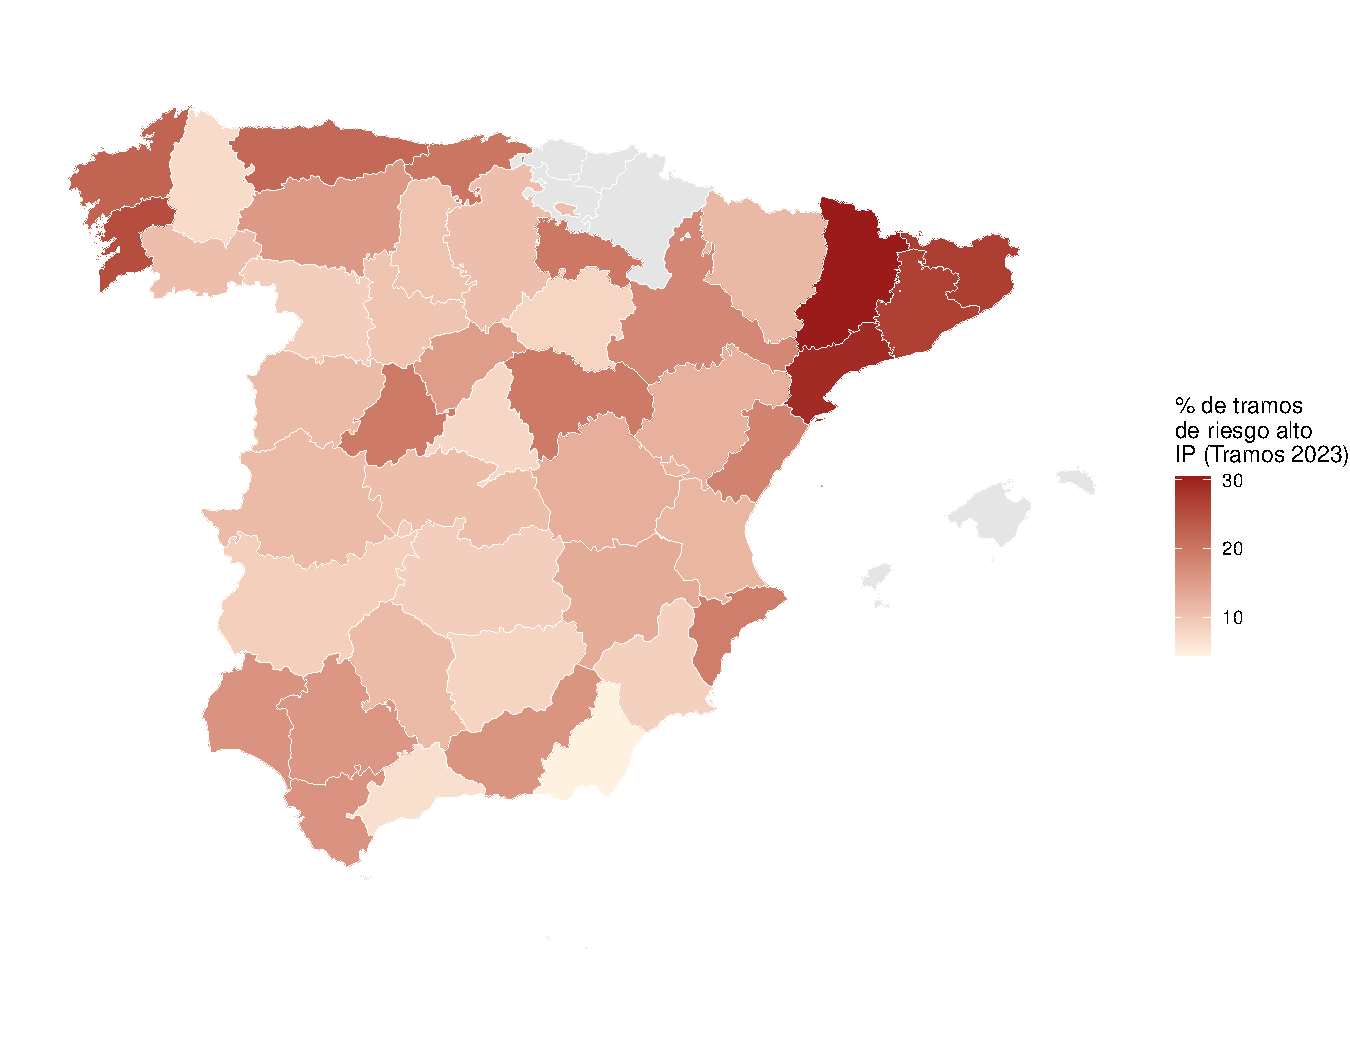
\includegraphics[width=\textwidth]{mapas/mapa_provincias_ip_2023.pdf}
    \caption{Porcentaje de tramos de riesgo alto del IP en cada provincia (Tramos 2023). En gris, provincias sin tramos de la Red de Carreteras del Estado o con menos de 30 tramos.}
    \label{fig:mapa_prov_ip_2023}
\end{figure}
 
Frente al $14.5\%$ del conjunto de los tramos, las cuatro provincias de Cataluña presentan los porcentajes más altos, de entre el $26.7\%$ (Barcelona) y el $30.5\%$ (Lleida), es decir, aproximadamente el doble de la media. Les siguen las provincias de la costa atlántica y cantábrica, como Pontevedra ($25.1\%$), A Coruña ($22.4\%$), Asturias ($21.8\%$) y Cantabria ($20.1\%$). En el extremo opuesto se encuentran Almería ($4.4\%$), Málaga ($6.7\%$), Lugo ($7.1\%$) y Madrid ($7.6\%$), con porcentajes de aproximadamente la mitad de la media. Los datos disponibles no permiten determinar la causa de estas diferencias, que pueden deberse tanto a la composición de la red de cada provincia (tipo de vía e intensidad de tráfico) como a factores no incluidos en el estudio, como el trazado de las carreteras o la climatología.
 
\vspace{0.5cm}
 
La Figura~\ref{fig:mapa_puntos_ip_2023} muestra la localización de los tramos de riesgo alto.
 
\begin{figure}[H]
    \centering
    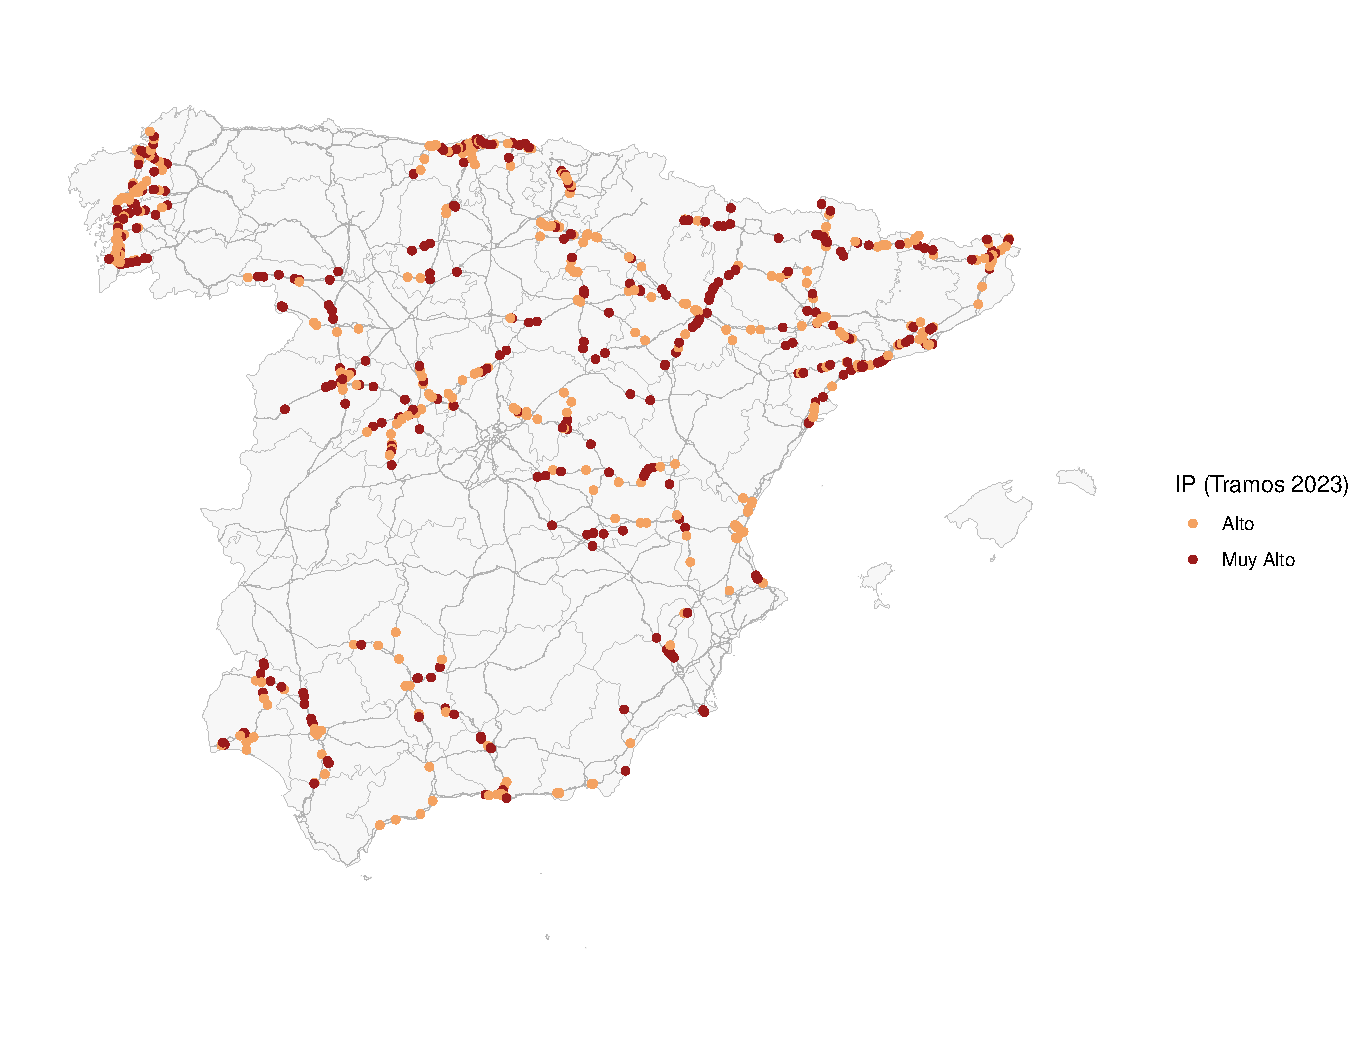
\includegraphics[width=\textwidth]{mapas/mapa_puntos_ip_2023.pdf}
    \caption{Tramos de riesgo alto del IP localizados sobre la Red de Carreteras del Estado (Tramos 2023). Se representan 653 de los 1055 tramos de riesgo alto ($61.9\%$).}
    \label{fig:mapa_puntos_ip_2023}
\end{figure}
 
Los tramos de riesgo alto no se distribuyen de forma aleatoria por la red, sino que se agrupan a lo largo de determinados corredores, especialmente en el oeste de Galicia, en la cornisa cantábrica, en el valle del Ebro y en el litoral catalán, en coherencia con el mapa por provincias.
 
\subsection{Mortalidad (IM)}
 
% ---------------------------------------------------------------------
% PENDIENTE: completar la interpretación con los porcentajes por
% provincia del IM de Tramos 2023 (print(prov_im_2023, n = 60)) y con
% lo que se observe en el mapa de puntos.
% ---------------------------------------------------------------------
 
La Figura~\ref{fig:mapa_prov_im_2023} muestra el porcentaje de tramos de riesgo alto del IM en cada provincia en 2023, y la Figura~\ref{fig:mapa_puntos_im_2023}, la localización de estos tramos.
 
\begin{figure}[H]
    \centering
    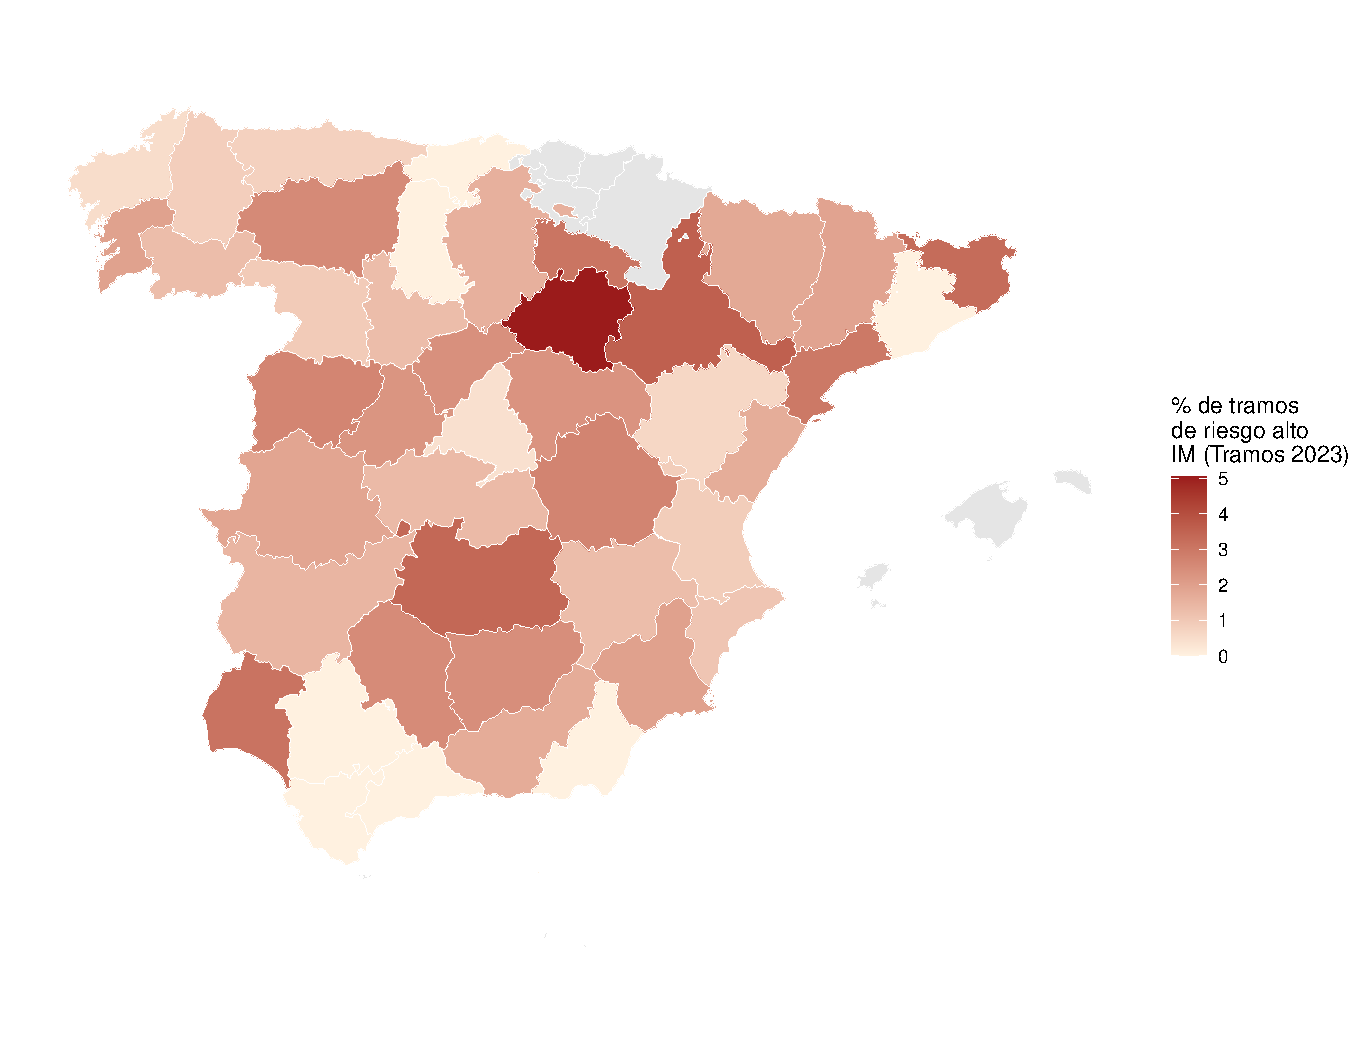
\includegraphics[width=\textwidth]{mapas/mapa_provincias_im_2023.pdf}
    \caption{Porcentaje de tramos de riesgo alto del IM en cada provincia (Tramos 2023). En gris, provincias sin tramos de la Red de Carreteras del Estado o con menos de 30 tramos.}
    \label{fig:mapa_prov_im_2023}
\end{figure}
 
\begin{figure}[H]
    \centering
    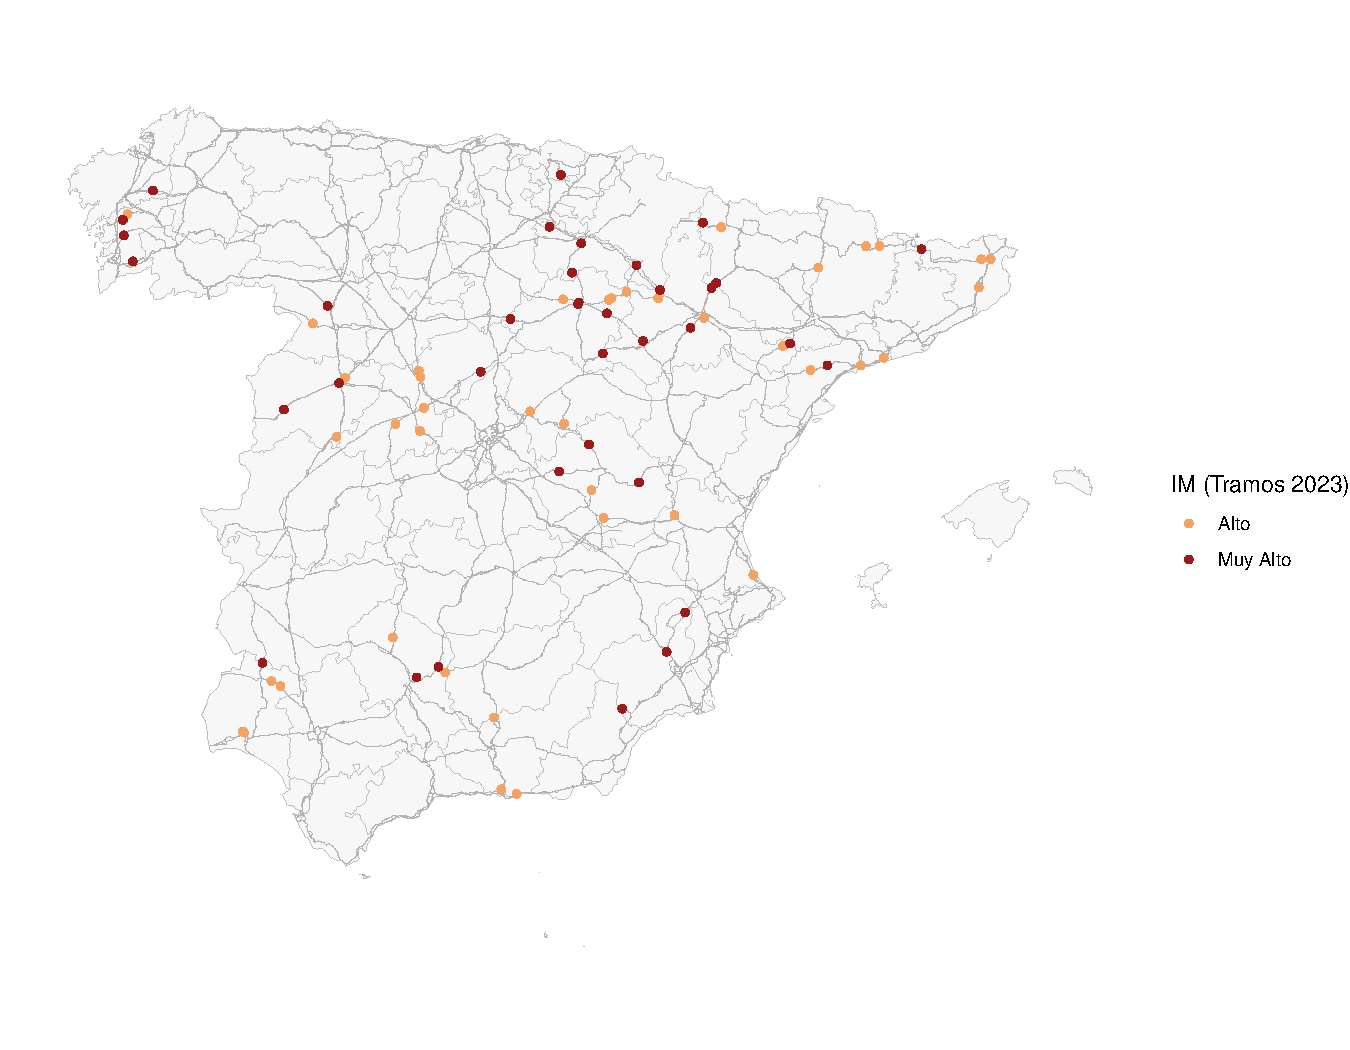
\includegraphics[width=\textwidth]{mapas/mapa_puntos_im_2023.pdf}
    \caption{Tramos de riesgo alto del IM localizados sobre la Red de Carreteras del Estado (Tramos 2023). Se representan 77 de los 120 tramos de riesgo alto ($64.2\%$).}
    \label{fig:mapa_puntos_im_2023}
\end{figure}
 
Como el IM solo clasifica como riesgo alto a 120 tramos, el porcentaje de cada provincia se basa en muy pocos casos y debe interpretarse con cautela: una diferencia de uno o dos tramos puede modificar notablemente el resultado de una provincia.
 
%%%%%%%%%%%%%%%%%%FIN CAP 7%%%%%%%%%%%%%%%%%%%%%%%%%%%%%%%%%%%%%%%%%%%%%%%

%%%%%%%%%%%%%%%%INICIO CAP 8 %%%%%%%%%%%%%%%%%%%%%%%%%%%%%%%%%%%%%%%%%%%%%%
\setcounter{chapter}{8}
\chapter*{Capítulo 8 \\ \vspace{1cm} Conclusiones}
\addcontentsline{toc}{chapter}{\protect\numberline{\thechapter}Conclusiones}

\setcounter{figure}{0}\setcounter{table}{0}

.

%%%%%%%%%%%%%%%%%%FIN CAP 8 %%%%%%%%%%%%%%%%%%%%%%%%%%%%%%%%%%%%%%%%%%%%%%%

\begin{thebibliography}{99} %ordenado alfabeticamente
%
% and use \bibitem to create references. Consult the Instructions
% for authors for reference list style.
%

\bibitem{anuarioaccidentes} Dirección General de Tráfico (2026). ``Anuario Estadístico de Accidentes 2024''. \url{https://www.dgt.es/export/sites/web-DGT/.galleries/downloads/dgt-en-cifras/publicaciones/Anuario-Estadistico-de-Accidentes/Anuario_Accidentes-_2024_accesible_metadatos_ok_20260113.pdf}.

\bibitem{mantenimientocarreteras} Revista Tráfico y Seguridad Vial (2025). ``Estado de las carreteras 2025''. Dirección General de Tráfico. \url{https://revista.dgt.es/es/noticias/nacional/2025/07JULIO/0707_EStadoCarreteras2025.shtml}

\bibitem{estrategiamovilidad} Ministerio de Transportes y Movilidad Sostenible (2020). ``Estrategia de Movilidad Segura, Sostenible y Conectada 2030''. Gobierno de España. \url{https://www.transportes.gob.es/ministerio/planes-estrategicos/esmovilidad}

\bibitem{hsm_aashto} American Association of State Highway and Transportation Officials (AASHTO) (2010). ``Highway Safety Manual''. Washington, D.C.

\bibitem{tca_dgt} Dirección General de Tráfico. ``Información sobre los tramos de concentración de accidentes''. Estrategia de Seguridad Vial 2030. Gobierno de España. \url{https://seguridadvial2030.dgt.es/practicas-de-interes/datos-y-conocimiento-para-una-gestion-basada-en-riesgos/Informacion-sobre-los-tramos-de-concentracion-de-accidentes/index.html}

\bibitem{mapatraficodgc} Ministerio de Transportes y Movilidad Sostenible. ``Mapa de Tráfico y Movilidad. Aforos''. Dirección General de Carreteras. Gobierno de España. \url{https://mapadetrafico.transportes.gob.es}

\bibitem{datamining} Han, J., Kamber, M., \& Pei, J. (2011). ``Data Mining: Concepts and Techniques'' (3.\textsuperscript{a} ed.). Morgan Kaufmann Publishers.

\bibitem{dataminingibm} International Business Machines Corporation (IBM). ``What is Data Mining?''. IBM Think Topics. \url{https://www.ibm.com/think/topics/data-mining}

\bibitem{ingenieriacarreteras} Kraemer, C., Pardillo, J. M., Rocci, S., Romana, M. G., Sánchez Blanco, V.,  del Val, M. A. (2004). ``Ingeniería de Carreteras'' (Vol. I y II). McGraw-Hill / Interamericana de España.

\bibitem{orden_accidentes} Ministerio del Interior (2014). ``Orden INT/2223/2014, de 27 de noviembre, por la que se regula la comunicación de la información al Registro Nacional de Víctimas de Accidentes de Tráfico''. Boletín Oficial del Estado, núm. 289.

\bibitem{apuntes_teoria2025} Pegalajar Jiménez, M. C. y Ruiz Jiménez, M. D. (2024). Tema 5: Perspectiva informática de la Minería de Datos. Modelos de asociación [Apuntes de clase]. Departamento de Ciencias de la Computación e Inteligencia Artificial, Universidad de Granada.

\bibitem{plan_aforos} Ministerio de Transportes y Movilidad Sostenible. ``Plan de Aforos de la Red de Carreteras del Estado''. Dirección General de Carreteras. Gobierno de España.

\bibitem{practica_asociacion} Universidad de Granada. (2024). Práctica: Análisis con Reglas de Asociación [Material de prácticas]. Departamento de Ciencias de la Computación e Inteligencia Artificial.

\bibitem{guion_arboles2024} Pegalajar Jiménez, M. C. (2024). Algoritmos de Clasificación (Parte 2: Árboles de Decisión) [Guion de prácticas]. Minería de Datos, Grado en Estadística. Departamento de Ciencias de la Computación e Inteligencia Artificial, Universidad de Granada.

\bibitem{tema3_clasificacion} Pegalajar Jiménez, M. C. (s.\,f.). Tema 3: Modelos de Clasificación [Apuntes de clase]. Departamento de Ciencias de la Computación e Inteligencia Artificial, Universidad de Granada.

\bibitem{tema2_clasificacion} Arnedo, J. (2026). Tema 2: Clasificación Estadística [Apuntes de clase]. Minería de Datos, Grado en Estadística (curso 2025-2026). Departamento de Estadística e Investigación Operativa, Universidad de Granada.

\bibitem{quinlan1986} Quinlan, J. R. (1986). Induction of decision trees. Machine Learning, 1(1), 81--106.

\bibitem{quinlan1993} Quinlan, J. R. (1993). C4.5: Programs for Machine Learning. Morgan Kaufmann.


\end{thebibliography}
\newpage
%%%%%%%%%%%%%%%%%%%%%%%%%%% ANEXO %%%%%%%%%%%%%%%%%%%%%%%%%%%
% \appendix %se me sale fuera de la pagina
\chapter*{Anexo}
\addcontentsline{toc}{chapter}{Anexo}
\setcounter{table}{0}
\renewcommand{\thetable}{A.\arabic{table}}

\section*{Tablas de la búsqueda de parámetros}
A continuación se recogen los resultados de la búsqueda de parámetros con balanceo en las siete bases de datos restantes, con el mismo formato que la Tabla~\ref{tab:busqueda_ip_2023}.
 
\subsection*{Base de Datos de Tramos IM 2023}
 
\begin{table}[H]
\centering
\small
\setlength{\tabcolsep}{4pt}
\begin{tabular}{r|cccc}
\toprule
 & \multicolumn{4}{c}{\textbf{minbucket}} \\
\cmidrule(lr){2-5}
\textbf{cp} & \textbf{20} & \textbf{40} & \textbf{80} & \textbf{120} \\
\midrule
0.001 & \shortstack{0.5156~(0.0361)\\ 104 hojas} & \shortstack{0.5350~(0.0465)\\ 69 hojas} & \shortstack{0.5320~(0.0750)\\ 38 hojas} & \shortstack{0.5605~(0.0824)\\ 24 hojas} \\[4pt]
0.0025 & \shortstack{0.5169~(0.0351)\\ 84 hojas} & \shortstack{0.5121~(0.0540)\\ 63 hojas} & \shortstack{0.5400~(0.0897)\\ 37 hojas} & \shortstack{0.5636~(0.0817)\\ 23 hojas} \\[4pt]
0.005 & \shortstack{0.5118~(0.0517)\\ 55 hojas} & \shortstack{0.5004~(0.0649)\\ 55 hojas} & \shortstack{0.5482~(0.0880)\\ 31 hojas} & \shortstack{0.5704~(0.0784)\\ 23 hojas} \\[4pt]
0.01 & \shortstack{0.5124~(0.0869)\\ 19 hojas} & \shortstack{0.5258~(0.0747)\\ 21 hojas} & \shortstack{0.5549~(0.0818)\\ 21 hojas} & \shortstack{0.5820~(0.0793)\\ 17 hojas} \\[4pt]
0.02 & \shortstack{0.6073~(0.0784)\\ 5 hojas} & \shortstack{0.6359~(0.0701)\\ 5 hojas} & \shortstack{0.6047~(0.0787)\\ 5 hojas} & \shortstack{0.6146~(0.0665)\\ 5 hojas} \\[4pt]
0.03 & \shortstack{0.6396~(0.0598)\\ 5 hojas} & \shortstack{0.6391~(0.0618)\\ 5 hojas} & \shortstack{\textbf{0.6472}$^{*}$~\textbf{(0.0577)}\\ \textbf{5 hojas}} & \shortstack{0.6445~(0.0659)\\ 5 hojas} \\[4pt]
0.05 & \shortstack{0.5892~(0.0827)\\ 1 hoja} & \shortstack{0.5776~(0.0791)\\ 1 hoja} & \shortstack{0.5993~(0.0850)\\ 1 hoja} & \shortstack{0.5735~(0.0811)\\ 1 hoja} \\[4pt]
\bottomrule
\end{tabular}
\caption{Resultados de la búsqueda de parámetros con balanceo en la base de Tramos 2023, IM.}
\label{tab:busqueda_im_2023}
\end{table}
 
\vspace{0.3cm}
 
\subsection*{Base de Datos de Tramos IP 2024}
 
\begin{table}[H]
\centering
\small
\setlength{\tabcolsep}{4pt}
\begin{tabular}{r|cccc}
\toprule
 & \multicolumn{4}{c}{\textbf{minbucket}} \\
\cmidrule(lr){2-5}
\textbf{cp} & \textbf{20} & \textbf{40} & \textbf{80} & \textbf{120} \\
\midrule
0.001 & \shortstack{0.6625~(0.0181)\\ 103 hojas} & \shortstack{0.6677$^{*}$~(0.0204)\\ 64 hojas} & \shortstack{0.6642~(0.0199)\\ 24 hojas} & \shortstack{0.6638~(0.0167)\\ 20 hojas} \\[4pt]
0.0025 & \shortstack{0.6607~(0.0188)\\ 50 hojas} & \shortstack{0.6651~(0.0172)\\ 39 hojas} & \shortstack{0.6652~(0.0180)\\ 22 hojas} & \shortstack{0.6625~(0.0165)\\ 20 hojas} \\[4pt]
0.005 & \shortstack{0.6608~(0.0169)\\ 22 hojas} & \shortstack{0.6626~(0.0188)\\ 24 hojas} & \shortstack{0.6655~(0.0149)\\ 21 hojas} & \shortstack{0.6639~(0.0133)\\ 18 hojas} \\[4pt]
0.01 & \shortstack{0.6592~(0.0142)\\ 8 hojas} & \shortstack{0.6598~(0.0143)\\ 8 hojas} & \shortstack{0.6611~(0.0155)\\ 3 hojas} & \shortstack{\textbf{0.6619}~\textbf{(0.0136)}\\ \textbf{3 hojas}} \\[4pt]
0.02 & \shortstack{0.6187~(0.0688)\\ 3 hojas} & \shortstack{0.6390~(0.0540)\\ 3 hojas} & \shortstack{0.6204~(0.0699)\\ 3 hojas} & \shortstack{0.6273~(0.0657)\\ 3 hojas} \\[4pt]
0.03 & \shortstack{0.5232~(0.0543)\\ 1 hoja} & \shortstack{0.5302~(0.0617)\\ 1 hoja} & \shortstack{0.5415~(0.0680)\\ 1 hoja} & \shortstack{0.5171~(0.0474)\\ 1 hoja} \\[4pt]
0.05 & \shortstack{0.5000~(0.0000)\\ 1 hoja} & \shortstack{0.5000~(0.0000)\\ 1 hoja} & \shortstack{0.5000~(0.0000)\\ 1 hoja} & \shortstack{0.5000~(0.0000)\\ 1 hoja} \\[4pt]
\bottomrule
\end{tabular}
\caption{Resultados de la búsqueda de parámetros con balanceo en la base de Tramos 2024, IP.}
\label{tab:busqueda_ip_2024}
\end{table}
 
\vspace{0.1cm}
 
\subsection*{Base de Datos de Tramos IM 2024}
 
\begin{table}[H]
\centering
\small
\setlength{\tabcolsep}{4pt}
\begin{tabular}{r|cccc}
\toprule
 & \multicolumn{4}{c}{\textbf{minbucket}} \\
\cmidrule(lr){2-5}
\textbf{cp} & \textbf{20} & \textbf{40} & \textbf{80} & \textbf{120} \\
\midrule
0.001 & \shortstack{0.5159~(0.0374)\\ 89 hojas} & \shortstack{0.5283~(0.0631)\\ 58 hojas} & \shortstack{0.5713~(0.0724)\\ 29 hojas} & \shortstack{0.5887~(0.0570)\\ 26 hojas} \\[4pt]
0.0025 & \shortstack{0.5214~(0.0414)\\ 89 hojas} & \shortstack{0.5315~(0.0507)\\ 57 hojas} & \shortstack{0.5665~(0.0706)\\ 28 hojas} & \shortstack{0.5983~(0.0489)\\ 25 hojas} \\[4pt]
0.005 & \shortstack{0.5228~(0.0530)\\ 60 hojas} & \shortstack{0.5181~(0.0612)\\ 45 hojas} & \shortstack{0.5811~(0.0595)\\ 27 hojas} & \shortstack{0.5890~(0.0570)\\ 23 hojas} \\[4pt]
0.01 & \shortstack{0.5371~(0.0969)\\ 25 hojas} & \shortstack{0.5318~(0.1102)\\ 25 hojas} & \shortstack{0.5898~(0.0807)\\ 20 hojas} & \shortstack{0.6071~(0.0669)\\ 19 hojas} \\[4pt]
0.02 & \shortstack{0.6182~(0.0682)\\ 4 hojas} & \shortstack{0.6105~(0.0738)\\ 4 hojas} & \shortstack{\textbf{0.6208}~\textbf{(0.0836)}\\ \textbf{4 hojas}} & \shortstack{0.6142~(0.0758)\\ 4 hojas} \\[4pt]
0.03 & \shortstack{0.6191~(0.0769)\\ 4 hojas} & \shortstack{0.6111~(0.0754)\\ 4 hojas} & \shortstack{0.6218$^{*}$~(0.0729)\\ 4 hojas} & \shortstack{0.6141~(0.0809)\\ 4 hojas} \\[4pt]
0.05 & \shortstack{0.5725~(0.0733)\\ 3 hojas} & \shortstack{0.5639~(0.0661)\\ 3 hojas} & \shortstack{0.5950~(0.0664)\\ 3 hojas} & \shortstack{0.5701~(0.0636)\\ 3 hojas} \\[4pt]
\bottomrule
\end{tabular}
\caption{Resultados de la búsqueda de parámetros con balanceo en la base de Tramos 2024, IM.}
\label{tab:busqueda_im_2024}
\end{table}
 
\vspace{0.1cm}
 
\subsection*{Base de Datos de Accidentes IP 2023}
 
\begin{table}[H]
\centering
\small
\setlength{\tabcolsep}{4pt}
\begin{tabular}{r|cccc}
\toprule
 & \multicolumn{4}{c}{\textbf{minbucket}} \\
\cmidrule(lr){2-5}
\textbf{cp} & \textbf{20} & \textbf{40} & \textbf{80} & \textbf{120} \\
\midrule
0.001 & \shortstack{0.7825~(0.0492)\\ 45 hojas} & \shortstack{0.8006~(0.0438)\\ 27 hojas} & \shortstack{0.8047~(0.0395)\\ 13 hojas} & \shortstack{0.8039~(0.0497)\\ 12 hojas} \\[4pt]
0.0025 & \shortstack{0.7890~(0.0581)\\ 37 hojas} & \shortstack{0.8000~(0.0422)\\ 27 hojas} & \shortstack{0.7984~(0.0462)\\ 13 hojas} & \shortstack{0.8092$^{*}$~(0.0383)\\ 12 hojas} \\[4pt]
0.005 & \shortstack{0.7881~(0.0477)\\ 16 hojas} & \shortstack{0.7891~(0.0353)\\ 17 hojas} & \shortstack{\textbf{0.8010}~\textbf{(0.0311)}\\ \textbf{2 hojas}} & \shortstack{0.7980~(0.0345)\\ 2 hojas} \\[4pt]
0.01 & \shortstack{0.7889~(0.0303)\\ 2 hojas} & \shortstack{0.7862~(0.0287)\\ 2 hojas} & \shortstack{0.7854~(0.0315)\\ 2 hojas} & \shortstack{0.7878~(0.0286)\\ 2 hojas} \\[4pt]
0.02 & \shortstack{0.7872~(0.0317)\\ 2 hojas} & \shortstack{0.7872~(0.0317)\\ 2 hojas} & \shortstack{0.7872~(0.0317)\\ 2 hojas} & \shortstack{0.7872~(0.0317)\\ 2 hojas} \\[4pt]
0.03 & \shortstack{0.7872~(0.0317)\\ 2 hojas} & \shortstack{0.7872~(0.0317)\\ 2 hojas} & \shortstack{0.7872~(0.0317)\\ 2 hojas} & \shortstack{0.7872~(0.0317)\\ 2 hojas} \\[4pt]
0.05 & \shortstack{0.7872~(0.0317)\\ 2 hojas} & \shortstack{0.7872~(0.0317)\\ 2 hojas} & \shortstack{0.7872~(0.0317)\\ 2 hojas} & \shortstack{0.7872~(0.0317)\\ 2 hojas} \\[4pt]
\bottomrule
\end{tabular}
\caption{Resultados de la búsqueda de parámetros con balanceo en la base de Accidentes 2023, IP.}
\label{tab:busqueda_acc_ip_2023}
\end{table}
 
\vspace{0.0cm}
 
\subsection*{Base de Datos de Accidentes IM 2023}
 
\begin{table}[H]
\centering
\small
\setlength{\tabcolsep}{4pt}
\begin{tabular}{r|cccc}
\toprule
 & \multicolumn{4}{c}{\textbf{minbucket}} \\
\cmidrule(lr){2-5}
\textbf{cp} & \textbf{20} & \textbf{40} & \textbf{80} & \textbf{120} \\
\midrule
0.001 & \shortstack{0.5834~(0.0966)\\ 88 hojas} & \shortstack{0.6750~(0.0899)\\ 54 hojas} & \shortstack{0.7164~(0.0566)\\ 37 hojas} & \shortstack{0.7531~(0.0454)\\ 18 hojas} \\[4pt]
0.0025 & \shortstack{0.5761~(0.0901)\\ 77 hojas} & \shortstack{0.6712~(0.0948)\\ 45 hojas} & \shortstack{0.7240~(0.0641)\\ 27 hojas} & \shortstack{0.7524~(0.0603)\\ 17 hojas} \\[4pt]
0.005 & \shortstack{0.6320~(0.0883)\\ 28 hojas} & \shortstack{0.6688~(0.0873)\\ 28 hojas} & \shortstack{0.7209~(0.0736)\\ 27 hojas} & \shortstack{0.7439~(0.0557)\\ 16 hojas} \\[4pt]
0.01 & \shortstack{0.7309~(0.0767)\\ 7 hojas} & \shortstack{0.7358~(0.0734)\\ 10 hojas} & \shortstack{0.7346~(0.0742)\\ 9 hojas} & \shortstack{0.7519~(0.0525)\\ 7 hojas} \\[4pt]
0.02 & \shortstack{0.7522~(0.0500)\\ 4 hojas} & \shortstack{0.7583~(0.0485)\\ 4 hojas} & \shortstack{0.7587$^{*}$~(0.0564)\\ 4 hojas} & \shortstack{0.7584~(0.0562)\\ 4 hojas} \\[4pt]
0.03 & \shortstack{0.7556~(0.0634)\\ 3 hojas} & \shortstack{0.7495~(0.0507)\\ 3 hojas} & \shortstack{0.7518~(0.0577)\\ 3 hojas} & \shortstack{0.7537~(0.0549)\\ 3 hojas} \\[4pt]
0.05 & \shortstack{0.7416~(0.0476)\\ 3 hojas} & \shortstack{0.7468~(0.0527)\\ 3 hojas} & \shortstack{0.7469~(0.0610)\\ 3 hojas} & \shortstack{\textbf{0.7575}~\textbf{(0.0623)}\\ \textbf{3 hojas}} \\[4pt]
\bottomrule
\end{tabular}
\caption{Resultados de la búsqueda de parámetros con balanceo en la base de Accidentes 2023, IM.}
\label{tab:busqueda_acc_im_2023}
\end{table}
 
\vspace{0.0cm}
 
\subsection*{Base de Datos de Accidentes IP 2024}
 
\begin{table}[H]
\centering
\small
\setlength{\tabcolsep}{4pt}
\begin{tabular}{r|cccc}
\toprule
 & \multicolumn{4}{c}{\textbf{minbucket}} \\
\cmidrule(lr){2-5}
\textbf{cp} & \textbf{20} & \textbf{40} & \textbf{80} & \textbf{120} \\
\midrule
0.001 & \shortstack{0.8138~(0.0341)\\ 45 hojas} & \shortstack{0.8268~(0.0384)\\ 29 hojas} & \shortstack{0.8179~(0.0436)\\ 7 hojas} & \shortstack{0.8273$^{*}$~(0.0343)\\ 6 hojas} \\[4pt]
0.0025 & \shortstack{0.8057~(0.0401)\\ 24 hojas} & \shortstack{0.8117~(0.0317)\\ 23 hojas} & \shortstack{0.8191~(0.0366)\\ 7 hojas} & \shortstack{0.8230~(0.0336)\\ 4 hojas} \\[4pt]
0.005 & \shortstack{0.8118~(0.0410)\\ 8 hojas} & \shortstack{0.8155~(0.0355)\\ 6 hojas} & \shortstack{0.8220~(0.0281)\\ 7 hojas} & \shortstack{\textbf{0.8188}~\textbf{(0.0321)}\\ \textbf{2 hojas}} \\[4pt]
0.01 & \shortstack{0.8140~(0.0320)\\ 2 hojas} & \shortstack{0.8092~(0.0333)\\ 2 hojas} & \shortstack{0.8090~(0.0309)\\ 2 hojas} & \shortstack{0.8071~(0.0289)\\ 2 hojas} \\[4pt]
0.02 & \shortstack{0.8051~(0.0276)\\ 2 hojas} & \shortstack{0.8050~(0.0277)\\ 2 hojas} & \shortstack{0.8050~(0.0277)\\ 2 hojas} & \shortstack{0.8052~(0.0276)\\ 2 hojas} \\[4pt]
0.03 & \shortstack{0.8049~(0.0279)\\ 2 hojas} & \shortstack{0.8049~(0.0279)\\ 2 hojas} & \shortstack{0.8049~(0.0279)\\ 2 hojas} & \shortstack{0.8049~(0.0279)\\ 2 hojas} \\[4pt]
0.05 & \shortstack{0.8049~(0.0279)\\ 2 hojas} & \shortstack{0.8049~(0.0279)\\ 2 hojas} & \shortstack{0.8049~(0.0279)\\ 2 hojas} & \shortstack{0.8049~(0.0279)\\ 2 hojas} \\[4pt]
\bottomrule
\end{tabular}
\caption{Resultados de la búsqueda de parámetros con balanceo en la base de Accidentes 2024, IP.}
\label{tab:busqueda_acc_ip_2024}
\end{table}
 
\vspace{0.1cm}
 
\subsection*{Base de Datos de Accidentes IM 2024}
 
\begin{table}[H]
\centering
\small
\setlength{\tabcolsep}{4pt}
\begin{tabular}{r|cccc}
\toprule
 & \multicolumn{4}{c}{\textbf{minbucket}} \\
\cmidrule(lr){2-5}
\textbf{cp} & \textbf{20} & \textbf{40} & \textbf{80} & \textbf{120} \\
\midrule
0.001 & \shortstack{0.6038~(0.0716)\\ 94 hojas} & \shortstack{0.6405~(0.0688)\\ 69 hojas} & \shortstack{0.6438~(0.0679)\\ 42 hojas} & \shortstack{0.6456~(0.0610)\\ 32 hojas} \\[4pt]
0.0025 & \shortstack{0.6254~(0.0752)\\ 71 hojas} & \shortstack{0.6474~(0.0599)\\ 64 hojas} & \shortstack{0.6307~(0.0598)\\ 40 hojas} & \shortstack{0.6452~(0.0539)\\ 26 hojas} \\[4pt]
0.005 & \shortstack{0.6244~(0.0844)\\ 40 hojas} & \shortstack{0.6476~(0.0673)\\ 36 hojas} & \shortstack{0.6324~(0.0799)\\ 31 hojas} & \shortstack{0.6539~(0.0604)\\ 24 hojas} \\[4pt]
0.01 & \shortstack{0.6356~(0.0544)\\ 16 hojas} & \shortstack{0.6458~(0.0635)\\ 16 hojas} & \shortstack{0.6465~(0.0521)\\ 16 hojas} & \shortstack{0.6480~(0.0548)\\ 12 hojas} \\[4pt]
0.02 & \shortstack{0.6491~(0.0439)\\ 3 hojas} & \shortstack{0.6534~(0.0451)\\ 3 hojas} & \shortstack{0.6544~(0.0490)\\ 3 hojas} & \shortstack{0.6518~(0.0512)\\ 3 hojas} \\[4pt]
0.03 & \shortstack{0.6633~(0.0479)\\ 2 hojas} & \shortstack{0.6606~(0.0563)\\ 2 hojas} & \shortstack{0.6680~(0.0591)\\ 2 hojas} & \shortstack{0.6674~(0.0540)\\ 2 hojas} \\[4pt]
0.05 & \shortstack{\textbf{0.6681}$^{*}$~\textbf{(0.0474)}\\ \textbf{2 hojas}} & \shortstack{0.6644~(0.0469)\\ 2 hojas} & \shortstack{0.6641~(0.0478)\\ 2 hojas} & \shortstack{0.6671~(0.0509)\\ 2 hojas} \\[4pt]
\bottomrule
\end{tabular}
\caption{Resultados de la búsqueda de parámetros con balanceo en la base de Accidentes 2024, IM.}
\label{tab:busqueda_acc_im_2024}
\end{table}
 
\vspace{0.5cm}

\section*{Mapas de la distribución geográfica del riesgo}
A continuación se recogen los mapas por provincias y de puntos del resto de bases de datos, elaborados con el mismo procedimiento que los del apartado~7.4. En las bases de Accidentes, el porcentaje de cada provincia se refiere a los puntos kilométricos con siniestros, por lo que no es directamente comparable con el de las bases de Tramos.
 
\begin{figure}[H]
    \centering
    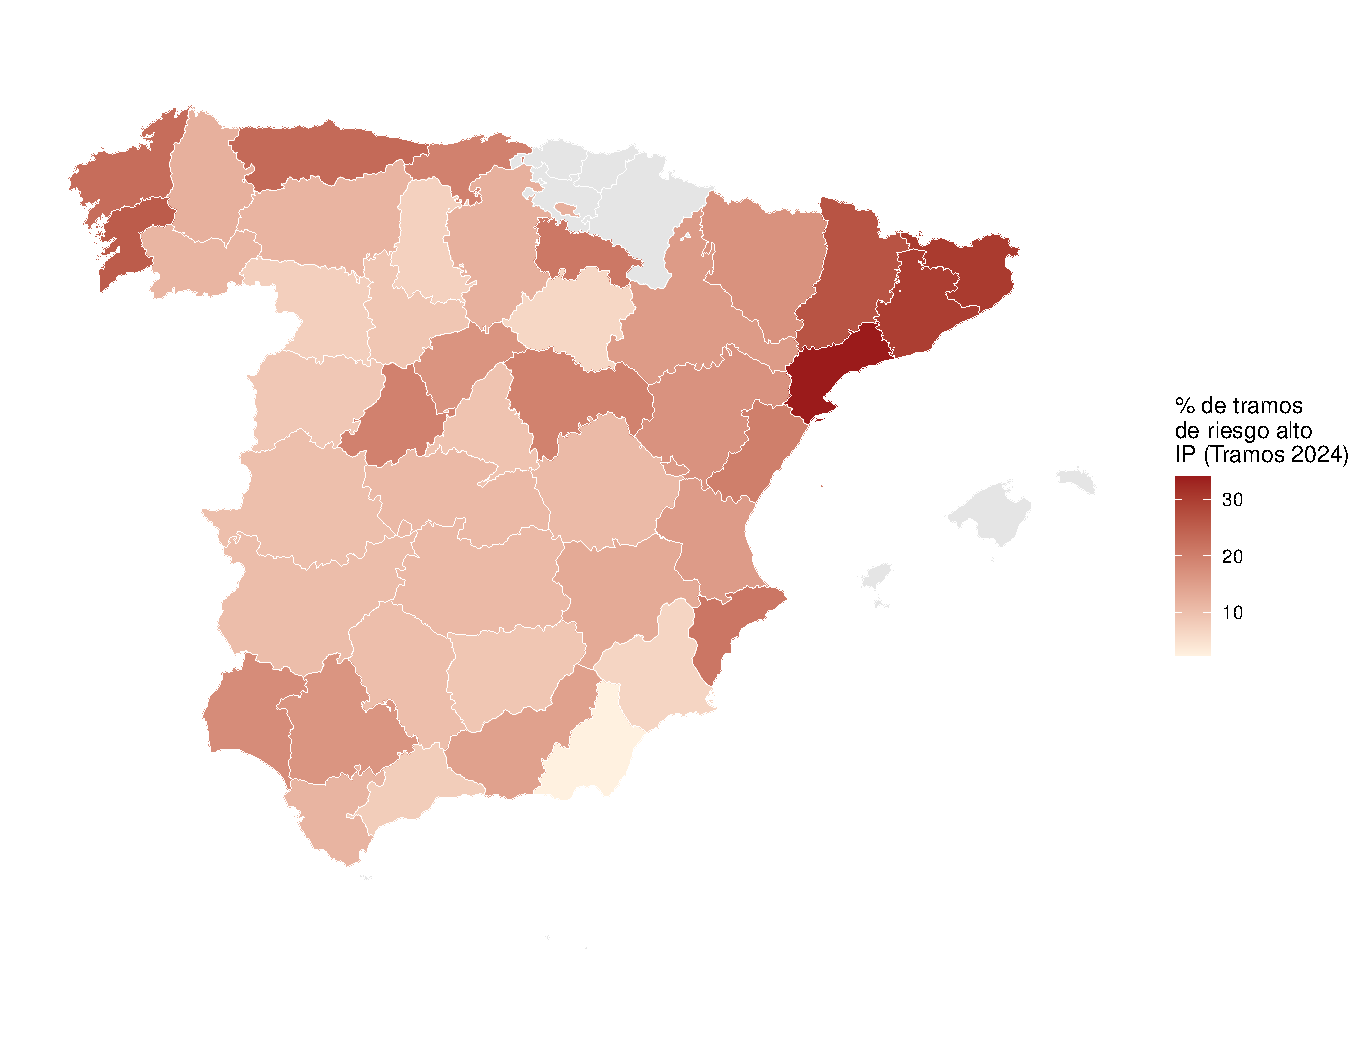
\includegraphics[width=0.85\textwidth]{mapas/mapa_provincias_ip_2024.pdf}
    \caption{Porcentaje de tramos de riesgo alto del IP en cada provincia (Tramos 2024). En gris, provincias sin registros de la Red de Carreteras del Estado o con menos de 30 registros.}
    \label{fig:mapa_prov_ip_2024}
\end{figure}
 
\begin{figure}[H]
    \centering
    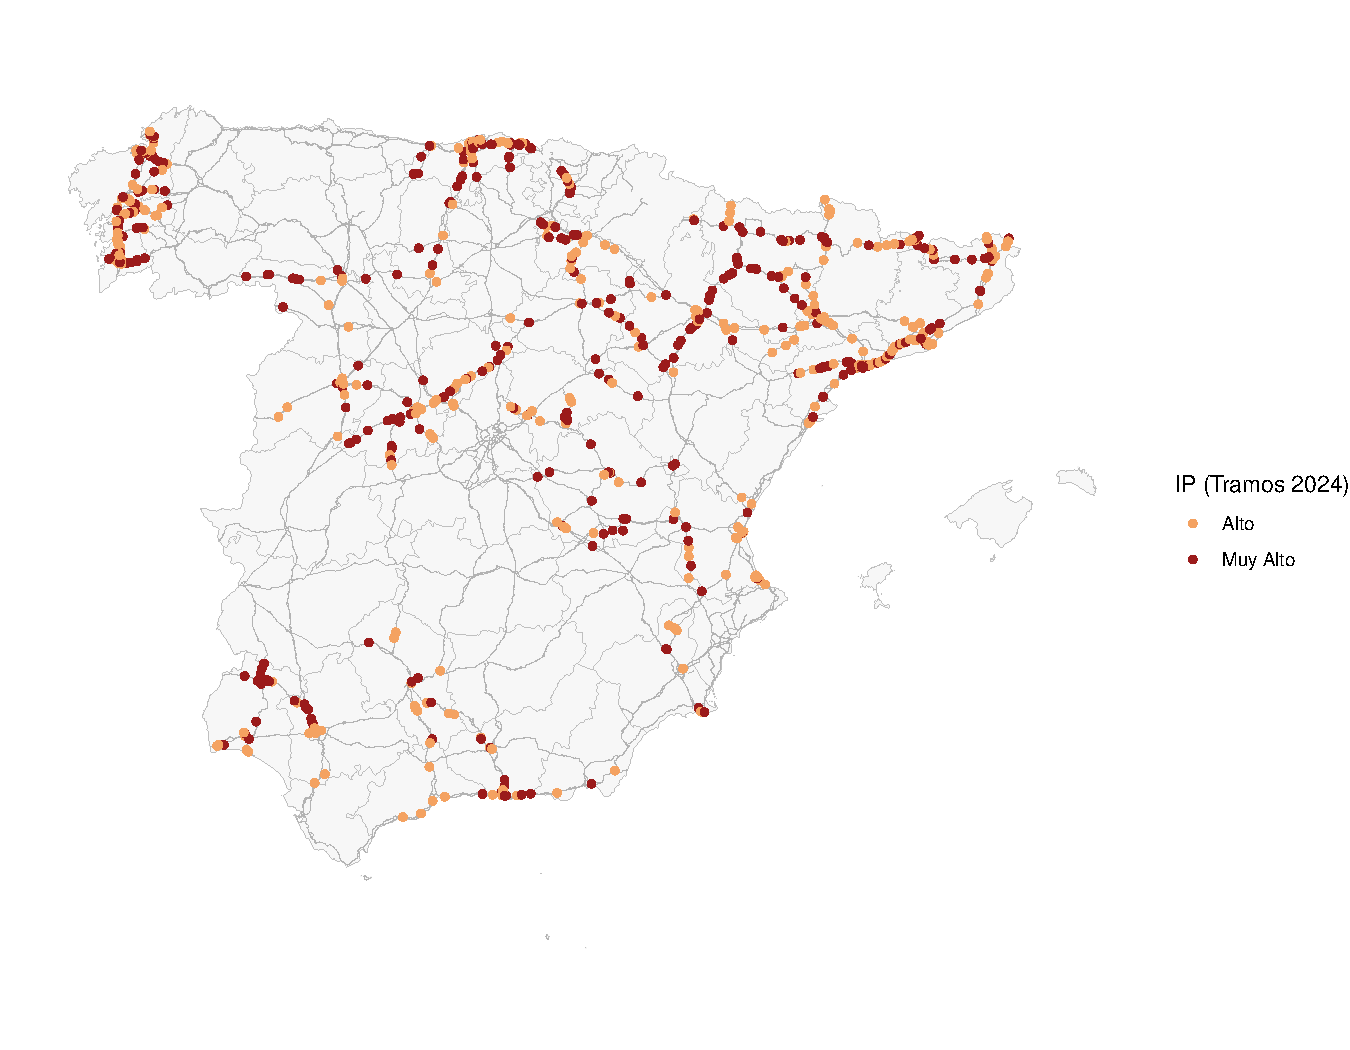
\includegraphics[width=0.85\textwidth]{mapas/mapa_puntos_ip_2024.pdf}
    \caption{Tramos de riesgo alto del IP localizados sobre la Red de Carreteras del Estado (Tramos 2024). Se representan 662 de los 1088 tramos de riesgo alto ($60.8\%$).}
    \label{fig:mapa_puntos_ip_2024}
\end{figure}
 
\begin{figure}[H]
    \centering
    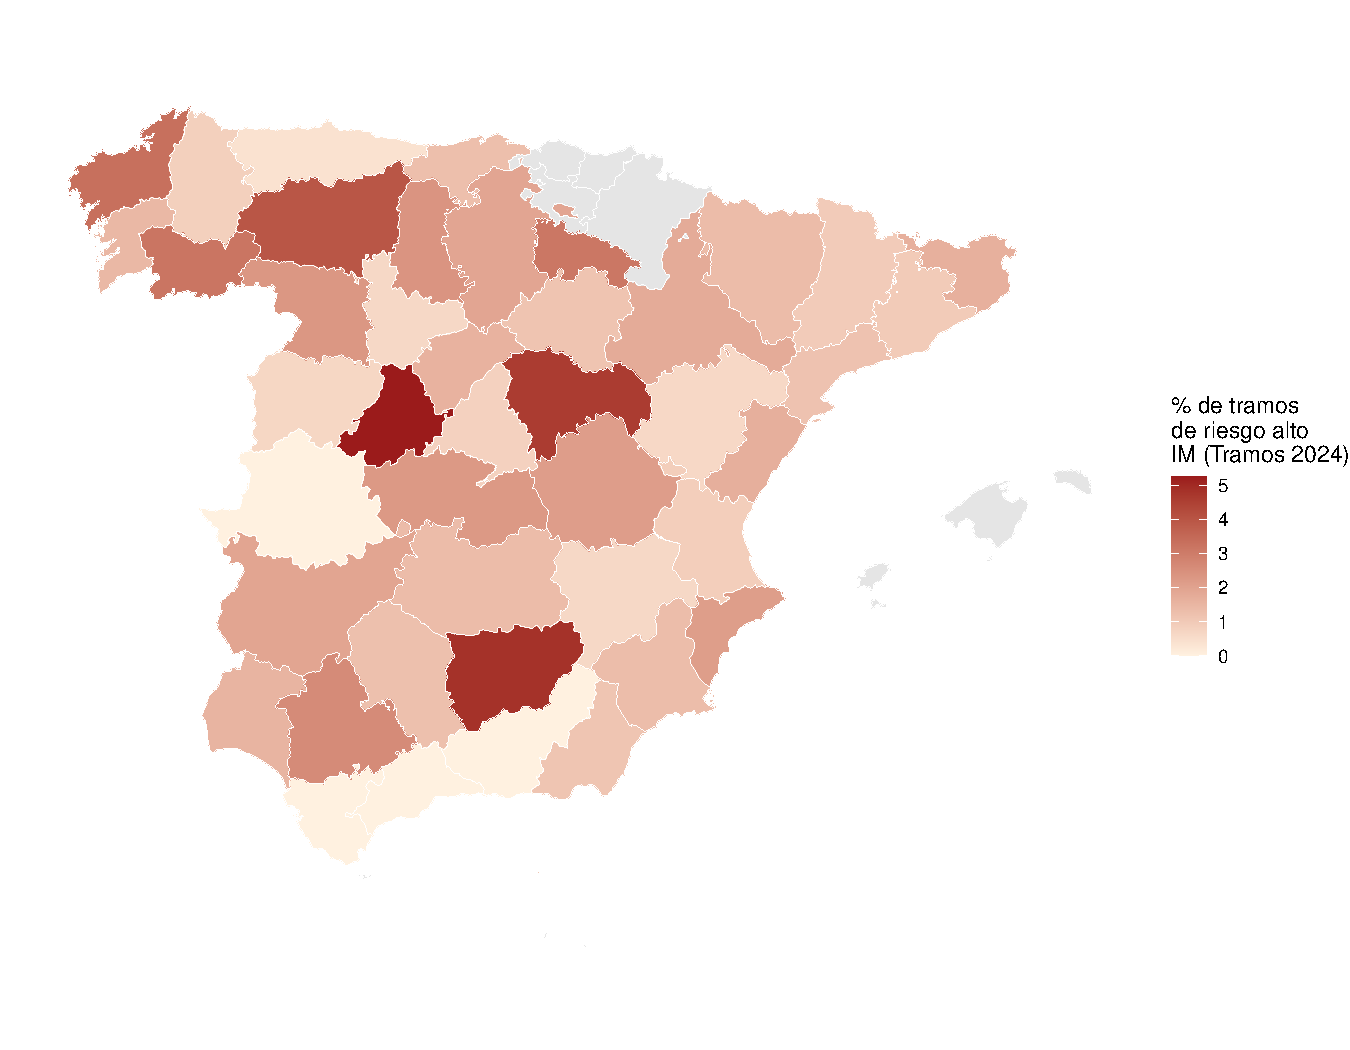
\includegraphics[width=0.85\textwidth]{mapas/mapa_provincias_im_2024.pdf}
    \caption{Porcentaje de tramos de riesgo alto del IM en cada provincia (Tramos 2024).}
    \label{fig:mapa_prov_im_2024}
\end{figure}
 
\begin{figure}[H]
    \centering
    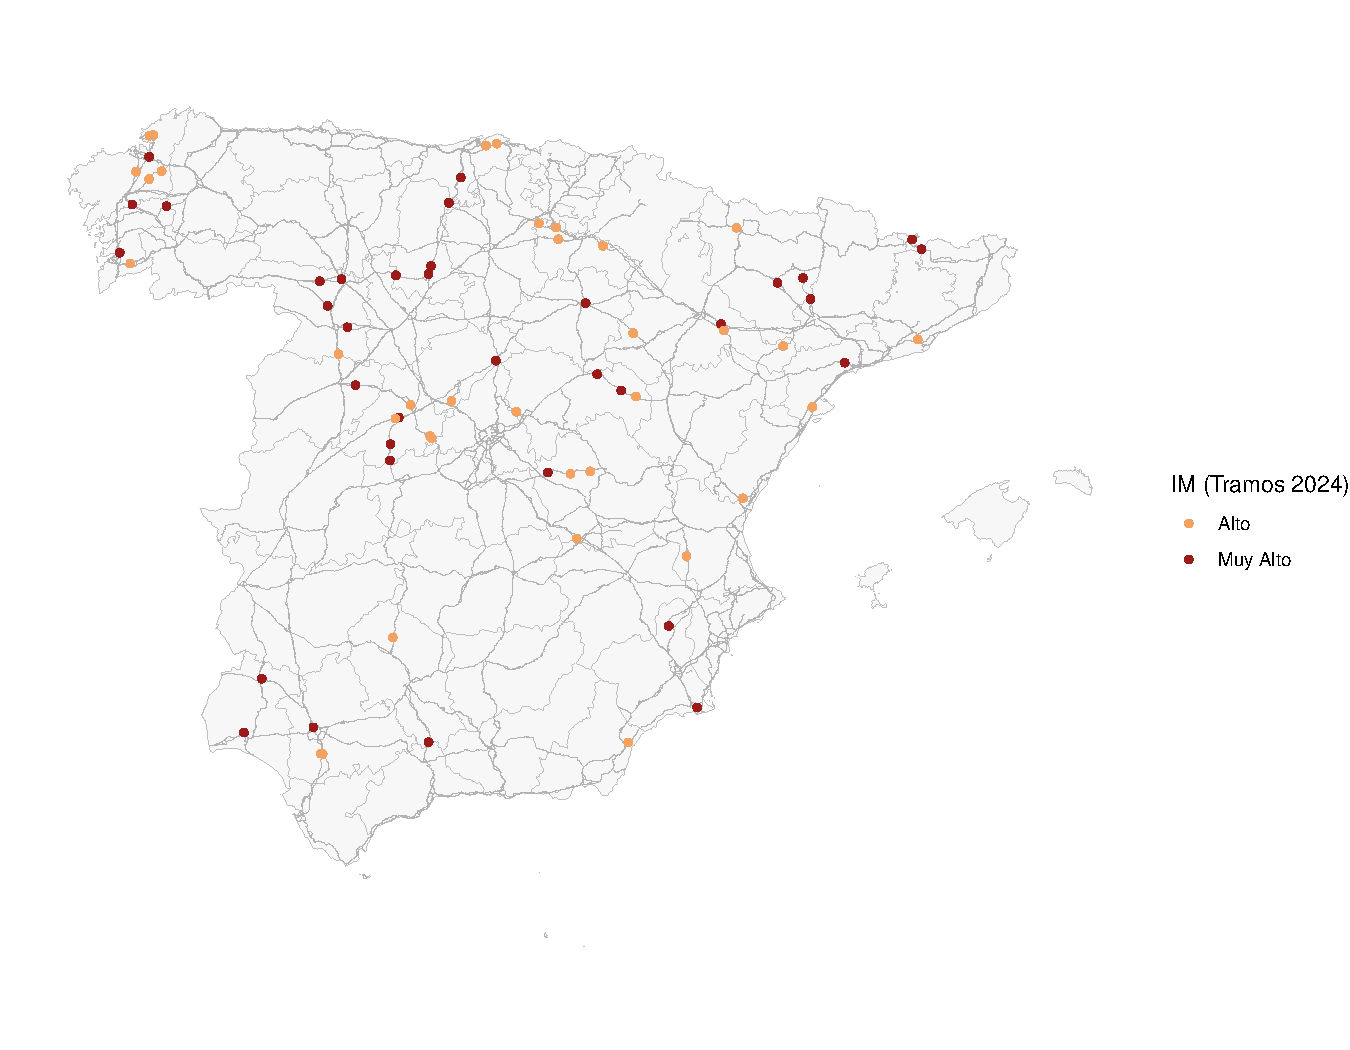
\includegraphics[width=0.85\textwidth]{mapas/mapa_puntos_im_2024.pdf}
    \caption{Tramos de riesgo alto del IM localizados sobre la Red de Carreteras del Estado (Tramos 2024). Se representan 70 de los 123 tramos de riesgo alto ($56.9\%$).}
    \label{fig:mapa_puntos_im_2024}
\end{figure}
 
\begin{figure}[H]
    \centering
    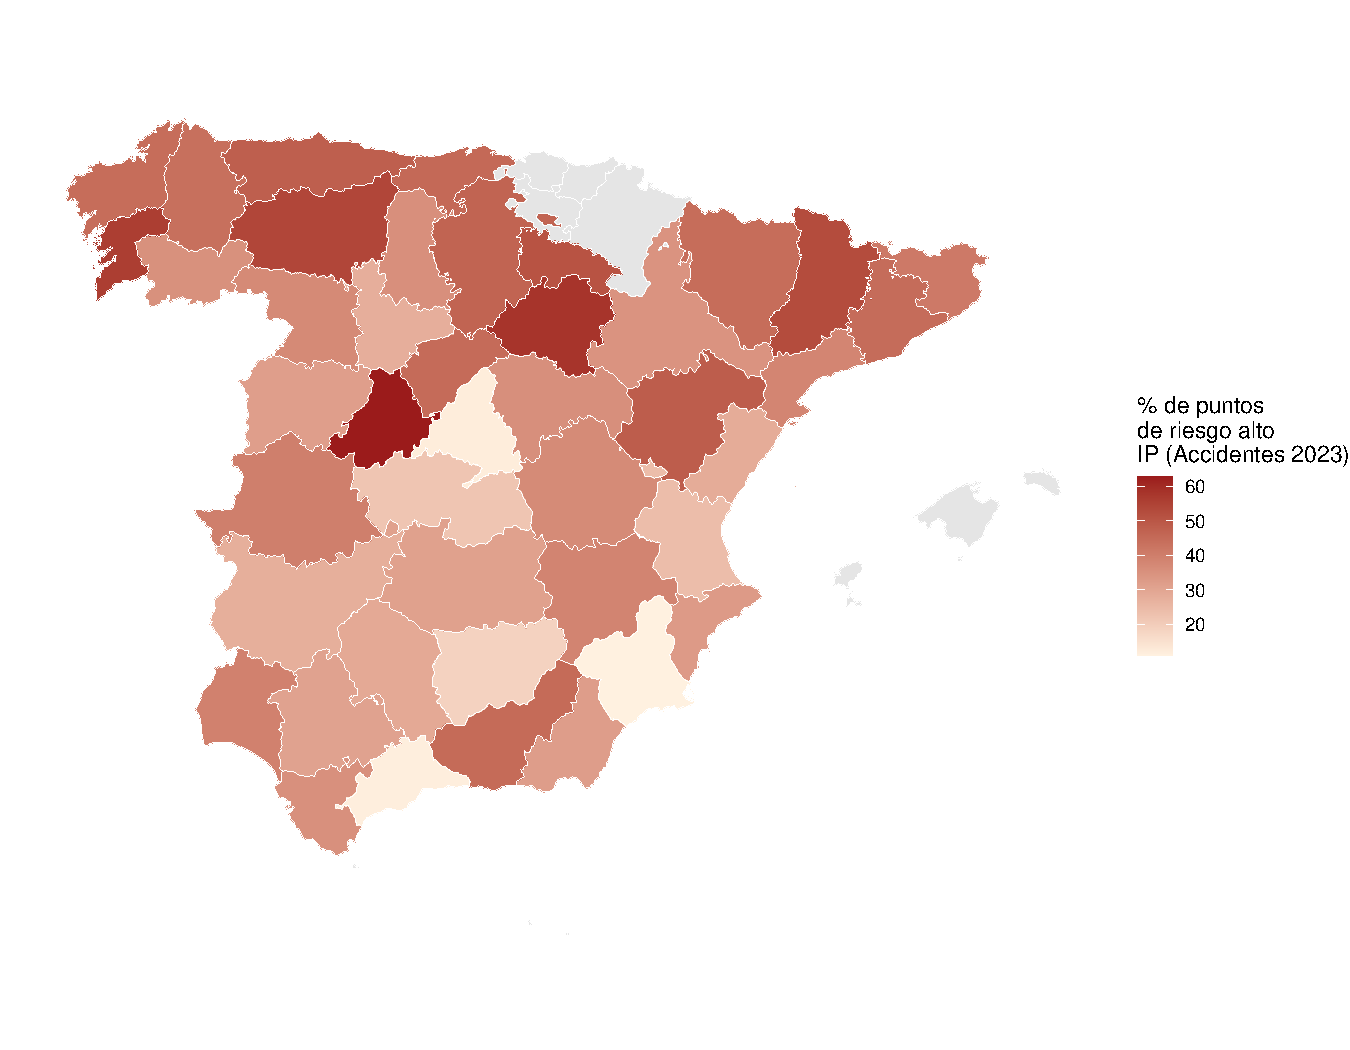
\includegraphics[width=0.85\textwidth]{mapas/mapa_provincias_acc_ip_2023.pdf}
    \caption{Porcentaje de puntos kilométricos de riesgo alto del IP en cada provincia (Accidentes 2023).}
    \label{fig:mapa_prov_acc_ip_2023}
\end{figure}
 
\begin{figure}[H]
    \centering
    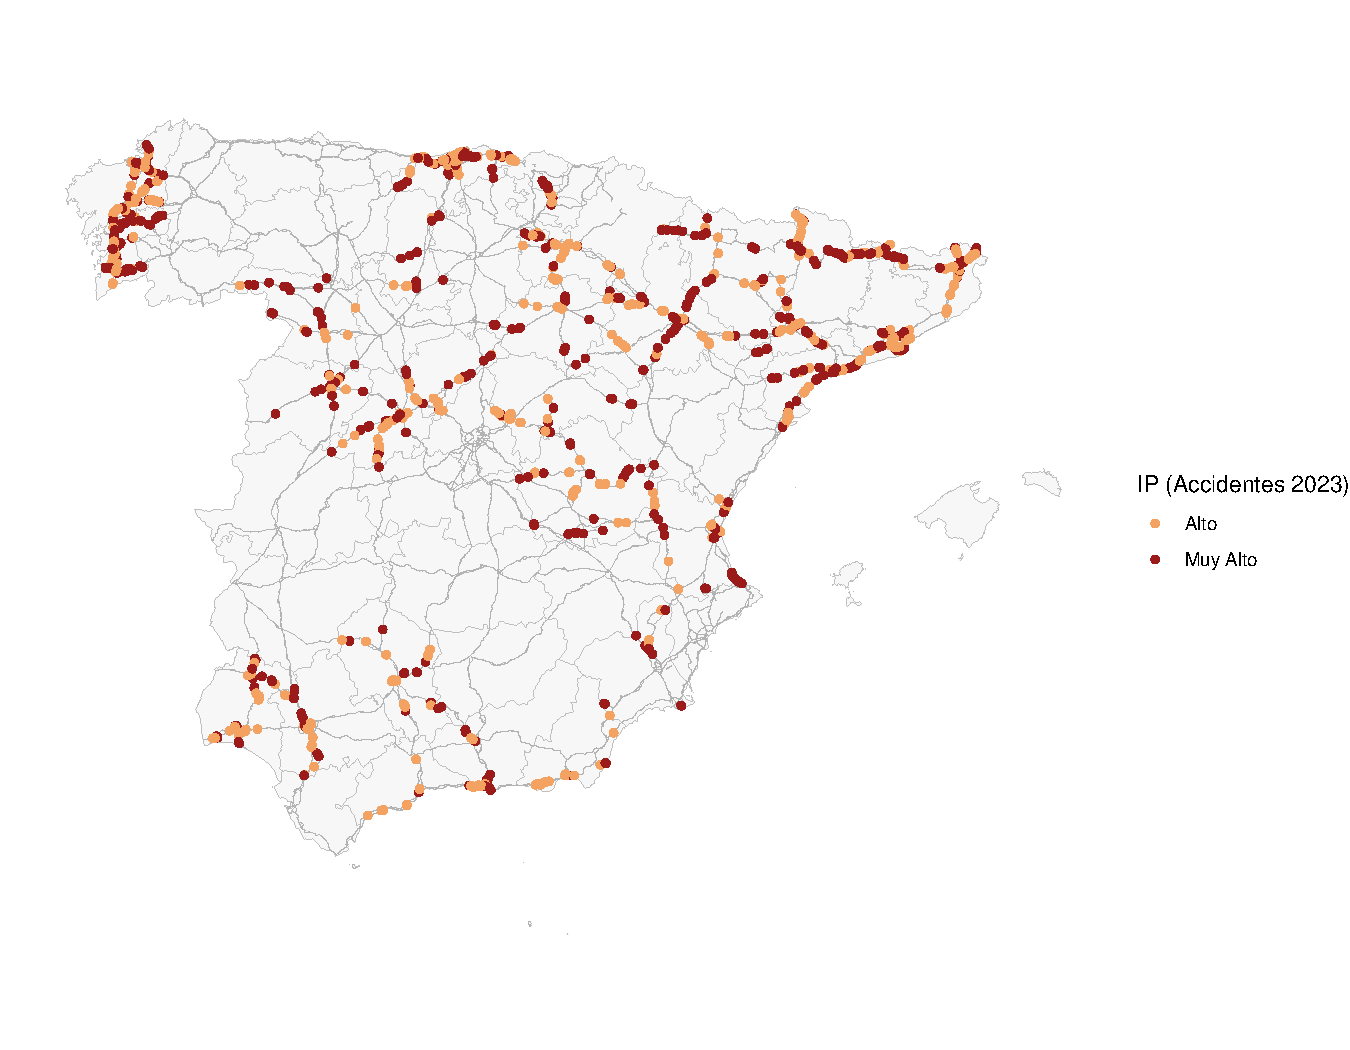
\includegraphics[width=0.85\textwidth]{mapas/mapa_puntos_acc_ip_2023.pdf}
    \caption{Puntos kilométricos de riesgo alto del IP localizados sobre la Red de Carreteras del Estado (Accidentes 2023). Se representan 1918 de los 2949 puntos kilométricos de riesgo alto ($65.0\%$).}
    \label{fig:mapa_puntos_acc_ip_2023}
\end{figure}
 
\begin{figure}[H]
    \centering
    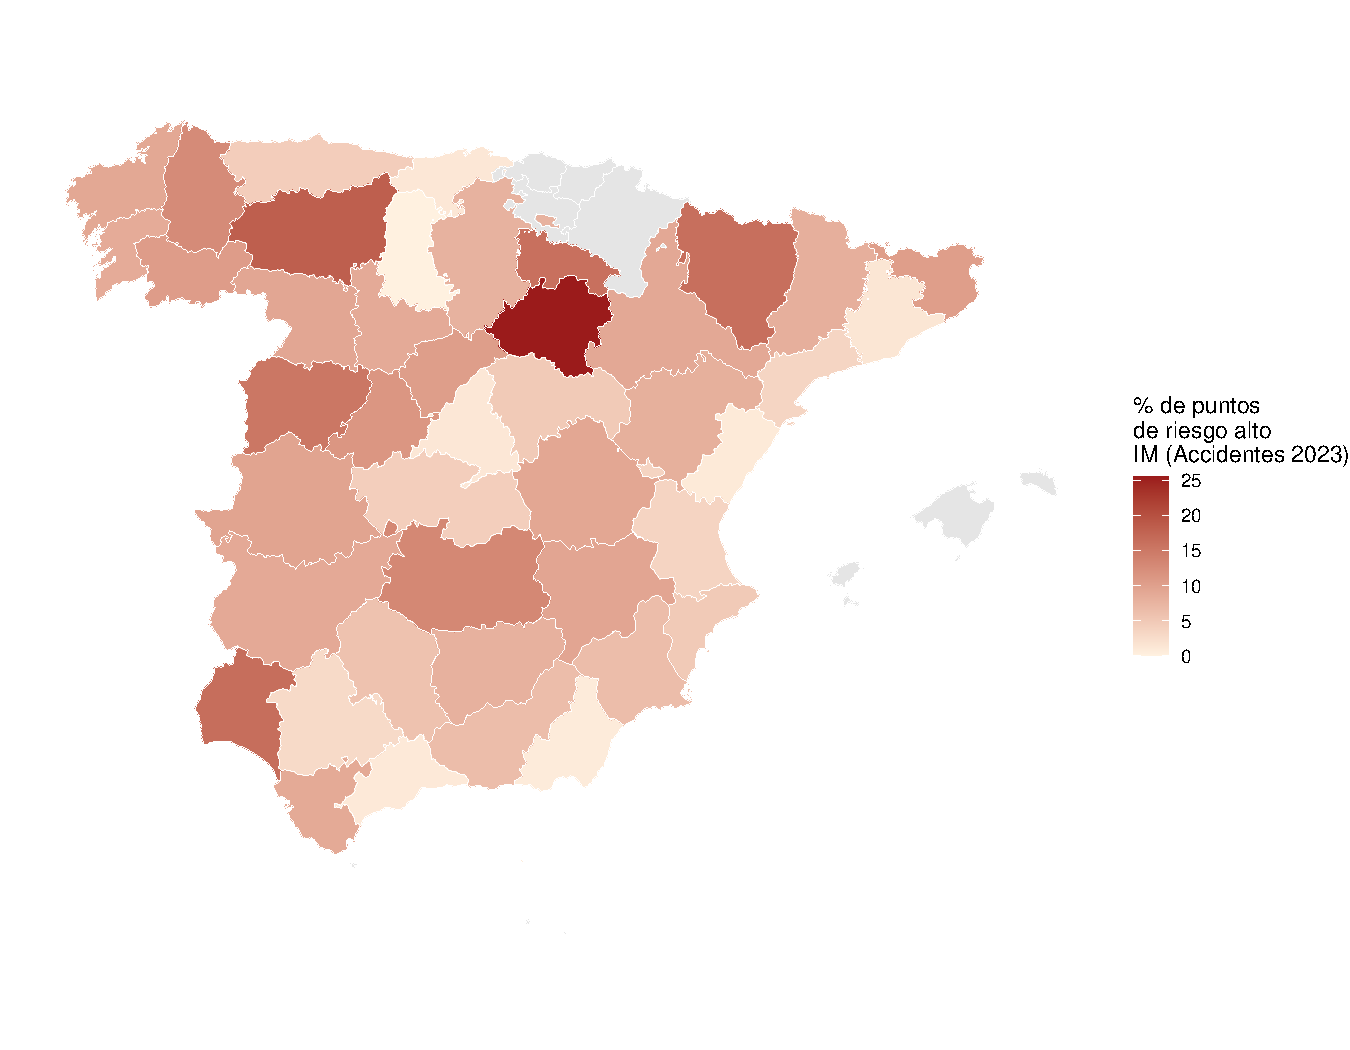
\includegraphics[width=0.85\textwidth]{mapas/mapa_provincias_acc_im_2023.pdf}
    \caption{Porcentaje de puntos kilométricos de riesgo alto del IM en cada provincia (Accidentes 2023).}
    \label{fig:mapa_prov_acc_im_2023}
\end{figure}
 
\begin{figure}[H]
    \centering
    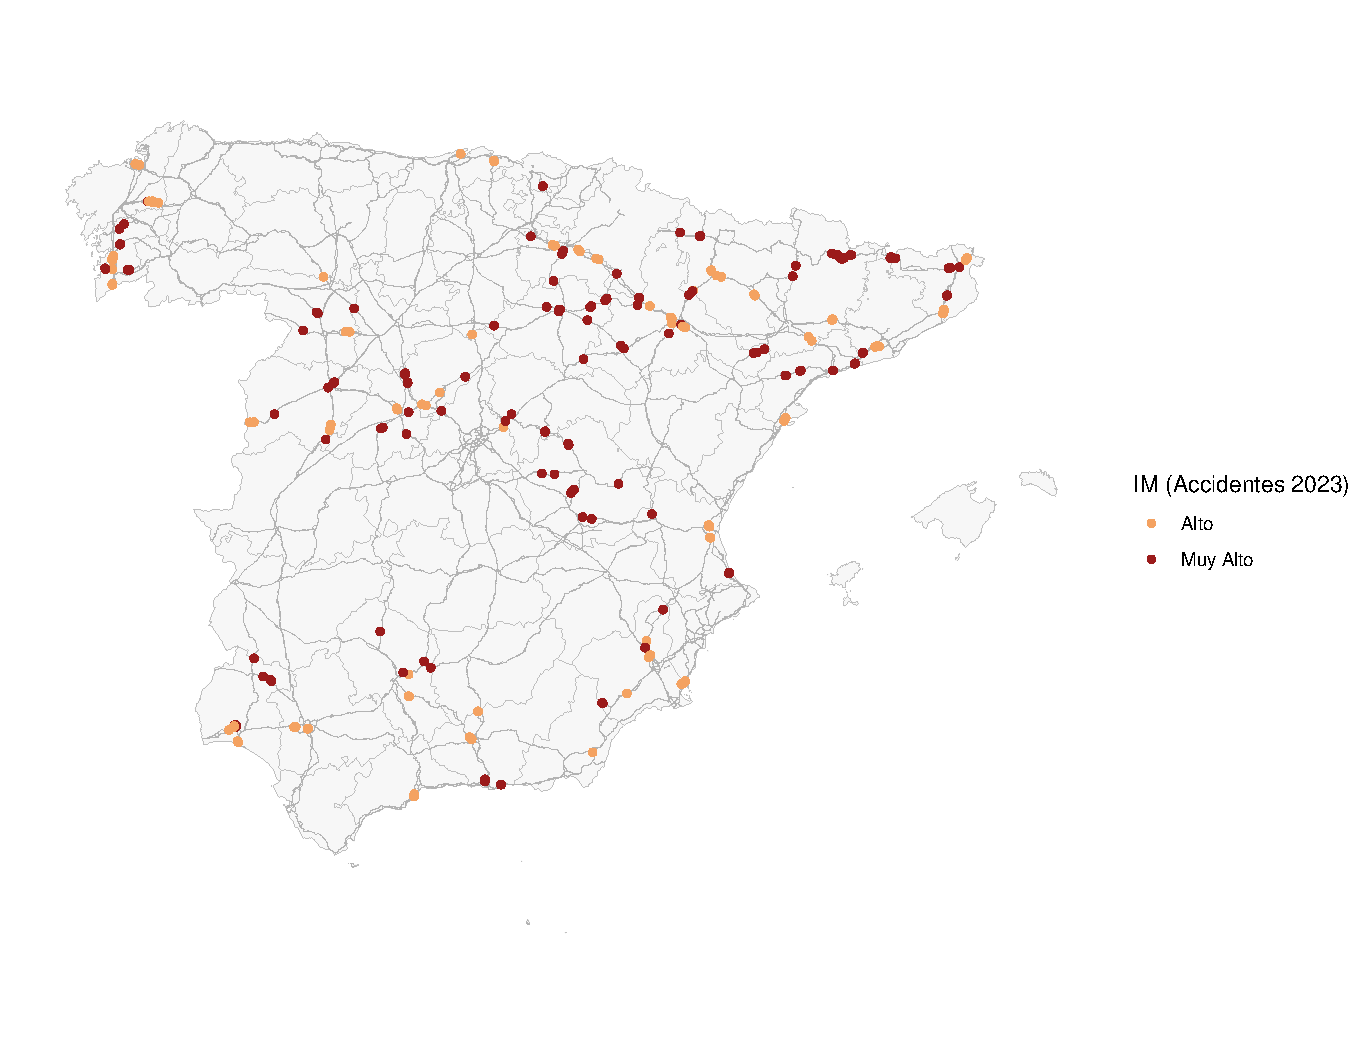
\includegraphics[width=0.85\textwidth]{mapas/mapa_puntos_acc_im_2023.pdf}
    \caption{Puntos kilométricos de riesgo alto del IM localizados sobre la Red de Carreteras del Estado (Accidentes 2023). Se representan 327 de los 505 puntos kilométricos de riesgo alto ($64.8\%$).}
    \label{fig:mapa_puntos_acc_im_2023}
\end{figure}
 
\begin{figure}[H]
    \centering
    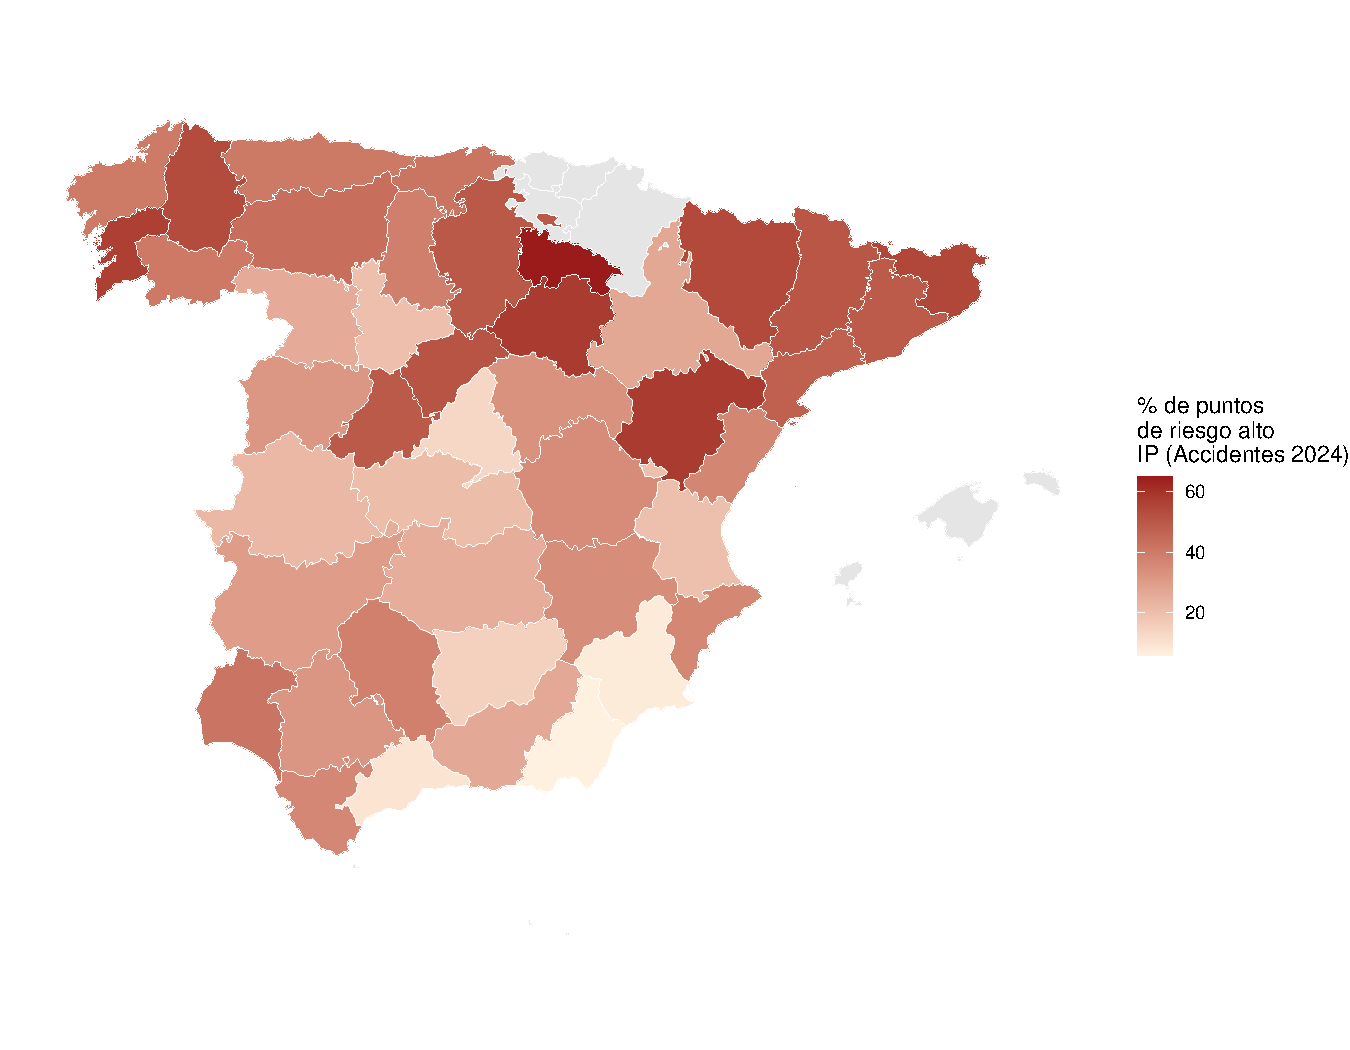
\includegraphics[width=0.85\textwidth]{mapas/mapa_provincias_acc_ip_2024.pdf}
    \caption{Porcentaje de puntos kilométricos de riesgo alto del IP en cada provincia (Accidentes 2024).}
    \label{fig:mapa_prov_acc_ip_2024}
\end{figure}
 
\begin{figure}[H]
    \centering
    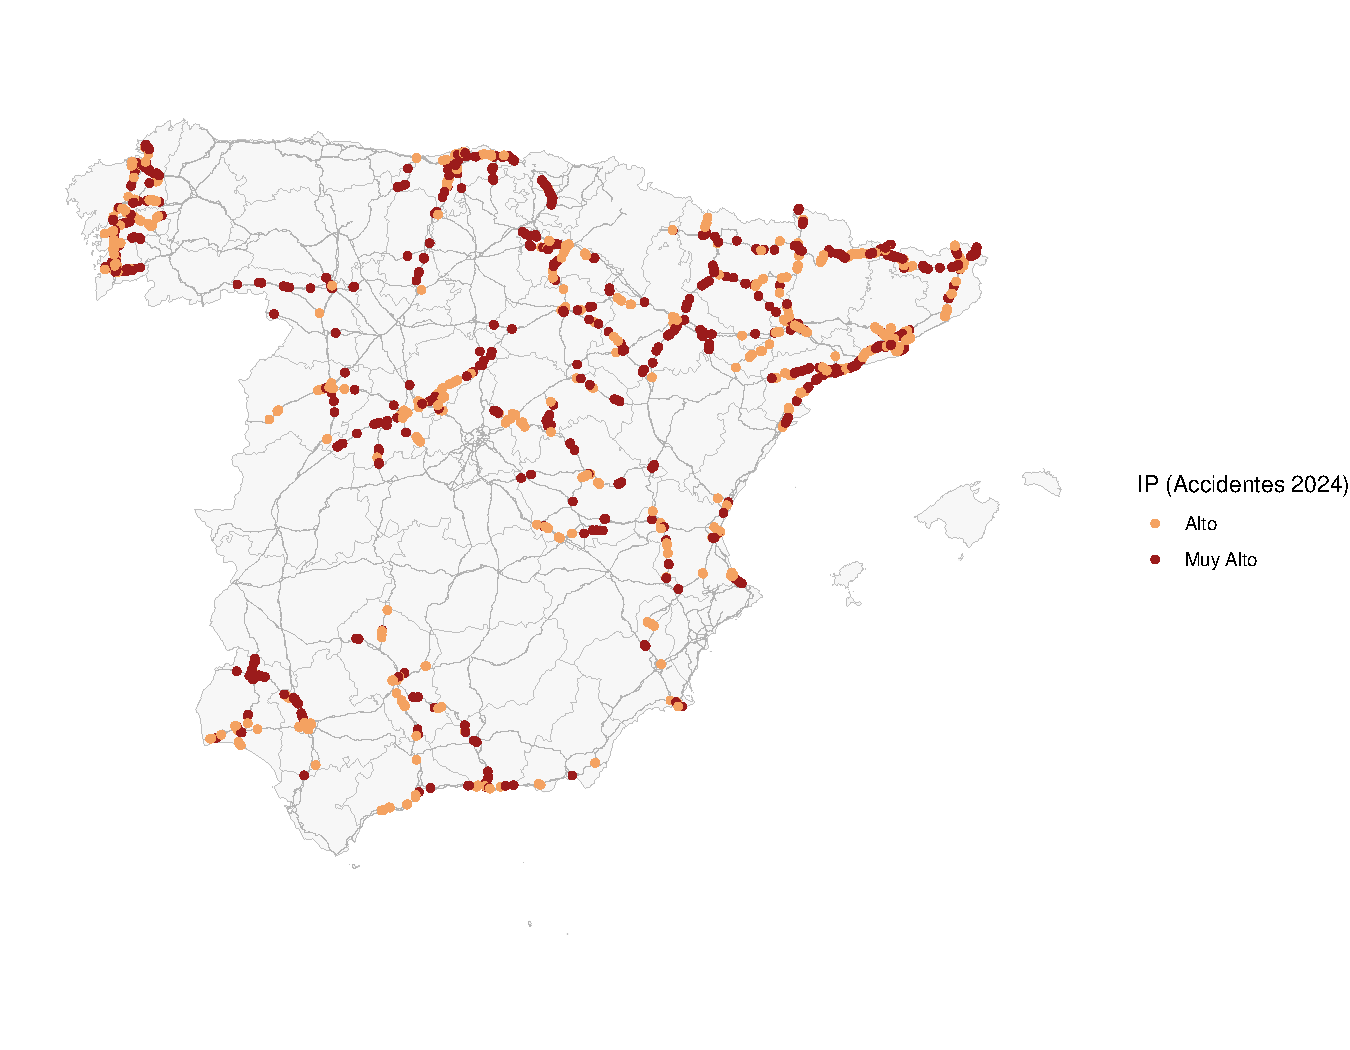
\includegraphics[width=0.85\textwidth]{mapas/mapa_puntos_acc_ip_2024.pdf}
    \caption{Puntos kilométricos de riesgo alto del IP localizados sobre la Red de Carreteras del Estado (Accidentes 2024). Se representan 2062 de los 3068 puntos kilométricos de riesgo alto ($67.2\%$).}
    \label{fig:mapa_puntos_acc_ip_2024}
\end{figure}
 
\begin{figure}[H]
    \centering
    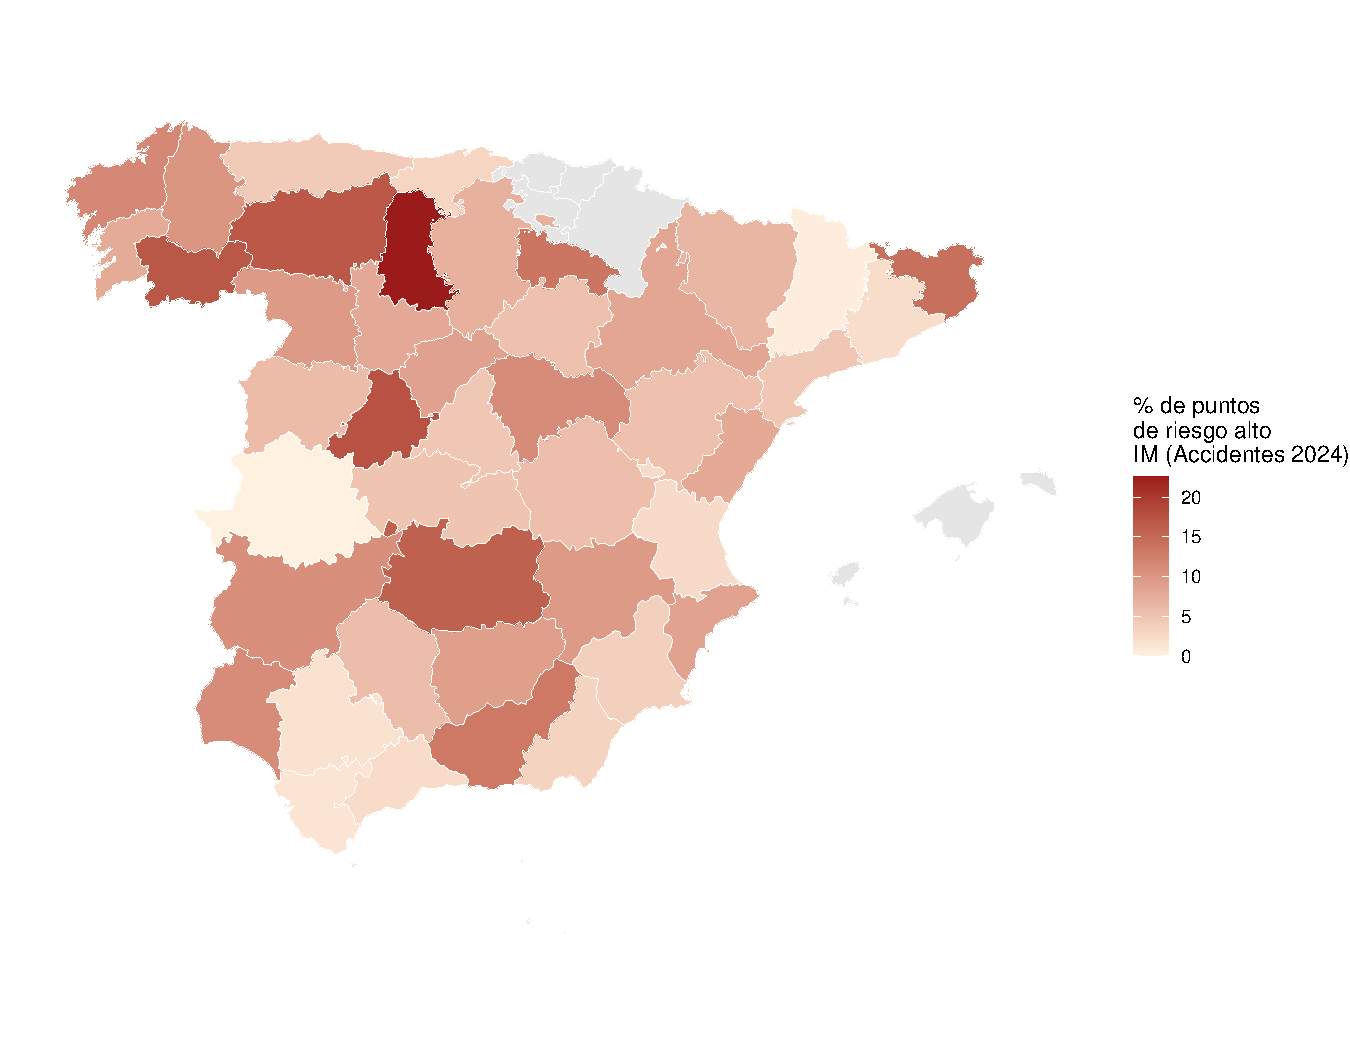
\includegraphics[width=0.85\textwidth]{mapas/mapa_provincias_acc_im_2024.pdf}
    \caption{Porcentaje de puntos kilométricos de riesgo alto del IM en cada provincia (Accidentes 2024).}
    \label{fig:mapa_prov_acc_im_2024}
\end{figure}
 
\begin{figure}[H]
    \centering
    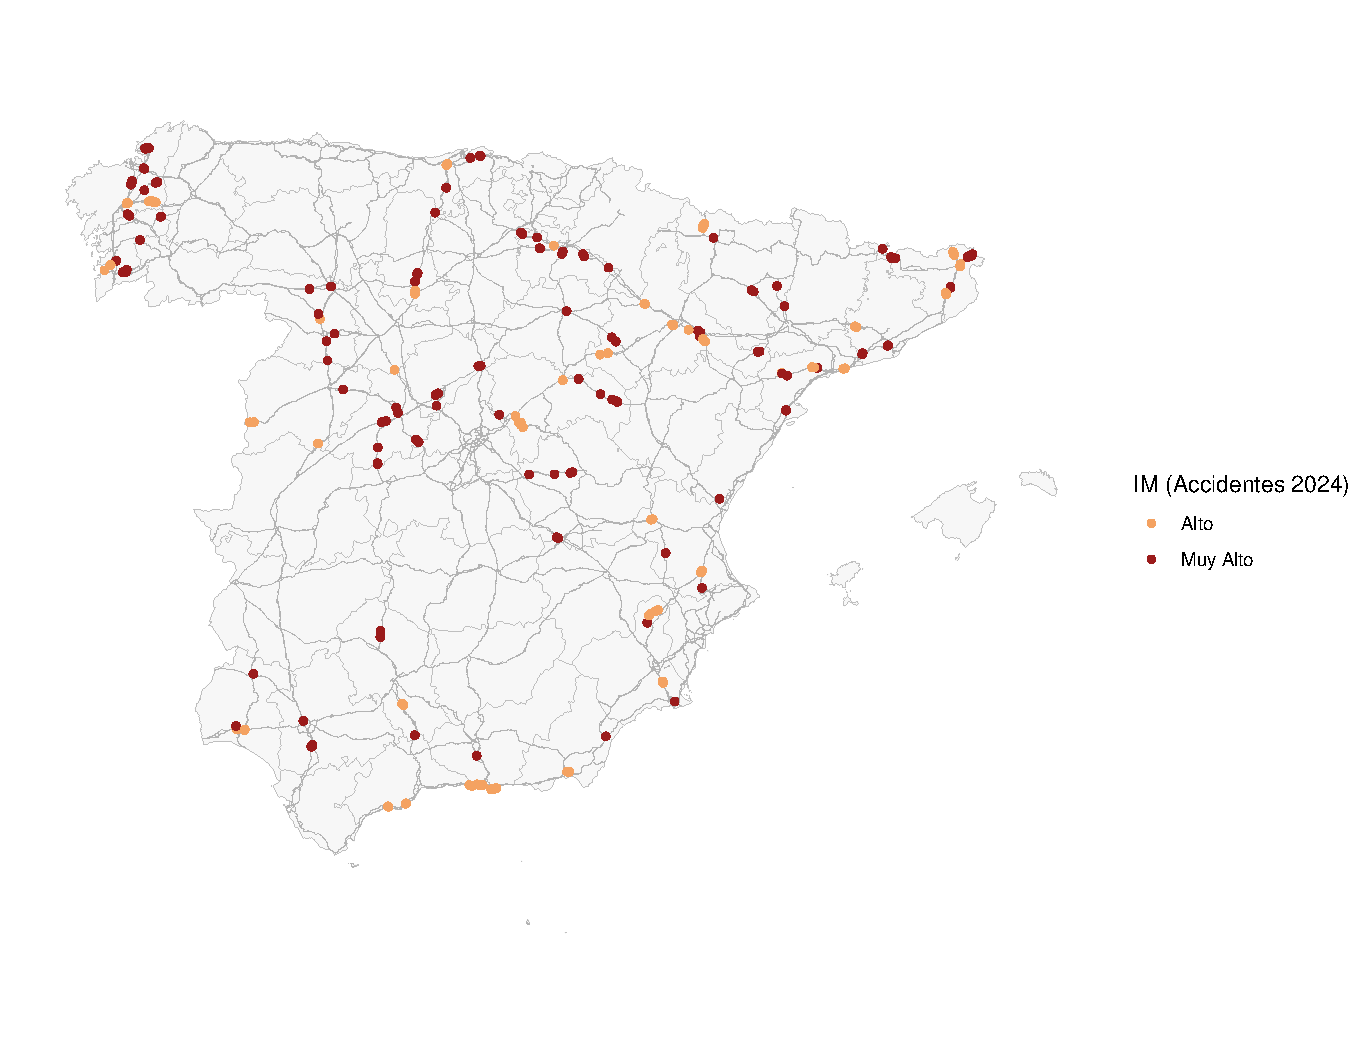
\includegraphics[width=0.85\textwidth]{mapas/mapa_puntos_acc_im_2024.pdf}
    \caption{Puntos kilométricos de riesgo alto del IM localizados sobre la Red de Carreteras del Estado (Accidentes 2024). Se representan 320 de los 563 puntos kilométricos de riesgo alto ($56.8\%$).}
    \label{fig:mapa_puntos_acc_im_2024}
\end{figure}
 




{\footnotesize
\begin{Verbatim}

   codigo R

\end{Verbatim}
}
\end{document}